\documentclass[twoside]{book}

% Packages required by doxygen
\usepackage{fixltx2e}
\usepackage{calc}
\usepackage{doxygen}
\usepackage[export]{adjustbox} % also loads graphicx
\usepackage{graphicx}
\usepackage[utf8]{inputenc}
\usepackage{makeidx}
\usepackage{multicol}
\usepackage{multirow}
\PassOptionsToPackage{warn}{textcomp}
\usepackage{textcomp}
\usepackage[nointegrals]{wasysym}
\usepackage[table]{xcolor}

% Font selection
\usepackage[T1]{fontenc}
\usepackage[scaled=.90]{helvet}
\usepackage{courier}
\usepackage{amssymb}
\usepackage{sectsty}
\renewcommand{\familydefault}{\sfdefault}
\allsectionsfont{%
  \fontseries{bc}\selectfont%
  \color{darkgray}%
}
\renewcommand{\DoxyLabelFont}{%
  \fontseries{bc}\selectfont%
  \color{darkgray}%
}
\newcommand{\+}{\discretionary{\mbox{\scriptsize$\hookleftarrow$}}{}{}}

% Page & text layout
\usepackage{geometry}
\geometry{%
  a4paper,%
  top=2.5cm,%
  bottom=2.5cm,%
  left=2.5cm,%
  right=2.5cm%
}
\tolerance=750
\hfuzz=15pt
\hbadness=750
\setlength{\emergencystretch}{15pt}
\setlength{\parindent}{0cm}
\setlength{\parskip}{0.2cm}
\makeatletter
\renewcommand{\paragraph}{%
  \@startsection{paragraph}{4}{0ex}{-1.0ex}{1.0ex}{%
    \normalfont\normalsize\bfseries\SS@parafont%
  }%
}
\renewcommand{\subparagraph}{%
  \@startsection{subparagraph}{5}{0ex}{-1.0ex}{1.0ex}{%
    \normalfont\normalsize\bfseries\SS@subparafont%
  }%
}
\makeatother

% Headers & footers
\usepackage{fancyhdr}
\pagestyle{fancyplain}
\fancyhead[LE]{\fancyplain{}{\bfseries\thepage}}
\fancyhead[CE]{\fancyplain{}{}}
\fancyhead[RE]{\fancyplain{}{\bfseries\leftmark}}
\fancyhead[LO]{\fancyplain{}{\bfseries\rightmark}}
\fancyhead[CO]{\fancyplain{}{}}
\fancyhead[RO]{\fancyplain{}{\bfseries\thepage}}
\fancyfoot[LE]{\fancyplain{}{}}
\fancyfoot[CE]{\fancyplain{}{}}
\fancyfoot[RE]{\fancyplain{}{\bfseries\scriptsize Generated on Tue Dec 8 2015 17\+:24\+:37 for Labyrinttipeli by Doxygen }}
\fancyfoot[LO]{\fancyplain{}{\bfseries\scriptsize Generated on Tue Dec 8 2015 17\+:24\+:37 for Labyrinttipeli by Doxygen }}
\fancyfoot[CO]{\fancyplain{}{}}
\fancyfoot[RO]{\fancyplain{}{}}
\renewcommand{\footrulewidth}{0.4pt}
\renewcommand{\chaptermark}[1]{%
  \markboth{#1}{}%
}
\renewcommand{\sectionmark}[1]{%
  \markright{\thesection\ #1}%
}

% Indices & bibliography
\usepackage{natbib}
\usepackage[titles]{tocloft}
\setcounter{tocdepth}{3}
\setcounter{secnumdepth}{5}
\makeindex

% Hyperlinks (required, but should be loaded last)
\usepackage{ifpdf}
\ifpdf
  \usepackage[pdftex,pagebackref=true]{hyperref}
\else
  \usepackage[ps2pdf,pagebackref=true]{hyperref}
\fi
\hypersetup{%
  colorlinks=true,%
  linkcolor=blue,%
  citecolor=blue,%
  unicode%
}

% Custom commands
\newcommand{\clearemptydoublepage}{%
  \newpage{\pagestyle{empty}\cleardoublepage}%
}


%===== C O N T E N T S =====

\begin{document}

% Titlepage & ToC
\hypersetup{pageanchor=false,
             bookmarks=true,
             bookmarksnumbered=true,
             pdfencoding=unicode
            }
\pagenumbering{roman}
\begin{titlepage}
\vspace*{7cm}
\begin{center}%
{\Large Labyrinttipeli }\\
\vspace*{1cm}
{\large Generated by Doxygen 1.8.10}\\
\vspace*{0.5cm}
{\small Tue Dec 8 2015 17:24:37}\\
\end{center}
\end{titlepage}
\clearemptydoublepage
\tableofcontents
\clearemptydoublepage
\pagenumbering{arabic}
\hypersetup{pageanchor=true}

%--- Begin generated contents ---
\chapter{Main Page}
\label{index}\hypertarget{index}{}Tämä on O\+H\+J-\/1450 Olio-\/ohjelmoinnin jatkokurssin vuoden 2013 harjoitustyön Labyrinttipeli valmiina annettu sovelluskehys.

Valmiina annetut rajapinnat, tyypit ja luokat löytyvät kaikki nimiavaruudesta {\ttfamily \hyperlink{namespace_julkinen}{Julkinen}}. 
\chapter{Namespace Index}
\section{Namespace List}
Here is a list of all documented namespaces with brief descriptions\+:\begin{DoxyCompactList}
\item\contentsline{section}{\hyperlink{namespace_julkinen}{Julkinen} \\*Luo instanssi pelirajapinnasta }{\pageref{namespace_julkinen}}{}
\end{DoxyCompactList}

\chapter{Hierarchical Index}
\section{Class Hierarchy}
This inheritance list is sorted roughly, but not completely, alphabetically\+:\begin{DoxyCompactList}
\item \contentsline{section}{Alustaja}{\pageref{class_alustaja}}{}
\item \contentsline{section}{Bittikartta}{\pageref{class_bittikartta}}{}
\item \contentsline{section}{Data}{\pageref{class_data}}{}
\item \contentsline{section}{Esine}{\pageref{class_esine}}{}
\item \contentsline{section}{Komentotulkki}{\pageref{class_komentotulkki}}{}
\item \contentsline{section}{Julkinen\+:\+:Koordinaatti}{\pageref{class_julkinen_1_1_koordinaatti}}{}
\item \contentsline{section}{Julkinen\+:\+:Nayttorajapinta}{\pageref{class_julkinen_1_1_nayttorajapinta}}{}
\begin{DoxyCompactList}
\item \contentsline{section}{Naytto}{\pageref{class_naytto}}{}
\end{DoxyCompactList}
\item \contentsline{section}{Naytto\+:\+:P}{\pageref{struct_naytto_1_1_p}}{}
\item \contentsline{section}{Pala}{\pageref{class_pala}}{}
\item \contentsline{section}{Pelaaja}{\pageref{class_pelaaja}}{}
\item \contentsline{section}{Pelin\+Naytto}{\pageref{class_pelin_naytto}}{}
\begin{DoxyCompactList}
\item \contentsline{section}{Pelaaja\+Toiminto}{\pageref{class_pelaaja_toiminto}}{}
\end{DoxyCompactList}
\item \contentsline{section}{Julkinen\+:\+:Pelirajapinta}{\pageref{class_julkinen_1_1_pelirajapinta}}{}
\begin{DoxyCompactList}
\item \contentsline{section}{Peli}{\pageref{class_peli}}{}
\end{DoxyCompactList}
\item \contentsline{section}{Rakentaja}{\pageref{class_rakentaja}}{}
\item \contentsline{section}{Taulukon\+Tuhoaja$<$ T $>$}{\pageref{class_taulukon_tuhoaja}}{}
\item \contentsline{section}{Julkinen\+:\+:Virhe}{\pageref{class_julkinen_1_1_virhe}}{}
\begin{DoxyCompactList}
\item \contentsline{section}{Julkinen\+:\+:Alustusvirhe}{\pageref{class_julkinen_1_1_alustusvirhe}}{}
\item \contentsline{section}{Julkinen\+:\+:Komentovirhe}{\pageref{class_julkinen_1_1_komentovirhe}}{}
\item \contentsline{section}{Julkinen\+:\+:Logiikkavirhe}{\pageref{class_julkinen_1_1_logiikkavirhe}}{}
\item \contentsline{section}{Julkinen\+:\+:Nayttovirhe}{\pageref{class_julkinen_1_1_nayttovirhe}}{}
\item \contentsline{section}{Julkinen\+:\+:Toimintovirhe}{\pageref{class_julkinen_1_1_toimintovirhe}}{}
\item \contentsline{section}{Julkinen\+:\+:Toteuttamaton\+Virhe}{\pageref{class_julkinen_1_1_toteuttamaton_virhe}}{}
\item \contentsline{section}{Julkinen\+:\+:Vaittamavirhe}{\pageref{class_julkinen_1_1_vaittamavirhe}}{}
\begin{DoxyCompactList}
\item \contentsline{section}{Julkinen\+:\+:Esiehtovirhe}{\pageref{class_julkinen_1_1_esiehtovirhe}}{}
\item \contentsline{section}{Julkinen\+:\+:Invarianttivirhe}{\pageref{class_julkinen_1_1_invarianttivirhe}}{}
\item \contentsline{section}{Julkinen\+:\+:Jalkiehtovirhe}{\pageref{class_julkinen_1_1_jalkiehtovirhe}}{}
\end{DoxyCompactList}
\end{DoxyCompactList}
\end{DoxyCompactList}

\chapter{Class Index}
\section{Class List}
Here are the classes, structs, unions and interfaces with brief descriptions\+:\begin{DoxyCompactList}
\item\contentsline{section}{\hyperlink{class_alustaja}{Alustaja} }{\pageref{class_alustaja}}{}
\item\contentsline{section}{\hyperlink{class_julkinen_1_1_alustusvirhe}{Julkinen\+::\+Alustusvirhe} \\*Alustuksessa tapahtuvaa virhettä kuvaava poikkeus }{\pageref{class_julkinen_1_1_alustusvirhe}}{}
\item\contentsline{section}{\hyperlink{class_bittikartta}{Bittikartta} }{\pageref{class_bittikartta}}{}
\item\contentsline{section}{\hyperlink{class_data}{Data} }{\pageref{class_data}}{}
\item\contentsline{section}{\hyperlink{class_julkinen_1_1_esiehtovirhe}{Julkinen\+::\+Esiehtovirhe} \\*Invariantti assertin lähettämän virhe }{\pageref{class_julkinen_1_1_esiehtovirhe}}{}
\item\contentsline{section}{\hyperlink{class_esine}{Esine} \\*Labyrintti-\/pelin esineen tietoluokka }{\pageref{class_esine}}{}
\item\contentsline{section}{\hyperlink{class_julkinen_1_1_invarianttivirhe}{Julkinen\+::\+Invarianttivirhe} \\*Invariantti assertin lähettämän virhe }{\pageref{class_julkinen_1_1_invarianttivirhe}}{}
\item\contentsline{section}{\hyperlink{class_julkinen_1_1_jalkiehtovirhe}{Julkinen\+::\+Jalkiehtovirhe} \\*Jälkiehto assertin lähettämän virhe }{\pageref{class_julkinen_1_1_jalkiehtovirhe}}{}
\item\contentsline{section}{\hyperlink{class_komentotulkki}{Komentotulkki} \\*Komentotulkin toteuttava luokka }{\pageref{class_komentotulkki}}{}
\item\contentsline{section}{\hyperlink{class_julkinen_1_1_komentovirhe}{Julkinen\+::\+Komentovirhe} \\*Käyttäjän antamaa pelikomentoa ei saatu suoritettua }{\pageref{class_julkinen_1_1_komentovirhe}}{}
\item\contentsline{section}{\hyperlink{class_julkinen_1_1_koordinaatti}{Julkinen\+::\+Koordinaatti} \\*Luokka pelin sijainti tietojen esittämiseen }{\pageref{class_julkinen_1_1_koordinaatti}}{}
\item\contentsline{section}{\hyperlink{class_julkinen_1_1_logiikkavirhe}{Julkinen\+::\+Logiikkavirhe} \\*\hyperlink{class_julkinen_1_1_virhe}{Virhe} toimintalogiikka virhetilanteita varten }{\pageref{class_julkinen_1_1_logiikkavirhe}}{}
\item\contentsline{section}{\hyperlink{class_naytto}{Naytto} \\*Labyrintti-\/pelin tulostusluokka }{\pageref{class_naytto}}{}
\item\contentsline{section}{\hyperlink{class_julkinen_1_1_nayttorajapinta}{Julkinen\+::\+Nayttorajapinta} \\*Labyrintti-\/pelin tulostusrajapinta }{\pageref{class_julkinen_1_1_nayttorajapinta}}{}
\item\contentsline{section}{\hyperlink{class_julkinen_1_1_nayttovirhe}{Julkinen\+::\+Nayttovirhe} \\*Näyttörajapinnan tulostusoperaatio ei onnistunut }{\pageref{class_julkinen_1_1_nayttovirhe}}{}
\item\contentsline{section}{\hyperlink{struct_naytto_1_1_p}{Naytto\+::\+P} \\*Tulostuksessa avustava structi }{\pageref{struct_naytto_1_1_p}}{}
\item\contentsline{section}{\hyperlink{class_pala}{Pala} \\*Labyrintti-\/pelin palan tietoluokka }{\pageref{class_pala}}{}
\item\contentsline{section}{\hyperlink{class_pelaaja}{Pelaaja} \\*Labyrintti-\/pelin pelaajan tietoluokka }{\pageref{class_pelaaja}}{}
\item\contentsline{section}{\hyperlink{class_pelaaja_toiminto}{Pelaaja\+Toiminto} \\*Labyrintti-\/pelin pelaajan toimintojen suoritus luokka }{\pageref{class_pelaaja_toiminto}}{}
\item\contentsline{section}{\hyperlink{class_peli}{Peli} \\*Labyrintti-\/pelin pelin toimintojen suorittava luokka }{\pageref{class_peli}}{}
\item\contentsline{section}{\hyperlink{class_pelin_naytto}{Pelin\+Naytto} \\*Labyrintti-\/pelin pelin toimintojen näyttöön piirtäjä }{\pageref{class_pelin_naytto}}{}
\item\contentsline{section}{\hyperlink{class_julkinen_1_1_pelirajapinta}{Julkinen\+::\+Pelirajapinta} \\*Labyrintti-\/pelin ohjausrajapinta }{\pageref{class_julkinen_1_1_pelirajapinta}}{}
\item\contentsline{section}{\hyperlink{class_rakentaja}{Rakentaja} \\*Labyrintti pelin alustaja luokka }{\pageref{class_rakentaja}}{}
\item\contentsline{section}{\hyperlink{class_taulukon_tuhoaja}{Taulukon\+Tuhoaja$<$ T $>$} \\*Tuhoaja-\/funktori taulukoiden säilömiseen std\+::tr1\+::shared\+\_\+ptr\+:n päässä }{\pageref{class_taulukon_tuhoaja}}{}
\item\contentsline{section}{\hyperlink{class_julkinen_1_1_toimintovirhe}{Julkinen\+::\+Toimintovirhe} \\*Toiminnoissa tapahtuvia virheitä kuvaava poikkeus }{\pageref{class_julkinen_1_1_toimintovirhe}}{}
\item\contentsline{section}{\hyperlink{class_julkinen_1_1_toteuttamaton_virhe}{Julkinen\+::\+Toteuttamaton\+Virhe} \\*Toimintoa ei ole vielä toteutettu }{\pageref{class_julkinen_1_1_toteuttamaton_virhe}}{}
\item\contentsline{section}{\hyperlink{class_julkinen_1_1_vaittamavirhe}{Julkinen\+::\+Vaittamavirhe} \\*Assertio rajapinnan käyttämä virhetyyppi }{\pageref{class_julkinen_1_1_vaittamavirhe}}{}
\item\contentsline{section}{\hyperlink{class_julkinen_1_1_virhe}{Julkinen\+::\+Virhe} \\*Labyrintin poikkeusten kantaluokka }{\pageref{class_julkinen_1_1_virhe}}{}
\end{DoxyCompactList}

\chapter{File Index}
\section{File List}
Here is a list of all documented files with brief descriptions\+:\begin{DoxyCompactList}
\item\contentsline{section}{\hyperlink{alustusvirhe_8hh}{alustusvirhe.\+hh} \\*Alustusvirhe-\/luokan esittely. ( }{\pageref{alustusvirhe_8hh}}{}
\item\contentsline{section}{\hyperlink{_data_8hpp}{Data.\+hpp} \\*Data-\/luokan esittely }{\pageref{_data_8hpp}}{}
\item\contentsline{section}{\hyperlink{debug_8hh}{debug.\+hh} \\*Debuggauksen apumakro }{\pageref{debug_8hh}}{}
\item\contentsline{section}{\hyperlink{_esine_8hpp}{Esine.\+hpp} \\*Esine-\/luokan esittely }{\pageref{_esine_8hpp}}{}
\item\contentsline{section}{\hyperlink{komentovirhe_8hh}{komentovirhe.\+hh} \\*Komentovirhe-\/luokan esittely }{\pageref{komentovirhe_8hh}}{}
\item\contentsline{section}{\hyperlink{koordinaatti_8hh}{koordinaatti.\+hh} \\*Koordinaatti-\/luokan esittely. ( }{\pageref{koordinaatti_8hh}}{}
\item\contentsline{section}{\hyperlink{logiikkavirhe_8hh}{logiikkavirhe.\+hh} \\*Logiikkavirhe-\/luokan esittely }{\pageref{logiikkavirhe_8hh}}{}
\item\contentsline{section}{\hyperlink{luettelotyypit_8hh}{luettelotyypit.\+hh} \\*Pelirajapinta-\/luokan esittely. ( }{\pageref{luettelotyypit_8hh}}{}
\item\contentsline{section}{\hyperlink{nayttorajapinta_8hh}{nayttorajapinta.\+hh} \\*Rajapinta pelin luomiseksi ( }{\pageref{nayttorajapinta_8hh}}{}
\item\contentsline{section}{\hyperlink{nayttovirhe_8hh}{nayttovirhe.\+hh} \\*Nayttovirhe-\/luokan esittely }{\pageref{nayttovirhe_8hh}}{}
\item\contentsline{section}{\hyperlink{_pala_8hpp}{Pala.\+hpp} \\*Pala-\/luokan esittely }{\pageref{_pala_8hpp}}{}
\item\contentsline{section}{\hyperlink{_pelaaja_8hpp}{Pelaaja.\+hpp} \\*Pelaaja-\/luokan esittely }{\pageref{_pelaaja_8hpp}}{}
\item\contentsline{section}{\hyperlink{_pelaaja_toiminto_8hpp}{Pelaaja\+Toiminto.\+hpp} \\*Pelaaja\+Toiminto-\/luokan esittely }{\pageref{_pelaaja_toiminto_8hpp}}{}
\item\contentsline{section}{\hyperlink{_peli_8hpp}{Peli.\+hpp} \\*Peli-\/luokan esittely }{\pageref{_peli_8hpp}}{}
\item\contentsline{section}{\hyperlink{_pelin_naytto_8hpp}{Pelin\+Naytto.\+hpp} \\*Pelin\+Naytto-\/luokan esittely }{\pageref{_pelin_naytto_8hpp}}{}
\item\contentsline{section}{\hyperlink{pelirajapinta_8hh}{pelirajapinta.\+hh} \\*Pelirajapinta-\/luokan esittely. ( }{\pageref{pelirajapinta_8hh}}{}
\item\contentsline{section}{\hyperlink{pelitehdas_8hh}{pelitehdas.\+hh} \\*Rajapinta pelin luomiseksi }{\pageref{pelitehdas_8hh}}{}
\item\contentsline{section}{\hyperlink{toimintovirhe_8hh}{toimintovirhe.\+hh} \\*Toimintovirhe-\/luokan esittely }{\pageref{toimintovirhe_8hh}}{}
\item\contentsline{section}{\hyperlink{toteuttamaton__virhe_8hh}{toteuttamaton\+\_\+virhe.\+hh} \\*Toteuttamaton\+Virhe-\/luokan esittely }{\pageref{toteuttamaton__virhe_8hh}}{}
\item\contentsline{section}{\hyperlink{vaittama_8hh}{vaittama.\+hh} \\*Väittämien tarkistustyökalujen esittelyt }{\pageref{vaittama_8hh}}{}
\item\contentsline{section}{\hyperlink{virhe_8hh}{virhe.\+hh} \\*Virhe-\/luokan esittely }{\pageref{virhe_8hh}}{}
\item\contentsline{section}{valmiiden\+\_\+toteutus/\hyperlink{_alustaja_8cc}{Alustaja.\+cc} \\*Alustaja-\/luokan toteutus( }{\pageref{_alustaja_8cc}}{}
\item\contentsline{section}{valmiiden\+\_\+toteutus/\hyperlink{alustusvirhe_8cc}{alustusvirhe.\+cc} \\*Alustusvirhe-\/luokan toteutus. ( }{\pageref{alustusvirhe_8cc}}{}
\item\contentsline{section}{valmiiden\+\_\+toteutus/\hyperlink{_bittikartta_8cc}{Bittikartta.\+cc} \\*Bittikartta-\/luokan toteutus ( }{\pageref{_bittikartta_8cc}}{}
\item\contentsline{section}{valmiiden\+\_\+toteutus/\hyperlink{esiehtovirhe_8cc}{esiehtovirhe.\+cc} \\*\hyperlink{class_julkinen_1_1_esiehtovirhe}{Julkinen\+::\+Esiehtovirhe}-\/luokan toteutus }{\pageref{esiehtovirhe_8cc}}{}
\item\contentsline{section}{valmiiden\+\_\+toteutus/\hyperlink{hyodykkeet_8cc}{hyodykkeet.\+cc} \\*Apufunktioiden toteutukset }{\pageref{hyodykkeet_8cc}}{}
\item\contentsline{section}{valmiiden\+\_\+toteutus/\hyperlink{hyodykkeet_8hh}{hyodykkeet.\+hh} \\*Apufunktioiden esittelyjä }{\pageref{hyodykkeet_8hh}}{}
\item\contentsline{section}{valmiiden\+\_\+toteutus/\hyperlink{invarianttivirhe_8cc}{invarianttivirhe.\+cc} \\*\hyperlink{class_julkinen_1_1_invarianttivirhe}{Julkinen\+::\+Invarianttivirhe}-\/luokan toteutus }{\pageref{invarianttivirhe_8cc}}{}
\item\contentsline{section}{valmiiden\+\_\+toteutus/\hyperlink{jalkiehtovirhe_8cc}{jalkiehtovirhe.\+cc} \\*\hyperlink{class_julkinen_1_1_jalkiehtovirhe}{Julkinen\+::\+Jalkiehtovirhe}-\/luokan toteutus }{\pageref{jalkiehtovirhe_8cc}}{}
\item\contentsline{section}{valmiiden\+\_\+toteutus/\hyperlink{komentotulkki_8cc}{komentotulkki.\+cc} \\*Komentotulkki-\/luokan toteutus. ( }{\pageref{komentotulkki_8cc}}{}
\item\contentsline{section}{valmiiden\+\_\+toteutus/\hyperlink{komentovirhe_8cc}{komentovirhe.\+cc} \\*\hyperlink{class_julkinen_1_1_komentovirhe}{Julkinen\+::\+Komentovirhe}-\/luokan toteutus. ( }{\pageref{komentovirhe_8cc}}{}
\item\contentsline{section}{valmiiden\+\_\+toteutus/\hyperlink{koordinaatti_8cc}{koordinaatti.\+cc} \\*Koordinaatti-\/luokan toteutus. ( }{\pageref{koordinaatti_8cc}}{}
\item\contentsline{section}{valmiiden\+\_\+toteutus/\hyperlink{labyrintti_8cc}{labyrintti.\+cc} \\*Labyrintti pelin pääohjelma ( }{\pageref{labyrintti_8cc}}{}
\item\contentsline{section}{valmiiden\+\_\+toteutus/\hyperlink{logiikkavirhe_8cc}{logiikkavirhe.\+cc} \\*Logiikkavirhe-\/luokan toteutus. ( }{\pageref{logiikkavirhe_8cc}}{}
\item\contentsline{section}{valmiiden\+\_\+toteutus/\hyperlink{naytto_8cc}{naytto.\+cc} \\*Naytto-\/luokkan toteutus ( }{\pageref{naytto_8cc}}{}
\item\contentsline{section}{valmiiden\+\_\+toteutus/\hyperlink{nayttovirhe_8cc}{nayttovirhe.\+cc} \\*Nayttovirhe-\/luokan toteutus. ( }{\pageref{nayttovirhe_8cc}}{}
\item\contentsline{section}{valmiiden\+\_\+toteutus/\hyperlink{rakentaja_8cc}{rakentaja.\+cc} \\*Rakentaa-\/luokan toteutus. ( }{\pageref{rakentaja_8cc}}{}
\item\contentsline{section}{valmiiden\+\_\+toteutus/\hyperlink{toimintovirhe_8cc}{toimintovirhe.\+cc} \\*Toimintovirhe-\/luokan toteutus. ( }{\pageref{toimintovirhe_8cc}}{}
\item\contentsline{section}{valmiiden\+\_\+toteutus/\hyperlink{toteuttamaton__virhe_8cc}{toteuttamaton\+\_\+virhe.\+cc} \\*\hyperlink{class_julkinen_1_1_toteuttamaton_virhe}{Julkinen\+::\+Toteuttamaton\+Virhe}-\/luokan toteutus. ( }{\pageref{toteuttamaton__virhe_8cc}}{}
\item\contentsline{section}{valmiiden\+\_\+toteutus/\hyperlink{vaittama_8cc}{vaittama.\+cc} \\*Pysyv�isv�itt�mien tarkistamisen toteutus }{\pageref{vaittama_8cc}}{}
\item\contentsline{section}{valmiiden\+\_\+toteutus/\hyperlink{vaittamavirhe_8cc}{vaittamavirhe.\+cc} \\*\hyperlink{class_julkinen_1_1_vaittamavirhe}{Julkinen\+::\+Vaittamavirhe}-\/luokan toteutus }{\pageref{vaittamavirhe_8cc}}{}
\item\contentsline{section}{valmiiden\+\_\+toteutus/\hyperlink{virhe_8cc}{virhe.\+cc} \\*\hyperlink{class_julkinen_1_1_virhe}{Julkinen\+::\+Virhe}-\/luokan toteutus. ( }{\pageref{virhe_8cc}}{}
\item\contentsline{section}{valmiiden\+\_\+toteutus/include/\hyperlink{_alustaja_8hh}{Alustaja.\+hh} \\*Labyrintti-\/pelin alustuksen apuluokka ( }{\pageref{_alustaja_8hh}}{}
\item\contentsline{section}{valmiiden\+\_\+toteutus/include/\hyperlink{_bittikartta_8hh}{Bittikartta.\+hh} \\*Labyrintti-\/pelin tulostuksen apuluokka ( }{\pageref{_bittikartta_8hh}}{}
\item\contentsline{section}{valmiiden\+\_\+toteutus/include/\hyperlink{esiehtovirhe_8hh}{esiehtovirhe.\+hh} \\*\hyperlink{class_julkinen_1_1_esiehtovirhe}{Julkinen\+::\+Esiehtovirhe}-\/luokan esittely }{\pageref{esiehtovirhe_8hh}}{}
\item\contentsline{section}{valmiiden\+\_\+toteutus/include/\hyperlink{include_8hh}{include.\+hh} \\*P��ohjelman kirjastojen liitt�mistiedosto }{\pageref{include_8hh}}{}
\item\contentsline{section}{valmiiden\+\_\+toteutus/include/\hyperlink{invarianttivirhe_8hh}{invarianttivirhe.\+hh} \\*\hyperlink{class_julkinen_1_1_invarianttivirhe}{Julkinen\+::\+Invarianttivirhe}-\/luokan esittely }{\pageref{invarianttivirhe_8hh}}{}
\item\contentsline{section}{valmiiden\+\_\+toteutus/include/\hyperlink{jalkiehtovirhe_8hh}{jalkiehtovirhe.\+hh} \\*\hyperlink{class_julkinen_1_1_jalkiehtovirhe}{Julkinen\+::\+Jalkiehtovirhe}-\/luokan esittely }{\pageref{jalkiehtovirhe_8hh}}{}
\item\contentsline{section}{valmiiden\+\_\+toteutus/include/\hyperlink{komentotulkki_8hh}{komentotulkki.\+hh} \\*Komentotulkki-\/luokan esittely. ( }{\pageref{komentotulkki_8hh}}{}
\item\contentsline{section}{valmiiden\+\_\+toteutus/include/\hyperlink{naytto_8hh}{naytto.\+hh} \\*Naytto-\/luokan esittely. ( }{\pageref{naytto_8hh}}{}
\item\contentsline{section}{valmiiden\+\_\+toteutus/include/\hyperlink{rakentaja_8hh}{rakentaja.\+hh} \\*Rakentaja-\/luokan esittely. ( }{\pageref{rakentaja_8hh}}{}
\item\contentsline{section}{valmiiden\+\_\+toteutus/include/\hyperlink{vaittamavirhe_8hh}{vaittamavirhe.\+hh} \\*\hyperlink{class_julkinen_1_1_vaittamavirhe}{Julkinen\+::\+Vaittamavirhe}-\/luokan esittely }{\pageref{vaittamavirhe_8hh}}{}
\end{DoxyCompactList}

\chapter{Namespace Documentation}
\hypertarget{namespace_julkinen}{}\section{Julkinen Namespace Reference}
\label{namespace_julkinen}\index{Julkinen@{Julkinen}}


Luo instanssi pelirajapinnasta.  


\subsection*{Classes}
\begin{DoxyCompactItemize}
\item 
class \hyperlink{class_julkinen_1_1_alustusvirhe}{Alustusvirhe}
\begin{DoxyCompactList}\small\item\em Alustuksessa tapahtuvaa virhettä kuvaava poikkeus. \end{DoxyCompactList}\item 
class \hyperlink{class_julkinen_1_1_esiehtovirhe}{Esiehtovirhe}
\begin{DoxyCompactList}\small\item\em Invariantti assertin lähettämän virhe. \end{DoxyCompactList}\item 
class \hyperlink{class_julkinen_1_1_invarianttivirhe}{Invarianttivirhe}
\begin{DoxyCompactList}\small\item\em Invariantti assertin lähettämän virhe. \end{DoxyCompactList}\item 
class \hyperlink{class_julkinen_1_1_jalkiehtovirhe}{Jalkiehtovirhe}
\begin{DoxyCompactList}\small\item\em Jälkiehto assertin lähettämän virhe. \end{DoxyCompactList}\item 
class \hyperlink{class_julkinen_1_1_komentovirhe}{Komentovirhe}
\begin{DoxyCompactList}\small\item\em Käyttäjän antamaa pelikomentoa ei saatu suoritettua. \end{DoxyCompactList}\item 
class \hyperlink{class_julkinen_1_1_koordinaatti}{Koordinaatti}
\begin{DoxyCompactList}\small\item\em Luokka pelin sijainti tietojen esittämiseen. \end{DoxyCompactList}\item 
class \hyperlink{class_julkinen_1_1_logiikkavirhe}{Logiikkavirhe}
\begin{DoxyCompactList}\small\item\em \hyperlink{class_julkinen_1_1_virhe}{Virhe} toimintalogiikka virhetilanteita varten. \end{DoxyCompactList}\item 
class \hyperlink{class_julkinen_1_1_nayttorajapinta}{Nayttorajapinta}
\begin{DoxyCompactList}\small\item\em Labyrintti-\/pelin tulostusrajapinta. \end{DoxyCompactList}\item 
class \hyperlink{class_julkinen_1_1_nayttovirhe}{Nayttovirhe}
\begin{DoxyCompactList}\small\item\em Näyttörajapinnan tulostusoperaatio ei onnistunut. \end{DoxyCompactList}\item 
class \hyperlink{class_julkinen_1_1_pelirajapinta}{Pelirajapinta}
\begin{DoxyCompactList}\small\item\em Labyrintti-\/pelin ohjausrajapinta. \end{DoxyCompactList}\item 
class \hyperlink{class_julkinen_1_1_toimintovirhe}{Toimintovirhe}
\begin{DoxyCompactList}\small\item\em Toiminnoissa tapahtuvia virheitä kuvaava poikkeus. \end{DoxyCompactList}\item 
class \hyperlink{class_julkinen_1_1_toteuttamaton_virhe}{Toteuttamaton\+Virhe}
\begin{DoxyCompactList}\small\item\em Toimintoa ei ole vielä toteutettu. \end{DoxyCompactList}\item 
class \hyperlink{class_julkinen_1_1_vaittamavirhe}{Vaittamavirhe}
\begin{DoxyCompactList}\small\item\em Assertio rajapinnan käyttämä virhetyyppi. \end{DoxyCompactList}\item 
class \hyperlink{class_julkinen_1_1_virhe}{Virhe}
\begin{DoxyCompactList}\small\item\em Labyrintin poikkeusten kantaluokka. \end{DoxyCompactList}\end{DoxyCompactItemize}
\subsection*{Enumerations}
\begin{DoxyCompactItemize}
\item 
enum \hyperlink{namespace_julkinen_a81b50e3c6f21c0c1c46e186592107c3c}{Suunta} \{ \\*
\hyperlink{namespace_julkinen_a81b50e3c6f21c0c1c46e186592107c3cacae80e18deb2f6685d0bf0f174042ec2}{A\+L\+A\+S}, 
\hyperlink{namespace_julkinen_a81b50e3c6f21c0c1c46e186592107c3ca989d727d65ca4aea941b51638e642596}{A\+U\+T\+O\+M\+A\+A\+T\+T\+I}, 
\hyperlink{namespace_julkinen_a81b50e3c6f21c0c1c46e186592107c3cafd8f13dddbcf5e33a9c33a4cdae76f59}{O\+I\+K\+E\+A\+L\+L\+E}, 
\hyperlink{namespace_julkinen_a81b50e3c6f21c0c1c46e186592107c3ca4b3b91fdb43fdb60e03fb47b23c78e03}{V\+A\+S\+E\+M\+M\+A\+L\+L\+E}, 
\\*
\hyperlink{namespace_julkinen_a81b50e3c6f21c0c1c46e186592107c3caa9a06721d0cc8ff51b1071d3962841ee}{Y\+L\+O\+S}, 
\hyperlink{namespace_julkinen_a81b50e3c6f21c0c1c46e186592107c3cafa60a1b03bc49af14fb90b7026f94957}{P\+A\+I\+K\+A\+L\+L\+A\+A\+N}
 \}\begin{DoxyCompactList}\small\item\em Pelaajan liikumissuunnat. \end{DoxyCompactList}
\item 
enum \hyperlink{namespace_julkinen_afc26052e09d0b2214f749492cc5fff19}{Erikoispala\+Tyyppi} \{ \hyperlink{namespace_julkinen_afc26052e09d0b2214f749492cc5fff19a67d9c76baa2a4eec4ca132c15bd567b5}{N\+O\+R\+M\+A\+A\+L\+I}, 
\hyperlink{namespace_julkinen_afc26052e09d0b2214f749492cc5fff19aec227daa1859a2163571035e354c97b4}{T\+E\+L\+E\+P\+O\+R\+T\+T\+I}, 
\hyperlink{namespace_julkinen_afc26052e09d0b2214f749492cc5fff19aa50081048583c91c88ed285cad5d3080}{S\+I\+U\+N\+A\+T\+T\+U}, 
\hyperlink{namespace_julkinen_afc26052e09d0b2214f749492cc5fff19a8a097f13eb73d7bf4d8cd14dea73ce24}{K\+I\+R\+O\+T\+T\+U}
 \}\begin{DoxyCompactList}\small\item\em Esineiden tyyppitieto. \end{DoxyCompactList}
\item 
enum \hyperlink{namespace_julkinen_ad9a0a9e01af78249f584a93b03db4329}{Pelaaja\+Tyyppi} \{ \hyperlink{namespace_julkinen_ad9a0a9e01af78249f584a93b03db4329ac071c9196447e9db07e03619140a21a9}{I\+H\+M\+I\+N\+E\+N}, 
\hyperlink{namespace_julkinen_ad9a0a9e01af78249f584a93b03db4329a72363d3abdcf0ff5a5318785a7d18363}{T\+I\+E\+T\+O\+K\+O\+N\+E}
 \}\begin{DoxyCompactList}\small\item\em Tieto millainen pelaaja on kyseessä \end{DoxyCompactList}
\item 
enum \hyperlink{namespace_julkinen_a272c70e0503191a485c8a9cd4281e6f5}{Pala\+Tyyppi} \{ \hyperlink{namespace_julkinen_a272c70e0503191a485c8a9cd4281e6f5abda0f6d812200f15d8486fa03a5e24d5}{I\+P\+A\+L\+A}, 
\hyperlink{namespace_julkinen_a272c70e0503191a485c8a9cd4281e6f5aca28caf9f024aa0f392fe0242f5e31f4}{L\+P\+A\+L\+A}, 
\hyperlink{namespace_julkinen_a272c70e0503191a485c8a9cd4281e6f5ad52333f7493bd772341097ab62f7eba3}{T\+P\+A\+L\+A}
 \}\begin{DoxyCompactList}\small\item\em Tieto siitä minkämuotoinen pala on kyseessä \end{DoxyCompactList}
\item 
enum \hyperlink{namespace_julkinen_acce0eefc4c90f907dd5fb319b0d05872}{Reuna} \{ \\*
\hyperlink{namespace_julkinen_acce0eefc4c90f907dd5fb319b0d05872ae751031a265231a493641ba564930530}{A\+L\+A}, 
\hyperlink{namespace_julkinen_acce0eefc4c90f907dd5fb319b0d05872ae4725f066287e0db7262b3981a2756d6}{O\+I\+K\+E\+A}, 
\hyperlink{namespace_julkinen_acce0eefc4c90f907dd5fb319b0d05872a15b788f98845dd777cba865f4ad12cce}{V\+A\+S\+E\+N}, 
\hyperlink{namespace_julkinen_acce0eefc4c90f907dd5fb319b0d05872ad0f36cc10711b6b9d5141e86d02e8040}{Y\+L\+A}, 
\\*
\hyperlink{namespace_julkinen_acce0eefc4c90f907dd5fb319b0d05872a0ce6aecd0ad5ab9e7311506949a7d2c8}{E\+I\+O\+L\+E}
 \}\begin{DoxyCompactList}\small\item\em Tieto mille reunalle irtopala työnnettiin. \end{DoxyCompactList}
\item 
\hypertarget{namespace_julkinen_a2a2bfc4f2a56fb3f3fa143103534a14f}{}enum \hyperlink{namespace_julkinen_a2a2bfc4f2a56fb3f3fa143103534a14f}{Vaittama\+Tyyppi} \{ {\bfseries I\+N\+V\+A\+R\+I\+A\+N\+T\+T\+I\+V\+A\+I\+T\+T\+A\+M\+A}, 
{\bfseries E\+S\+I\+E\+H\+T\+O\+V\+A\+I\+T\+T\+A\+M\+A}, 
{\bfseries J\+A\+L\+K\+I\+E\+H\+T\+O\+V\+A\+I\+T\+T\+A\+M\+A}
 \}\label{namespace_julkinen_a2a2bfc4f2a56fb3f3fa143103534a14f}
\begin{DoxyCompactList}\small\item\em Luettelotyyppi julkisenrajpinnan assertioille. \end{DoxyCompactList}
\end{DoxyCompactItemize}
\subsection*{Functions}
\begin{DoxyCompactItemize}
\item 
std\+::unique\+\_\+ptr$<$ \hyperlink{class_julkinen_1_1_pelirajapinta}{Pelirajapinta} $>$ \hyperlink{namespace_julkinen_a6f662833317a55a3a221cb4a3147086e}{luo\+Peli} ()
\begin{DoxyCompactList}\small\item\em Luo instanssi pelirajapinnasta. \end{DoxyCompactList}\item 
void \hyperlink{namespace_julkinen_ad6f59e70f19f914c38369d67c20a0ea5}{vaittama\+Toteutus} (\hyperlink{namespace_julkinen_a2a2bfc4f2a56fb3f3fa143103534a14f}{Vaittama\+Tyyppi} tyyppi, bool vaite, char const $\ast$lauseke, char const $\ast$tiedosto, unsigned int rivi, char const $\ast$funktio)
\begin{DoxyCompactList}\small\item\em Väittämien tarkistamiseen käytettävä funktio. \end{DoxyCompactList}\end{DoxyCompactItemize}


\subsection{Detailed Description}
Luo instanssi pelirajapinnasta. 

Nimiavaruus harjoitustyön valmiina annetulle koodille.

P��ohjelma kutsuu t�t� funktiota saadakseen itselleen instanssin oliosta, joka toteuttaa pelirajapinnan. Funktion toteutus on teht�v� omaan koodiin.

\begin{DoxyPostcond}{Postcondition}
Luodun peli-\/instanssin tuhoamisvastuu siirtyi p��ohjelmalle. Luotu olio on alustustilassa. 
\end{DoxyPostcond}
\begin{DoxyReturn}{Returns}
Dynaamisesti luotu instanssi luokasta, joka toteuttaa Labyrintti-\/pelin.
\end{DoxyReturn}
Kaikki harjoitustyön valmiina annettu koodi on nimiavaruudessa {\ttfamily \hyperlink{namespace_julkinen}{Julkinen}}. Ko. nimiavaruuteen ei ole suotavaa laittaa omaa koodia. 

\subsection{Enumeration Type Documentation}
\hypertarget{namespace_julkinen_afc26052e09d0b2214f749492cc5fff19}{}\index{Julkinen@{Julkinen}!Erikoispala\+Tyyppi@{Erikoispala\+Tyyppi}}
\index{Erikoispala\+Tyyppi@{Erikoispala\+Tyyppi}!Julkinen@{Julkinen}}
\subsubsection[{Erikoispala\+Tyyppi}]{\setlength{\rightskip}{0pt plus 5cm}enum {\bf Julkinen\+::\+Erikoispala\+Tyyppi}}\label{namespace_julkinen_afc26052e09d0b2214f749492cc5fff19}


Esineiden tyyppitieto. 

\hyperlink{class_esine}{Esine} on palkinto esine \hyperlink{class_esine}{Esine} on teleportti käärö \hyperlink{class_esine}{Esine} on kirottu poimiva pelaaja menettää vuoron \hyperlink{class_esine}{Esine} on siunattu pelaaja saa ylimääräisen vuoron Erikoispalojen tyyppitieto \begin{Desc}
\item[Enumerator]\par
\begin{description}
\index{N\+O\+R\+M\+A\+A\+L\+I@{N\+O\+R\+M\+A\+A\+L\+I}!Julkinen@{Julkinen}}\index{Julkinen@{Julkinen}!N\+O\+R\+M\+A\+A\+L\+I@{N\+O\+R\+M\+A\+A\+L\+I}}\item[{\em 
\hypertarget{namespace_julkinen_afc26052e09d0b2214f749492cc5fff19a67d9c76baa2a4eec4ca132c15bd567b5}{}N\+O\+R\+M\+A\+A\+L\+I\label{namespace_julkinen_afc26052e09d0b2214f749492cc5fff19a67d9c76baa2a4eec4ca132c15bd567b5}
}]\hyperlink{class_pala}{Pala} on normaali, jolla ei ole erikoistoiminnallisuutta. \index{T\+E\+L\+E\+P\+O\+R\+T\+T\+I@{T\+E\+L\+E\+P\+O\+R\+T\+T\+I}!Julkinen@{Julkinen}}\index{Julkinen@{Julkinen}!T\+E\+L\+E\+P\+O\+R\+T\+T\+I@{T\+E\+L\+E\+P\+O\+R\+T\+T\+I}}\item[{\em 
\hypertarget{namespace_julkinen_afc26052e09d0b2214f749492cc5fff19aec227daa1859a2163571035e354c97b4}{}T\+E\+L\+E\+P\+O\+R\+T\+T\+I\label{namespace_julkinen_afc26052e09d0b2214f749492cc5fff19aec227daa1859a2163571035e354c97b4}
}]\hyperlink{class_pala}{Pala} on Teleporti. \index{S\+I\+U\+N\+A\+T\+T\+U@{S\+I\+U\+N\+A\+T\+T\+U}!Julkinen@{Julkinen}}\index{Julkinen@{Julkinen}!S\+I\+U\+N\+A\+T\+T\+U@{S\+I\+U\+N\+A\+T\+T\+U}}\item[{\em 
\hypertarget{namespace_julkinen_afc26052e09d0b2214f749492cc5fff19aa50081048583c91c88ed285cad5d3080}{}S\+I\+U\+N\+A\+T\+T\+U\label{namespace_julkinen_afc26052e09d0b2214f749492cc5fff19aa50081048583c91c88ed285cad5d3080}
}]\hyperlink{class_pala}{Pala} on siunattu, astuva pelaaja saa ylimääräisen vuoron. \index{K\+I\+R\+O\+T\+T\+U@{K\+I\+R\+O\+T\+T\+U}!Julkinen@{Julkinen}}\index{Julkinen@{Julkinen}!K\+I\+R\+O\+T\+T\+U@{K\+I\+R\+O\+T\+T\+U}}\item[{\em 
\hypertarget{namespace_julkinen_afc26052e09d0b2214f749492cc5fff19a8a097f13eb73d7bf4d8cd14dea73ce24}{}K\+I\+R\+O\+T\+T\+U\label{namespace_julkinen_afc26052e09d0b2214f749492cc5fff19a8a097f13eb73d7bf4d8cd14dea73ce24}
}]\hyperlink{class_pala}{Pala} on kirottu, astuva pelaaja menettää vuoron. \end{description}
\end{Desc}
\hypertarget{namespace_julkinen_a272c70e0503191a485c8a9cd4281e6f5}{}\index{Julkinen@{Julkinen}!Pala\+Tyyppi@{Pala\+Tyyppi}}
\index{Pala\+Tyyppi@{Pala\+Tyyppi}!Julkinen@{Julkinen}}
\subsubsection[{Pala\+Tyyppi}]{\setlength{\rightskip}{0pt plus 5cm}enum {\bf Julkinen\+::\+Pala\+Tyyppi}}\label{namespace_julkinen_a272c70e0503191a485c8a9cd4281e6f5}


Tieto siitä minkämuotoinen pala on kyseessä 

\begin{Desc}
\item[Enumerator]\par
\begin{description}
\index{I\+P\+A\+L\+A@{I\+P\+A\+L\+A}!Julkinen@{Julkinen}}\index{Julkinen@{Julkinen}!I\+P\+A\+L\+A@{I\+P\+A\+L\+A}}\item[{\em 
\hypertarget{namespace_julkinen_a272c70e0503191a485c8a9cd4281e6f5abda0f6d812200f15d8486fa03a5e24d5}{}I\+P\+A\+L\+A\label{namespace_julkinen_a272c70e0503191a485c8a9cd4281e6f5abda0f6d812200f15d8486fa03a5e24d5}
}]\hyperlink{class_pala}{Pala} on suorakäytävä \index{L\+P\+A\+L\+A@{L\+P\+A\+L\+A}!Julkinen@{Julkinen}}\index{Julkinen@{Julkinen}!L\+P\+A\+L\+A@{L\+P\+A\+L\+A}}\item[{\em 
\hypertarget{namespace_julkinen_a272c70e0503191a485c8a9cd4281e6f5aca28caf9f024aa0f392fe0242f5e31f4}{}L\+P\+A\+L\+A\label{namespace_julkinen_a272c70e0503191a485c8a9cd4281e6f5aca28caf9f024aa0f392fe0242f5e31f4}
}]\hyperlink{class_pala}{Pala} on mutka. \index{T\+P\+A\+L\+A@{T\+P\+A\+L\+A}!Julkinen@{Julkinen}}\index{Julkinen@{Julkinen}!T\+P\+A\+L\+A@{T\+P\+A\+L\+A}}\item[{\em 
\hypertarget{namespace_julkinen_a272c70e0503191a485c8a9cd4281e6f5ad52333f7493bd772341097ab62f7eba3}{}T\+P\+A\+L\+A\label{namespace_julkinen_a272c70e0503191a485c8a9cd4281e6f5ad52333f7493bd772341097ab62f7eba3}
}]\hyperlink{class_pala}{Pala} on T-\/risteys. \end{description}
\end{Desc}
\hypertarget{namespace_julkinen_ad9a0a9e01af78249f584a93b03db4329}{}\index{Julkinen@{Julkinen}!Pelaaja\+Tyyppi@{Pelaaja\+Tyyppi}}
\index{Pelaaja\+Tyyppi@{Pelaaja\+Tyyppi}!Julkinen@{Julkinen}}
\subsubsection[{Pelaaja\+Tyyppi}]{\setlength{\rightskip}{0pt plus 5cm}enum {\bf Julkinen\+::\+Pelaaja\+Tyyppi}}\label{namespace_julkinen_ad9a0a9e01af78249f584a93b03db4329}


Tieto millainen pelaaja on kyseessä 

\begin{Desc}
\item[Enumerator]\par
\begin{description}
\index{I\+H\+M\+I\+N\+E\+N@{I\+H\+M\+I\+N\+E\+N}!Julkinen@{Julkinen}}\index{Julkinen@{Julkinen}!I\+H\+M\+I\+N\+E\+N@{I\+H\+M\+I\+N\+E\+N}}\item[{\em 
\hypertarget{namespace_julkinen_ad9a0a9e01af78249f584a93b03db4329ac071c9196447e9db07e03619140a21a9}{}I\+H\+M\+I\+N\+E\+N\label{namespace_julkinen_ad9a0a9e01af78249f584a93b03db4329ac071c9196447e9db07e03619140a21a9}
}]\hyperlink{class_pelaaja}{Pelaaja} on ihmispelaaja. \index{T\+I\+E\+T\+O\+K\+O\+N\+E@{T\+I\+E\+T\+O\+K\+O\+N\+E}!Julkinen@{Julkinen}}\index{Julkinen@{Julkinen}!T\+I\+E\+T\+O\+K\+O\+N\+E@{T\+I\+E\+T\+O\+K\+O\+N\+E}}\item[{\em 
\hypertarget{namespace_julkinen_ad9a0a9e01af78249f584a93b03db4329a72363d3abdcf0ff5a5318785a7d18363}{}T\+I\+E\+T\+O\+K\+O\+N\+E\label{namespace_julkinen_ad9a0a9e01af78249f584a93b03db4329a72363d3abdcf0ff5a5318785a7d18363}
}]\hyperlink{class_pelaaja}{Pelaaja} on tietokonepelaaja. \end{description}
\end{Desc}
\hypertarget{namespace_julkinen_acce0eefc4c90f907dd5fb319b0d05872}{}\index{Julkinen@{Julkinen}!Reuna@{Reuna}}
\index{Reuna@{Reuna}!Julkinen@{Julkinen}}
\subsubsection[{Reuna}]{\setlength{\rightskip}{0pt plus 5cm}enum {\bf Julkinen\+::\+Reuna}}\label{namespace_julkinen_acce0eefc4c90f907dd5fb319b0d05872}


Tieto mille reunalle irtopala työnnettiin. 

\begin{Desc}
\item[Enumerator]\par
\begin{description}
\index{A\+L\+A@{A\+L\+A}!Julkinen@{Julkinen}}\index{Julkinen@{Julkinen}!A\+L\+A@{A\+L\+A}}\item[{\em 
\hypertarget{namespace_julkinen_acce0eefc4c90f907dd5fb319b0d05872ae751031a265231a493641ba564930530}{}A\+L\+A\label{namespace_julkinen_acce0eefc4c90f907dd5fb319b0d05872ae751031a265231a493641ba564930530}
}]\hyperlink{class_pala}{Pala} työnnettiin kartan alalaitaan. \index{O\+I\+K\+E\+A@{O\+I\+K\+E\+A}!Julkinen@{Julkinen}}\index{Julkinen@{Julkinen}!O\+I\+K\+E\+A@{O\+I\+K\+E\+A}}\item[{\em 
\hypertarget{namespace_julkinen_acce0eefc4c90f907dd5fb319b0d05872ae4725f066287e0db7262b3981a2756d6}{}O\+I\+K\+E\+A\label{namespace_julkinen_acce0eefc4c90f907dd5fb319b0d05872ae4725f066287e0db7262b3981a2756d6}
}]\hyperlink{class_pala}{Pala} työnnettiin kartan oikeanaanlaitaan. \index{V\+A\+S\+E\+N@{V\+A\+S\+E\+N}!Julkinen@{Julkinen}}\index{Julkinen@{Julkinen}!V\+A\+S\+E\+N@{V\+A\+S\+E\+N}}\item[{\em 
\hypertarget{namespace_julkinen_acce0eefc4c90f907dd5fb319b0d05872a15b788f98845dd777cba865f4ad12cce}{}V\+A\+S\+E\+N\label{namespace_julkinen_acce0eefc4c90f907dd5fb319b0d05872a15b788f98845dd777cba865f4ad12cce}
}]\hyperlink{class_pala}{Pala} työnnettiin kartan vasempaan laitaan. \index{Y\+L\+A@{Y\+L\+A}!Julkinen@{Julkinen}}\index{Julkinen@{Julkinen}!Y\+L\+A@{Y\+L\+A}}\item[{\em 
\hypertarget{namespace_julkinen_acce0eefc4c90f907dd5fb319b0d05872ad0f36cc10711b6b9d5141e86d02e8040}{}Y\+L\+A\label{namespace_julkinen_acce0eefc4c90f907dd5fb319b0d05872ad0f36cc10711b6b9d5141e86d02e8040}
}]\hyperlink{class_pala}{Pala} työnnettiin kartan ylälaitaan. \index{E\+I\+O\+L\+E@{E\+I\+O\+L\+E}!Julkinen@{Julkinen}}\index{Julkinen@{Julkinen}!E\+I\+O\+L\+E@{E\+I\+O\+L\+E}}\item[{\em 
\hypertarget{namespace_julkinen_acce0eefc4c90f907dd5fb319b0d05872a0ce6aecd0ad5ab9e7311506949a7d2c8}{}E\+I\+O\+L\+E\label{namespace_julkinen_acce0eefc4c90f907dd5fb319b0d05872a0ce6aecd0ad5ab9e7311506949a7d2c8}
}]\hyperlink{class_pala}{Pala} työnnettiin tuntemattomaan paikkaan. \end{description}
\end{Desc}
\hypertarget{namespace_julkinen_a81b50e3c6f21c0c1c46e186592107c3c}{}\index{Julkinen@{Julkinen}!Suunta@{Suunta}}
\index{Suunta@{Suunta}!Julkinen@{Julkinen}}
\subsubsection[{Suunta}]{\setlength{\rightskip}{0pt plus 5cm}enum {\bf Julkinen\+::\+Suunta}}\label{namespace_julkinen_a81b50e3c6f21c0c1c46e186592107c3c}


Pelaajan liikumissuunnat. 

\begin{Desc}
\item[Enumerator]\par
\begin{description}
\index{A\+L\+A\+S@{A\+L\+A\+S}!Julkinen@{Julkinen}}\index{Julkinen@{Julkinen}!A\+L\+A\+S@{A\+L\+A\+S}}\item[{\em 
\hypertarget{namespace_julkinen_a81b50e3c6f21c0c1c46e186592107c3cacae80e18deb2f6685d0bf0f174042ec2}{}A\+L\+A\+S\label{namespace_julkinen_a81b50e3c6f21c0c1c46e186592107c3cacae80e18deb2f6685d0bf0f174042ec2}
}]\hyperlink{class_pelaaja}{Pelaaja} liikuu alaspäin. \index{A\+U\+T\+O\+M\+A\+A\+T\+T\+I@{A\+U\+T\+O\+M\+A\+A\+T\+T\+I}!Julkinen@{Julkinen}}\index{Julkinen@{Julkinen}!A\+U\+T\+O\+M\+A\+A\+T\+T\+I@{A\+U\+T\+O\+M\+A\+A\+T\+T\+I}}\item[{\em 
\hypertarget{namespace_julkinen_a81b50e3c6f21c0c1c46e186592107c3ca989d727d65ca4aea941b51638e642596}{}A\+U\+T\+O\+M\+A\+A\+T\+T\+I\label{namespace_julkinen_a81b50e3c6f21c0c1c46e186592107c3ca989d727d65ca4aea941b51638e642596}
}]\hyperlink{class_pelaaja}{Pelaaja} liikuu automaattisesti kohti seuraavaa palkintoa. \hyperlink{class_pelaaja}{Pelaaja} liikkuu ensisijaisesti siihen suuntaan missä matka palkintoon on pidempi, jos siihen suuntaan ei voi liikkua, niin pelaaja liikuu siihen suuntaa, missä matka palkintoon on lyhyempi. Jos pelaaja ei pysty liikumaan kumpaankaan suuntaan, niin pelaaja pysyy paikallaan.

\hyperlink{class_pelaaja}{Pelaaja} ei ikinä liiku pois päin palkinnosta, paitsi jos hänen poimimansa esineet aiheuttavat moisen siirtymän. \index{O\+I\+K\+E\+A\+L\+L\+E@{O\+I\+K\+E\+A\+L\+L\+E}!Julkinen@{Julkinen}}\index{Julkinen@{Julkinen}!O\+I\+K\+E\+A\+L\+L\+E@{O\+I\+K\+E\+A\+L\+L\+E}}\item[{\em 
\hypertarget{namespace_julkinen_a81b50e3c6f21c0c1c46e186592107c3cafd8f13dddbcf5e33a9c33a4cdae76f59}{}O\+I\+K\+E\+A\+L\+L\+E\label{namespace_julkinen_a81b50e3c6f21c0c1c46e186592107c3cafd8f13dddbcf5e33a9c33a4cdae76f59}
}]\hyperlink{class_pelaaja}{Pelaaja} liikuu oikealle. \index{V\+A\+S\+E\+M\+M\+A\+L\+L\+E@{V\+A\+S\+E\+M\+M\+A\+L\+L\+E}!Julkinen@{Julkinen}}\index{Julkinen@{Julkinen}!V\+A\+S\+E\+M\+M\+A\+L\+L\+E@{V\+A\+S\+E\+M\+M\+A\+L\+L\+E}}\item[{\em 
\hypertarget{namespace_julkinen_a81b50e3c6f21c0c1c46e186592107c3ca4b3b91fdb43fdb60e03fb47b23c78e03}{}V\+A\+S\+E\+M\+M\+A\+L\+L\+E\label{namespace_julkinen_a81b50e3c6f21c0c1c46e186592107c3ca4b3b91fdb43fdb60e03fb47b23c78e03}
}]\hyperlink{class_pelaaja}{Pelaaja} liikuu vasemmalle. \index{Y\+L\+O\+S@{Y\+L\+O\+S}!Julkinen@{Julkinen}}\index{Julkinen@{Julkinen}!Y\+L\+O\+S@{Y\+L\+O\+S}}\item[{\em 
\hypertarget{namespace_julkinen_a81b50e3c6f21c0c1c46e186592107c3caa9a06721d0cc8ff51b1071d3962841ee}{}Y\+L\+O\+S\label{namespace_julkinen_a81b50e3c6f21c0c1c46e186592107c3caa9a06721d0cc8ff51b1071d3962841ee}
}]\hyperlink{class_pelaaja}{Pelaaja} liikuu ylöspäin. \index{P\+A\+I\+K\+A\+L\+L\+A\+A\+N@{P\+A\+I\+K\+A\+L\+L\+A\+A\+N}!Julkinen@{Julkinen}}\index{Julkinen@{Julkinen}!P\+A\+I\+K\+A\+L\+L\+A\+A\+N@{P\+A\+I\+K\+A\+L\+L\+A\+A\+N}}\item[{\em 
\hypertarget{namespace_julkinen_a81b50e3c6f21c0c1c46e186592107c3cafa60a1b03bc49af14fb90b7026f94957}{}P\+A\+I\+K\+A\+L\+L\+A\+A\+N\label{namespace_julkinen_a81b50e3c6f21c0c1c46e186592107c3cafa60a1b03bc49af14fb90b7026f94957}
}]\hyperlink{class_pelaaja}{Pelaaja} pysyy paikallaan. \end{description}
\end{Desc}


\subsection{Function Documentation}
\hypertarget{namespace_julkinen_a6f662833317a55a3a221cb4a3147086e}{}\index{Julkinen@{Julkinen}!luo\+Peli@{luo\+Peli}}
\index{luo\+Peli@{luo\+Peli}!Julkinen@{Julkinen}}
\subsubsection[{luo\+Peli()}]{\setlength{\rightskip}{0pt plus 5cm}std\+::unique\+\_\+ptr$<$ {\bf Pelirajapinta} $>$ Julkinen\+::luo\+Peli (
\begin{DoxyParamCaption}
{}
\end{DoxyParamCaption}
)}\label{namespace_julkinen_a6f662833317a55a3a221cb4a3147086e}


Luo instanssi pelirajapinnasta. 

Pääohjelma kutsuu tätä funktiota saadakseen itselleen instanssin oliosta, joka toteuttaa pelirajapinnan. Funktion toteutus on tehtävä omaan koodiin.

\begin{DoxyPostcond}{Postcondition}
Luodun peli-\/instanssin tuhoamisvastuu siirtyi pääohjelmalle. Luotu olio on alustustilassa. 
\end{DoxyPostcond}
\begin{DoxyReturn}{Returns}
Dynaamisesti luotu instanssi luokasta, joka toteuttaa Labyrintti-\/pelin. 
\end{DoxyReturn}
\hypertarget{namespace_julkinen_ad6f59e70f19f914c38369d67c20a0ea5}{}\index{Julkinen@{Julkinen}!vaittama\+Toteutus@{vaittama\+Toteutus}}
\index{vaittama\+Toteutus@{vaittama\+Toteutus}!Julkinen@{Julkinen}}
\subsubsection[{vaittama\+Toteutus(\+Vaittama\+Tyyppi tyyppi, bool vaite, char const $\ast$lauseke, char const $\ast$tiedosto, unsigned int rivi, char const $\ast$funktio)}]{\setlength{\rightskip}{0pt plus 5cm}void Julkinen\+::vaittama\+Toteutus (
\begin{DoxyParamCaption}
\item[{{\bf Vaittama\+Tyyppi}}]{tyyppi, }
\item[{bool}]{vaite, }
\item[{char const $\ast$}]{lauseke, }
\item[{char const $\ast$}]{tiedosto, }
\item[{unsigned int}]{rivi, }
\item[{char const $\ast$}]{funktio}
\end{DoxyParamCaption}
)}\label{namespace_julkinen_ad6f59e70f19f914c38369d67c20a0ea5}


Väittämien tarkistamiseen käytettävä funktio. 

Tätä funktiota ei ole tarkoitettu kutsuttavaksi suoraan. Käytä tätä \hyperlink{vaittama_8hh_aeee94f72ed67ad120c1b012609d6aa34}{E\+S\+I\+E\+H\+T\+O()}-\/, \hyperlink{vaittama_8hh_a0aeb6df8d7b8888c097af8cea604afb5}{I\+N\+V\+A\+R\+I\+A\+N\+T\+T\+I()}-\/ tai \hyperlink{vaittama_8hh_ac7dd8221a0b8c27d42ec91610bc4632e}{J\+A\+L\+K\+I\+E\+H\+T\+O()}-\/makron avulla.

\begin{DoxyPrecond}{Precondition}
 
\end{DoxyPrecond}
\begin{DoxyPostcond}{Postcondition}
Funktio ei koskaan palaa normaalisti. Perustakuu poikkeuksen sattuessa. 
\end{DoxyPostcond}

\begin{DoxyParams}[1]{Parameters}
\mbox{\tt in}  & {\em tyyppi} & Väittämän tyyppi. \\
\hline
\mbox{\tt in}  & {\em vaite} & Testatun väittämän totuusarvo. \\
\hline
\mbox{\tt in}  & {\em lauseke} & Testatun väittämän lauseke merkkijonona. \\
\hline
\mbox{\tt in}  & {\em tiedosto} & Sen tiedoston nimi, jossa väittämä oli. \\
\hline
\mbox{\tt in}  & {\em rivi} & Rivinumero, jolla väittämä oli tiedostossa. \\
\hline
\mbox{\tt in}  & {\em funktio} & Sen funktion nimi, jossa väittämä oli (jos saatavilla). \\
\hline
\end{DoxyParams}

\chapter{Class Documentation}
\hypertarget{class_alustaja}{}\section{Alustaja Class Reference}
\label{class_alustaja}\index{Alustaja@{Alustaja}}


{\ttfamily \#include $<$Alustaja.\+hh$>$}

\subsection*{Public Types}
\begin{DoxyCompactItemize}
\item 
enum \hyperlink{class_alustaja_ad5c91c3cf20c888f7705ea8fdf78424c}{Ruututyyppi} \{ \hyperlink{class_alustaja_ad5c91c3cf20c888f7705ea8fdf78424cadbf3000df3ba5b2ac0aad6c357e716bd}{I}, 
\hyperlink{class_alustaja_ad5c91c3cf20c888f7705ea8fdf78424caf81d65ed787b717d5db42aa9dca8e2ab}{L}, 
\hyperlink{class_alustaja_ad5c91c3cf20c888f7705ea8fdf78424ca9c203c0d276c6ccbc30c0000b9c4bffa}{T}
 \}
\end{DoxyCompactItemize}
\subsection*{Public Member Functions}
\begin{DoxyCompactItemize}
\item 
\hyperlink{class_alustaja_a6bd26a8062ef372d7bd08d62f08de80d}{Alustaja} (unsigned int pelaajia)
\item 
\hyperlink{class_alustaja_a681ffa64c06e41d38db6a1fa941b7154}{Alustaja} (unsigned int pelaajia, unsigned long int siemen)
\item 
\hyperlink{class_alustaja_aaf1c9a749d768f441052ff21bd8dbd4c}{$\sim$\+Alustaja} ()
\item 
\hyperlink{class_alustaja_ad5c91c3cf20c888f7705ea8fdf78424c}{Ruututyyppi} \hyperlink{class_alustaja_a8c107f149914e9ea469648c459cc5ec7}{anna\+Irtopalan\+Tyyppi} () const 
\item 
\hyperlink{class_alustaja_ad5c91c3cf20c888f7705ea8fdf78424c}{Ruututyyppi} \hyperlink{class_alustaja_aca526de765bb68ae0e63dfb68e3ade9e}{anna\+Koordinaatin\+Ruututyyppi} (unsigned int x, unsigned int y) const 
\item 
unsigned int \hyperlink{class_alustaja_acc7a418a4ff4b375dc8e95efbd31ed36}{anna\+Koordinaatin\+Rotaatio} (unsigned int x, unsigned int y) const 
\item 
char \hyperlink{class_alustaja_adafe996b7a7059ae1c8783ac19f89737}{anna\+Koordinaatin\+Esine} (unsigned int x, unsigned int y) const 
\item 
\hypertarget{class_alustaja_a539ebfecca066cdaf08f18373efe55cd}{}char {\bfseries anna\+Koordinaatin\+Erikoispala} (unsigned int x, unsigned int y) const \label{class_alustaja_a539ebfecca066cdaf08f18373efe55cd}

\item 
std\+::vector$<$ char $>$ \hyperlink{class_alustaja_a7e6ed8a1e9cf75ac5d3344f3037697f6}{anna\+Pelaajan\+Esinelista} (unsigned int pelaaja) const 
\item 
unsigned long int \hyperlink{class_alustaja_a6b1f3bba567b71268675aa7c3e6a6225}{anna\+Siemenluku} () const 
\item 
\hypertarget{class_alustaja_a1af681290b868efd31f5cd3342ab0f0c}{}\hyperlink{class_julkinen_1_1_koordinaatti}{Julkinen\+::\+Koordinaatti} {\bfseries anna\+Seuraava\+Kohde} ()\label{class_alustaja_a1af681290b868efd31f5cd3342ab0f0c}

\end{DoxyCompactItemize}
\subsection*{Static Public Attributes}
\begin{DoxyCompactItemize}
\item 
\hypertarget{class_alustaja_ace19a0ef2f5ebe2ab78c35133620b1f5}{}static unsigned int const \hyperlink{class_alustaja_ace19a0ef2f5ebe2ab78c35133620b1f5}{L\+A\+B\+Y\+R\+I\+N\+T\+I\+N\+\_\+\+K\+O\+R\+K\+E\+U\+S} = 5\label{class_alustaja_ace19a0ef2f5ebe2ab78c35133620b1f5}

\begin{DoxyCompactList}\small\item\em M��ritt�� y-\/koordinaatin maksimiarvon. \end{DoxyCompactList}\item 
\hypertarget{class_alustaja_ace329057210e2051964e48a59dc03ca9}{}static unsigned int const \hyperlink{class_alustaja_ace329057210e2051964e48a59dc03ca9}{L\+A\+B\+Y\+R\+I\+N\+T\+I\+N\+\_\+\+L\+E\+V\+E\+Y\+S} = 5\label{class_alustaja_ace329057210e2051964e48a59dc03ca9}

\begin{DoxyCompactList}\small\item\em M��ritt�� x-\/koordinaatin maksimiarvon. \end{DoxyCompactList}\item 
\hypertarget{class_alustaja_a0ddd04ed6bdb8183464e0e92b89a69dc}{}static char const \hyperlink{class_alustaja_a0ddd04ed6bdb8183464e0e92b89a69dc}{E\+I\+\_\+\+E\+S\+I\+N\+E\+T\+T\+A} = \textquotesingle{}x\textquotesingle{}\label{class_alustaja_a0ddd04ed6bdb8183464e0e92b89a69dc}

\begin{DoxyCompactList}\small\item\em Merkki, jonka anna\+Koordinaatin\+Esine palauttaa, kun ruudussa ei ole esinett� \end{DoxyCompactList}\end{DoxyCompactItemize}


\subsection{Detailed Description}
Alustaja-\/luokka huolehtii alkutilanteen luomisesta peli� varten.

{\bfseries Huom!} Alustaja-\/luokan origo (0,0) on {\itshape vasemmassa alanurkassa} ja y-\/suunta kasvaa yl�sp�in. 

\subsection{Member Enumeration Documentation}
\hypertarget{class_alustaja_ad5c91c3cf20c888f7705ea8fdf78424c}{}\index{Alustaja@{Alustaja}!Ruututyyppi@{Ruututyyppi}}
\index{Ruututyyppi@{Ruututyyppi}!Alustaja@{Alustaja}}
\subsubsection[{Ruututyyppi}]{\setlength{\rightskip}{0pt plus 5cm}enum {\bf Alustaja\+::\+Ruututyyppi}}\label{class_alustaja_ad5c91c3cf20c888f7705ea8fdf78424c}
M��ritt�� ruudun tyypin eri vaihtoehdot. \begin{Desc}
\item[Enumerator]\par
\begin{description}
\index{I@{I}!Alustaja@{Alustaja}}\index{Alustaja@{Alustaja}!I@{I}}\item[{\em 
\hypertarget{class_alustaja_ad5c91c3cf20c888f7705ea8fdf78424cadbf3000df3ba5b2ac0aad6c357e716bd}{}I\label{class_alustaja_ad5c91c3cf20c888f7705ea8fdf78424cadbf3000df3ba5b2ac0aad6c357e716bd}
}]Kyseess� on harjoitusty�ohjeen I-\/ruutu \index{L@{L}!Alustaja@{Alustaja}}\index{Alustaja@{Alustaja}!L@{L}}\item[{\em 
\hypertarget{class_alustaja_ad5c91c3cf20c888f7705ea8fdf78424caf81d65ed787b717d5db42aa9dca8e2ab}{}L\label{class_alustaja_ad5c91c3cf20c888f7705ea8fdf78424caf81d65ed787b717d5db42aa9dca8e2ab}
}]Kyseess� on harjoitusty�ohjeen L-\/ruutu \index{T@{T}!Alustaja@{Alustaja}}\index{Alustaja@{Alustaja}!T@{T}}\item[{\em 
\hypertarget{class_alustaja_ad5c91c3cf20c888f7705ea8fdf78424ca9c203c0d276c6ccbc30c0000b9c4bffa}{}T\label{class_alustaja_ad5c91c3cf20c888f7705ea8fdf78424ca9c203c0d276c6ccbc30c0000b9c4bffa}
}]Kyseess� on harjoitusty�ohjeen T-\/ruutu \end{description}
\end{Desc}


\subsection{Constructor \& Destructor Documentation}
\hypertarget{class_alustaja_a6bd26a8062ef372d7bd08d62f08de80d}{}\index{Alustaja@{Alustaja}!Alustaja@{Alustaja}}
\index{Alustaja@{Alustaja}!Alustaja@{Alustaja}}
\subsubsection[{Alustaja(unsigned int pelaajia)}]{\setlength{\rightskip}{0pt plus 5cm}Alustaja\+::\+Alustaja (
\begin{DoxyParamCaption}
\item[{unsigned int}]{pelaajia}
\end{DoxyParamCaption}
)}\label{class_alustaja_a6bd26a8062ef372d7bd08d62f08de80d}

\begin{DoxyParams}{Parameters}
{\em pelaajia} & Peliss� mukana olevien pelaajien m��r�. Pit�� olla v�lill� 2-\/4.\\
\hline
\end{DoxyParams}
Jos k��nt�j� on G\+N\+U\+G pohjainen esim. gcc tai tutg++ esitell��n luokkavakiot. \hypertarget{class_alustaja_a681ffa64c06e41d38db6a1fa941b7154}{}\index{Alustaja@{Alustaja}!Alustaja@{Alustaja}}
\index{Alustaja@{Alustaja}!Alustaja@{Alustaja}}
\subsubsection[{Alustaja(unsigned int pelaajia, unsigned long int siemen)}]{\setlength{\rightskip}{0pt plus 5cm}Alustaja\+::\+Alustaja (
\begin{DoxyParamCaption}
\item[{unsigned int}]{pelaajia, }
\item[{unsigned long int}]{siemen}
\end{DoxyParamCaption}
)}\label{class_alustaja_a681ffa64c06e41d38db6a1fa941b7154}

\begin{DoxyParams}{Parameters}
{\em pelaajia} & Peliss� mukana olevien pelaajien m��r�. Pit�� olla v�lill� 2-\/4. \\
\hline
{\em siemen} & Satunnaislukugeneraattorille annettava alustusarvo. \\
\hline
\end{DoxyParams}
\hypertarget{class_alustaja_aaf1c9a749d768f441052ff21bd8dbd4c}{}\index{Alustaja@{Alustaja}!````~Alustaja@{$\sim$\+Alustaja}}
\index{````~Alustaja@{$\sim$\+Alustaja}!Alustaja@{Alustaja}}
\subsubsection[{$\sim$\+Alustaja()}]{\setlength{\rightskip}{0pt plus 5cm}Alustaja\+::$\sim$\+Alustaja (
\begin{DoxyParamCaption}
{}
\end{DoxyParamCaption}
)}\label{class_alustaja_aaf1c9a749d768f441052ff21bd8dbd4c}
Purkaja 

\subsection{Member Function Documentation}
\hypertarget{class_alustaja_a8c107f149914e9ea469648c459cc5ec7}{}\index{Alustaja@{Alustaja}!anna\+Irtopalan\+Tyyppi@{anna\+Irtopalan\+Tyyppi}}
\index{anna\+Irtopalan\+Tyyppi@{anna\+Irtopalan\+Tyyppi}!Alustaja@{Alustaja}}
\subsubsection[{anna\+Irtopalan\+Tyyppi() const }]{\setlength{\rightskip}{0pt plus 5cm}{\bf Alustaja\+::\+Ruututyyppi} Alustaja\+::anna\+Irtopalan\+Tyyppi (
\begin{DoxyParamCaption}
{}
\end{DoxyParamCaption}
) const}\label{class_alustaja_a8c107f149914e9ea469648c459cc5ec7}
\begin{DoxyReturn}{Returns}
Palauttaa alkutilanteen irtopalan tyypin. 
\end{DoxyReturn}
\hypertarget{class_alustaja_adafe996b7a7059ae1c8783ac19f89737}{}\index{Alustaja@{Alustaja}!anna\+Koordinaatin\+Esine@{anna\+Koordinaatin\+Esine}}
\index{anna\+Koordinaatin\+Esine@{anna\+Koordinaatin\+Esine}!Alustaja@{Alustaja}}
\subsubsection[{anna\+Koordinaatin\+Esine(unsigned int x, unsigned int y) const }]{\setlength{\rightskip}{0pt plus 5cm}char Alustaja\+::anna\+Koordinaatin\+Esine (
\begin{DoxyParamCaption}
\item[{unsigned int}]{x, }
\item[{unsigned int}]{y}
\end{DoxyParamCaption}
) const}\label{class_alustaja_adafe996b7a7059ae1c8783ac19f89737}
Alustaja-\/luokan origo (0,0) on {\itshape vasemmassa alanurkassa} ja y-\/suunta kasvaa yl�sp�in.


\begin{DoxyParams}{Parameters}
{\em x} & Labyrintin x-\/koordinaatti. Pit�� olla v�lill� 1-\/\+L\+A\+B\+Y\+R\+I\+N\+T\+I\+N\+\_\+\+L\+E\+V\+E\+Y\+S. \\
\hline
{\em y} & Labyrintin y-\/koordinaatti. Pit�� olla v�lill� 1-\/\+L\+A\+B\+Y\+R\+I\+N\+T\+I\+N\+\_\+\+K\+O\+R\+K\+E\+U\+S. \\
\hline
\end{DoxyParams}
\begin{DoxyReturn}{Returns}
Palauttaa joko ruudussa olevaa esinett� vastaavan merkin v�lilt� a-\/l tai vaihtoehtoisesti vakion E\+I\+\_\+\+E\+S\+I\+N\+E\+T\+T\+A, jos ruutu on tyhj�. 
\end{DoxyReturn}
\hypertarget{class_alustaja_acc7a418a4ff4b375dc8e95efbd31ed36}{}\index{Alustaja@{Alustaja}!anna\+Koordinaatin\+Rotaatio@{anna\+Koordinaatin\+Rotaatio}}
\index{anna\+Koordinaatin\+Rotaatio@{anna\+Koordinaatin\+Rotaatio}!Alustaja@{Alustaja}}
\subsubsection[{anna\+Koordinaatin\+Rotaatio(unsigned int x, unsigned int y) const }]{\setlength{\rightskip}{0pt plus 5cm}unsigned int Alustaja\+::anna\+Koordinaatin\+Rotaatio (
\begin{DoxyParamCaption}
\item[{unsigned int}]{x, }
\item[{unsigned int}]{y}
\end{DoxyParamCaption}
) const}\label{class_alustaja_acc7a418a4ff4b375dc8e95efbd31ed36}
Alustaja-\/luokan origo (0,0) on {\itshape vasemmassa alanurkassa} ja y-\/suunta kasvaa yl�sp�in.


\begin{DoxyParams}{Parameters}
{\em x} & Labyrintin x-\/koordinaatti. Pit�� olla v�lill� 1-\/\+L\+A\+B\+Y\+R\+I\+N\+T\+I\+N\+\_\+\+L\+E\+V\+E\+Y\+S. \\
\hline
{\em y} & Labyrintin y-\/koordinaatti. Pit�� olla v�lill� 1-\/\+L\+A\+B\+Y\+R\+I\+N\+T\+I\+N\+\_\+\+K\+O\+R\+K\+E\+U\+S. \\
\hline
\end{DoxyParams}
\begin{DoxyReturn}{Returns}
Palauttaa labyrintin alkutilanteen ruudun (x, y) rotaation. Rotaatio on kokonaisluku v�lill� 1-\/4. 
\end{DoxyReturn}
\hypertarget{class_alustaja_aca526de765bb68ae0e63dfb68e3ade9e}{}\index{Alustaja@{Alustaja}!anna\+Koordinaatin\+Ruututyyppi@{anna\+Koordinaatin\+Ruututyyppi}}
\index{anna\+Koordinaatin\+Ruututyyppi@{anna\+Koordinaatin\+Ruututyyppi}!Alustaja@{Alustaja}}
\subsubsection[{anna\+Koordinaatin\+Ruututyyppi(unsigned int x, unsigned int y) const }]{\setlength{\rightskip}{0pt plus 5cm}{\bf Alustaja\+::\+Ruututyyppi} Alustaja\+::anna\+Koordinaatin\+Ruututyyppi (
\begin{DoxyParamCaption}
\item[{unsigned int}]{x, }
\item[{unsigned int}]{y}
\end{DoxyParamCaption}
) const}\label{class_alustaja_aca526de765bb68ae0e63dfb68e3ade9e}
Alustaja-\/luokan origo (0,0) on {\itshape vasemmassa alanurkassa} ja y-\/suunta kasvaa yl�sp�in.


\begin{DoxyParams}{Parameters}
{\em x} & Labyrintin x-\/koordinaatti. Pit�� olla v�lill� 1-\/\+L\+A\+B\+Y\+R\+I\+N\+T\+I\+N\+\_\+\+L\+E\+V\+E\+Y\+S. \\
\hline
{\em y} & Labyrintin y-\/koordinaatti. Pit�� olla v�lill� 1-\/\+L\+A\+B\+Y\+R\+I\+N\+T\+I\+N\+\_\+\+K\+O\+R\+K\+E\+U\+S. \\
\hline
\end{DoxyParams}
\begin{DoxyReturn}{Returns}
Palauttaa labyrintin alkutilanteen ruudun (x, y) tyypin. 
\end{DoxyReturn}
\hypertarget{class_alustaja_a7e6ed8a1e9cf75ac5d3344f3037697f6}{}\index{Alustaja@{Alustaja}!anna\+Pelaajan\+Esinelista@{anna\+Pelaajan\+Esinelista}}
\index{anna\+Pelaajan\+Esinelista@{anna\+Pelaajan\+Esinelista}!Alustaja@{Alustaja}}
\subsubsection[{anna\+Pelaajan\+Esinelista(unsigned int pelaaja) const }]{\setlength{\rightskip}{0pt plus 5cm}std\+::vector$<$ char $>$ Alustaja\+::anna\+Pelaajan\+Esinelista (
\begin{DoxyParamCaption}
\item[{unsigned int}]{pelaaja}
\end{DoxyParamCaption}
) const}\label{class_alustaja_a7e6ed8a1e9cf75ac5d3344f3037697f6}

\begin{DoxyParams}{Parameters}
{\em pelaaja} & Pelaajan numero. Pit�� olla v�lill� 0-\/(pelaajien\+\_\+lkm-\/1). \\
\hline
\end{DoxyParams}
\begin{DoxyReturn}{Returns}
Palauttaa pelaajan etsitt�vien esineiden listan. 
\end{DoxyReturn}
\hypertarget{class_alustaja_a6b1f3bba567b71268675aa7c3e6a6225}{}\index{Alustaja@{Alustaja}!anna\+Siemenluku@{anna\+Siemenluku}}
\index{anna\+Siemenluku@{anna\+Siemenluku}!Alustaja@{Alustaja}}
\subsubsection[{anna\+Siemenluku() const }]{\setlength{\rightskip}{0pt plus 5cm}unsigned long int Alustaja\+::anna\+Siemenluku (
\begin{DoxyParamCaption}
{}
\end{DoxyParamCaption}
) const}\label{class_alustaja_a6b1f3bba567b71268675aa7c3e6a6225}
\begin{DoxyReturn}{Returns}
Palauttaa Alustajan satunnaislukugeneraattorin k�ytt�m�n siemenluvun. 
\end{DoxyReturn}


The documentation for this class was generated from the following files\+:\begin{DoxyCompactItemize}
\item 
valmiiden\+\_\+toteutus/include/\hyperlink{_alustaja_8hh}{Alustaja.\+hh}\item 
valmiiden\+\_\+toteutus/\hyperlink{_alustaja_8cc}{Alustaja.\+cc}\end{DoxyCompactItemize}

\hypertarget{class_julkinen_1_1_alustusvirhe}{}\section{Julkinen\+:\+:Alustusvirhe Class Reference}
\label{class_julkinen_1_1_alustusvirhe}\index{Julkinen\+::\+Alustusvirhe@{Julkinen\+::\+Alustusvirhe}}


Alustuksessa tapahtuvaa virhettä kuvaava poikkeus.  




{\ttfamily \#include $<$alustusvirhe.\+hh$>$}

Inheritance diagram for Julkinen\+:\+:Alustusvirhe\+:\begin{figure}[H]
\begin{center}
\leavevmode
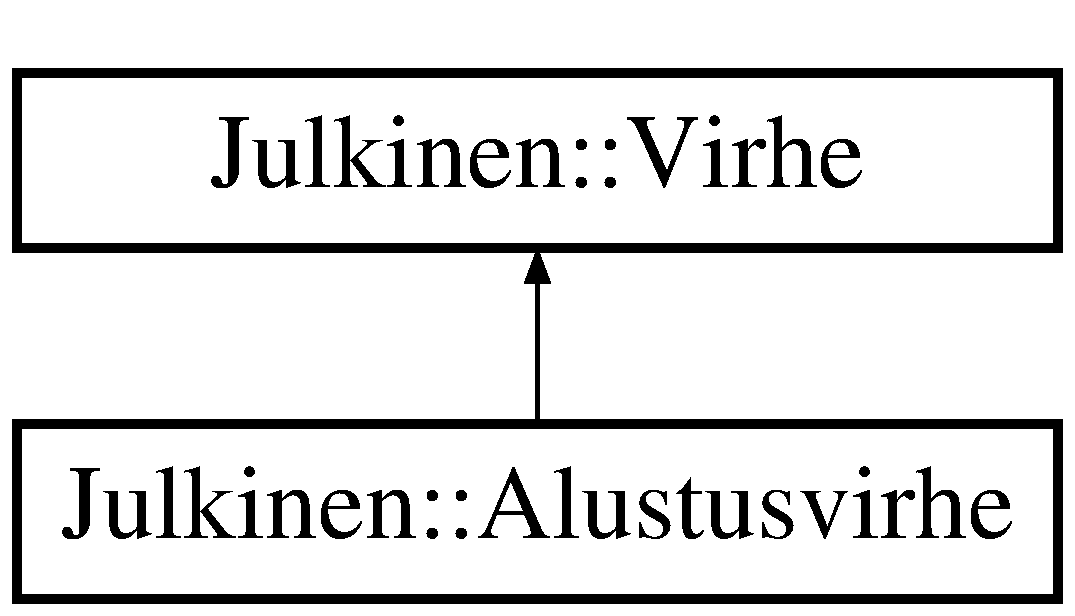
\includegraphics[height=2.000000cm]{class_julkinen_1_1_alustusvirhe}
\end{center}
\end{figure}
\subsection*{Public Types}
\begin{DoxyCompactItemize}
\item 
enum \hyperlink{class_julkinen_1_1_alustusvirhe_a6c27ff51ee369cf37028b8a7ea0eafc0}{Virhekoodi} \{ \\*
\hyperlink{class_julkinen_1_1_alustusvirhe_a6c27ff51ee369cf37028b8a7ea0eafc0aec9736ad2af67e08e50b87117617f4d6}{V\+I\+R\+H\+E\+\_\+\+P\+A\+L\+A\+S\+S\+A\+\_\+\+O\+N\+\_\+\+J\+O\+\_\+\+E\+S\+I\+N\+E}, 
\hyperlink{class_julkinen_1_1_alustusvirhe_a6c27ff51ee369cf37028b8a7ea0eafc0a733522f56cfb8984ea41adc51baf8741}{V\+I\+R\+H\+E\+E\+L\+L\+I\+N\+E\+N\+\_\+\+S\+I\+J\+A\+I\+N\+T\+I}, 
\hyperlink{class_julkinen_1_1_alustusvirhe_a6c27ff51ee369cf37028b8a7ea0eafc0ac9bd1b203cef3970b61807a7c8d1e004}{V\+I\+R\+H\+E\+E\+L\+L\+I\+N\+E\+N\+\_\+\+R\+O\+T\+A\+A\+T\+I\+O}, 
{\bfseries V\+I\+R\+H\+E\+\_\+\+A\+N\+N\+E\+T\+T\+U\+A\+\_\+\+P\+E\+L\+A\+A\+J\+A\+A\+\_\+\+E\+I\+\_\+\+L\+O\+Y\+T\+Y\+N\+Y\+T}, 
\\*
{\bfseries V\+I\+R\+H\+E\+\_\+\+L\+I\+I\+K\+A\+A\+\_\+\+P\+A\+R\+A\+M\+E\+T\+R\+E\+J\+A}, 
\hyperlink{class_julkinen_1_1_alustusvirhe_a6c27ff51ee369cf37028b8a7ea0eafc0a37797a3ef54020c869caea8d10b51e46}{V\+I\+R\+H\+E\+\_\+\+T\+U\+N\+N\+I\+S\+T\+A\+M\+A\+T\+O\+N}
 \}\begin{DoxyCompactList}\small\item\em Tunnisteet esimääritellyille virhetilanteille käyttäjän antamissa komennoissa. \end{DoxyCompactList}
\end{DoxyCompactItemize}
\subsection*{Public Member Functions}
\begin{DoxyCompactItemize}
\item 
\hyperlink{class_julkinen_1_1_alustusvirhe_aab6d2164d8c55d404febff382556a8fd}{Alustusvirhe} (std\+::string const \&virheviesti)
\begin{DoxyCompactList}\small\item\em Tunnistamaton virhetilanne kopioidulla viestillä. \end{DoxyCompactList}\item 
\hyperlink{class_julkinen_1_1_alustusvirhe_a46f9b253c9ce0336c12bad1d2f3a93a1}{Alustusvirhe} (\hyperlink{class_julkinen_1_1_alustusvirhe_a6c27ff51ee369cf37028b8a7ea0eafc0}{Julkinen\+::\+Alustusvirhe\+::\+Virhekoodi} virhekoodi)
\begin{DoxyCompactList}\small\item\em Esimääritelty virhetilanne. \end{DoxyCompactList}\item 
\hyperlink{class_julkinen_1_1_alustusvirhe_a03dbadc97b43077338d874c899c9da1d}{Alustusvirhe} (\hyperlink{class_julkinen_1_1_alustusvirhe}{Julkinen\+::\+Alustusvirhe} const \&toinen)
\begin{DoxyCompactList}\small\item\em Kopiorakentaja. \end{DoxyCompactList}\item 
\hyperlink{class_julkinen_1_1_alustusvirhe}{Alustusvirhe} \& \hyperlink{class_julkinen_1_1_alustusvirhe_a520656e118da9c9e7baf1baeeacb972e}{operator=} (\hyperlink{class_julkinen_1_1_alustusvirhe}{Julkinen\+::\+Alustusvirhe} const \&toinen)
\begin{DoxyCompactList}\small\item\em Sijoitusoperaattori. \end{DoxyCompactList}\item 
\hypertarget{class_julkinen_1_1_alustusvirhe_af9a610132f2dccefe4b3ba2bf241cd2d}{}\hyperlink{class_julkinen_1_1_alustusvirhe_a6c27ff51ee369cf37028b8a7ea0eafc0}{Virhekoodi} \hyperlink{class_julkinen_1_1_alustusvirhe_af9a610132f2dccefe4b3ba2bf241cd2d}{virhe} () const \label{class_julkinen_1_1_alustusvirhe_af9a610132f2dccefe4b3ba2bf241cd2d}

\begin{DoxyCompactList}\small\item\em Sattuneen virhetilanteen virhekoodi. \end{DoxyCompactList}\item 
virtual std\+::basic\+\_\+ostream$<$ char $>$ \& \hyperlink{class_julkinen_1_1_alustusvirhe_a22b50252a516b339d126261978fb62c1}{tulosta} (std\+::basic\+\_\+ostream$<$ char $>$ \&tuloste) const 
\begin{DoxyCompactList}\small\item\em Tulosta virheen viesti virtaan. \end{DoxyCompactList}\end{DoxyCompactItemize}
\subsection*{Additional Inherited Members}


\subsection{Detailed Description}
Alustuksessa tapahtuvaa virhettä kuvaava poikkeus. 

\subsection{Member Enumeration Documentation}
\hypertarget{class_julkinen_1_1_alustusvirhe_a6c27ff51ee369cf37028b8a7ea0eafc0}{}\index{Julkinen\+::\+Alustusvirhe@{Julkinen\+::\+Alustusvirhe}!Virhekoodi@{Virhekoodi}}
\index{Virhekoodi@{Virhekoodi}!Julkinen\+::\+Alustusvirhe@{Julkinen\+::\+Alustusvirhe}}
\subsubsection[{Virhekoodi}]{\setlength{\rightskip}{0pt plus 5cm}enum {\bf Julkinen\+::\+Alustusvirhe\+::\+Virhekoodi}}\label{class_julkinen_1_1_alustusvirhe_a6c27ff51ee369cf37028b8a7ea0eafc0}


Tunnisteet esimääritellyille virhetilanteille käyttäjän antamissa komennoissa. 

\begin{Desc}
\item[Enumerator]\par
\begin{description}
\index{V\+I\+R\+H\+E\+\_\+\+P\+A\+L\+A\+S\+S\+A\+\_\+\+O\+N\+\_\+\+J\+O\+\_\+\+E\+S\+I\+N\+E@{V\+I\+R\+H\+E\+\_\+\+P\+A\+L\+A\+S\+S\+A\+\_\+\+O\+N\+\_\+\+J\+O\+\_\+\+E\+S\+I\+N\+E}!Julkinen\+::\+Alustusvirhe@{Julkinen\+::\+Alustusvirhe}}\index{Julkinen\+::\+Alustusvirhe@{Julkinen\+::\+Alustusvirhe}!V\+I\+R\+H\+E\+\_\+\+P\+A\+L\+A\+S\+S\+A\+\_\+\+O\+N\+\_\+\+J\+O\+\_\+\+E\+S\+I\+N\+E@{V\+I\+R\+H\+E\+\_\+\+P\+A\+L\+A\+S\+S\+A\+\_\+\+O\+N\+\_\+\+J\+O\+\_\+\+E\+S\+I\+N\+E}}\item[{\em 
\hypertarget{class_julkinen_1_1_alustusvirhe_a6c27ff51ee369cf37028b8a7ea0eafc0aec9736ad2af67e08e50b87117617f4d6}{}V\+I\+R\+H\+E\+\_\+\+P\+A\+L\+A\+S\+S\+A\+\_\+\+O\+N\+\_\+\+J\+O\+\_\+\+E\+S\+I\+N\+E\label{class_julkinen_1_1_alustusvirhe_a6c27ff51ee369cf37028b8a7ea0eafc0aec9736ad2af67e08e50b87117617f4d6}
}]Irtopala on jo työnnetty tällä vuorolla ja pelaaja yrittää työntää sitä uudestaan. \index{V\+I\+R\+H\+E\+E\+L\+L\+I\+N\+E\+N\+\_\+\+S\+I\+J\+A\+I\+N\+T\+I@{V\+I\+R\+H\+E\+E\+L\+L\+I\+N\+E\+N\+\_\+\+S\+I\+J\+A\+I\+N\+T\+I}!Julkinen\+::\+Alustusvirhe@{Julkinen\+::\+Alustusvirhe}}\index{Julkinen\+::\+Alustusvirhe@{Julkinen\+::\+Alustusvirhe}!V\+I\+R\+H\+E\+E\+L\+L\+I\+N\+E\+N\+\_\+\+S\+I\+J\+A\+I\+N\+T\+I@{V\+I\+R\+H\+E\+E\+L\+L\+I\+N\+E\+N\+\_\+\+S\+I\+J\+A\+I\+N\+T\+I}}\item[{\em 
\hypertarget{class_julkinen_1_1_alustusvirhe_a6c27ff51ee369cf37028b8a7ea0eafc0a733522f56cfb8984ea41adc51baf8741}{}V\+I\+R\+H\+E\+E\+L\+L\+I\+N\+E\+N\+\_\+\+S\+I\+J\+A\+I\+N\+T\+I\label{class_julkinen_1_1_alustusvirhe_a6c27ff51ee369cf37028b8a7ea0eafc0a733522f56cfb8984ea41adc51baf8741}
}]Annettu sijainti on virheellinen. \index{V\+I\+R\+H\+E\+E\+L\+L\+I\+N\+E\+N\+\_\+\+R\+O\+T\+A\+A\+T\+I\+O@{V\+I\+R\+H\+E\+E\+L\+L\+I\+N\+E\+N\+\_\+\+R\+O\+T\+A\+A\+T\+I\+O}!Julkinen\+::\+Alustusvirhe@{Julkinen\+::\+Alustusvirhe}}\index{Julkinen\+::\+Alustusvirhe@{Julkinen\+::\+Alustusvirhe}!V\+I\+R\+H\+E\+E\+L\+L\+I\+N\+E\+N\+\_\+\+R\+O\+T\+A\+A\+T\+I\+O@{V\+I\+R\+H\+E\+E\+L\+L\+I\+N\+E\+N\+\_\+\+R\+O\+T\+A\+A\+T\+I\+O}}\item[{\em 
\hypertarget{class_julkinen_1_1_alustusvirhe_a6c27ff51ee369cf37028b8a7ea0eafc0ac9bd1b203cef3970b61807a7c8d1e004}{}V\+I\+R\+H\+E\+E\+L\+L\+I\+N\+E\+N\+\_\+\+R\+O\+T\+A\+A\+T\+I\+O\label{class_julkinen_1_1_alustusvirhe_a6c27ff51ee369cf37028b8a7ea0eafc0ac9bd1b203cef3970b61807a7c8d1e004}
}]Annettu rotaatio on virheellinen. \index{V\+I\+R\+H\+E\+\_\+\+T\+U\+N\+N\+I\+S\+T\+A\+M\+A\+T\+O\+N@{V\+I\+R\+H\+E\+\_\+\+T\+U\+N\+N\+I\+S\+T\+A\+M\+A\+T\+O\+N}!Julkinen\+::\+Alustusvirhe@{Julkinen\+::\+Alustusvirhe}}\index{Julkinen\+::\+Alustusvirhe@{Julkinen\+::\+Alustusvirhe}!V\+I\+R\+H\+E\+\_\+\+T\+U\+N\+N\+I\+S\+T\+A\+M\+A\+T\+O\+N@{V\+I\+R\+H\+E\+\_\+\+T\+U\+N\+N\+I\+S\+T\+A\+M\+A\+T\+O\+N}}\item[{\em 
\hypertarget{class_julkinen_1_1_alustusvirhe_a6c27ff51ee369cf37028b8a7ea0eafc0a37797a3ef54020c869caea8d10b51e46}{}V\+I\+R\+H\+E\+\_\+\+T\+U\+N\+N\+I\+S\+T\+A\+M\+A\+T\+O\+N\label{class_julkinen_1_1_alustusvirhe_a6c27ff51ee369cf37028b8a7ea0eafc0a37797a3ef54020c869caea8d10b51e46}
}]Tunnistamaton virhe. \end{description}
\end{Desc}


\subsection{Constructor \& Destructor Documentation}
\hypertarget{class_julkinen_1_1_alustusvirhe_aab6d2164d8c55d404febff382556a8fd}{}\index{Julkinen\+::\+Alustusvirhe@{Julkinen\+::\+Alustusvirhe}!Alustusvirhe@{Alustusvirhe}}
\index{Alustusvirhe@{Alustusvirhe}!Julkinen\+::\+Alustusvirhe@{Julkinen\+::\+Alustusvirhe}}
\subsubsection[{Alustusvirhe(std\+::string const \&virheviesti)}]{\setlength{\rightskip}{0pt plus 5cm}Alustusvirhe\+::\+Alustusvirhe (
\begin{DoxyParamCaption}
\item[{std\+::string const \&}]{virheviesti}
\end{DoxyParamCaption}
)\hspace{0.3cm}{\ttfamily [explicit]}}\label{class_julkinen_1_1_alustusvirhe_aab6d2164d8c55d404febff382556a8fd}


Tunnistamaton virhetilanne kopioidulla viestillä. 

Käytä tätä vain, jos kyseessä ei ole mikään esimääritellyistä virheistä.

\begin{DoxyPostcond}{Postcondition}
Perustakuu poikkeuksen sattuessa. 
\end{DoxyPostcond}

\begin{DoxyParams}{Parameters}
{\em virheviesti} & Merkkijono, joka kopioidaan poikkeuksen viestiksi. \\
\hline
\end{DoxyParams}

\begin{DoxyExceptions}{Exceptions}
{\em std\+::bad\+\_\+alloc} & Ei saatu varattua muistia viestiä varten. \\
\hline
\end{DoxyExceptions}
\hypertarget{class_julkinen_1_1_alustusvirhe_a46f9b253c9ce0336c12bad1d2f3a93a1}{}\index{Julkinen\+::\+Alustusvirhe@{Julkinen\+::\+Alustusvirhe}!Alustusvirhe@{Alustusvirhe}}
\index{Alustusvirhe@{Alustusvirhe}!Julkinen\+::\+Alustusvirhe@{Julkinen\+::\+Alustusvirhe}}
\subsubsection[{Alustusvirhe(\+Julkinen\+::\+Alustusvirhe\+::\+Virhekoodi virhekoodi)}]{\setlength{\rightskip}{0pt plus 5cm}Alustusvirhe\+::\+Alustusvirhe (
\begin{DoxyParamCaption}
\item[{{\bf Julkinen\+::\+Alustusvirhe\+::\+Virhekoodi}}]{virhekoodi}
\end{DoxyParamCaption}
)\hspace{0.3cm}{\ttfamily [explicit]}}\label{class_julkinen_1_1_alustusvirhe_a46f9b253c9ce0336c12bad1d2f3a93a1}


Esimääritelty virhetilanne. 

\begin{DoxyPostcond}{Postcondition}
No-\/throw -\/takuu. 
\end{DoxyPostcond}

\begin{DoxyParams}{Parameters}
{\em virhekoodi} & Virhetilanteen tunniste. Mikäli koodi on V\+I\+R\+H\+E\+\_\+\+T\+U\+N\+N\+I\+S\+T\+A\+M\+A\+T\+O\+N, tulee viestiksi \char`\"{}\+Tunnistamaton virhe.\char`\"{}. \\
\hline
\end{DoxyParams}
\hypertarget{class_julkinen_1_1_alustusvirhe_a03dbadc97b43077338d874c899c9da1d}{}\index{Julkinen\+::\+Alustusvirhe@{Julkinen\+::\+Alustusvirhe}!Alustusvirhe@{Alustusvirhe}}
\index{Alustusvirhe@{Alustusvirhe}!Julkinen\+::\+Alustusvirhe@{Julkinen\+::\+Alustusvirhe}}
\subsubsection[{Alustusvirhe(\+Julkinen\+::\+Alustusvirhe const \&toinen)}]{\setlength{\rightskip}{0pt plus 5cm}Alustusvirhe\+::\+Alustusvirhe (
\begin{DoxyParamCaption}
\item[{{\bf Julkinen\+::\+Alustusvirhe} const \&}]{toinen}
\end{DoxyParamCaption}
)}\label{class_julkinen_1_1_alustusvirhe_a03dbadc97b43077338d874c899c9da1d}


Kopiorakentaja. 

\begin{DoxyPostcond}{Postcondition}
No-\/throw -\/takuu. 
\end{DoxyPostcond}


\subsection{Member Function Documentation}
\hypertarget{class_julkinen_1_1_alustusvirhe_a520656e118da9c9e7baf1baeeacb972e}{}\index{Julkinen\+::\+Alustusvirhe@{Julkinen\+::\+Alustusvirhe}!operator=@{operator=}}
\index{operator=@{operator=}!Julkinen\+::\+Alustusvirhe@{Julkinen\+::\+Alustusvirhe}}
\subsubsection[{operator=(\+Julkinen\+::\+Alustusvirhe const \&toinen)}]{\setlength{\rightskip}{0pt plus 5cm}{\bf Alustusvirhe} \& Alustusvirhe\+::operator= (
\begin{DoxyParamCaption}
\item[{{\bf Julkinen\+::\+Alustusvirhe} const \&}]{toinen}
\end{DoxyParamCaption}
)}\label{class_julkinen_1_1_alustusvirhe_a520656e118da9c9e7baf1baeeacb972e}


Sijoitusoperaattori. 

\begin{DoxyPostcond}{Postcondition}
No-\/throw -\/takuu. 
\end{DoxyPostcond}
\hypertarget{class_julkinen_1_1_alustusvirhe_a22b50252a516b339d126261978fb62c1}{}\index{Julkinen\+::\+Alustusvirhe@{Julkinen\+::\+Alustusvirhe}!tulosta@{tulosta}}
\index{tulosta@{tulosta}!Julkinen\+::\+Alustusvirhe@{Julkinen\+::\+Alustusvirhe}}
\subsubsection[{tulosta(std\+::basic\+\_\+ostream$<$ char $>$ \&tuloste) const }]{\setlength{\rightskip}{0pt plus 5cm}basic\+\_\+ostream$<$ char $>$ \& Alustusvirhe\+::tulosta (
\begin{DoxyParamCaption}
\item[{std\+::basic\+\_\+ostream$<$ char $>$ \&}]{tuloste}
\end{DoxyParamCaption}
) const\hspace{0.3cm}{\ttfamily [virtual]}}\label{class_julkinen_1_1_alustusvirhe_a22b50252a516b339d126261978fb62c1}


Tulosta virheen viesti virtaan. 

Tulostaa virheen viestin virtaan, eikä tee muuta.

\begin{DoxyPostcond}{Postcondition}
Vahva poikkeustakuu. 
\end{DoxyPostcond}

\begin{DoxyParams}{Parameters}
{\em tuloste} & Virta, jonne viesti tulostetaan. \\
\hline
\end{DoxyParams}
\begin{DoxyReturn}{Returns}
{\ttfamily tuloste} 
\end{DoxyReturn}


Reimplemented from \hyperlink{class_julkinen_1_1_virhe_a36a2644943038f9760b5d76a1960b00d}{Julkinen\+::\+Virhe}.



The documentation for this class was generated from the following files\+:\begin{DoxyCompactItemize}
\item 
\hyperlink{alustusvirhe_8hh}{alustusvirhe.\+hh}\item 
valmiiden\+\_\+toteutus/\hyperlink{alustusvirhe_8cc}{alustusvirhe.\+cc}\end{DoxyCompactItemize}

\hypertarget{class_bittikartta}{}\section{Bittikartta Class Reference}
\label{class_bittikartta}\index{Bittikartta@{Bittikartta}}


{\ttfamily \#include $<$Bittikartta.\+hh$>$}

\subsection*{Public Member Functions}
\begin{DoxyCompactItemize}
\item 
\hyperlink{class_bittikartta_a6ba90dfc35beaace33ed8db98138f938}{Bittikartta} (\hyperlink{_bittikartta_8hh_a3de8ab5c710592d442741fc105c483aa}{Dim} leveys, \hyperlink{_bittikartta_8hh_a3de8ab5c710592d442741fc105c483aa}{Dim} korkeus)
\item 
\hyperlink{class_bittikartta_a633060ae1338842a3d175cae80a9fde6}{$\sim$\+Bittikartta} ()
\item 
void \hyperlink{class_bittikartta_a139d5c1072e015fbf1ef6d283b278e77}{vaakateksti} (\hyperlink{_bittikartta_8hh_a3de8ab5c710592d442741fc105c483aa}{Dim} x, \hyperlink{_bittikartta_8hh_a3de8ab5c710592d442741fc105c483aa}{Dim} y, std\+::string const \&teksti)
\item 
void \hyperlink{class_bittikartta_a7886d157f711dec0b44fdbc9a9a5ee92}{pystyteksti} (\hyperlink{_bittikartta_8hh_a3de8ab5c710592d442741fc105c483aa}{Dim} x, \hyperlink{_bittikartta_8hh_a3de8ab5c710592d442741fc105c483aa}{Dim} y, std\+::string const \&teksti)
\item 
void \hyperlink{class_bittikartta_a3c01a7b0f71cc48899b1a300c3f5dfb9}{suorakaide} (\hyperlink{_bittikartta_8hh_a3de8ab5c710592d442741fc105c483aa}{Dim} x, \hyperlink{_bittikartta_8hh_a3de8ab5c710592d442741fc105c483aa}{Dim} y, \hyperlink{_bittikartta_8hh_a3de8ab5c710592d442741fc105c483aa}{Dim} lev, \hyperlink{_bittikartta_8hh_a3de8ab5c710592d442741fc105c483aa}{Dim} kork, char merkki)
\item 
void \hyperlink{class_bittikartta_acb0ee37ce104c9337233896b5f157063}{tyhjenna} ()
\item 
void \hyperlink{class_bittikartta_a484bf5feefcc803a039937c704f34a17}{tulosta} (std\+::ostream \&virta) const 
\item 
void \hyperlink{class_bittikartta_a063f6631901b378de7d5212683ed15a0}{vaakaviiva} (\hyperlink{_bittikartta_8hh_a3de8ab5c710592d442741fc105c483aa}{Dim} x, \hyperlink{_bittikartta_8hh_a3de8ab5c710592d442741fc105c483aa}{Dim} y, \hyperlink{_bittikartta_8hh_a3de8ab5c710592d442741fc105c483aa}{Dim} lev, char merkki)
\item 
void \hyperlink{class_bittikartta_a134b78d3c6cf7be361bfdebbd297787a}{pystyviiva} (\hyperlink{_bittikartta_8hh_a3de8ab5c710592d442741fc105c483aa}{Dim} x, \hyperlink{_bittikartta_8hh_a3de8ab5c710592d442741fc105c483aa}{Dim} y, \hyperlink{_bittikartta_8hh_a3de8ab5c710592d442741fc105c483aa}{Dim} kork, char merkki)
\end{DoxyCompactItemize}


\subsection{Detailed Description}
Bittikartta-\/luokka mahdollistaa tulostusten tekemisen vaiheittain Bittikartta-\/luokan olioon ja vasta lopuksi tulostamisen ruudulle.

{\bfseries Huom!} Bittikartta-\/luokan origo (0,0) on {\itshape vasemmassa yl�nurkassa} ja y-\/suunta kasvaa alasp�in. 

\subsection{Constructor \& Destructor Documentation}
\hypertarget{class_bittikartta_a6ba90dfc35beaace33ed8db98138f938}{}\index{Bittikartta@{Bittikartta}!Bittikartta@{Bittikartta}}
\index{Bittikartta@{Bittikartta}!Bittikartta@{Bittikartta}}
\subsubsection[{Bittikartta(\+Dim leveys, Dim korkeus)}]{\setlength{\rightskip}{0pt plus 5cm}Bittikartta\+::\+Bittikartta (
\begin{DoxyParamCaption}
\item[{{\bf Dim}}]{leveys, }
\item[{{\bf Dim}}]{korkeus}
\end{DoxyParamCaption}
)}\label{class_bittikartta_a6ba90dfc35beaace33ed8db98138f938}

\begin{DoxyParams}{Parameters}
{\em leveys} & piirtoalueen leveys \\
\hline
{\em korkeus} & piirtoalueen korkeus \\
\hline
\end{DoxyParams}
\hypertarget{class_bittikartta_a633060ae1338842a3d175cae80a9fde6}{}\index{Bittikartta@{Bittikartta}!````~Bittikartta@{$\sim$\+Bittikartta}}
\index{````~Bittikartta@{$\sim$\+Bittikartta}!Bittikartta@{Bittikartta}}
\subsubsection[{$\sim$\+Bittikartta()}]{\setlength{\rightskip}{0pt plus 5cm}Bittikartta\+::$\sim$\+Bittikartta (
\begin{DoxyParamCaption}
{}
\end{DoxyParamCaption}
)}\label{class_bittikartta_a633060ae1338842a3d175cae80a9fde6}
Purkaja 

\subsection{Member Function Documentation}
\hypertarget{class_bittikartta_a7886d157f711dec0b44fdbc9a9a5ee92}{}\index{Bittikartta@{Bittikartta}!pystyteksti@{pystyteksti}}
\index{pystyteksti@{pystyteksti}!Bittikartta@{Bittikartta}}
\subsubsection[{pystyteksti(\+Dim x, Dim y, std\+::string const \&teksti)}]{\setlength{\rightskip}{0pt plus 5cm}void Bittikartta\+::pystyteksti (
\begin{DoxyParamCaption}
\item[{{\bf Dim}}]{x, }
\item[{{\bf Dim}}]{y, }
\item[{std\+::string const \&}]{teksti}
\end{DoxyParamCaption}
)}\label{class_bittikartta_a7886d157f711dec0b44fdbc9a9a5ee92}
Kirjoittaa alueelle pystytekstin, joka alkaa koordinaateista (x, y). Viimeinen merkki tulee pisteeseen (x, y + tekstin pituus). Bittikartta-\/luokan origo (0,0) on {\itshape vasemmassa yl�nurkassa} ja y-\/suunta kasvaa alasp�in. 
\begin{DoxyParams}{Parameters}
{\em x} & alkupisteen x-\/koordinaatti \\
\hline
{\em y} & alkupisteen y-\/koordinaatti \\
\hline
{\em teksti} & kirjoitettava teksti \\
\hline
\end{DoxyParams}
\hypertarget{class_bittikartta_a134b78d3c6cf7be361bfdebbd297787a}{}\index{Bittikartta@{Bittikartta}!pystyviiva@{pystyviiva}}
\index{pystyviiva@{pystyviiva}!Bittikartta@{Bittikartta}}
\subsubsection[{pystyviiva(\+Dim x, Dim y, Dim kork, char merkki)}]{\setlength{\rightskip}{0pt plus 5cm}void Bittikartta\+::pystyviiva (
\begin{DoxyParamCaption}
\item[{{\bf Dim}}]{x, }
\item[{{\bf Dim}}]{y, }
\item[{{\bf Dim}}]{kork, }
\item[{char}]{merkki}
\end{DoxyParamCaption}
)}\label{class_bittikartta_a134b78d3c6cf7be361bfdebbd297787a}
Piirt�� vertikaalisen viivan eli pystyviivan. Bittikartta-\/luokan origo (0,0) on {\itshape vasemmassa yl�nurkassa} ja y-\/suunta kasvaa alasp�in. 
\begin{DoxyParams}{Parameters}
{\em x} & alkupisteen x-\/koordinaatti \\
\hline
{\em y} & alkupisteen y-\/koordinaatti \\
\hline
{\em kork} & viivan korkeus \\
\hline
{\em merkki} & viivan piirtoon k�ytett�v� merkki \\
\hline
\end{DoxyParams}
\hypertarget{class_bittikartta_a3c01a7b0f71cc48899b1a300c3f5dfb9}{}\index{Bittikartta@{Bittikartta}!suorakaide@{suorakaide}}
\index{suorakaide@{suorakaide}!Bittikartta@{Bittikartta}}
\subsubsection[{suorakaide(\+Dim x, Dim y, Dim lev, Dim kork, char merkki)}]{\setlength{\rightskip}{0pt plus 5cm}void Bittikartta\+::suorakaide (
\begin{DoxyParamCaption}
\item[{{\bf Dim}}]{x, }
\item[{{\bf Dim}}]{y, }
\item[{{\bf Dim}}]{lev, }
\item[{{\bf Dim}}]{kork, }
\item[{char}]{merkki}
\end{DoxyParamCaption}
)}\label{class_bittikartta_a3c01a7b0f71cc48899b1a300c3f5dfb9}
Piirt�� suorakaiteen, jonka vasen yl�kulma on pisteess� (x, y). Reunat piirret��n annetulla merkill�. Bittikartta-\/luokan origo (0,0) on {\itshape vasemmassa yl�nurkassa} ja y-\/suunta kasvaa alasp�in. 
\begin{DoxyParams}{Parameters}
{\em x} & alkupisteen x-\/koordinaatti \\
\hline
{\em y} & alkupisteen y-\/koordinaatti \\
\hline
{\em lev} & suorakaiteen leveys \\
\hline
{\em kork} & suorakaiteen korkeus \\
\hline
{\em merkki} & alueen ��riviivojen piirt�miseen k�ytett�v� merkki \\
\hline
\end{DoxyParams}
\hypertarget{class_bittikartta_a484bf5feefcc803a039937c704f34a17}{}\index{Bittikartta@{Bittikartta}!tulosta@{tulosta}}
\index{tulosta@{tulosta}!Bittikartta@{Bittikartta}}
\subsubsection[{tulosta(std\+::ostream \&virta) const }]{\setlength{\rightskip}{0pt plus 5cm}void Bittikartta\+::tulosta (
\begin{DoxyParamCaption}
\item[{std\+::ostream \&}]{virta}
\end{DoxyParamCaption}
) const}\label{class_bittikartta_a484bf5feefcc803a039937c704f34a17}
Tulostaa bittikartan sis�ll�n annettuun virtaan. 
\begin{DoxyParams}{Parameters}
{\em virta} & virta, johon bittikartta tulostetaan \\
\hline
\end{DoxyParams}
\hypertarget{class_bittikartta_acb0ee37ce104c9337233896b5f157063}{}\index{Bittikartta@{Bittikartta}!tyhjenna@{tyhjenna}}
\index{tyhjenna@{tyhjenna}!Bittikartta@{Bittikartta}}
\subsubsection[{tyhjenna()}]{\setlength{\rightskip}{0pt plus 5cm}void Bittikartta\+::tyhjenna (
\begin{DoxyParamCaption}
{}
\end{DoxyParamCaption}
)}\label{class_bittikartta_acb0ee37ce104c9337233896b5f157063}
Pyyhkii piirtoalueen eli korvaa kaikki piirretyt merkit v�lily�nneill�. \hypertarget{class_bittikartta_a139d5c1072e015fbf1ef6d283b278e77}{}\index{Bittikartta@{Bittikartta}!vaakateksti@{vaakateksti}}
\index{vaakateksti@{vaakateksti}!Bittikartta@{Bittikartta}}
\subsubsection[{vaakateksti(\+Dim x, Dim y, std\+::string const \&teksti)}]{\setlength{\rightskip}{0pt plus 5cm}void Bittikartta\+::vaakateksti (
\begin{DoxyParamCaption}
\item[{{\bf Dim}}]{x, }
\item[{{\bf Dim}}]{y, }
\item[{std\+::string const \&}]{teksti}
\end{DoxyParamCaption}
)}\label{class_bittikartta_a139d5c1072e015fbf1ef6d283b278e77}
Kirjoittaa alueelle vaakatekstin, joka alkaa koordinaateista (x, y). Viimeinen merkki tulee pisteeseen (x + tekstin pituus, y). Bittikartta-\/luokan origo (0,0) on {\itshape vasemmassa yl�nurkassa} ja y-\/suunta kasvaa alasp�in. 
\begin{DoxyParams}{Parameters}
{\em x} & alkupisteen x-\/koordinaatti \\
\hline
{\em y} & alkupisteen y-\/koordinaatti \\
\hline
{\em teksti} & kirjoitettava teksti \\
\hline
\end{DoxyParams}
\hypertarget{class_bittikartta_a063f6631901b378de7d5212683ed15a0}{}\index{Bittikartta@{Bittikartta}!vaakaviiva@{vaakaviiva}}
\index{vaakaviiva@{vaakaviiva}!Bittikartta@{Bittikartta}}
\subsubsection[{vaakaviiva(\+Dim x, Dim y, Dim lev, char merkki)}]{\setlength{\rightskip}{0pt plus 5cm}void Bittikartta\+::vaakaviiva (
\begin{DoxyParamCaption}
\item[{{\bf Dim}}]{x, }
\item[{{\bf Dim}}]{y, }
\item[{{\bf Dim}}]{lev, }
\item[{char}]{merkki}
\end{DoxyParamCaption}
)}\label{class_bittikartta_a063f6631901b378de7d5212683ed15a0}
Piirt�� horisontaalisen viivan eli vaakaviivan. Bittikartta-\/luokan origo (0,0) on {\itshape vasemmassa yl�nurkassa} ja y-\/suunta kasvaa alasp�in. 
\begin{DoxyParams}{Parameters}
{\em x} & alkupisteen x-\/koordinaatti \\
\hline
{\em y} & alkupisteen y-\/koordinaatti \\
\hline
{\em lev} & viivan leveys \\
\hline
{\em merkki} & viivan piirtoon k�ytett�v� merkki \\
\hline
\end{DoxyParams}


The documentation for this class was generated from the following files\+:\begin{DoxyCompactItemize}
\item 
valmiiden\+\_\+toteutus/include/\hyperlink{_bittikartta_8hh}{Bittikartta.\+hh}\item 
valmiiden\+\_\+toteutus/\hyperlink{_bittikartta_8cc}{Bittikartta.\+cc}\end{DoxyCompactItemize}

\hypertarget{class_data}{}\section{Data Class Reference}
\label{class_data}\index{Data@{Data}}
\subsection*{Public Member Functions}
\begin{DoxyCompactItemize}
\item 
\hyperlink{class_data_af11f741cb7f587e2e495452a8905a22a}{Data} ()
\begin{DoxyCompactList}\small\item\em Datan rakentaja. \end{DoxyCompactList}\item 
\hyperlink{class_data_aab31956423290f0d62dcca47ab4d16dd}{$\sim$\+Data} ()
\begin{DoxyCompactList}\small\item\em Purkaja. \end{DoxyCompactList}\item 
\hyperlink{class_pelaaja}{Pelaaja} $\ast$ \hyperlink{class_data_a6f101f9a140fab0da6bac6dec96e491d}{hae\+Pelaaja} (std\+::string name)
\begin{DoxyCompactList}\small\item\em Pelaajan osoitteen nimestä hakija. \end{DoxyCompactList}\item 
\hyperlink{class_julkinen_1_1_koordinaatti}{Julkinen\+::\+Koordinaatti} \hyperlink{class_data_a8edef6853dc63d894651b5413b9da87b}{hae\+Esine} (char merkki) const 
\begin{DoxyCompactList}\small\item\em Esineen kordinaattien hakija. \end{DoxyCompactList}\item 
\hyperlink{class_esine}{Esine} $\ast$ \hyperlink{class_data_a1d86d15d120a5451f2dfdf2b1644056e}{hae\+Esine} (\hyperlink{class_julkinen_1_1_koordinaatti}{Julkinen\+::\+Koordinaatti} const \&kordinaatit)
\begin{DoxyCompactList}\small\item\em Esineen osoitteen hakija. \end{DoxyCompactList}\item 
\hyperlink{class_pala}{Pala} $\ast$ \hyperlink{class_data_a05494446c31564a36f0b6a09a743420c}{hae\+Pala} (\hyperlink{class_julkinen_1_1_koordinaatti}{Julkinen\+::\+Koordinaatti} const \&kordinaatit)
\begin{DoxyCompactList}\small\item\em Palan osoitteen hakija. \end{DoxyCompactList}\item 
\hyperlink{class_pelaaja}{Pelaaja} $\ast$ \hyperlink{class_data_ac46ff8a55f904bcbabf22861036b27b6}{hae\+Pelaaja} (\hyperlink{class_julkinen_1_1_koordinaatti}{Julkinen\+::\+Koordinaatti} const \&kordinaatit)
\begin{DoxyCompactList}\small\item\em Pelaajan osoitteen hakija. \end{DoxyCompactList}\item 
\hyperlink{class_pala}{Pala} $\ast$ \hyperlink{class_data_af715df1467da7242a96b2b3f1f288216}{hae\+Irtopala} ()
\begin{DoxyCompactList}\small\item\em Irtopalan osoitteen hakija. \end{DoxyCompactList}\item 
\hyperlink{class_julkinen_1_1_koordinaatti}{Julkinen\+::\+Koordinaatti} \hyperlink{class_data_ad409f9569c098e68308efb7dc92395ac}{hae\+Pelaajan\+Sijainti} (\hyperlink{class_pelaaja}{Pelaaja} pelaaja) const 
\begin{DoxyCompactList}\small\item\em Pelaajan sijainnin hakija. \end{DoxyCompactList}\item 
\hyperlink{class_julkinen_1_1_koordinaatti}{Julkinen\+::\+Koordinaatti} \hyperlink{class_data_a0cc383355bf597282393b629646add61}{hae\+Esineen\+Sijainti} (\hyperlink{class_esine}{Esine} esine) const 
\begin{DoxyCompactList}\small\item\em Esineen sijainnin hakija. \end{DoxyCompactList}\item 
std\+::vector$<$ \hyperlink{class_esine}{Esine} $>$ \hyperlink{class_data_ab233c0e1b05e62bb05ac03c44412ded2}{hae\+Kaikki\+Esineet} () const 
\begin{DoxyCompactList}\small\item\em Kaikkien esineiden hakija. \end{DoxyCompactList}\item 
std\+::vector$<$ \hyperlink{class_pala}{Pala} $>$ \hyperlink{class_data_a3eefbad880fce0532156b1606dceb590}{hae\+Kaikki\+Palat} () const 
\begin{DoxyCompactList}\small\item\em Kaikkien palojen hakija. \end{DoxyCompactList}\item 
std\+::vector$<$ \hyperlink{class_pelaaja}{Pelaaja} $>$ \hyperlink{class_data_a2b22700aa0ab25293f1cbe7430bea8c0}{hae\+Kaikki\+Pelaajat} () const 
\begin{DoxyCompactList}\small\item\em Kaikkien pelaajien hakija. \end{DoxyCompactList}\item 
std\+::vector$<$ \hyperlink{class_pala}{Pala} $\ast$ $>$ \hyperlink{class_data_ad4c590c292ffe3c1ab7fd5d7d18d9a03}{hae\+Kaikki\+Pala\+Osoitteet} ()
\begin{DoxyCompactList}\small\item\em Kaikkien palojen osoitteiden hakija. \end{DoxyCompactList}\item 
std\+::vector$<$ \hyperlink{class_pelaaja}{Pelaaja} $\ast$ $>$ \hyperlink{class_data_a74e2cf4cbcff5ea1159b91a2b40819bc}{hae\+Kaikki\+Pelaajat\+Osoitteet} ()
\begin{DoxyCompactList}\small\item\em Kaikkien pelaajien osoitteiden hakija. \end{DoxyCompactList}\item 
\hyperlink{class_pelaaja}{Pelaaja} $\ast$ \hyperlink{class_data_a81cc329ff5e8eda227acebd612147e2e}{lisaa\+Pelaaja} (\hyperlink{class_pelaaja}{Pelaaja} data, \hyperlink{class_julkinen_1_1_koordinaatti}{Julkinen\+::\+Koordinaatti} const \&kordinaatit)
\begin{DoxyCompactList}\small\item\em Pelaajan lisääjä \end{DoxyCompactList}\item 
\hyperlink{class_esine}{Esine} $\ast$ \hyperlink{class_data_ad9d038278b49a80ef5bb571a5eff248f}{lisaa\+Esine} (\hyperlink{class_esine}{Esine} data, \hyperlink{class_julkinen_1_1_koordinaatti}{Julkinen\+::\+Koordinaatti} const \&kordinaatit)
\begin{DoxyCompactList}\small\item\em Esineen lisääjä \end{DoxyCompactList}\item 
\hyperlink{class_pala}{Pala} $\ast$ \hyperlink{class_data_a7d19ebd5e1eb95e001c516ad9807ce74}{lisaa\+Pala} (\hyperlink{class_pala}{Pala} data, bool paivita\+Pala=false)
\begin{DoxyCompactList}\small\item\em Palan lisääjä \end{DoxyCompactList}\item 
\hyperlink{class_pala}{Pala} $\ast$ \hyperlink{class_data_a8d0b2dddb62271a7d69008d19bec6f3b}{lisaa\+Irtopala} (\hyperlink{class_pala}{Pala} data)
\begin{DoxyCompactList}\small\item\em Iropalan lisääjä \end{DoxyCompactList}\item 
bool \hyperlink{class_data_af9fb5d0de7876cc689baf4a396157fd2}{liikuta\+Pelaajaa} (std\+::string nimi, \hyperlink{class_julkinen_1_1_koordinaatti}{Julkinen\+::\+Koordinaatti} const \&kordinaatit)
\begin{DoxyCompactList}\small\item\em Pelaajan liikuttaja. \end{DoxyCompactList}\item 
\hyperlink{class_julkinen_1_1_koordinaatti}{Julkinen\+::\+Koordinaatti} \hyperlink{class_data_a1c6055ce5037e81ca1b7caaa5bb6f6b7}{pelaajan\+Seuraavan\+Esineen\+Sijainti} (const \hyperlink{class_pelaaja}{Pelaaja} pelaaja) const 
\begin{DoxyCompactList}\small\item\em Pelaajan seuraavan haettavan esineen sijainnin hakija. \end{DoxyCompactList}\end{DoxyCompactItemize}


\subsection{Constructor \& Destructor Documentation}
\hypertarget{class_data_af11f741cb7f587e2e495452a8905a22a}{}\index{Data@{Data}!Data@{Data}}
\index{Data@{Data}!Data@{Data}}
\subsubsection[{Data()}]{\setlength{\rightskip}{0pt plus 5cm}Data\+::\+Data (
\begin{DoxyParamCaption}
{}
\end{DoxyParamCaption}
)}\label{class_data_af11f741cb7f587e2e495452a8905a22a}


Datan rakentaja. 

Alustaa muuttujat.

\begin{DoxyPostcond}{Postcondition}
Muuttujat on alustettu. 
\end{DoxyPostcond}
\hypertarget{class_data_aab31956423290f0d62dcca47ab4d16dd}{}\index{Data@{Data}!````~Data@{$\sim$\+Data}}
\index{````~Data@{$\sim$\+Data}!Data@{Data}}
\subsubsection[{$\sim$\+Data()}]{\setlength{\rightskip}{0pt plus 5cm}Data\+::$\sim$\+Data (
\begin{DoxyParamCaption}
{}
\end{DoxyParamCaption}
)}\label{class_data_aab31956423290f0d62dcca47ab4d16dd}


Purkaja. 

\begin{DoxyPostcond}{Postcondition}
No-\/throw takuu. 
\end{DoxyPostcond}


\subsection{Member Function Documentation}
\hypertarget{class_data_a8edef6853dc63d894651b5413b9da87b}{}\index{Data@{Data}!hae\+Esine@{hae\+Esine}}
\index{hae\+Esine@{hae\+Esine}!Data@{Data}}
\subsubsection[{hae\+Esine(char merkki) const }]{\setlength{\rightskip}{0pt plus 5cm}{\bf Julkinen\+::\+Koordinaatti} Data\+::hae\+Esine (
\begin{DoxyParamCaption}
\item[{char}]{merkki}
\end{DoxyParamCaption}
) const}\label{class_data_a8edef6853dc63d894651b5413b9da87b}


Esineen kordinaattien hakija. 

Hakee merkkiä vastaavan {\ttfamily \hyperlink{class_esine}{Esine}}-\/luokan kordinaatit.


\begin{DoxyParams}[1]{Parameters}
\mbox{\tt in}  & {\em merkki} & {\ttfamily Haettavan} esineen merkki.\\
\hline
\end{DoxyParams}
\begin{DoxyPostcond}{Postcondition}
Esineen sijainti on haettu.
\end{DoxyPostcond}
\begin{DoxyReturn}{Returns}
Merkkiä vastaavan {\ttfamily \hyperlink{class_esine}{Esine}}-\/luokan kordinaatit {\ttfamily \hyperlink{class_julkinen_1_1_koordinaatti}{Julkinen\+::\+Koordinaatti}}-\/luokkana. 
\end{DoxyReturn}
\hypertarget{class_data_a1d86d15d120a5451f2dfdf2b1644056e}{}\index{Data@{Data}!hae\+Esine@{hae\+Esine}}
\index{hae\+Esine@{hae\+Esine}!Data@{Data}}
\subsubsection[{hae\+Esine(\+Julkinen\+::\+Koordinaatti const \&kordinaatit)}]{\setlength{\rightskip}{0pt plus 5cm}{\bf Esine} $\ast$ Data\+::hae\+Esine (
\begin{DoxyParamCaption}
\item[{{\bf Julkinen\+::\+Koordinaatti} const \&}]{kordinaatit}
\end{DoxyParamCaption}
)}\label{class_data_a1d86d15d120a5451f2dfdf2b1644056e}


Esineen osoitteen hakija. 

Hakee {\ttfamily \hyperlink{class_julkinen_1_1_koordinaatti}{Julkinen\+::\+Koordinaatti}}-\/luokkaa vastaavan {\ttfamily \hyperlink{class_esine}{Esine}}-\/luokan osoitteen.


\begin{DoxyParams}[1]{Parameters}
\mbox{\tt in}  & {\em kordinaatit} & Haettavan esineen kordinaatit {\ttfamily \hyperlink{class_julkinen_1_1_koordinaatti}{Julkinen\+::\+Koordinaatti}}-\/luokkana.\\
\hline
\end{DoxyParams}
\begin{DoxyPostcond}{Postcondition}
Esineen osoite on haettu.
\end{DoxyPostcond}
\begin{DoxyReturn}{Returns}
Merkkiä vastaavan {\ttfamily \hyperlink{class_esine}{Esine}}-\/luokan osoite. 
\end{DoxyReturn}
\hypertarget{class_data_a0cc383355bf597282393b629646add61}{}\index{Data@{Data}!hae\+Esineen\+Sijainti@{hae\+Esineen\+Sijainti}}
\index{hae\+Esineen\+Sijainti@{hae\+Esineen\+Sijainti}!Data@{Data}}
\subsubsection[{hae\+Esineen\+Sijainti(\+Esine esine) const }]{\setlength{\rightskip}{0pt plus 5cm}{\bf Julkinen\+::\+Koordinaatti} Data\+::hae\+Esineen\+Sijainti (
\begin{DoxyParamCaption}
\item[{{\bf Esine}}]{esine}
\end{DoxyParamCaption}
) const}\label{class_data_a0cc383355bf597282393b629646add61}


Esineen sijainnin hakija. 

Hakee {\ttfamily \hyperlink{class_esine}{Esine}}-\/luokkaa vastaavan {\ttfamily \hyperlink{class_esine}{Esine}}-\/luokan kordinaatit.


\begin{DoxyParams}[1]{Parameters}
\mbox{\tt in}  & {\em esine} & Haettava esine {\ttfamily \hyperlink{class_esine}{Esine}}-\/luokkana.\\
\hline
\end{DoxyParams}
\begin{DoxyPostcond}{Postcondition}
Esineen sijainti on haettu.
\end{DoxyPostcond}
\begin{DoxyReturn}{Returns}
Merkkiä vastaavan {\ttfamily \hyperlink{class_esine}{Esine}}-\/luokan kordinaatit {\ttfamily \hyperlink{class_julkinen_1_1_koordinaatti}{Julkinen\+::\+Koordinaatti}}-\/luokkana. 
\end{DoxyReturn}
\hypertarget{class_data_af715df1467da7242a96b2b3f1f288216}{}\index{Data@{Data}!hae\+Irtopala@{hae\+Irtopala}}
\index{hae\+Irtopala@{hae\+Irtopala}!Data@{Data}}
\subsubsection[{hae\+Irtopala()}]{\setlength{\rightskip}{0pt plus 5cm}{\bf Pala} $\ast$ Data\+::hae\+Irtopala (
\begin{DoxyParamCaption}
{}
\end{DoxyParamCaption}
)}\label{class_data_af715df1467da7242a96b2b3f1f288216}


Irtopalan osoitteen hakija. 

Hakee irtopalan osoitteen.

\begin{DoxyPostcond}{Postcondition}
Irtopalan osoite on haettu.
\end{DoxyPostcond}
\begin{DoxyReturn}{Returns}
Irtopalaksi merkityn {\ttfamily \hyperlink{class_pala}{Pala}}-\/luokan osoite. 
\end{DoxyReturn}
\hypertarget{class_data_ab233c0e1b05e62bb05ac03c44412ded2}{}\index{Data@{Data}!hae\+Kaikki\+Esineet@{hae\+Kaikki\+Esineet}}
\index{hae\+Kaikki\+Esineet@{hae\+Kaikki\+Esineet}!Data@{Data}}
\subsubsection[{hae\+Kaikki\+Esineet() const }]{\setlength{\rightskip}{0pt plus 5cm}std\+::vector$<$ {\bf Esine} $>$ Data\+::hae\+Kaikki\+Esineet (
\begin{DoxyParamCaption}
{}
\end{DoxyParamCaption}
) const}\label{class_data_ab233c0e1b05e62bb05ac03c44412ded2}


Kaikkien esineiden hakija. 

Hakee kaikki pelilaudalla olevat esineet {\ttfamily \hyperlink{class_esine}{Esine}}-\/luokkina.

\begin{DoxyPostcond}{Postcondition}
Kaikki esineet on haettu.
\end{DoxyPostcond}
\begin{DoxyReturn}{Returns}
Vektori joka sisältää kaikki esineet {\ttfamily \hyperlink{class_esine}{Esine}}-\/luokkina. 
\end{DoxyReturn}
\hypertarget{class_data_ad4c590c292ffe3c1ab7fd5d7d18d9a03}{}\index{Data@{Data}!hae\+Kaikki\+Pala\+Osoitteet@{hae\+Kaikki\+Pala\+Osoitteet}}
\index{hae\+Kaikki\+Pala\+Osoitteet@{hae\+Kaikki\+Pala\+Osoitteet}!Data@{Data}}
\subsubsection[{hae\+Kaikki\+Pala\+Osoitteet()}]{\setlength{\rightskip}{0pt plus 5cm}std\+::vector$<$ {\bf Pala} $\ast$ $>$ Data\+::hae\+Kaikki\+Pala\+Osoitteet (
\begin{DoxyParamCaption}
{}
\end{DoxyParamCaption}
)}\label{class_data_ad4c590c292ffe3c1ab7fd5d7d18d9a03}


Kaikkien palojen osoitteiden hakija. 

Hakee kaikki pelilaudalla olevat palat {\ttfamily \hyperlink{class_pala}{Pala}}-\/luokkien osoitteina.

\begin{DoxyPostcond}{Postcondition}
Kaikkien pelaajien osoitteet on haettu.
\end{DoxyPostcond}
\begin{DoxyReturn}{Returns}
Vektori joka sisältää kaikki palat {\ttfamily \hyperlink{class_pala}{Pala}}-\/luokan osoitteina. 
\end{DoxyReturn}
\hypertarget{class_data_a3eefbad880fce0532156b1606dceb590}{}\index{Data@{Data}!hae\+Kaikki\+Palat@{hae\+Kaikki\+Palat}}
\index{hae\+Kaikki\+Palat@{hae\+Kaikki\+Palat}!Data@{Data}}
\subsubsection[{hae\+Kaikki\+Palat() const }]{\setlength{\rightskip}{0pt plus 5cm}std\+::vector$<$ {\bf Pala} $>$ Data\+::hae\+Kaikki\+Palat (
\begin{DoxyParamCaption}
{}
\end{DoxyParamCaption}
) const}\label{class_data_a3eefbad880fce0532156b1606dceb590}


Kaikkien palojen hakija. 

Hakee kaikki pelilaudalla olevat palat {\ttfamily \hyperlink{class_pala}{Pala}}-\/luokkina.

\begin{DoxyPostcond}{Postcondition}
Kaikki palat on haettu.
\end{DoxyPostcond}
\begin{DoxyReturn}{Returns}
Vektori joka sisältää kaikki palat {\ttfamily \hyperlink{class_pala}{Pala}}-\/luokkina. 
\end{DoxyReturn}
\hypertarget{class_data_a2b22700aa0ab25293f1cbe7430bea8c0}{}\index{Data@{Data}!hae\+Kaikki\+Pelaajat@{hae\+Kaikki\+Pelaajat}}
\index{hae\+Kaikki\+Pelaajat@{hae\+Kaikki\+Pelaajat}!Data@{Data}}
\subsubsection[{hae\+Kaikki\+Pelaajat() const }]{\setlength{\rightskip}{0pt plus 5cm}std\+::vector$<$ {\bf Pelaaja} $>$ Data\+::hae\+Kaikki\+Pelaajat (
\begin{DoxyParamCaption}
{}
\end{DoxyParamCaption}
) const}\label{class_data_a2b22700aa0ab25293f1cbe7430bea8c0}


Kaikkien pelaajien hakija. 

Hakee kaikki pelilaudalla olevat pelaajat {\ttfamily \hyperlink{class_pelaaja}{Pelaaja}}-\/luokkina.

\begin{DoxyPostcond}{Postcondition}
Kaikki pelaajat on haettu.
\end{DoxyPostcond}
\begin{DoxyReturn}{Returns}
Vektori joka sisältää kaikki pelaajat {\ttfamily \hyperlink{class_pelaaja}{Pelaaja}}-\/luokkina. 
\end{DoxyReturn}
\hypertarget{class_data_a74e2cf4cbcff5ea1159b91a2b40819bc}{}\index{Data@{Data}!hae\+Kaikki\+Pelaajat\+Osoitteet@{hae\+Kaikki\+Pelaajat\+Osoitteet}}
\index{hae\+Kaikki\+Pelaajat\+Osoitteet@{hae\+Kaikki\+Pelaajat\+Osoitteet}!Data@{Data}}
\subsubsection[{hae\+Kaikki\+Pelaajat\+Osoitteet()}]{\setlength{\rightskip}{0pt plus 5cm}std\+::vector$<$ {\bf Pelaaja} $\ast$ $>$ Data\+::hae\+Kaikki\+Pelaajat\+Osoitteet (
\begin{DoxyParamCaption}
{}
\end{DoxyParamCaption}
)}\label{class_data_a74e2cf4cbcff5ea1159b91a2b40819bc}


Kaikkien pelaajien osoitteiden hakija. 

Hakee kaikki pelilaudalla olevat pelaajat {\ttfamily \hyperlink{class_pelaaja}{Pelaaja}}-\/luokkien osoitteina.

\begin{DoxyPostcond}{Postcondition}
Kaikkien palojen osoitteet on haettu.
\end{DoxyPostcond}
\begin{DoxyReturn}{Returns}
Vektori joka sisältää kaikki pelaajat {\ttfamily \hyperlink{class_pelaaja}{Pelaaja}}-\/luokan osoitteina. 
\end{DoxyReturn}
\hypertarget{class_data_a05494446c31564a36f0b6a09a743420c}{}\index{Data@{Data}!hae\+Pala@{hae\+Pala}}
\index{hae\+Pala@{hae\+Pala}!Data@{Data}}
\subsubsection[{hae\+Pala(\+Julkinen\+::\+Koordinaatti const \&kordinaatit)}]{\setlength{\rightskip}{0pt plus 5cm}{\bf Pala} $\ast$ Data\+::hae\+Pala (
\begin{DoxyParamCaption}
\item[{{\bf Julkinen\+::\+Koordinaatti} const \&}]{kordinaatit}
\end{DoxyParamCaption}
)}\label{class_data_a05494446c31564a36f0b6a09a743420c}


Palan osoitteen hakija. 

Hakee {\ttfamily \hyperlink{class_julkinen_1_1_koordinaatti}{Julkinen\+::\+Koordinaatti}}-\/luokkaa vastaavan {\ttfamily \hyperlink{class_pala}{Pala}}-\/luokan osoitteen.


\begin{DoxyParams}[1]{Parameters}
\mbox{\tt in}  & {\em kordinaatit} & Haettavan palan kordinaatit {\ttfamily \hyperlink{class_julkinen_1_1_koordinaatti}{Julkinen\+::\+Koordinaatti}}-\/luokkana.\\
\hline
\end{DoxyParams}
\begin{DoxyPostcond}{Postcondition}
Palan osoite on haettu.
\end{DoxyPostcond}
\begin{DoxyReturn}{Returns}
Merkkiä vastaavan {\ttfamily \hyperlink{class_pala}{Pala}}-\/luokan osoite. 
\end{DoxyReturn}
\hypertarget{class_data_a6f101f9a140fab0da6bac6dec96e491d}{}\index{Data@{Data}!hae\+Pelaaja@{hae\+Pelaaja}}
\index{hae\+Pelaaja@{hae\+Pelaaja}!Data@{Data}}
\subsubsection[{hae\+Pelaaja(std\+::string name)}]{\setlength{\rightskip}{0pt plus 5cm}{\bf Pelaaja} $\ast$ Data\+::hae\+Pelaaja (
\begin{DoxyParamCaption}
\item[{std\+::string}]{name}
\end{DoxyParamCaption}
)}\label{class_data_a6f101f9a140fab0da6bac6dec96e491d}


Pelaajan osoitteen nimestä hakija. 

Hakee nimeä vastaavan {\ttfamily \hyperlink{class_pelaaja}{Pelaaja}}-\/luokan osoitteen.


\begin{DoxyParams}[1]{Parameters}
\mbox{\tt in}  & {\em name} & {\ttfamily Haettavan} pelaajan nimi.\\
\hline
\end{DoxyParams}

\begin{DoxyExceptions}{Exceptions}
{\em Alustusvirhe} & pelaajaa ei löytynyt.\\
\hline
\end{DoxyExceptions}
\begin{DoxyPostcond}{Postcondition}
Pelaajan osoite on haettu.
\end{DoxyPostcond}
\begin{DoxyReturn}{Returns}
Osoite haluttuun pelaajaan 
\end{DoxyReturn}
\hypertarget{class_data_ac46ff8a55f904bcbabf22861036b27b6}{}\index{Data@{Data}!hae\+Pelaaja@{hae\+Pelaaja}}
\index{hae\+Pelaaja@{hae\+Pelaaja}!Data@{Data}}
\subsubsection[{hae\+Pelaaja(\+Julkinen\+::\+Koordinaatti const \&kordinaatit)}]{\setlength{\rightskip}{0pt plus 5cm}{\bf Pelaaja} $\ast$ Data\+::hae\+Pelaaja (
\begin{DoxyParamCaption}
\item[{{\bf Julkinen\+::\+Koordinaatti} const \&}]{kordinaatit}
\end{DoxyParamCaption}
)}\label{class_data_ac46ff8a55f904bcbabf22861036b27b6}


Pelaajan osoitteen hakija. 

Hakee {\ttfamily \hyperlink{class_julkinen_1_1_koordinaatti}{Julkinen\+::\+Koordinaatti}}-\/luokkaa vastaavan {\ttfamily \hyperlink{class_pelaaja}{Pelaaja}}-\/luokan osoitteen.


\begin{DoxyParams}[1]{Parameters}
\mbox{\tt in}  & {\em kordinaatit} & Haettavan pelaajan kordinaatit {\ttfamily \hyperlink{class_julkinen_1_1_koordinaatti}{Julkinen\+::\+Koordinaatti}}-\/luokkana.\\
\hline
\end{DoxyParams}
\begin{DoxyPostcond}{Postcondition}
Pelaajan osoite on haettu.
\end{DoxyPostcond}
\begin{DoxyReturn}{Returns}
Merkkiä vastaavan {\ttfamily \hyperlink{class_pelaaja}{Pelaaja}}-\/luokan osoite. 
\end{DoxyReturn}
\hypertarget{class_data_ad409f9569c098e68308efb7dc92395ac}{}\index{Data@{Data}!hae\+Pelaajan\+Sijainti@{hae\+Pelaajan\+Sijainti}}
\index{hae\+Pelaajan\+Sijainti@{hae\+Pelaajan\+Sijainti}!Data@{Data}}
\subsubsection[{hae\+Pelaajan\+Sijainti(\+Pelaaja pelaaja) const }]{\setlength{\rightskip}{0pt plus 5cm}{\bf Julkinen\+::\+Koordinaatti} Data\+::hae\+Pelaajan\+Sijainti (
\begin{DoxyParamCaption}
\item[{{\bf Pelaaja}}]{pelaaja}
\end{DoxyParamCaption}
) const}\label{class_data_ad409f9569c098e68308efb7dc92395ac}


Pelaajan sijainnin hakija. 

Hakee {\ttfamily \hyperlink{class_pelaaja}{Pelaaja}}-\/luokkaa vastaavan {\ttfamily \hyperlink{class_pelaaja}{Pelaaja}}-\/luokan kordinaatit.


\begin{DoxyParams}[1]{Parameters}
\mbox{\tt in}  & {\em pelaaja} & Haettava pelaaja {\ttfamily \hyperlink{class_pelaaja}{Pelaaja}}-\/luokkana.\\
\hline
\end{DoxyParams}
\begin{DoxyPostcond}{Postcondition}
Pelaajan sijainti on haettu.
\end{DoxyPostcond}
\begin{DoxyReturn}{Returns}
Merkkiä vastaavan {\ttfamily \hyperlink{class_pelaaja}{Pelaaja}}-\/luokan kordinaatit {\ttfamily \hyperlink{class_julkinen_1_1_koordinaatti}{Julkinen\+::\+Koordinaatti}}-\/luokkana. 
\end{DoxyReturn}
\hypertarget{class_data_af9fb5d0de7876cc689baf4a396157fd2}{}\index{Data@{Data}!liikuta\+Pelaajaa@{liikuta\+Pelaajaa}}
\index{liikuta\+Pelaajaa@{liikuta\+Pelaajaa}!Data@{Data}}
\subsubsection[{liikuta\+Pelaajaa(std\+::string nimi, Julkinen\+::\+Koordinaatti const \&kordinaatit)}]{\setlength{\rightskip}{0pt plus 5cm}bool Data\+::liikuta\+Pelaajaa (
\begin{DoxyParamCaption}
\item[{std\+::string}]{nimi, }
\item[{{\bf Julkinen\+::\+Koordinaatti} const \&}]{kordinaatit}
\end{DoxyParamCaption}
)}\label{class_data_af9fb5d0de7876cc689baf4a396157fd2}


Pelaajan liikuttaja. 

Asettaa pelaajan palalta toiselle.


\begin{DoxyParams}[1]{Parameters}
\mbox{\tt in}  & {\em nimi} & {\ttfamily liikutettavan} pelaajan nimi. \\
\hline
\mbox{\tt in}  & {\em kordinaatit} & Kohde kordinaatit {\ttfamily \hyperlink{class_julkinen_1_1_koordinaatti}{Julkinen\+::\+Koordinaatti}}-\/luokkana.\\
\hline
\end{DoxyParams}

\begin{DoxyExceptions}{Exceptions}
{\em Alustusvirhe} & pelaajaa ei löytynyt.\\
\hline
\end{DoxyExceptions}
\begin{DoxyPrecond}{Precondition}
\hyperlink{class_pelaaja}{Pelaaja} on liikutettu, jos se on mahdollista ja siitä on ilmoitettu.
\end{DoxyPrecond}
\begin{DoxyReturn}{Returns}
Palauttaa {\ttfamily true} jos liikutus onnistui. Palauttaa {\ttfamily false} jos liikutus epäonnistui. 
\end{DoxyReturn}
\hypertarget{class_data_ad9d038278b49a80ef5bb571a5eff248f}{}\index{Data@{Data}!lisaa\+Esine@{lisaa\+Esine}}
\index{lisaa\+Esine@{lisaa\+Esine}!Data@{Data}}
\subsubsection[{lisaa\+Esine(\+Esine data, Julkinen\+::\+Koordinaatti const \&kordinaatit)}]{\setlength{\rightskip}{0pt plus 5cm}{\bf Esine} $\ast$ Data\+::lisaa\+Esine (
\begin{DoxyParamCaption}
\item[{{\bf Esine}}]{data, }
\item[{{\bf Julkinen\+::\+Koordinaatti} const \&}]{kordinaatit}
\end{DoxyParamCaption}
)}\label{class_data_ad9d038278b49a80ef5bb571a5eff248f}


Esineen lisääjä 

Lisää annetun esineen peliin ja palauttaa sen osoitteen.


\begin{DoxyParams}[1]{Parameters}
\mbox{\tt in}  & {\em data} & Lisättävä esine {\ttfamily \hyperlink{class_esine}{Esine}}-\/luokkana. \\
\hline
\mbox{\tt in}  & {\em kordinaatit} & Lisättävän esineen kordinaatit {\ttfamily \hyperlink{class_julkinen_1_1_koordinaatti}{Julkinen\+::\+Koordinaatti}}-\/luokkana.\\
\hline
\end{DoxyParams}

\begin{DoxyExceptions}{Exceptions}
{\em Alustusvirhe} & virheellinen sijainti. \\
\hline
{\em Alustusvirhe} & palassa on jo esine. \\
\hline
{\em Alustusvirhe} & pelaajaa ei löytynyt.\\
\hline
\end{DoxyExceptions}
\begin{DoxyPostcond}{Postcondition}
\hyperlink{class_esine}{Esine} on lisätty.
\end{DoxyPostcond}
\begin{DoxyReturn}{Returns}
Osoite lisättyyn {\ttfamily \hyperlink{class_esine}{Esine}}-\/luokkaan. 
\end{DoxyReturn}
\hypertarget{class_data_a8d0b2dddb62271a7d69008d19bec6f3b}{}\index{Data@{Data}!lisaa\+Irtopala@{lisaa\+Irtopala}}
\index{lisaa\+Irtopala@{lisaa\+Irtopala}!Data@{Data}}
\subsubsection[{lisaa\+Irtopala(\+Pala data)}]{\setlength{\rightskip}{0pt plus 5cm}{\bf Pala} $\ast$ Data\+::lisaa\+Irtopala (
\begin{DoxyParamCaption}
\item[{{\bf Pala}}]{data}
\end{DoxyParamCaption}
)}\label{class_data_a8d0b2dddb62271a7d69008d19bec6f3b}


Iropalan lisääjä 

Lisää tai päivittää annetun palan pelin irtopalaksi


\begin{DoxyParams}[1]{Parameters}
\mbox{\tt in}  & {\em data} & Lisättävä irtopala {\ttfamily \hyperlink{class_pala}{Pala}}-\/luokkana.\\
\hline
\end{DoxyParams}
\begin{DoxyPostcond}{Postcondition}
Irtopala on lisätty
\end{DoxyPostcond}
\begin{DoxyReturn}{Returns}
Osoite lisättyyn irtopalaan {\ttfamily \hyperlink{class_pala}{Pala}}-\/luokkana. 
\end{DoxyReturn}
\hypertarget{class_data_a7d19ebd5e1eb95e001c516ad9807ce74}{}\index{Data@{Data}!lisaa\+Pala@{lisaa\+Pala}}
\index{lisaa\+Pala@{lisaa\+Pala}!Data@{Data}}
\subsubsection[{lisaa\+Pala(\+Pala data, bool paivita\+Pala=false)}]{\setlength{\rightskip}{0pt plus 5cm}{\bf Pala} $\ast$ Data\+::lisaa\+Pala (
\begin{DoxyParamCaption}
\item[{{\bf Pala}}]{data, }
\item[{bool}]{paivita\+Pala = {\ttfamily false}}
\end{DoxyParamCaption}
)}\label{class_data_a7d19ebd5e1eb95e001c516ad9807ce74}


Palan lisääjä 

Lisää annetun palan peliin ja palauttaa sen osoitteen.


\begin{DoxyParams}[1]{Parameters}
\mbox{\tt in}  & {\em data} & Lisättävä pala {\ttfamily \hyperlink{class_pala}{Pala}}-\/luokkana. \\
\hline
\mbox{\tt in}  & {\em kordinaatit} & Lisättävän palan kordinaatit {\ttfamily \hyperlink{class_julkinen_1_1_koordinaatti}{Julkinen\+::\+Koordinaatti}}-\/luokkana.\\
\hline
\end{DoxyParams}

\begin{DoxyExceptions}{Exceptions}
{\em Alustusvirhe} & virheellinen sijainti. \\
\hline
{\em Alustusvirhe} & virheellinen rotaatio.\\
\hline
\end{DoxyExceptions}
\begin{DoxyPostcond}{Postcondition}
\hyperlink{class_pala}{Pala} on lisätty.
\end{DoxyPostcond}
\begin{DoxyReturn}{Returns}
Osoite lisättyyn {\ttfamily \hyperlink{class_pala}{Pala}}-\/luokkaan. 
\end{DoxyReturn}
\hypertarget{class_data_a81cc329ff5e8eda227acebd612147e2e}{}\index{Data@{Data}!lisaa\+Pelaaja@{lisaa\+Pelaaja}}
\index{lisaa\+Pelaaja@{lisaa\+Pelaaja}!Data@{Data}}
\subsubsection[{lisaa\+Pelaaja(\+Pelaaja data, Julkinen\+::\+Koordinaatti const \&kordinaatit)}]{\setlength{\rightskip}{0pt plus 5cm}{\bf Pelaaja} $\ast$ Data\+::lisaa\+Pelaaja (
\begin{DoxyParamCaption}
\item[{{\bf Pelaaja}}]{data, }
\item[{{\bf Julkinen\+::\+Koordinaatti} const \&}]{kordinaatit}
\end{DoxyParamCaption}
)}\label{class_data_a81cc329ff5e8eda227acebd612147e2e}


Pelaajan lisääjä 

Lisää annetun pelaajan peliin ja palauttaa sen osoitteen.


\begin{DoxyParams}[1]{Parameters}
\mbox{\tt in}  & {\em data} & Lisättävä pelaaja {\ttfamily \hyperlink{class_pelaaja}{Pelaaja}}-\/luokkana. \\
\hline
\mbox{\tt in}  & {\em kordinaatit} & Lisättävän pelaajan kordinaatit {\ttfamily \hyperlink{class_julkinen_1_1_koordinaatti}{Julkinen\+::\+Koordinaatti}}-\/luokkana.\\
\hline
\end{DoxyParams}

\begin{DoxyExceptions}{Exceptions}
{\em Alustusvirhe} & virheellinen sijainti. Kordinaateissa on jo pelaaja tai kordinaatit eivät ole käytössä.\\
\hline
\end{DoxyExceptions}
\begin{DoxyPostcond}{Postcondition}
\hyperlink{class_pelaaja}{Pelaaja} on lisätty.
\end{DoxyPostcond}
\begin{DoxyReturn}{Returns}
Osoite lisättyyn {\ttfamily \hyperlink{class_pelaaja}{Pelaaja}}-\/luokkaan. 
\end{DoxyReturn}
\hypertarget{class_data_a1c6055ce5037e81ca1b7caaa5bb6f6b7}{}\index{Data@{Data}!pelaajan\+Seuraavan\+Esineen\+Sijainti@{pelaajan\+Seuraavan\+Esineen\+Sijainti}}
\index{pelaajan\+Seuraavan\+Esineen\+Sijainti@{pelaajan\+Seuraavan\+Esineen\+Sijainti}!Data@{Data}}
\subsubsection[{pelaajan\+Seuraavan\+Esineen\+Sijainti(const Pelaaja pelaaja) const }]{\setlength{\rightskip}{0pt plus 5cm}{\bf Julkinen\+::\+Koordinaatti} Data\+::pelaajan\+Seuraavan\+Esineen\+Sijainti (
\begin{DoxyParamCaption}
\item[{const {\bf Pelaaja}}]{pelaaja}
\end{DoxyParamCaption}
) const}\label{class_data_a1c6055ce5037e81ca1b7caaa5bb6f6b7}


Pelaajan seuraavan haettavan esineen sijainnin hakija. 

Hakee pelaajan seuraavan esineen sijainnin.


\begin{DoxyParams}[1]{Parameters}
\mbox{\tt in}  & {\em pelaaja} & Valittu pelaaja {\ttfamily \hyperlink{class_pelaaja}{Pelaaja}}-\/luokkana.\\
\hline
\end{DoxyParams}
\begin{DoxyPrecond}{Precondition}
Esineen sijainti on löytynyt
\end{DoxyPrecond}
\begin{DoxyReturn}{Returns}
Esineen sijainti {\ttfamily \hyperlink{class_julkinen_1_1_koordinaatti}{Julkinen\+::\+Koordinaatti}}-\/luokkana. 
\end{DoxyReturn}


The documentation for this class was generated from the following files\+:\begin{DoxyCompactItemize}
\item 
\hyperlink{_data_8hpp}{Data.\+hpp}\item 
Data.\+cpp\end{DoxyCompactItemize}

\hypertarget{class_julkinen_1_1_esiehtovirhe}{}\section{Julkinen\+:\+:Esiehtovirhe Class Reference}
\label{class_julkinen_1_1_esiehtovirhe}\index{Julkinen\+::\+Esiehtovirhe@{Julkinen\+::\+Esiehtovirhe}}


Invariantti assertin lähettämän virhe.  




{\ttfamily \#include $<$esiehtovirhe.\+hh$>$}

Inheritance diagram for Julkinen\+:\+:Esiehtovirhe\+:\begin{figure}[H]
\begin{center}
\leavevmode
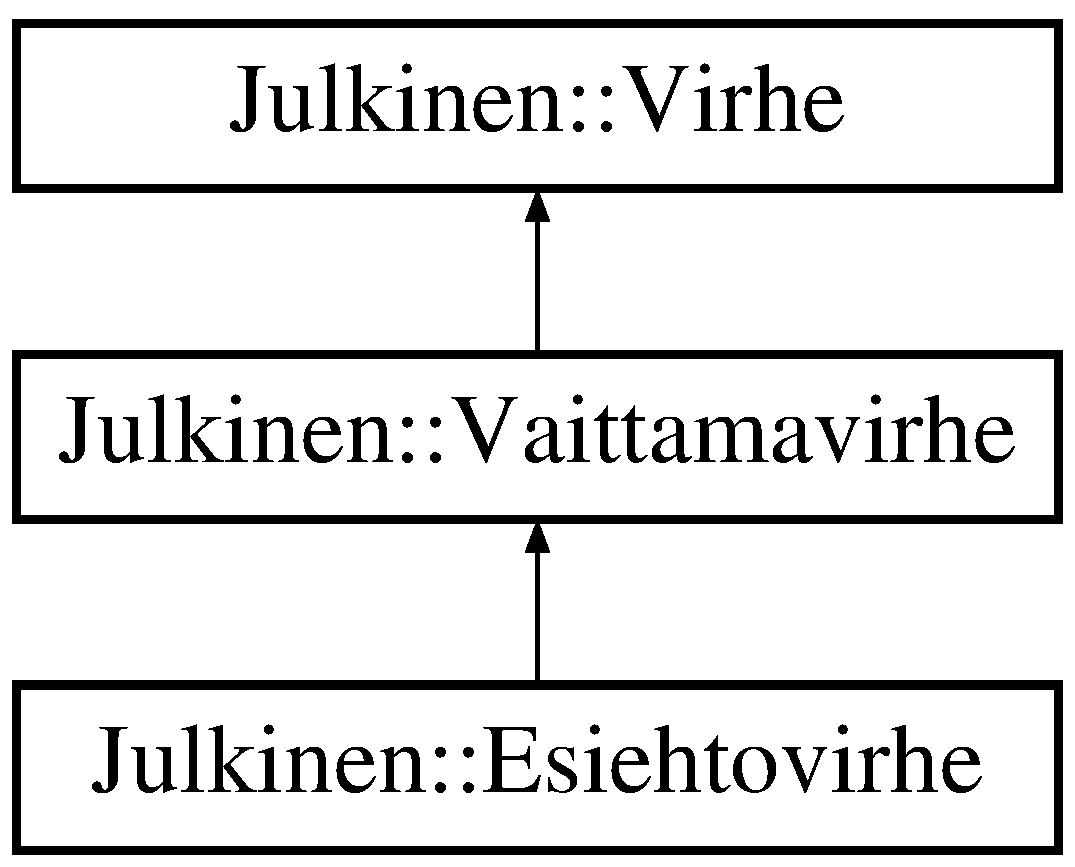
\includegraphics[height=3.000000cm]{class_julkinen_1_1_esiehtovirhe}
\end{center}
\end{figure}
\subsection*{Public Member Functions}
\begin{DoxyCompactItemize}
\item 
\hyperlink{class_julkinen_1_1_esiehtovirhe_a9be27b8ea22c7ff666af78925e164e39}{Esiehtovirhe} (char const $\ast$lauseke, char const $\ast$\hyperlink{class_julkinen_1_1_vaittamavirhe_a8624cd880b8466188ef6de480431dffb}{tiedosto}, unsigned int \hyperlink{class_julkinen_1_1_vaittamavirhe_abc571141231b3fa789ae41d2d80642ef}{rivi}, char const $\ast$\hyperlink{class_julkinen_1_1_vaittamavirhe_afd5de6b5639336288d28fd077c84a20c}{funktio})  throw ()
\begin{DoxyCompactList}\small\item\em \hyperlink{class_julkinen_1_1_esiehtovirhe}{Esiehtovirhe} rakentaja. \end{DoxyCompactList}\item 
\hypertarget{class_julkinen_1_1_esiehtovirhe_af5b91194864702d56a2679af08cc7384}{}virtual \hyperlink{class_julkinen_1_1_esiehtovirhe_af5b91194864702d56a2679af08cc7384}{$\sim$\+Esiehtovirhe} ()  throw ()\label{class_julkinen_1_1_esiehtovirhe_af5b91194864702d56a2679af08cc7384}

\begin{DoxyCompactList}\small\item\em Purkaja. \end{DoxyCompactList}\item 
virtual std\+::basic\+\_\+ostream$<$ char $>$ \& \hyperlink{class_julkinen_1_1_esiehtovirhe_a333610e4679e467075bd02c37b9e49bf}{tulosta} (std\+::basic\+\_\+ostream$<$ char $>$ \&tuloste) const 
\begin{DoxyCompactList}\small\item\em Tulostus virran luonti metodi. \end{DoxyCompactList}\end{DoxyCompactItemize}
\subsection*{Additional Inherited Members}


\subsection{Detailed Description}
Invariantti assertin lähettämän virhe. 

\subsection{Constructor \& Destructor Documentation}
\hypertarget{class_julkinen_1_1_esiehtovirhe_a9be27b8ea22c7ff666af78925e164e39}{}\index{Julkinen\+::\+Esiehtovirhe@{Julkinen\+::\+Esiehtovirhe}!Esiehtovirhe@{Esiehtovirhe}}
\index{Esiehtovirhe@{Esiehtovirhe}!Julkinen\+::\+Esiehtovirhe@{Julkinen\+::\+Esiehtovirhe}}
\subsubsection[{Esiehtovirhe(char const $\ast$lauseke, char const $\ast$tiedosto, unsigned int rivi, char const $\ast$funktio)}]{\setlength{\rightskip}{0pt plus 5cm}Esiehtovirhe\+::\+Esiehtovirhe (
\begin{DoxyParamCaption}
\item[{char const $\ast$}]{lauseke, }
\item[{char const $\ast$}]{tiedosto, }
\item[{unsigned int}]{rivi, }
\item[{char const $\ast$}]{funktio}
\end{DoxyParamCaption}
) throw  ) }\label{class_julkinen_1_1_esiehtovirhe_a9be27b8ea22c7ff666af78925e164e39}


\hyperlink{class_julkinen_1_1_esiehtovirhe}{Esiehtovirhe} rakentaja. 


\begin{DoxyParams}{Parameters}
{\em lauseke} & Merkkijono. \\
\hline
{\em tiedosto} & Merkkijono. \\
\hline
{\em rivi} & Rivinumero. \\
\hline
{\em funktio} & Merkkijono. \\
\hline
\end{DoxyParams}


\subsection{Member Function Documentation}
\hypertarget{class_julkinen_1_1_esiehtovirhe_a333610e4679e467075bd02c37b9e49bf}{}\index{Julkinen\+::\+Esiehtovirhe@{Julkinen\+::\+Esiehtovirhe}!tulosta@{tulosta}}
\index{tulosta@{tulosta}!Julkinen\+::\+Esiehtovirhe@{Julkinen\+::\+Esiehtovirhe}}
\subsubsection[{tulosta(std\+::basic\+\_\+ostream$<$ char $>$ \&tuloste) const }]{\setlength{\rightskip}{0pt plus 5cm}basic\+\_\+ostream$<$ char $>$ \& Esiehtovirhe\+::tulosta (
\begin{DoxyParamCaption}
\item[{std\+::basic\+\_\+ostream$<$ char $>$ \&}]{tuloste}
\end{DoxyParamCaption}
) const\hspace{0.3cm}{\ttfamily [virtual]}}\label{class_julkinen_1_1_esiehtovirhe_a333610e4679e467075bd02c37b9e49bf}


Tulostus virran luonti metodi. 


\begin{DoxyParams}{Parameters}
{\em tuloste} & Perus tulostevirta. \\
\hline
\end{DoxyParams}
\begin{DoxyReturn}{Returns}
Palauttaa perus tulostevirran. 
\end{DoxyReturn}


Reimplemented from \hyperlink{class_julkinen_1_1_virhe_a36a2644943038f9760b5d76a1960b00d}{Julkinen\+::\+Virhe}.



The documentation for this class was generated from the following files\+:\begin{DoxyCompactItemize}
\item 
valmiiden\+\_\+toteutus/include/\hyperlink{esiehtovirhe_8hh}{esiehtovirhe.\+hh}\item 
valmiiden\+\_\+toteutus/\hyperlink{esiehtovirhe_8cc}{esiehtovirhe.\+cc}\end{DoxyCompactItemize}

\hypertarget{class_esine}{}\section{Esine Class Reference}
\label{class_esine}\index{Esine@{Esine}}


Labyrintti-\/pelin esineen tietoluokka.  




{\ttfamily \#include $<$Esine.\+hpp$>$}

\subsection*{Public Member Functions}
\begin{DoxyCompactItemize}
\item 
\hyperlink{class_esine_ad3befbd3eb2ffa0993c2034e854cfadb}{Esine} ()
\begin{DoxyCompactList}\small\item\em Esineen tyhjä rakentaja. \end{DoxyCompactList}\item 
\hyperlink{class_esine_a62fb40b64b3f2773942dc609d415b521}{Esine} (char merkki, std\+::string pelaaja)
\begin{DoxyCompactList}\small\item\em Esineen kuormitettu rakentaja. \end{DoxyCompactList}\item 
\hyperlink{class_esine_a5d681e9b20aed1f63eda76c181c99ac4}{$\sim$\+Esine} ()
\begin{DoxyCompactList}\small\item\em Purkaja. \end{DoxyCompactList}\end{DoxyCompactItemize}
\subsection*{Public Attributes}
\begin{DoxyCompactItemize}
\item 
\hypertarget{class_esine_a8fc000d89cd0926b864c6242b9b51192}{}char {\bfseries merkki}\label{class_esine_a8fc000d89cd0926b864c6242b9b51192}

\item 
\hypertarget{class_esine_acbd8cbb1e704ecb09c75004ae29ad45f}{}std\+::string {\bfseries pelaaja}\label{class_esine_acbd8cbb1e704ecb09c75004ae29ad45f}

\end{DoxyCompactItemize}


\subsection{Detailed Description}
Labyrintti-\/pelin esineen tietoluokka. 

\subsection{Constructor \& Destructor Documentation}
\hypertarget{class_esine_ad3befbd3eb2ffa0993c2034e854cfadb}{}\index{Esine@{Esine}!Esine@{Esine}}
\index{Esine@{Esine}!Esine@{Esine}}
\subsubsection[{Esine()}]{\setlength{\rightskip}{0pt plus 5cm}Esine\+::\+Esine (
\begin{DoxyParamCaption}
{}
\end{DoxyParamCaption}
)}\label{class_esine_ad3befbd3eb2ffa0993c2034e854cfadb}


Esineen tyhjä rakentaja. 

Alustaa muuttujat.

\begin{DoxyPostcond}{Postcondition}
Muuttujat on alustettu. 
\end{DoxyPostcond}
\hypertarget{class_esine_a62fb40b64b3f2773942dc609d415b521}{}\index{Esine@{Esine}!Esine@{Esine}}
\index{Esine@{Esine}!Esine@{Esine}}
\subsubsection[{Esine(char merkki, std\+::string pelaaja)}]{\setlength{\rightskip}{0pt plus 5cm}Esine\+::\+Esine (
\begin{DoxyParamCaption}
\item[{char}]{merkki, }
\item[{std\+::string}]{pelaaja}
\end{DoxyParamCaption}
)}\label{class_esine_a62fb40b64b3f2773942dc609d415b521}


Esineen kuormitettu rakentaja. 

Alustaa muuttujat annettuihin arvoihin. 
\begin{DoxyParams}[1]{Parameters}
\mbox{\tt in}  & {\em merkki} & {\ttfamily Esineen} merkki. \\
\hline
\mbox{\tt in}  & {\em pelaaja} & {\ttfamily Esineen} pelaajan nimi.\\
\hline
\end{DoxyParams}
\begin{DoxyPostcond}{Postcondition}
Muuttujat on alustettu. 
\end{DoxyPostcond}
\hypertarget{class_esine_a5d681e9b20aed1f63eda76c181c99ac4}{}\index{Esine@{Esine}!````~Esine@{$\sim$\+Esine}}
\index{````~Esine@{$\sim$\+Esine}!Esine@{Esine}}
\subsubsection[{$\sim$\+Esine()}]{\setlength{\rightskip}{0pt plus 5cm}Esine\+::$\sim$\+Esine (
\begin{DoxyParamCaption}
{}
\end{DoxyParamCaption}
)}\label{class_esine_a5d681e9b20aed1f63eda76c181c99ac4}


Purkaja. 

\begin{DoxyPostcond}{Postcondition}
No-\/throw takuu. 
\end{DoxyPostcond}


The documentation for this class was generated from the following files\+:\begin{DoxyCompactItemize}
\item 
\hyperlink{_esine_8hpp}{Esine.\+hpp}\item 
Esine.\+cpp\end{DoxyCompactItemize}

\hypertarget{class_julkinen_1_1_invarianttivirhe}{}\section{Julkinen\+:\+:Invarianttivirhe Class Reference}
\label{class_julkinen_1_1_invarianttivirhe}\index{Julkinen\+::\+Invarianttivirhe@{Julkinen\+::\+Invarianttivirhe}}


Invariantti assertin lähettämän virhe.  




{\ttfamily \#include $<$invarianttivirhe.\+hh$>$}

Inheritance diagram for Julkinen\+:\+:Invarianttivirhe\+:\begin{figure}[H]
\begin{center}
\leavevmode
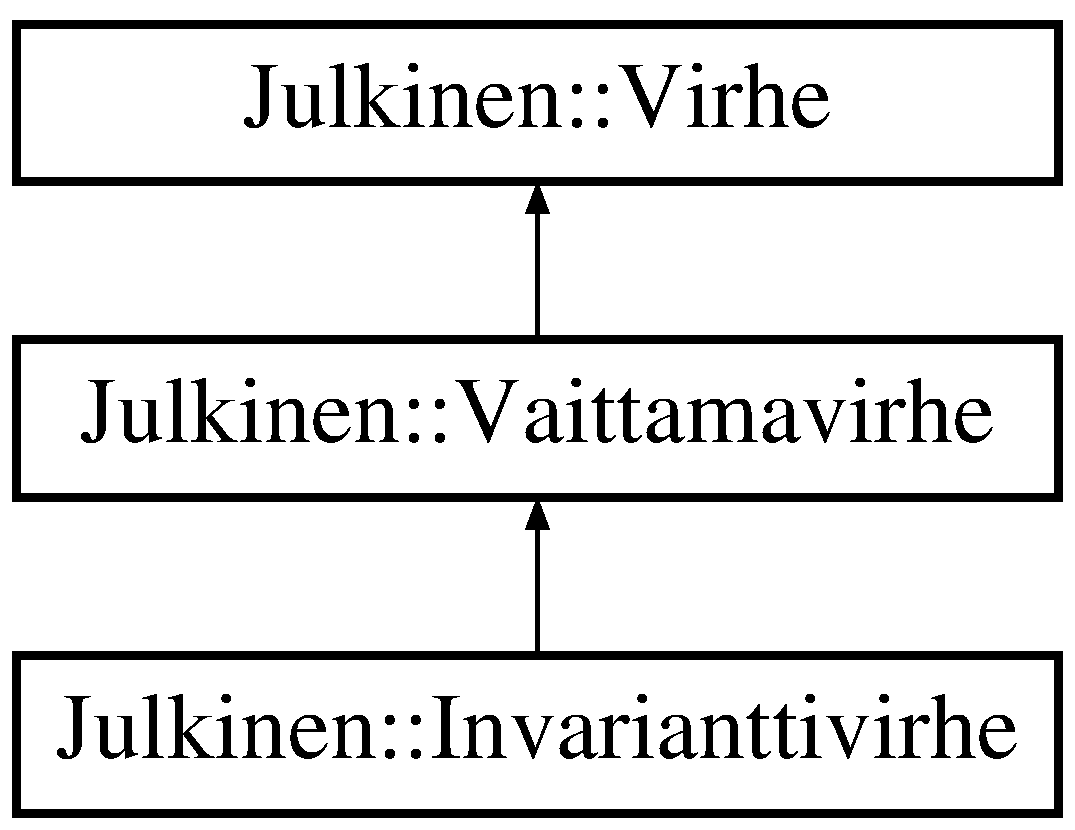
\includegraphics[height=3.000000cm]{class_julkinen_1_1_invarianttivirhe}
\end{center}
\end{figure}
\subsection*{Public Member Functions}
\begin{DoxyCompactItemize}
\item 
\hyperlink{class_julkinen_1_1_invarianttivirhe_a946670cc26aff5883b3dd4edb2e8e988}{Invarianttivirhe} (char const $\ast$lauseke, char const $\ast$\hyperlink{class_julkinen_1_1_vaittamavirhe_a8624cd880b8466188ef6de480431dffb}{tiedosto}, unsigned int \hyperlink{class_julkinen_1_1_vaittamavirhe_abc571141231b3fa789ae41d2d80642ef}{rivi}, char const $\ast$\hyperlink{class_julkinen_1_1_vaittamavirhe_afd5de6b5639336288d28fd077c84a20c}{funktio})  throw ()
\begin{DoxyCompactList}\small\item\em \hyperlink{class_julkinen_1_1_invarianttivirhe}{Invarianttivirhe} rakentaja. \end{DoxyCompactList}\item 
\hypertarget{class_julkinen_1_1_invarianttivirhe_a34c1aa9b2cbd4e58adfb3646d86eb7c0}{}\hyperlink{class_julkinen_1_1_invarianttivirhe_a34c1aa9b2cbd4e58adfb3646d86eb7c0}{$\sim$\+Invarianttivirhe} ()  throw ()\label{class_julkinen_1_1_invarianttivirhe_a34c1aa9b2cbd4e58adfb3646d86eb7c0}

\begin{DoxyCompactList}\small\item\em Purkaja. \end{DoxyCompactList}\item 
std\+::basic\+\_\+ostream$<$ char $>$ \& \hyperlink{class_julkinen_1_1_invarianttivirhe_ac0f90f4d0915c90c14d752a64da5196a}{tulosta} (std\+::basic\+\_\+ostream$<$ char $>$ \&tuloste) const 
\begin{DoxyCompactList}\small\item\em Tulostus virran luonti metodi. \end{DoxyCompactList}\end{DoxyCompactItemize}
\subsection*{Additional Inherited Members}


\subsection{Detailed Description}
Invariantti assertin lähettämän virhe. 

\subsection{Constructor \& Destructor Documentation}
\hypertarget{class_julkinen_1_1_invarianttivirhe_a946670cc26aff5883b3dd4edb2e8e988}{}\index{Julkinen\+::\+Invarianttivirhe@{Julkinen\+::\+Invarianttivirhe}!Invarianttivirhe@{Invarianttivirhe}}
\index{Invarianttivirhe@{Invarianttivirhe}!Julkinen\+::\+Invarianttivirhe@{Julkinen\+::\+Invarianttivirhe}}
\subsubsection[{Invarianttivirhe(char const $\ast$lauseke, char const $\ast$tiedosto, unsigned int rivi, char const $\ast$funktio)}]{\setlength{\rightskip}{0pt plus 5cm}Invarianttivirhe\+::\+Invarianttivirhe (
\begin{DoxyParamCaption}
\item[{char const $\ast$}]{lauseke, }
\item[{char const $\ast$}]{tiedosto, }
\item[{unsigned int}]{rivi, }
\item[{char const $\ast$}]{funktio}
\end{DoxyParamCaption}
) throw  ) }\label{class_julkinen_1_1_invarianttivirhe_a946670cc26aff5883b3dd4edb2e8e988}


\hyperlink{class_julkinen_1_1_invarianttivirhe}{Invarianttivirhe} rakentaja. 


\begin{DoxyParams}{Parameters}
{\em lauseke} & Merkkijono. \\
\hline
{\em tiedosto} & Merkkijono. \\
\hline
{\em rivi} & Rivinumero. \\
\hline
{\em funktio} & Merkkijono. \\
\hline
\end{DoxyParams}


\subsection{Member Function Documentation}
\hypertarget{class_julkinen_1_1_invarianttivirhe_ac0f90f4d0915c90c14d752a64da5196a}{}\index{Julkinen\+::\+Invarianttivirhe@{Julkinen\+::\+Invarianttivirhe}!tulosta@{tulosta}}
\index{tulosta@{tulosta}!Julkinen\+::\+Invarianttivirhe@{Julkinen\+::\+Invarianttivirhe}}
\subsubsection[{tulosta(std\+::basic\+\_\+ostream$<$ char $>$ \&tuloste) const }]{\setlength{\rightskip}{0pt plus 5cm}basic\+\_\+ostream$<$ char $>$ \& Invarianttivirhe\+::tulosta (
\begin{DoxyParamCaption}
\item[{std\+::basic\+\_\+ostream$<$ char $>$ \&}]{tuloste}
\end{DoxyParamCaption}
) const\hspace{0.3cm}{\ttfamily [virtual]}}\label{class_julkinen_1_1_invarianttivirhe_ac0f90f4d0915c90c14d752a64da5196a}


Tulostus virran luonti metodi. 


\begin{DoxyParams}{Parameters}
{\em tuloste} & Perus tulostevirta. \\
\hline
\end{DoxyParams}
\begin{DoxyReturn}{Returns}
Palauttaa perus tulostevirran. 
\end{DoxyReturn}


Reimplemented from \hyperlink{class_julkinen_1_1_virhe_a36a2644943038f9760b5d76a1960b00d}{Julkinen\+::\+Virhe}.



The documentation for this class was generated from the following files\+:\begin{DoxyCompactItemize}
\item 
valmiiden\+\_\+toteutus/include/\hyperlink{invarianttivirhe_8hh}{invarianttivirhe.\+hh}\item 
valmiiden\+\_\+toteutus/\hyperlink{invarianttivirhe_8cc}{invarianttivirhe.\+cc}\end{DoxyCompactItemize}

\hypertarget{class_julkinen_1_1_jalkiehtovirhe}{}\section{Julkinen\+:\+:Jalkiehtovirhe Class Reference}
\label{class_julkinen_1_1_jalkiehtovirhe}\index{Julkinen\+::\+Jalkiehtovirhe@{Julkinen\+::\+Jalkiehtovirhe}}


Jälkiehto assertin lähettämän virhe.  




{\ttfamily \#include $<$jalkiehtovirhe.\+hh$>$}

Inheritance diagram for Julkinen\+:\+:Jalkiehtovirhe\+:\begin{figure}[H]
\begin{center}
\leavevmode
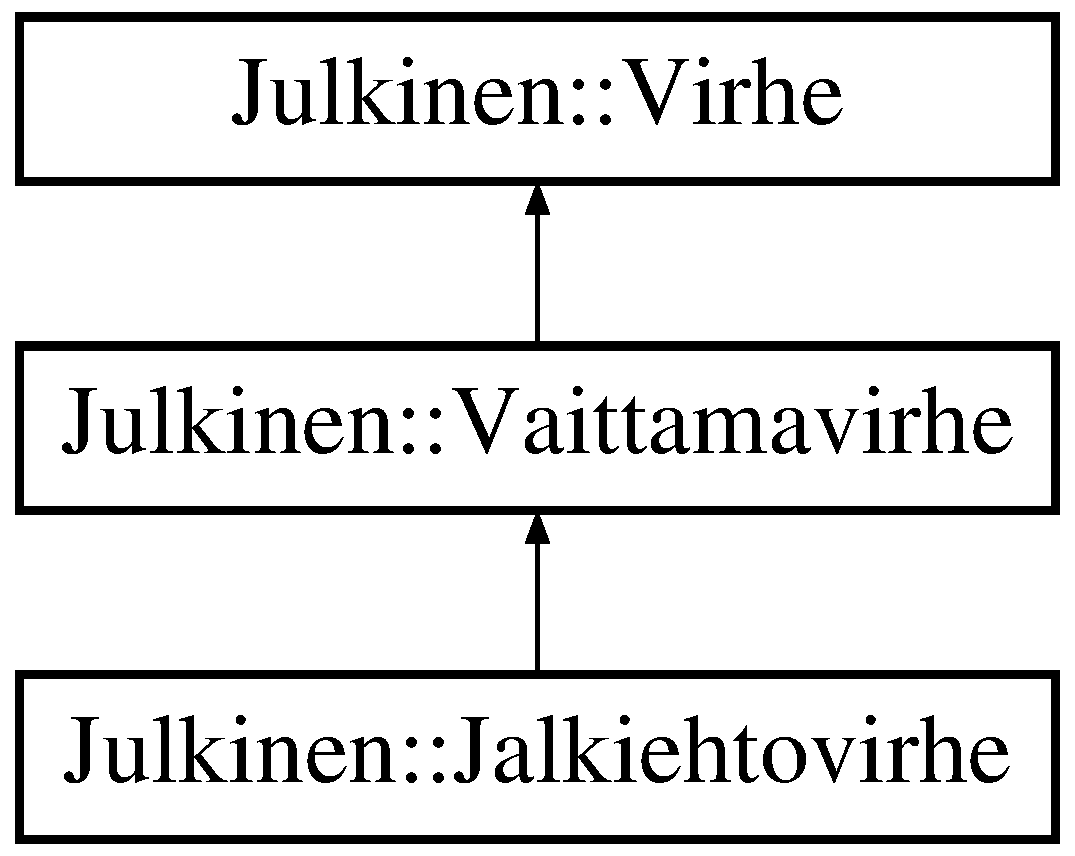
\includegraphics[height=3.000000cm]{class_julkinen_1_1_jalkiehtovirhe}
\end{center}
\end{figure}
\subsection*{Public Member Functions}
\begin{DoxyCompactItemize}
\item 
\hyperlink{class_julkinen_1_1_jalkiehtovirhe_a23d92ebad4c84c880bef9ddd48e21efb}{Jalkiehtovirhe} (char const $\ast$lauseke, char const $\ast$\hyperlink{class_julkinen_1_1_vaittamavirhe_a8624cd880b8466188ef6de480431dffb}{tiedosto}, unsigned int \hyperlink{class_julkinen_1_1_vaittamavirhe_abc571141231b3fa789ae41d2d80642ef}{rivi}, char const $\ast$\hyperlink{class_julkinen_1_1_vaittamavirhe_afd5de6b5639336288d28fd077c84a20c}{funktio})  throw ()
\begin{DoxyCompactList}\small\item\em \hyperlink{class_julkinen_1_1_jalkiehtovirhe}{Jalkiehtovirhe} rakentaja. \end{DoxyCompactList}\item 
\hypertarget{class_julkinen_1_1_jalkiehtovirhe_a2ac148c53e973b52e7f9bcc8b3c785d5}{}\hyperlink{class_julkinen_1_1_jalkiehtovirhe_a2ac148c53e973b52e7f9bcc8b3c785d5}{$\sim$\+Jalkiehtovirhe} ()  throw ()\label{class_julkinen_1_1_jalkiehtovirhe_a2ac148c53e973b52e7f9bcc8b3c785d5}

\begin{DoxyCompactList}\small\item\em Purkaja. \end{DoxyCompactList}\item 
std\+::basic\+\_\+ostream$<$ char $>$ \& \hyperlink{class_julkinen_1_1_jalkiehtovirhe_a5cbdae2671dfaa4700a9118048c7570e}{tulosta} (std\+::basic\+\_\+ostream$<$ char $>$ \&tuloste) const 
\begin{DoxyCompactList}\small\item\em Tulostus virran luonti metodi. \end{DoxyCompactList}\end{DoxyCompactItemize}
\subsection*{Additional Inherited Members}


\subsection{Detailed Description}
Jälkiehto assertin lähettämän virhe. 

\subsection{Constructor \& Destructor Documentation}
\hypertarget{class_julkinen_1_1_jalkiehtovirhe_a23d92ebad4c84c880bef9ddd48e21efb}{}\index{Julkinen\+::\+Jalkiehtovirhe@{Julkinen\+::\+Jalkiehtovirhe}!Jalkiehtovirhe@{Jalkiehtovirhe}}
\index{Jalkiehtovirhe@{Jalkiehtovirhe}!Julkinen\+::\+Jalkiehtovirhe@{Julkinen\+::\+Jalkiehtovirhe}}
\subsubsection[{Jalkiehtovirhe(char const $\ast$lauseke, char const $\ast$tiedosto, unsigned int rivi, char const $\ast$funktio)}]{\setlength{\rightskip}{0pt plus 5cm}Jalkiehtovirhe\+::\+Jalkiehtovirhe (
\begin{DoxyParamCaption}
\item[{char const $\ast$}]{lauseke, }
\item[{char const $\ast$}]{tiedosto, }
\item[{unsigned int}]{rivi, }
\item[{char const $\ast$}]{funktio}
\end{DoxyParamCaption}
) throw  ) }\label{class_julkinen_1_1_jalkiehtovirhe_a23d92ebad4c84c880bef9ddd48e21efb}


\hyperlink{class_julkinen_1_1_jalkiehtovirhe}{Jalkiehtovirhe} rakentaja. 


\begin{DoxyParams}{Parameters}
{\em lauseke} & Merkkijono. \\
\hline
{\em tiedosto} & Merkkijono. \\
\hline
{\em rivi} & Rivinumero. \\
\hline
{\em funktio} & Merkkijono. \\
\hline
\end{DoxyParams}


\subsection{Member Function Documentation}
\hypertarget{class_julkinen_1_1_jalkiehtovirhe_a5cbdae2671dfaa4700a9118048c7570e}{}\index{Julkinen\+::\+Jalkiehtovirhe@{Julkinen\+::\+Jalkiehtovirhe}!tulosta@{tulosta}}
\index{tulosta@{tulosta}!Julkinen\+::\+Jalkiehtovirhe@{Julkinen\+::\+Jalkiehtovirhe}}
\subsubsection[{tulosta(std\+::basic\+\_\+ostream$<$ char $>$ \&tuloste) const }]{\setlength{\rightskip}{0pt plus 5cm}basic\+\_\+ostream$<$ char $>$ \& Jalkiehtovirhe\+::tulosta (
\begin{DoxyParamCaption}
\item[{std\+::basic\+\_\+ostream$<$ char $>$ \&}]{tuloste}
\end{DoxyParamCaption}
) const\hspace{0.3cm}{\ttfamily [virtual]}}\label{class_julkinen_1_1_jalkiehtovirhe_a5cbdae2671dfaa4700a9118048c7570e}


Tulostus virran luonti metodi. 


\begin{DoxyParams}{Parameters}
{\em tuloste} & Perus tulostevirta. \\
\hline
\end{DoxyParams}
\begin{DoxyReturn}{Returns}
Palauttaa perus tulostevirran. 
\end{DoxyReturn}


Reimplemented from \hyperlink{class_julkinen_1_1_virhe_a36a2644943038f9760b5d76a1960b00d}{Julkinen\+::\+Virhe}.



The documentation for this class was generated from the following files\+:\begin{DoxyCompactItemize}
\item 
valmiiden\+\_\+toteutus/include/\hyperlink{jalkiehtovirhe_8hh}{jalkiehtovirhe.\+hh}\item 
valmiiden\+\_\+toteutus/\hyperlink{jalkiehtovirhe_8cc}{jalkiehtovirhe.\+cc}\end{DoxyCompactItemize}

\hypertarget{class_komentotulkki}{}\section{Komentotulkki Class Reference}
\label{class_komentotulkki}\index{Komentotulkki@{Komentotulkki}}


Komentotulkin toteuttava luokka.  




{\ttfamily \#include $<$komentotulkki.\+hh$>$}

\subsection*{Public Member Functions}
\begin{DoxyCompactItemize}
\item 
void \hyperlink{class_komentotulkki_a3c9372e77cf9e4dbd741572f6445a106}{kaynnista\+Komentotulkki} (std\+::shared\+\_\+ptr$<$ \hyperlink{class_julkinen_1_1_pelirajapinta}{Julkinen\+::\+Pelirajapinta} $>$ peli)
\begin{DoxyCompactList}\small\item\em Metodi komentotulkin käynnistämiseen. \end{DoxyCompactList}\end{DoxyCompactItemize}
\subsection*{Static Public Member Functions}
\begin{DoxyCompactItemize}
\item 
static std\+::shared\+\_\+ptr$<$ \hyperlink{class_komentotulkki}{Komentotulkki} $>$ \hyperlink{class_komentotulkki_ad7a004ae7aac2fe0b28a21d84c9a0fb9}{uusi\+Komentotulkki} (std\+::shared\+\_\+ptr$<$ \hyperlink{class_naytto}{Naytto} $>$ naytto)
\begin{DoxyCompactList}\small\item\em Luo {\ttfamily \hyperlink{class_komentotulkki}{Komentotulkki}} olion ja palauttaa osoittimen siihen. \end{DoxyCompactList}\item 
static void \hyperlink{class_komentotulkki_ae87386f32d344bdb497a68da55a9a718}{aseta\+Raakile\+Tilaan} ()
\begin{DoxyCompactList}\small\item\em Asettaa komentotulkin raakile tilaan. \end{DoxyCompactList}\item 
\hypertarget{class_komentotulkki_a96d3141f3af61972998c5c6deb64c2ac}{}static bool \hyperlink{class_komentotulkki_a96d3141f3af61972998c5c6deb64c2ac}{onko\+Raakile\+Tilassa} ()\label{class_komentotulkki_a96d3141f3af61972998c5c6deb64c2ac}

\begin{DoxyCompactList}\small\item\em Kysyy, onko komentotulkki raakiletilassa. \end{DoxyCompactList}\end{DoxyCompactItemize}


\subsection{Detailed Description}
Komentotulkin toteuttava luokka. 

Jos kääntäjä on G\+N\+U\+G pohjainen esim. gcc tai tutg++ käytetään tr1/memory kirjastoa. 

\subsection{Member Function Documentation}
\hypertarget{class_komentotulkki_ae87386f32d344bdb497a68da55a9a718}{}\index{Komentotulkki@{Komentotulkki}!aseta\+Raakile\+Tilaan@{aseta\+Raakile\+Tilaan}}
\index{aseta\+Raakile\+Tilaan@{aseta\+Raakile\+Tilaan}!Komentotulkki@{Komentotulkki}}
\subsubsection[{aseta\+Raakile\+Tilaan()}]{\setlength{\rightskip}{0pt plus 5cm}void Komentotulkki\+::aseta\+Raakile\+Tilaan (
\begin{DoxyParamCaption}
{}
\end{DoxyParamCaption}
)\hspace{0.3cm}{\ttfamily [static]}}\label{class_komentotulkki_ae87386f32d344bdb497a68da55a9a718}


Asettaa komentotulkin raakile tilaan. 

\begin{DoxyPostcond}{Postcondition}
\hyperlink{class_komentotulkki}{Komentotulkki} on raakile tilassa. 
\end{DoxyPostcond}
\hypertarget{class_komentotulkki_a3c9372e77cf9e4dbd741572f6445a106}{}\index{Komentotulkki@{Komentotulkki}!kaynnista\+Komentotulkki@{kaynnista\+Komentotulkki}}
\index{kaynnista\+Komentotulkki@{kaynnista\+Komentotulkki}!Komentotulkki@{Komentotulkki}}
\subsubsection[{kaynnista\+Komentotulkki(std\+::shared\+\_\+ptr$<$ Julkinen\+::\+Pelirajapinta $>$ peli)}]{\setlength{\rightskip}{0pt plus 5cm}void Komentotulkki\+::kaynnista\+Komentotulkki (
\begin{DoxyParamCaption}
\item[{std\+::shared\+\_\+ptr$<$ {\bf Julkinen\+::\+Pelirajapinta} $>$}]{peli}
\end{DoxyParamCaption}
)}\label{class_komentotulkki_a3c9372e77cf9e4dbd741572f6445a106}


Metodi komentotulkin käynnistämiseen. 

\begin{DoxyPrecond}{Precondition}
\hyperlink{class_peli}{Peli} on pelitilassa. 
\end{DoxyPrecond}
\begin{DoxyPostcond}{Postcondition}
\hyperlink{class_komentotulkki}{Komentotulkki} on käynnistetty.
\end{DoxyPostcond}

\begin{DoxyParams}{Parameters}
{\em peli} & Osoitin peliin. \\
\hline
\end{DoxyParams}
\hypertarget{class_komentotulkki_ad7a004ae7aac2fe0b28a21d84c9a0fb9}{}\index{Komentotulkki@{Komentotulkki}!uusi\+Komentotulkki@{uusi\+Komentotulkki}}
\index{uusi\+Komentotulkki@{uusi\+Komentotulkki}!Komentotulkki@{Komentotulkki}}
\subsubsection[{uusi\+Komentotulkki(std\+::shared\+\_\+ptr$<$ Naytto $>$ naytto)}]{\setlength{\rightskip}{0pt plus 5cm}std\+::shared\+\_\+ptr$<$ {\bf Komentotulkki} $>$ Komentotulkki\+::uusi\+Komentotulkki (
\begin{DoxyParamCaption}
\item[{std\+::shared\+\_\+ptr$<$ {\bf Naytto} $>$}]{naytto}
\end{DoxyParamCaption}
)\hspace{0.3cm}{\ttfamily [static]}}\label{class_komentotulkki_ad7a004ae7aac2fe0b28a21d84c9a0fb9}


Luo {\ttfamily \hyperlink{class_komentotulkki}{Komentotulkki}} olion ja palauttaa osoittimen siihen. 

\begin{DoxyPostcond}{Postcondition}
Palauttanut jaetunosoittiminen \hyperlink{class_komentotulkki}{Komentotulkki} -\/osoittimeen.
\end{DoxyPostcond}
\begin{DoxyReturn}{Returns}
Palauttaa osoittimen komenttotulkki olioon. 
\end{DoxyReturn}


The documentation for this class was generated from the following files\+:\begin{DoxyCompactItemize}
\item 
valmiiden\+\_\+toteutus/include/\hyperlink{komentotulkki_8hh}{komentotulkki.\+hh}\item 
valmiiden\+\_\+toteutus/\hyperlink{komentotulkki_8cc}{komentotulkki.\+cc}\end{DoxyCompactItemize}

\hypertarget{class_julkinen_1_1_komentovirhe}{}\section{Julkinen\+:\+:Komentovirhe Class Reference}
\label{class_julkinen_1_1_komentovirhe}\index{Julkinen\+::\+Komentovirhe@{Julkinen\+::\+Komentovirhe}}


Käyttäjän antamaa pelikomentoa ei saatu suoritettua.  




{\ttfamily \#include $<$komentovirhe.\+hh$>$}

Inheritance diagram for Julkinen\+:\+:Komentovirhe\+:\begin{figure}[H]
\begin{center}
\leavevmode
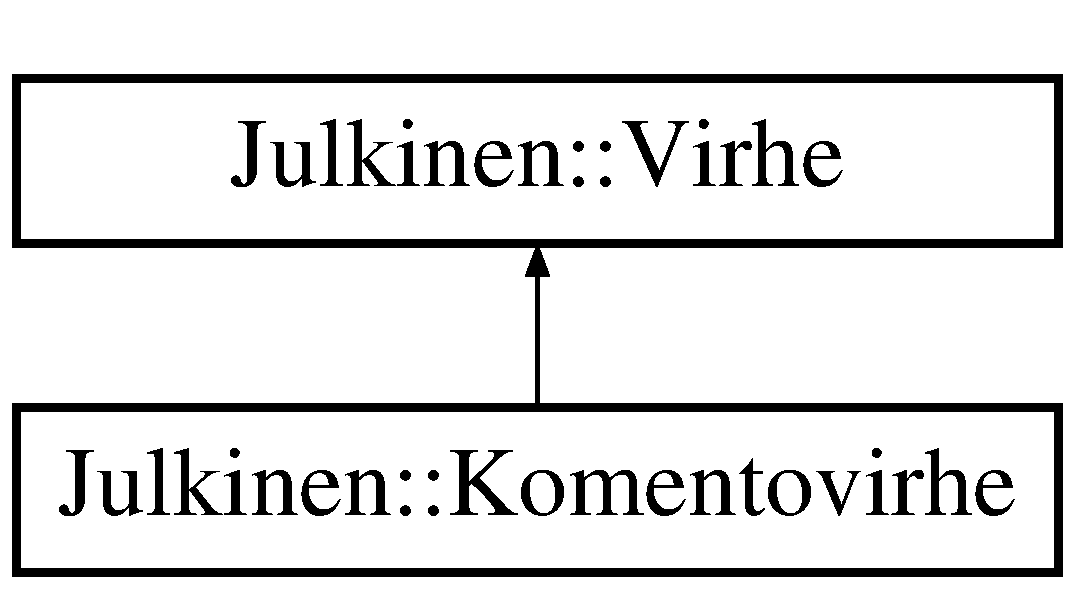
\includegraphics[height=2.000000cm]{class_julkinen_1_1_komentovirhe}
\end{center}
\end{figure}
\subsection*{Public Types}
\begin{DoxyCompactItemize}
\item 
enum \hyperlink{class_julkinen_1_1_komentovirhe_ad45b4895d16e53f115875f2e2a1518e3}{Virhekoodi} \{ \\*
\hyperlink{class_julkinen_1_1_komentovirhe_ad45b4895d16e53f115875f2e2a1518e3ad138f8f3c9591bd14fe68ac15a9fa9c5}{V\+I\+R\+H\+E\+\_\+\+O\+L\+E\+M\+A\+T\+O\+N\+\_\+\+P\+A\+I\+K\+K\+A}, 
\hyperlink{class_julkinen_1_1_komentovirhe_ad45b4895d16e53f115875f2e2a1518e3ab36ab3ed54b561768d5815d4dbef8cd2}{V\+I\+R\+H\+E\+\_\+\+V\+I\+R\+H\+E\+E\+L\+L\+I\+N\+E\+N\+\_\+\+R\+O\+T\+A\+A\+T\+I\+O}, 
{\bfseries V\+I\+R\+H\+E\+\_\+\+T\+U\+N\+N\+I\+S\+T\+A\+M\+A\+T\+O\+N\+\_\+\+P\+A\+R\+A\+M\+E\+T\+R\+I}, 
{\bfseries V\+I\+R\+H\+E\+\_\+\+T\+U\+N\+N\+I\+S\+T\+A\+M\+A\+T\+O\+N\+\_\+\+K\+O\+M\+E\+N\+T\+O}, 
\\*
{\bfseries V\+I\+R\+H\+E\+\_\+\+L\+I\+I\+K\+A\+A\+\_\+\+P\+A\+R\+A\+M\+E\+T\+R\+E\+J\+A}, 
\hyperlink{class_julkinen_1_1_komentovirhe_ad45b4895d16e53f115875f2e2a1518e3a54f39d45fd85a02c18678c416337b4d8}{V\+I\+R\+H\+E\+\_\+\+T\+U\+N\+N\+I\+S\+T\+A\+M\+A\+T\+O\+N}
 \}\begin{DoxyCompactList}\small\item\em Tunnisteet esimääritellyille virhetilanteille käyttäjän antamissa komennoissa. \end{DoxyCompactList}
\end{DoxyCompactItemize}
\subsection*{Public Member Functions}
\begin{DoxyCompactItemize}
\item 
\hyperlink{class_julkinen_1_1_komentovirhe_a1247b5f9cf1f6d4aa59baa8384e0112e}{Komentovirhe} (std\+::string const \&virheviesti)
\begin{DoxyCompactList}\small\item\em Tunnistamaton virhetilanne kopioidulla viestillä. \end{DoxyCompactList}\item 
\hyperlink{class_julkinen_1_1_komentovirhe_ab1ef7899e248fb500629cce56633c556}{Komentovirhe} (\hyperlink{class_julkinen_1_1_komentovirhe_ad45b4895d16e53f115875f2e2a1518e3}{Virhekoodi} virhekoodi)
\begin{DoxyCompactList}\small\item\em Esimääritelty virhetilanne. \end{DoxyCompactList}\item 
\hyperlink{class_julkinen_1_1_komentovirhe_a821c0e04a608cb5d8a137df0c7a4327c}{Komentovirhe} (\hyperlink{class_julkinen_1_1_komentovirhe}{Komentovirhe} const \&toinen)
\begin{DoxyCompactList}\small\item\em Kopiorakentaja. \end{DoxyCompactList}\item 
\hyperlink{class_julkinen_1_1_komentovirhe}{Komentovirhe} \& \hyperlink{class_julkinen_1_1_komentovirhe_af734e3e8cf75a93652020efb15420def}{operator=} (\hyperlink{class_julkinen_1_1_komentovirhe}{Komentovirhe} const \&toinen)
\begin{DoxyCompactList}\small\item\em Sijoitusoperaattori. \end{DoxyCompactList}\item 
\hypertarget{class_julkinen_1_1_komentovirhe_a1b92df0f5dce8cec701f7f99801a5b1c}{}\hyperlink{class_julkinen_1_1_komentovirhe_ad45b4895d16e53f115875f2e2a1518e3}{Virhekoodi} \hyperlink{class_julkinen_1_1_komentovirhe_a1b92df0f5dce8cec701f7f99801a5b1c}{virhe} () const \label{class_julkinen_1_1_komentovirhe_a1b92df0f5dce8cec701f7f99801a5b1c}

\begin{DoxyCompactList}\small\item\em Sattuneen virhetilanteen virhekoodi. \end{DoxyCompactList}\item 
\hypertarget{class_julkinen_1_1_komentovirhe_a51d6d273b79074b6c8ea8d0b1ef2fe65}{}std\+::basic\+\_\+ostream$<$ char $>$ \& \hyperlink{class_julkinen_1_1_komentovirhe_a51d6d273b79074b6c8ea8d0b1ef2fe65}{tulosta} (std\+::basic\+\_\+ostream$<$ char $>$ \&tuloste) const \label{class_julkinen_1_1_komentovirhe_a51d6d273b79074b6c8ea8d0b1ef2fe65}

\begin{DoxyCompactList}\small\item\em Tulosta \char`\"{}\+V\+I\+R\+H\+E\+: \char`\"{} ja virhekoodiin liittyvä viesti. \end{DoxyCompactList}\end{DoxyCompactItemize}
\subsection*{Additional Inherited Members}


\subsection{Detailed Description}
Käyttäjän antamaa pelikomentoa ei saatu suoritettua. 

Mikäli käyttäjän ohjelmalle vuorovaikutteisesti antama komento on jotenkin virheellinen, heitetään tätä tyyppiä oleva poikkeus. Olio alustetaan jollakin esimääritellyistä virhekoodeista tai pelkällä virheviestillä. Virhekoodilla alustettaessa virheen viestiksi tulee sopiva selkokielinen viesti ja virheviestillä alustettaessa koodiksi tulee V\+I\+R\+H\+E\+\_\+\+T\+U\+N\+N\+I\+S\+T\+A\+M\+A\+T\+O\+N. Virheviestillä alustamista tulee käyttää vain sellaisille virhetilanteille, joille ei ole esimääriteltyä koodia. 

\subsection{Member Enumeration Documentation}
\hypertarget{class_julkinen_1_1_komentovirhe_ad45b4895d16e53f115875f2e2a1518e3}{}\index{Julkinen\+::\+Komentovirhe@{Julkinen\+::\+Komentovirhe}!Virhekoodi@{Virhekoodi}}
\index{Virhekoodi@{Virhekoodi}!Julkinen\+::\+Komentovirhe@{Julkinen\+::\+Komentovirhe}}
\subsubsection[{Virhekoodi}]{\setlength{\rightskip}{0pt plus 5cm}enum {\bf Julkinen\+::\+Komentovirhe\+::\+Virhekoodi}}\label{class_julkinen_1_1_komentovirhe_ad45b4895d16e53f115875f2e2a1518e3}


Tunnisteet esimääritellyille virhetilanteille käyttäjän antamissa komennoissa. 

! \begin{Desc}
\item[Enumerator]\par
\begin{description}
\index{V\+I\+R\+H\+E\+\_\+\+O\+L\+E\+M\+A\+T\+O\+N\+\_\+\+P\+A\+I\+K\+K\+A@{V\+I\+R\+H\+E\+\_\+\+O\+L\+E\+M\+A\+T\+O\+N\+\_\+\+P\+A\+I\+K\+K\+A}!Julkinen\+::\+Komentovirhe@{Julkinen\+::\+Komentovirhe}}\index{Julkinen\+::\+Komentovirhe@{Julkinen\+::\+Komentovirhe}!V\+I\+R\+H\+E\+\_\+\+O\+L\+E\+M\+A\+T\+O\+N\+\_\+\+P\+A\+I\+K\+K\+A@{V\+I\+R\+H\+E\+\_\+\+O\+L\+E\+M\+A\+T\+O\+N\+\_\+\+P\+A\+I\+K\+K\+A}}\item[{\em 
\hypertarget{class_julkinen_1_1_komentovirhe_ad45b4895d16e53f115875f2e2a1518e3ad138f8f3c9591bd14fe68ac15a9fa9c5}{}V\+I\+R\+H\+E\+\_\+\+O\+L\+E\+M\+A\+T\+O\+N\+\_\+\+P\+A\+I\+K\+K\+A\label{class_julkinen_1_1_komentovirhe_ad45b4895d16e53f115875f2e2a1518e3ad138f8f3c9591bd14fe68ac15a9fa9c5}
}]Annettua paikkaa ei ole kartalla. \index{V\+I\+R\+H\+E\+\_\+\+V\+I\+R\+H\+E\+E\+L\+L\+I\+N\+E\+N\+\_\+\+R\+O\+T\+A\+A\+T\+I\+O@{V\+I\+R\+H\+E\+\_\+\+V\+I\+R\+H\+E\+E\+L\+L\+I\+N\+E\+N\+\_\+\+R\+O\+T\+A\+A\+T\+I\+O}!Julkinen\+::\+Komentovirhe@{Julkinen\+::\+Komentovirhe}}\index{Julkinen\+::\+Komentovirhe@{Julkinen\+::\+Komentovirhe}!V\+I\+R\+H\+E\+\_\+\+V\+I\+R\+H\+E\+E\+L\+L\+I\+N\+E\+N\+\_\+\+R\+O\+T\+A\+A\+T\+I\+O@{V\+I\+R\+H\+E\+\_\+\+V\+I\+R\+H\+E\+E\+L\+L\+I\+N\+E\+N\+\_\+\+R\+O\+T\+A\+A\+T\+I\+O}}\item[{\em 
\hypertarget{class_julkinen_1_1_komentovirhe_ad45b4895d16e53f115875f2e2a1518e3ab36ab3ed54b561768d5815d4dbef8cd2}{}V\+I\+R\+H\+E\+\_\+\+V\+I\+R\+H\+E\+E\+L\+L\+I\+N\+E\+N\+\_\+\+R\+O\+T\+A\+A\+T\+I\+O\label{class_julkinen_1_1_komentovirhe_ad45b4895d16e53f115875f2e2a1518e3ab36ab3ed54b561768d5815d4dbef8cd2}
}]Annettu rotaatio on virheellinen. \index{V\+I\+R\+H\+E\+\_\+\+T\+U\+N\+N\+I\+S\+T\+A\+M\+A\+T\+O\+N@{V\+I\+R\+H\+E\+\_\+\+T\+U\+N\+N\+I\+S\+T\+A\+M\+A\+T\+O\+N}!Julkinen\+::\+Komentovirhe@{Julkinen\+::\+Komentovirhe}}\index{Julkinen\+::\+Komentovirhe@{Julkinen\+::\+Komentovirhe}!V\+I\+R\+H\+E\+\_\+\+T\+U\+N\+N\+I\+S\+T\+A\+M\+A\+T\+O\+N@{V\+I\+R\+H\+E\+\_\+\+T\+U\+N\+N\+I\+S\+T\+A\+M\+A\+T\+O\+N}}\item[{\em 
\hypertarget{class_julkinen_1_1_komentovirhe_ad45b4895d16e53f115875f2e2a1518e3a54f39d45fd85a02c18678c416337b4d8}{}V\+I\+R\+H\+E\+\_\+\+T\+U\+N\+N\+I\+S\+T\+A\+M\+A\+T\+O\+N\label{class_julkinen_1_1_komentovirhe_ad45b4895d16e53f115875f2e2a1518e3a54f39d45fd85a02c18678c416337b4d8}
}]Tunnistamaton virhe. \end{description}
\end{Desc}


\subsection{Constructor \& Destructor Documentation}
\hypertarget{class_julkinen_1_1_komentovirhe_a1247b5f9cf1f6d4aa59baa8384e0112e}{}\index{Julkinen\+::\+Komentovirhe@{Julkinen\+::\+Komentovirhe}!Komentovirhe@{Komentovirhe}}
\index{Komentovirhe@{Komentovirhe}!Julkinen\+::\+Komentovirhe@{Julkinen\+::\+Komentovirhe}}
\subsubsection[{Komentovirhe(std\+::string const \&virheviesti)}]{\setlength{\rightskip}{0pt plus 5cm}Komentovirhe\+::\+Komentovirhe (
\begin{DoxyParamCaption}
\item[{std\+::string const \&}]{virheviesti}
\end{DoxyParamCaption}
)\hspace{0.3cm}{\ttfamily [explicit]}}\label{class_julkinen_1_1_komentovirhe_a1247b5f9cf1f6d4aa59baa8384e0112e}


Tunnistamaton virhetilanne kopioidulla viestillä. 

Käytä tätä vain, jos kyseessä ei ole mikään esimääritellyistä virheistä.

\begin{DoxyPostcond}{Postcondition}
Perustakuu poikkeuksen sattuessa. 
\end{DoxyPostcond}

\begin{DoxyParams}{Parameters}
{\em virheviesti} & Merkkijono, joka kopioidaan poikkeuksen viestiksi. \\
\hline
\end{DoxyParams}

\begin{DoxyExceptions}{Exceptions}
{\em std\+::bad\+\_\+alloc} & Ei saatu varattua muistia viestiä varten. \\
\hline
\end{DoxyExceptions}
\hypertarget{class_julkinen_1_1_komentovirhe_ab1ef7899e248fb500629cce56633c556}{}\index{Julkinen\+::\+Komentovirhe@{Julkinen\+::\+Komentovirhe}!Komentovirhe@{Komentovirhe}}
\index{Komentovirhe@{Komentovirhe}!Julkinen\+::\+Komentovirhe@{Julkinen\+::\+Komentovirhe}}
\subsubsection[{Komentovirhe(\+Virhekoodi virhekoodi)}]{\setlength{\rightskip}{0pt plus 5cm}Komentovirhe\+::\+Komentovirhe (
\begin{DoxyParamCaption}
\item[{{\bf Virhekoodi}}]{virhekoodi}
\end{DoxyParamCaption}
)\hspace{0.3cm}{\ttfamily [explicit]}}\label{class_julkinen_1_1_komentovirhe_ab1ef7899e248fb500629cce56633c556}


Esimääritelty virhetilanne. 

\begin{DoxyPostcond}{Postcondition}
No-\/throw -\/takuu. 
\end{DoxyPostcond}

\begin{DoxyParams}{Parameters}
{\em virhekoodi} & Virhetilanteen tunniste. Mikäli koodi on V\+I\+R\+H\+E\+\_\+\+T\+U\+N\+N\+I\+S\+T\+A\+M\+A\+T\+O\+N, tulee viestiksi \char`\"{}\+Tunnistamaton virhe.\char`\"{}. \\
\hline
\end{DoxyParams}
\hypertarget{class_julkinen_1_1_komentovirhe_a821c0e04a608cb5d8a137df0c7a4327c}{}\index{Julkinen\+::\+Komentovirhe@{Julkinen\+::\+Komentovirhe}!Komentovirhe@{Komentovirhe}}
\index{Komentovirhe@{Komentovirhe}!Julkinen\+::\+Komentovirhe@{Julkinen\+::\+Komentovirhe}}
\subsubsection[{Komentovirhe(\+Komentovirhe const \&toinen)}]{\setlength{\rightskip}{0pt plus 5cm}Komentovirhe\+::\+Komentovirhe (
\begin{DoxyParamCaption}
\item[{{\bf Komentovirhe} const \&}]{toinen}
\end{DoxyParamCaption}
)}\label{class_julkinen_1_1_komentovirhe_a821c0e04a608cb5d8a137df0c7a4327c}


Kopiorakentaja. 

\begin{DoxyPostcond}{Postcondition}
No-\/throw -\/takuu.
\end{DoxyPostcond}

\begin{DoxyParams}[1]{Parameters}
\mbox{\tt in}  & {\em toinen} & Kopioitava {\ttfamily \hyperlink{class_julkinen_1_1_virhe}{Virhe}}. \\
\hline
\end{DoxyParams}


\subsection{Member Function Documentation}
\hypertarget{class_julkinen_1_1_komentovirhe_af734e3e8cf75a93652020efb15420def}{}\index{Julkinen\+::\+Komentovirhe@{Julkinen\+::\+Komentovirhe}!operator=@{operator=}}
\index{operator=@{operator=}!Julkinen\+::\+Komentovirhe@{Julkinen\+::\+Komentovirhe}}
\subsubsection[{operator=(\+Komentovirhe const \&toinen)}]{\setlength{\rightskip}{0pt plus 5cm}{\bf Komentovirhe} \& Komentovirhe\+::operator= (
\begin{DoxyParamCaption}
\item[{{\bf Komentovirhe} const \&}]{toinen}
\end{DoxyParamCaption}
)}\label{class_julkinen_1_1_komentovirhe_af734e3e8cf75a93652020efb15420def}


Sijoitusoperaattori. 

\begin{DoxyPostcond}{Postcondition}
No-\/throw -\/takuu.
\end{DoxyPostcond}

\begin{DoxyParams}[1]{Parameters}
\mbox{\tt in}  & {\em toinen} & Sijoitettava {\ttfamily \hyperlink{class_julkinen_1_1_virhe}{Virhe}}. \\
\hline
\end{DoxyParams}


The documentation for this class was generated from the following files\+:\begin{DoxyCompactItemize}
\item 
\hyperlink{komentovirhe_8hh}{komentovirhe.\+hh}\item 
valmiiden\+\_\+toteutus/\hyperlink{komentovirhe_8cc}{komentovirhe.\+cc}\end{DoxyCompactItemize}

\hypertarget{class_julkinen_1_1_koordinaatti}{}\section{Julkinen\+:\+:Koordinaatti Class Reference}
\label{class_julkinen_1_1_koordinaatti}\index{Julkinen\+::\+Koordinaatti@{Julkinen\+::\+Koordinaatti}}


Luokka pelin sijainti tietojen esittämiseen.  




{\ttfamily \#include $<$koordinaatti.\+hh$>$}

\subsection*{Public Member Functions}
\begin{DoxyCompactItemize}
\item 
\hyperlink{class_julkinen_1_1_koordinaatti_a92d3b7f8413ed5658d63792288a2499b}{Koordinaatti} (unsigned int xkoord, unsigned int ykoord)
\begin{DoxyCompactList}\small\item\em \hyperlink{class_rakentaja}{Rakentaja} koordinaattille, jolla annetaan koordinaatin x ja y sijainnit. \end{DoxyCompactList}\item 
\hyperlink{class_julkinen_1_1_koordinaatti_a37ffaf231dcf9e03627fb8cc994dae8b}{Koordinaatti} ()
\begin{DoxyCompactList}\small\item\em Irtopalan koordinaatin rakentaja ja samalla koordinaatti -\/luokan oletusrakentaja. \end{DoxyCompactList}\item 
\hyperlink{class_julkinen_1_1_koordinaatti_a45f76044b43df8a5561206f3fdd8f0ad}{Koordinaatti} (\hyperlink{class_julkinen_1_1_koordinaatti}{Koordinaatti} const \&koordinaatti)
\begin{DoxyCompactList}\small\item\em Kopiorakentaja. \end{DoxyCompactList}\item 
\hyperlink{class_julkinen_1_1_koordinaatti_a70f00df4c581696cf14692bd717bbef6}{$\sim$\+Koordinaatti} ()
\begin{DoxyCompactList}\small\item\em Tuhoaja. \end{DoxyCompactList}\item 
unsigned int \hyperlink{class_julkinen_1_1_koordinaatti_ae5b96350846feb6b86a2f7cf72c7e429}{hae\+Xkoordinaatti} () const 
\begin{DoxyCompactList}\small\item\em Palautaa X-\/koordinaatin. \end{DoxyCompactList}\item 
unsigned int \hyperlink{class_julkinen_1_1_koordinaatti_ae3a0a3a5e26abb272fe30ad4b93dc877}{hae\+Ykoordinaatti} () const 
\begin{DoxyCompactList}\small\item\em Palautaa Y-\/koordinaatin. \end{DoxyCompactList}\item 
bool \hyperlink{class_julkinen_1_1_koordinaatti_ab899c7324a877d548d8a56fa72c23215}{onko\+Irtopala} () const 
\begin{DoxyCompactList}\small\item\em Kertoo onko kyseessä irtopala. \end{DoxyCompactList}\item 
void \hyperlink{class_julkinen_1_1_koordinaatti_a272385b2697ff7103c10fc0fd803db8a}{operator=} (\hyperlink{class_julkinen_1_1_koordinaatti}{Koordinaatti} const \&koordinaatti)
\begin{DoxyCompactList}\small\item\em Sijoitusoperaattori. \end{DoxyCompactList}\item 
bool \hyperlink{class_julkinen_1_1_koordinaatti_af11091ff70b93768ddb1490767ccb222}{operator==} (\hyperlink{class_julkinen_1_1_koordinaatti}{Koordinaatti} const \&koordinaatti) const 
\begin{DoxyCompactList}\small\item\em Yhtäsuuruusoperaattori. \end{DoxyCompactList}\item 
bool \hyperlink{class_julkinen_1_1_koordinaatti_a0dc3f61b2c006ac687deb92a0b89867c}{operator$<$} (\hyperlink{class_julkinen_1_1_koordinaatti}{Koordinaatti} const \&koordinaatti) const 
\begin{DoxyCompactList}\small\item\em Pienemmyysvertailuoperaattori. \end{DoxyCompactList}\end{DoxyCompactItemize}


\subsection{Detailed Description}
Luokka pelin sijainti tietojen esittämiseen. 

\hyperlink{class_julkinen_1_1_koordinaatti}{Koordinaatti} luokka sisältää X-\/ ja Y-\/koordinaattin ja tiedon siitä että onko kyseessä irtopala.

\hyperlink{class_julkinen_1_1_koordinaatti}{Koordinaatti} -\/luokasta tehtyyn olioon ei voi sijoittaa uusia arvoja, muuten kuin toisen koordinaatin sijoittamalla.

\hyperlink{class_julkinen_1_1_koordinaatti}{Koordinaatti} -\/luokasta tehdyt oliot tarjoavat sisältämiinsä arvoihin hae metodit, mutta arvoihin itseensä ei pääse suoraan käsiksi. 

\subsection{Constructor \& Destructor Documentation}
\hypertarget{class_julkinen_1_1_koordinaatti_a92d3b7f8413ed5658d63792288a2499b}{}\index{Julkinen\+::\+Koordinaatti@{Julkinen\+::\+Koordinaatti}!Koordinaatti@{Koordinaatti}}
\index{Koordinaatti@{Koordinaatti}!Julkinen\+::\+Koordinaatti@{Julkinen\+::\+Koordinaatti}}
\subsubsection[{Koordinaatti(unsigned int xkoord, unsigned int ykoord)}]{\setlength{\rightskip}{0pt plus 5cm}Julkinen\+::\+Koordinaatti\+::\+Koordinaatti (
\begin{DoxyParamCaption}
\item[{unsigned int}]{xkoord, }
\item[{unsigned int}]{ykoord}
\end{DoxyParamCaption}
)}\label{class_julkinen_1_1_koordinaatti_a92d3b7f8413ed5658d63792288a2499b}


\hyperlink{class_rakentaja}{Rakentaja} koordinaattille, jolla annetaan koordinaatin x ja y sijainnit. 

Perusrakentaja koordinaatin käyttämiseksi. {\bfseries Huom!} Tästä rakentajasta poistettiin x-\/ ja y-\/koordinaattien oletusarvot 24.\+3. (Eli ennen Koordinaatin oletusrakentaja tuotti tyhmästi koordinaatin (0,0), nyt irtopalan.)

\begin{DoxyPostcond}{Postcondition}
{\ttfamily \hyperlink{class_julkinen_1_1_koordinaatti}{Koordinaatti}} -\/olio luotu.
\end{DoxyPostcond}

\begin{DoxyParams}[1]{Parameters}
\mbox{\tt in}  & {\em xkoord} & Leveys koordinaatti. \\
\hline
\mbox{\tt in}  & {\em ykoord} & Korkeus koordinaatti. \\
\hline
\end{DoxyParams}
\hypertarget{class_julkinen_1_1_koordinaatti_a37ffaf231dcf9e03627fb8cc994dae8b}{}\index{Julkinen\+::\+Koordinaatti@{Julkinen\+::\+Koordinaatti}!Koordinaatti@{Koordinaatti}}
\index{Koordinaatti@{Koordinaatti}!Julkinen\+::\+Koordinaatti@{Julkinen\+::\+Koordinaatti}}
\subsubsection[{Koordinaatti()}]{\setlength{\rightskip}{0pt plus 5cm}Julkinen\+::\+Koordinaatti\+::\+Koordinaatti (
\begin{DoxyParamCaption}
{}
\end{DoxyParamCaption}
)}\label{class_julkinen_1_1_koordinaatti_a37ffaf231dcf9e03627fb8cc994dae8b}


Irtopalan koordinaatin rakentaja ja samalla koordinaatti -\/luokan oletusrakentaja. 

Tekee koordinaatin jolla pystytään tunnistamaan irtopala. {\bfseries Huom!} Tästä rakentajasta tehtiin oletusrakentaja 24.\+3. ja {\ttfamily bool}-\/parametri poistettiin (koska ainoa järkevä rakentajan käyttö oli parametrilla {\ttfamily true}).

\begin{DoxyPostcond}{Postcondition}
{\ttfamily \hyperlink{class_julkinen_1_1_koordinaatti}{Koordinaatti}} -\/olio luotu. 
\end{DoxyPostcond}
\hypertarget{class_julkinen_1_1_koordinaatti_a45f76044b43df8a5561206f3fdd8f0ad}{}\index{Julkinen\+::\+Koordinaatti@{Julkinen\+::\+Koordinaatti}!Koordinaatti@{Koordinaatti}}
\index{Koordinaatti@{Koordinaatti}!Julkinen\+::\+Koordinaatti@{Julkinen\+::\+Koordinaatti}}
\subsubsection[{Koordinaatti(\+Koordinaatti const \&koordinaatti)}]{\setlength{\rightskip}{0pt plus 5cm}Julkinen\+::\+Koordinaatti\+::\+Koordinaatti (
\begin{DoxyParamCaption}
\item[{{\bf Koordinaatti} const \&}]{koordinaatti}
\end{DoxyParamCaption}
)}\label{class_julkinen_1_1_koordinaatti_a45f76044b43df8a5561206f3fdd8f0ad}


Kopiorakentaja. 

Kopiorakentaja, jotta koordinaatin kopioiminen onnistuisi.

\begin{DoxyPostcond}{Postcondition}
Kopio {\ttfamily \hyperlink{class_julkinen_1_1_koordinaatti}{Koordinaatti}} -\/oliosta luotu.
\end{DoxyPostcond}

\begin{DoxyParams}[1]{Parameters}
\mbox{\tt in}  & {\em koordinaatti} & {\ttfamily \hyperlink{class_julkinen_1_1_koordinaatti}{Koordinaatti}} josta kopio halutaan tehdä. \\
\hline
\end{DoxyParams}
\hypertarget{class_julkinen_1_1_koordinaatti_a70f00df4c581696cf14692bd717bbef6}{}\index{Julkinen\+::\+Koordinaatti@{Julkinen\+::\+Koordinaatti}!````~Koordinaatti@{$\sim$\+Koordinaatti}}
\index{````~Koordinaatti@{$\sim$\+Koordinaatti}!Julkinen\+::\+Koordinaatti@{Julkinen\+::\+Koordinaatti}}
\subsubsection[{$\sim$\+Koordinaatti()}]{\setlength{\rightskip}{0pt plus 5cm}Julkinen\+::\+Koordinaatti\+::$\sim$\+Koordinaatti (
\begin{DoxyParamCaption}
{}
\end{DoxyParamCaption}
)}\label{class_julkinen_1_1_koordinaatti_a70f00df4c581696cf14692bd717bbef6}


Tuhoaja. 

\begin{DoxyPostcond}{Postcondition}
No-\/throw -\/takuu. 
\end{DoxyPostcond}


\subsection{Member Function Documentation}
\hypertarget{class_julkinen_1_1_koordinaatti_ae5b96350846feb6b86a2f7cf72c7e429}{}\index{Julkinen\+::\+Koordinaatti@{Julkinen\+::\+Koordinaatti}!hae\+Xkoordinaatti@{hae\+Xkoordinaatti}}
\index{hae\+Xkoordinaatti@{hae\+Xkoordinaatti}!Julkinen\+::\+Koordinaatti@{Julkinen\+::\+Koordinaatti}}
\subsubsection[{hae\+Xkoordinaatti() const }]{\setlength{\rightskip}{0pt plus 5cm}unsigned int Julkinen\+::\+Koordinaatti\+::hae\+Xkoordinaatti (
\begin{DoxyParamCaption}
{}
\end{DoxyParamCaption}
) const}\label{class_julkinen_1_1_koordinaatti_ae5b96350846feb6b86a2f7cf72c7e429}


Palautaa X-\/koordinaatin. 

\begin{DoxyPrecond}{Precondition}
\hyperlink{class_julkinen_1_1_koordinaatti}{Koordinaatti} onko\+Irtopala on {\ttfamily false}. 
\end{DoxyPrecond}
\begin{DoxyPostcond}{Postcondition}
palauttaa X-\/koordinaatin arvon. Poikkeusturvallisuus\+: No-\/throw takuu.
\end{DoxyPostcond}
\begin{DoxyReturn}{Returns}
palauttaa X-\/koordinaatin. 
\end{DoxyReturn}
\hypertarget{class_julkinen_1_1_koordinaatti_ae3a0a3a5e26abb272fe30ad4b93dc877}{}\index{Julkinen\+::\+Koordinaatti@{Julkinen\+::\+Koordinaatti}!hae\+Ykoordinaatti@{hae\+Ykoordinaatti}}
\index{hae\+Ykoordinaatti@{hae\+Ykoordinaatti}!Julkinen\+::\+Koordinaatti@{Julkinen\+::\+Koordinaatti}}
\subsubsection[{hae\+Ykoordinaatti() const }]{\setlength{\rightskip}{0pt plus 5cm}unsigned int Julkinen\+::\+Koordinaatti\+::hae\+Ykoordinaatti (
\begin{DoxyParamCaption}
{}
\end{DoxyParamCaption}
) const}\label{class_julkinen_1_1_koordinaatti_ae3a0a3a5e26abb272fe30ad4b93dc877}


Palautaa Y-\/koordinaatin. 

\begin{DoxyPrecond}{Precondition}
\hyperlink{class_julkinen_1_1_koordinaatti}{Koordinaatti} onko\+Irtopala on {\ttfamily false}. 
\end{DoxyPrecond}
\begin{DoxyPostcond}{Postcondition}
palauttaa Y-\/koordinaatin arvon. Poikkeusturvallisuus\+: No-\/throw takuu.
\end{DoxyPostcond}
\begin{DoxyReturn}{Returns}
palauttaa Y-\/koordinaatin. 
\end{DoxyReturn}
\hypertarget{class_julkinen_1_1_koordinaatti_ab899c7324a877d548d8a56fa72c23215}{}\index{Julkinen\+::\+Koordinaatti@{Julkinen\+::\+Koordinaatti}!onko\+Irtopala@{onko\+Irtopala}}
\index{onko\+Irtopala@{onko\+Irtopala}!Julkinen\+::\+Koordinaatti@{Julkinen\+::\+Koordinaatti}}
\subsubsection[{onko\+Irtopala() const }]{\setlength{\rightskip}{0pt plus 5cm}bool Julkinen\+::\+Koordinaatti\+::onko\+Irtopala (
\begin{DoxyParamCaption}
{}
\end{DoxyParamCaption}
) const}\label{class_julkinen_1_1_koordinaatti_ab899c7324a877d548d8a56fa72c23215}


Kertoo onko kyseessä irtopala. 

\begin{DoxyPostcond}{Postcondition}
palauttaa tiedon siitä onko irtopala. Poikkeusturvallisuus\+: No-\/throw takuu.
\end{DoxyPostcond}
\begin{DoxyReturn}{Returns}
Palauttaa {\ttfamily true} jos kyseessä on irtopala. Palauttaa {\ttfamily false} jos kyseessä ei ole irtopala. 
\end{DoxyReturn}
\hypertarget{class_julkinen_1_1_koordinaatti_a0dc3f61b2c006ac687deb92a0b89867c}{}\index{Julkinen\+::\+Koordinaatti@{Julkinen\+::\+Koordinaatti}!operator$<$@{operator$<$}}
\index{operator$<$@{operator$<$}!Julkinen\+::\+Koordinaatti@{Julkinen\+::\+Koordinaatti}}
\subsubsection[{operator$<$(\+Koordinaatti const \&koordinaatti) const }]{\setlength{\rightskip}{0pt plus 5cm}bool Julkinen\+::\+Koordinaatti\+::operator$<$ (
\begin{DoxyParamCaption}
\item[{{\bf Koordinaatti} const \&}]{koordinaatti}
\end{DoxyParamCaption}
) const}\label{class_julkinen_1_1_koordinaatti_a0dc3f61b2c006ac687deb92a0b89867c}


Pienemmyysvertailuoperaattori. 

Vertaa kohde koordinaatin arvoja omiin arvoihinsa.

\begin{DoxyPostcond}{Postcondition}
Palauttanut tiedon siitä onko olio \char`\"{}pienempi\char`\"{} kuin parametri. Pienemmyydessä vertaillaan ensin X-\/ ja sitten Y-\/koordinaatteja, ja irtopala on kaikkein pienin. (Vertailu tarvitaan, jos Koordinaatteja haluaa käyttää esim. {\ttfamily map}\+:n avaimina.) Poikkeusturvallisuus\+: No-\/throw takuu.
\end{DoxyPostcond}

\begin{DoxyParams}[1]{Parameters}
\mbox{\tt in}  & {\em koordinaatti} & Verrattava {\ttfamily \hyperlink{class_julkinen_1_1_koordinaatti}{Koordinaatti}} \\
\hline
\end{DoxyParams}
\begin{DoxyReturn}{Returns}
Palauttaa {\ttfamily true} jos olio on \char`\"{}pienempi\char`\"{} kuin parametri. Palautaa {\ttfamily false} muuten. 
\end{DoxyReturn}
\hypertarget{class_julkinen_1_1_koordinaatti_a272385b2697ff7103c10fc0fd803db8a}{}\index{Julkinen\+::\+Koordinaatti@{Julkinen\+::\+Koordinaatti}!operator=@{operator=}}
\index{operator=@{operator=}!Julkinen\+::\+Koordinaatti@{Julkinen\+::\+Koordinaatti}}
\subsubsection[{operator=(\+Koordinaatti const \&koordinaatti)}]{\setlength{\rightskip}{0pt plus 5cm}void Julkinen\+::\+Koordinaatti\+::operator= (
\begin{DoxyParamCaption}
\item[{{\bf Koordinaatti} const \&}]{koordinaatti}
\end{DoxyParamCaption}
)}\label{class_julkinen_1_1_koordinaatti_a272385b2697ff7103c10fc0fd803db8a}


Sijoitusoperaattori. 

Sijoittaa olemassa olevaan koordinaattiin toisen koordinaatin arvot.

\begin{DoxyPostcond}{Postcondition}
Annetun koordinaatin arvot on sijoitettu. Poikkeusturvallisuus\+: No-\/throw takuu.
\end{DoxyPostcond}

\begin{DoxyParams}[1]{Parameters}
\mbox{\tt in}  & {\em koordinaatti} & Sijoitettava {\ttfamily \hyperlink{class_julkinen_1_1_koordinaatti}{Koordinaatti}}. \\
\hline
\end{DoxyParams}
\hypertarget{class_julkinen_1_1_koordinaatti_af11091ff70b93768ddb1490767ccb222}{}\index{Julkinen\+::\+Koordinaatti@{Julkinen\+::\+Koordinaatti}!operator==@{operator==}}
\index{operator==@{operator==}!Julkinen\+::\+Koordinaatti@{Julkinen\+::\+Koordinaatti}}
\subsubsection[{operator==(\+Koordinaatti const \&koordinaatti) const }]{\setlength{\rightskip}{0pt plus 5cm}bool Julkinen\+::\+Koordinaatti\+::operator== (
\begin{DoxyParamCaption}
\item[{{\bf Koordinaatti} const \&}]{koordinaatti}
\end{DoxyParamCaption}
) const}\label{class_julkinen_1_1_koordinaatti_af11091ff70b93768ddb1490767ccb222}


Yhtäsuuruusoperaattori. 

Vertaa kohde koordinaatin arvoja omiin arvoihinsa.

\begin{DoxyPostcond}{Postcondition}
Palauttanut tiedon siitä onko koordinaatit samat. Poikkeusturvallisuus\+: No-\/throw takuu.
\end{DoxyPostcond}

\begin{DoxyParams}[1]{Parameters}
\mbox{\tt in}  & {\em koordinaatti} & Verrattava {\ttfamily \hyperlink{class_julkinen_1_1_koordinaatti}{Koordinaatti}} \\
\hline
\end{DoxyParams}
\begin{DoxyReturn}{Returns}
Palauttaa {\ttfamily true} jos arvot yhtäsuuret. Palautaa {\ttfamily false} jos arvot poikkeavat. 
\end{DoxyReturn}


The documentation for this class was generated from the following files\+:\begin{DoxyCompactItemize}
\item 
\hyperlink{koordinaatti_8hh}{koordinaatti.\+hh}\item 
valmiiden\+\_\+toteutus/\hyperlink{koordinaatti_8cc}{koordinaatti.\+cc}\end{DoxyCompactItemize}

\hypertarget{class_julkinen_1_1_logiikkavirhe}{}\section{Julkinen\+:\+:Logiikkavirhe Class Reference}
\label{class_julkinen_1_1_logiikkavirhe}\index{Julkinen\+::\+Logiikkavirhe@{Julkinen\+::\+Logiikkavirhe}}


\hyperlink{class_julkinen_1_1_virhe}{Virhe} toimintalogiikka virhetilanteita varten.  




{\ttfamily \#include $<$logiikkavirhe.\+hh$>$}

Inheritance diagram for Julkinen\+:\+:Logiikkavirhe\+:\begin{figure}[H]
\begin{center}
\leavevmode
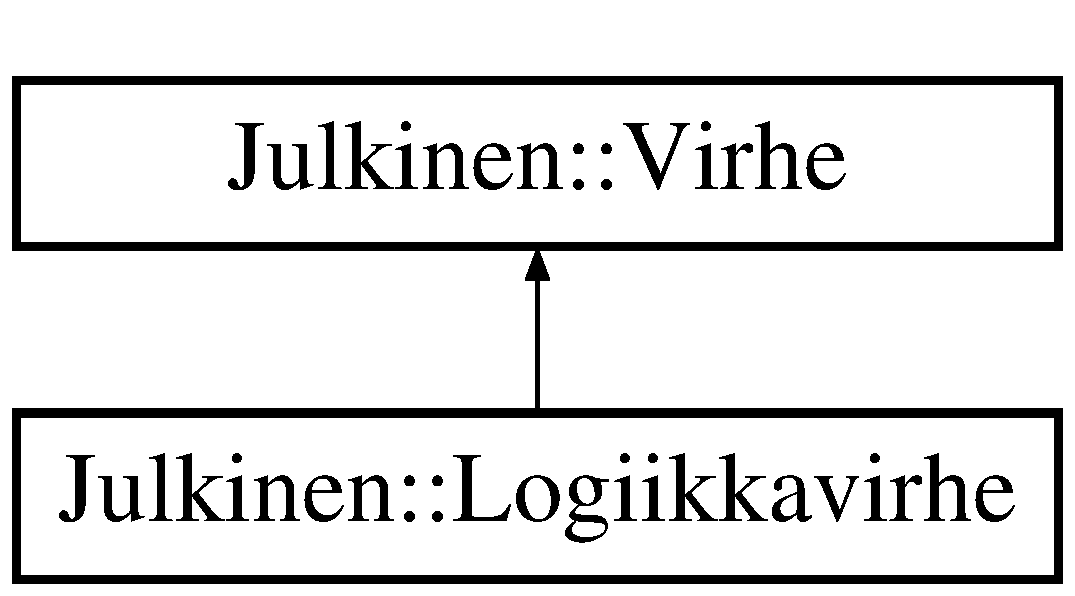
\includegraphics[height=2.000000cm]{class_julkinen_1_1_logiikkavirhe}
\end{center}
\end{figure}
\subsection*{Public Types}
\begin{DoxyCompactItemize}
\item 
enum \hyperlink{class_julkinen_1_1_logiikkavirhe_afbf716c9c72439df3d8638576942d14d}{Virhekoodi} \{ \hyperlink{class_julkinen_1_1_logiikkavirhe_afbf716c9c72439df3d8638576942d14da327478ab895f92a6e547db21b050ab8f}{V\+I\+R\+H\+E\+\_\+\+T\+U\+N\+N\+I\+S\+T\+A\+M\+A\+T\+O\+N}
 \}\begin{DoxyCompactList}\small\item\em Tunnisteet esimääritellyille virhetilanteille käyttäjän antamissa komennoissa. \end{DoxyCompactList}
\end{DoxyCompactItemize}
\subsection*{Public Member Functions}
\begin{DoxyCompactItemize}
\item 
\hyperlink{class_julkinen_1_1_logiikkavirhe_a95b0e31452062d57a34d5ee1e7b1545b}{Logiikkavirhe} (std\+::string const \&virheviesti)
\begin{DoxyCompactList}\small\item\em Tunnistamaton virhetilanne kopioidulla viestillä. \end{DoxyCompactList}\item 
\hyperlink{class_julkinen_1_1_logiikkavirhe_a82c17b4ae69d3701def7dee519b69024}{Logiikkavirhe} (\hyperlink{class_julkinen_1_1_logiikkavirhe_afbf716c9c72439df3d8638576942d14d}{Virhekoodi} virhekoodi)
\begin{DoxyCompactList}\small\item\em Esimääritelty virhetilanne. \end{DoxyCompactList}\item 
\hyperlink{class_julkinen_1_1_logiikkavirhe_a2ff42b2fc57b19638aebc7b8aa6f62d8}{Logiikkavirhe} (\hyperlink{class_julkinen_1_1_logiikkavirhe}{Logiikkavirhe} const \&toinen)
\begin{DoxyCompactList}\small\item\em Kopiorakentaja. \end{DoxyCompactList}\item 
\hyperlink{class_julkinen_1_1_logiikkavirhe}{Logiikkavirhe} \& \hyperlink{class_julkinen_1_1_logiikkavirhe_a9e680776140205960612e4b3b3be8e28}{operator=} (\hyperlink{class_julkinen_1_1_logiikkavirhe}{Logiikkavirhe} const \&toinen)
\begin{DoxyCompactList}\small\item\em Sijoitusoperaattori. \end{DoxyCompactList}\item 
\hyperlink{class_julkinen_1_1_logiikkavirhe_afbf716c9c72439df3d8638576942d14d}{Virhekoodi} \hyperlink{class_julkinen_1_1_logiikkavirhe_a453d06482aa51a80b27ab043d9efffaa}{virhe} () const 
\begin{DoxyCompactList}\small\item\em Sattuneen virhetilanteen virhekoodi. \end{DoxyCompactList}\item 
virtual std\+::basic\+\_\+ostream$<$ char $>$ \& \hyperlink{class_julkinen_1_1_logiikkavirhe_a298ce4b9c3d1887d5be431bea89645da}{tulosta} (std\+::basic\+\_\+ostream$<$ char $>$ \&tuloste) const 
\begin{DoxyCompactList}\small\item\em Tulosta virheen viesti virtaan. \end{DoxyCompactList}\end{DoxyCompactItemize}
\subsection*{Additional Inherited Members}


\subsection{Detailed Description}
\hyperlink{class_julkinen_1_1_virhe}{Virhe} toimintalogiikka virhetilanteita varten. 

\subsection{Member Enumeration Documentation}
\hypertarget{class_julkinen_1_1_logiikkavirhe_afbf716c9c72439df3d8638576942d14d}{}\index{Julkinen\+::\+Logiikkavirhe@{Julkinen\+::\+Logiikkavirhe}!Virhekoodi@{Virhekoodi}}
\index{Virhekoodi@{Virhekoodi}!Julkinen\+::\+Logiikkavirhe@{Julkinen\+::\+Logiikkavirhe}}
\subsubsection[{Virhekoodi}]{\setlength{\rightskip}{0pt plus 5cm}enum {\bf Julkinen\+::\+Logiikkavirhe\+::\+Virhekoodi}}\label{class_julkinen_1_1_logiikkavirhe_afbf716c9c72439df3d8638576942d14d}


Tunnisteet esimääritellyille virhetilanteille käyttäjän antamissa komennoissa. 

\begin{Desc}
\item[Enumerator]\par
\begin{description}
\index{V\+I\+R\+H\+E\+\_\+\+T\+U\+N\+N\+I\+S\+T\+A\+M\+A\+T\+O\+N@{V\+I\+R\+H\+E\+\_\+\+T\+U\+N\+N\+I\+S\+T\+A\+M\+A\+T\+O\+N}!Julkinen\+::\+Logiikkavirhe@{Julkinen\+::\+Logiikkavirhe}}\index{Julkinen\+::\+Logiikkavirhe@{Julkinen\+::\+Logiikkavirhe}!V\+I\+R\+H\+E\+\_\+\+T\+U\+N\+N\+I\+S\+T\+A\+M\+A\+T\+O\+N@{V\+I\+R\+H\+E\+\_\+\+T\+U\+N\+N\+I\+S\+T\+A\+M\+A\+T\+O\+N}}\item[{\em 
\hypertarget{class_julkinen_1_1_logiikkavirhe_afbf716c9c72439df3d8638576942d14da327478ab895f92a6e547db21b050ab8f}{}V\+I\+R\+H\+E\+\_\+\+T\+U\+N\+N\+I\+S\+T\+A\+M\+A\+T\+O\+N\label{class_julkinen_1_1_logiikkavirhe_afbf716c9c72439df3d8638576942d14da327478ab895f92a6e547db21b050ab8f}
}]Tunnistamaton virhe. \end{description}
\end{Desc}


\subsection{Constructor \& Destructor Documentation}
\hypertarget{class_julkinen_1_1_logiikkavirhe_a95b0e31452062d57a34d5ee1e7b1545b}{}\index{Julkinen\+::\+Logiikkavirhe@{Julkinen\+::\+Logiikkavirhe}!Logiikkavirhe@{Logiikkavirhe}}
\index{Logiikkavirhe@{Logiikkavirhe}!Julkinen\+::\+Logiikkavirhe@{Julkinen\+::\+Logiikkavirhe}}
\subsubsection[{Logiikkavirhe(std\+::string const \&virheviesti)}]{\setlength{\rightskip}{0pt plus 5cm}Logiikkavirhe\+::\+Logiikkavirhe (
\begin{DoxyParamCaption}
\item[{std\+::string const \&}]{virheviesti}
\end{DoxyParamCaption}
)\hspace{0.3cm}{\ttfamily [explicit]}}\label{class_julkinen_1_1_logiikkavirhe_a95b0e31452062d57a34d5ee1e7b1545b}


Tunnistamaton virhetilanne kopioidulla viestillä. 

Käytä tätä vain, jos kyseessä ei ole mikään esimääritellyistä virheistä.

\begin{DoxyPostcond}{Postcondition}
Perustakuu poikkeuksen sattuessa. 
\end{DoxyPostcond}

\begin{DoxyParams}{Parameters}
{\em virheviesti} & Merkkijono, joka kopioidaan poikkeuksen viestiksi. \\
\hline
\end{DoxyParams}

\begin{DoxyExceptions}{Exceptions}
{\em std\+::bad\+\_\+alloc} & Ei saatu varattua muistia viestiä varten. \\
\hline
\end{DoxyExceptions}
\hypertarget{class_julkinen_1_1_logiikkavirhe_a82c17b4ae69d3701def7dee519b69024}{}\index{Julkinen\+::\+Logiikkavirhe@{Julkinen\+::\+Logiikkavirhe}!Logiikkavirhe@{Logiikkavirhe}}
\index{Logiikkavirhe@{Logiikkavirhe}!Julkinen\+::\+Logiikkavirhe@{Julkinen\+::\+Logiikkavirhe}}
\subsubsection[{Logiikkavirhe(\+Virhekoodi virhekoodi)}]{\setlength{\rightskip}{0pt plus 5cm}Logiikkavirhe\+::\+Logiikkavirhe (
\begin{DoxyParamCaption}
\item[{{\bf Virhekoodi}}]{virhekoodi}
\end{DoxyParamCaption}
)\hspace{0.3cm}{\ttfamily [explicit]}}\label{class_julkinen_1_1_logiikkavirhe_a82c17b4ae69d3701def7dee519b69024}


Esimääritelty virhetilanne. 

\begin{DoxyPostcond}{Postcondition}
No-\/throw -\/takuu. 
\end{DoxyPostcond}

\begin{DoxyParams}{Parameters}
{\em virhekoodi} & Virhetilanteen tunniste. Mikäli koodi on V\+I\+R\+H\+E\+\_\+\+T\+U\+N\+N\+I\+S\+T\+A\+M\+A\+T\+O\+N, tulee viestiksi \char`\"{}\+Tunnistamaton virhe.\char`\"{}. \\
\hline
\end{DoxyParams}
\hypertarget{class_julkinen_1_1_logiikkavirhe_a2ff42b2fc57b19638aebc7b8aa6f62d8}{}\index{Julkinen\+::\+Logiikkavirhe@{Julkinen\+::\+Logiikkavirhe}!Logiikkavirhe@{Logiikkavirhe}}
\index{Logiikkavirhe@{Logiikkavirhe}!Julkinen\+::\+Logiikkavirhe@{Julkinen\+::\+Logiikkavirhe}}
\subsubsection[{Logiikkavirhe(\+Logiikkavirhe const \&toinen)}]{\setlength{\rightskip}{0pt plus 5cm}Logiikkavirhe\+::\+Logiikkavirhe (
\begin{DoxyParamCaption}
\item[{{\bf Logiikkavirhe} const \&}]{toinen}
\end{DoxyParamCaption}
)}\label{class_julkinen_1_1_logiikkavirhe_a2ff42b2fc57b19638aebc7b8aa6f62d8}


Kopiorakentaja. 

\begin{DoxyPostcond}{Postcondition}
No-\/throw -\/takuu. 
\end{DoxyPostcond}


\subsection{Member Function Documentation}
\hypertarget{class_julkinen_1_1_logiikkavirhe_a9e680776140205960612e4b3b3be8e28}{}\index{Julkinen\+::\+Logiikkavirhe@{Julkinen\+::\+Logiikkavirhe}!operator=@{operator=}}
\index{operator=@{operator=}!Julkinen\+::\+Logiikkavirhe@{Julkinen\+::\+Logiikkavirhe}}
\subsubsection[{operator=(\+Logiikkavirhe const \&toinen)}]{\setlength{\rightskip}{0pt plus 5cm}{\bf Logiikkavirhe} \& Logiikkavirhe\+::operator= (
\begin{DoxyParamCaption}
\item[{{\bf Logiikkavirhe} const \&}]{toinen}
\end{DoxyParamCaption}
)}\label{class_julkinen_1_1_logiikkavirhe_a9e680776140205960612e4b3b3be8e28}


Sijoitusoperaattori. 

\begin{DoxyPostcond}{Postcondition}
No-\/throw -\/takuu. 
\end{DoxyPostcond}
\hypertarget{class_julkinen_1_1_logiikkavirhe_a298ce4b9c3d1887d5be431bea89645da}{}\index{Julkinen\+::\+Logiikkavirhe@{Julkinen\+::\+Logiikkavirhe}!tulosta@{tulosta}}
\index{tulosta@{tulosta}!Julkinen\+::\+Logiikkavirhe@{Julkinen\+::\+Logiikkavirhe}}
\subsubsection[{tulosta(std\+::basic\+\_\+ostream$<$ char $>$ \&tuloste) const }]{\setlength{\rightskip}{0pt plus 5cm}basic\+\_\+ostream$<$ char $>$ \& Logiikkavirhe\+::tulosta (
\begin{DoxyParamCaption}
\item[{std\+::basic\+\_\+ostream$<$ char $>$ \&}]{tuloste}
\end{DoxyParamCaption}
) const\hspace{0.3cm}{\ttfamily [virtual]}}\label{class_julkinen_1_1_logiikkavirhe_a298ce4b9c3d1887d5be431bea89645da}


Tulosta virheen viesti virtaan. 

Tulostaa virheen viestin virtaan, eikä tee muuta.

\begin{DoxyPostcond}{Postcondition}
Vahva poikkeustakuu. 
\end{DoxyPostcond}

\begin{DoxyParams}{Parameters}
{\em tuloste} & Virta, jonne viesti tulostetaan. \\
\hline
\end{DoxyParams}
\begin{DoxyReturn}{Returns}
{\ttfamily tuloste} 
\end{DoxyReturn}


Reimplemented from \hyperlink{class_julkinen_1_1_virhe_a36a2644943038f9760b5d76a1960b00d}{Julkinen\+::\+Virhe}.

\hypertarget{class_julkinen_1_1_logiikkavirhe_a453d06482aa51a80b27ab043d9efffaa}{}\index{Julkinen\+::\+Logiikkavirhe@{Julkinen\+::\+Logiikkavirhe}!virhe@{virhe}}
\index{virhe@{virhe}!Julkinen\+::\+Logiikkavirhe@{Julkinen\+::\+Logiikkavirhe}}
\subsubsection[{virhe() const }]{\setlength{\rightskip}{0pt plus 5cm}{\bf Logiikkavirhe\+::\+Virhekoodi} Logiikkavirhe\+::virhe (
\begin{DoxyParamCaption}
{}
\end{DoxyParamCaption}
) const}\label{class_julkinen_1_1_logiikkavirhe_a453d06482aa51a80b27ab043d9efffaa}


Sattuneen virhetilanteen virhekoodi. 

\begin{DoxyReturn}{Returns}
Palauttaa virheen {\ttfamily Virhekoodi}. 
\end{DoxyReturn}


The documentation for this class was generated from the following files\+:\begin{DoxyCompactItemize}
\item 
\hyperlink{logiikkavirhe_8hh}{logiikkavirhe.\+hh}\item 
valmiiden\+\_\+toteutus/\hyperlink{logiikkavirhe_8cc}{logiikkavirhe.\+cc}\end{DoxyCompactItemize}

\hypertarget{class_naytto}{}\section{Naytto Class Reference}
\label{class_naytto}\index{Naytto@{Naytto}}


Labyrintti-\/pelin tulostusluokka.  




{\ttfamily \#include $<$naytto.\+hh$>$}

Inheritance diagram for Naytto\+:\begin{figure}[H]
\begin{center}
\leavevmode
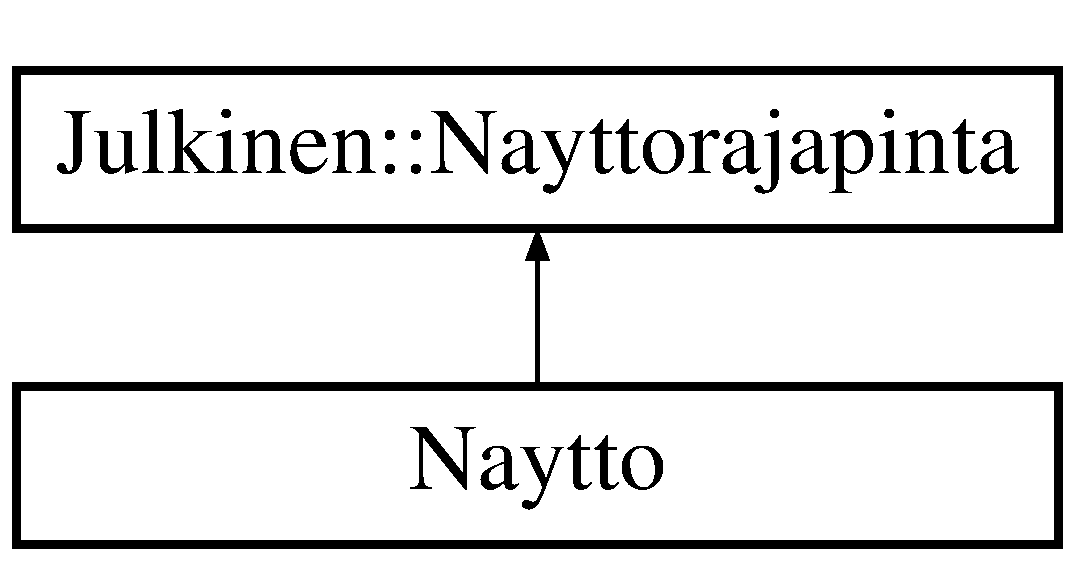
\includegraphics[height=2.000000cm]{class_naytto}
\end{center}
\end{figure}
\subsection*{Classes}
\begin{DoxyCompactItemize}
\item 
struct \hyperlink{struct_naytto_1_1_p}{P}
\begin{DoxyCompactList}\small\item\em Tulostuksessa avustava structi. \end{DoxyCompactList}\end{DoxyCompactItemize}
\subsection*{Public Member Functions}
\begin{DoxyCompactItemize}
\item 
\hyperlink{class_naytto_a10c88b8375ec0c4b88e55eb8005f1c9a}{Naytto} (\hyperlink{class_julkinen_1_1_koordinaatti}{Julkinen\+::\+Koordinaatti} const \&mitat, unsigned int x, unsigned int y, bool debug\+\_\+naytto)
\begin{DoxyCompactList}\small\item\em Näytönrakentaja. \end{DoxyCompactList}\item 
virtual \hyperlink{class_naytto_ac67aeac64dacc24f045210ab0b958768}{$\sim$\+Naytto} ()
\begin{DoxyCompactList}\small\item\em Purkaja. \end{DoxyCompactList}\item 
virtual bool \hyperlink{class_naytto_a1be5a43b84f00c279e6e8f619d613de9}{on\+Tulostustilassa} () const 
\begin{DoxyCompactList}\small\item\em Tulostustilan tarkistus. \end{DoxyCompactList}\item 
virtual void \hyperlink{class_naytto_a1ad6d3eea578c82c6260bc59d04e17a1}{ilmoitus\+Esine\+Poimittu} (char esine, std\+::string const \&pelaaja)
\item 
virtual void \hyperlink{class_naytto_ae8f3bdaee4c802e33be17b0efb50a530}{ilmoitus\+Erikoispalaan\+Astuttu} (\hyperlink{namespace_julkinen_afc26052e09d0b2214f749492cc5fff19}{Julkinen\+::\+Erikoispala\+Tyyppi} tyyppi, std\+::string const \&pelaaja)
\item 
virtual void \hyperlink{class_naytto_aebc53e0348c5f5ba88424a0e2a39991d}{ilmoitus\+Vuorossa} (std\+::string const \&nimi)
\begin{DoxyCompactList}\small\item\em Tulostaa tiedon vuorossa olevasta pelaajasta. \end{DoxyCompactList}\item 
virtual void \hyperlink{class_naytto_ababf9b69de2295fe4eaccc3d95461943}{tulosta\+Pelaajantiedot} (std\+::string const \&nimi, std\+::string const \&keratytesineet, std\+::string const \&kerattavatesineet, std\+::string const \&edellinentoiminto)
\item 
virtual void \hyperlink{class_naytto_a01a422be1ca30135634914767c8cd633}{komento\+Aloita\+Rakennus} ()
\begin{DoxyCompactList}\small\item\em Laittaa näytön pelialueen rakennustilaan. \end{DoxyCompactList}\item 
virtual void \hyperlink{class_naytto_adc11e0eddc17bfe1b9aa6971969b8549}{pala\+Laudalle} (\hyperlink{namespace_julkinen_a272c70e0503191a485c8a9cd4281e6f5}{Julkinen\+::\+Pala\+Tyyppi} tyyppi, \hyperlink{namespace_julkinen_afc26052e09d0b2214f749492cc5fff19}{Julkinen\+::\+Erikoispala\+Tyyppi} etyyppi, unsigned int rotaatio, \hyperlink{class_julkinen_1_1_koordinaatti}{Julkinen\+::\+Koordinaatti} const \&sijainti, \hyperlink{class_julkinen_1_1_koordinaatti}{Julkinen\+::\+Koordinaatti} const \&kohde=\hyperlink{class_julkinen_1_1_koordinaatti}{Julkinen\+::\+Koordinaatti}())
\item 
virtual void \hyperlink{class_naytto_a2425a87d92478b0c86ffe698985b6c86}{pelaaja\+Laudalle} (char merkki, \hyperlink{class_julkinen_1_1_koordinaatti}{Julkinen\+::\+Koordinaatti} const \&sijainti)
\item 
virtual void \hyperlink{class_naytto_a54c6a0f6fff0facbf4e769d77e80b341}{esine\+Laudalle} (char merkki, \hyperlink{class_julkinen_1_1_koordinaatti}{Julkinen\+::\+Koordinaatti} const \&sijainti)
\item 
virtual void \hyperlink{class_naytto_aa3faa1f5dde0249c90530f0fdfb25d7b}{komento\+Lopeta\+Rakennus} ()
\begin{DoxyCompactList}\small\item\em Lopeta laudanmuodostustila ja tulosta kartta, pelaajien tiedot ja irtopala. \end{DoxyCompactList}\item 
void \hyperlink{class_naytto_aeed4659324edc4f043ff43b2042de759}{tulosta} (std\+::ostringstream \&virta)
\begin{DoxyCompactList}\small\item\em Tulostaa virran. \end{DoxyCompactList}\item 
\hypertarget{class_naytto_a546211154c2e5fbfe30b3f329c3cdabe}{}void \hyperlink{class_naytto_a546211154c2e5fbfe30b3f329c3cdabe}{tulosta\+Voittaja} ()\label{class_naytto_a546211154c2e5fbfe30b3f329c3cdabe}

\begin{DoxyCompactList}\small\item\em Tulostaa ilmoituksen pelin voittajasta. \end{DoxyCompactList}\item 
void \hyperlink{class_naytto_a606d18d37a41a1dd32e7e837ce45d6ca}{vuorossa} ()
\begin{DoxyCompactList}\small\item\em Tulostaa vuorossa olevan pelaajan nimen ja kulman. \end{DoxyCompactList}\end{DoxyCompactItemize}


\subsection{Detailed Description}
Labyrintti-\/pelin tulostusluokka. 

\subsection{Constructor \& Destructor Documentation}
\hypertarget{class_naytto_a10c88b8375ec0c4b88e55eb8005f1c9a}{}\index{Naytto@{Naytto}!Naytto@{Naytto}}
\index{Naytto@{Naytto}!Naytto@{Naytto}}
\subsubsection[{Naytto(\+Julkinen\+::\+Koordinaatti const \&mitat, unsigned int x, unsigned int y, bool debug\+\_\+naytto)}]{\setlength{\rightskip}{0pt plus 5cm}Naytto\+::\+Naytto (
\begin{DoxyParamCaption}
\item[{{\bf Julkinen\+::\+Koordinaatti} const \&}]{mitat, }
\item[{unsigned int}]{x, }
\item[{unsigned int}]{y, }
\item[{bool}]{debug\+\_\+naytto}
\end{DoxyParamCaption}
)}\label{class_naytto_a10c88b8375ec0c4b88e55eb8005f1c9a}


Näytönrakentaja. 

Rakentaa näytön ja luo tarvittava {\ttfamily \hyperlink{class_bittikartta}{Bittikartta}} -\/oliot.


\begin{DoxyParams}[1]{Parameters}
\mbox{\tt in}  & {\em mitat} & Pelialueen koko {\ttfamily Koordinaatti}-\/luokkana. \\
\hline
\mbox{\tt in}  & {\em x} & {\ttfamily \hyperlink{class_bittikartta}{Bittikartta}} -\/olion leveys. \\
\hline
\mbox{\tt in}  & {\em y} & {\ttfamily \hyperlink{class_bittikartta}{Bittikartta}} -\/olion korkeus. \\
\hline
\end{DoxyParams}
\hypertarget{class_naytto_ac67aeac64dacc24f045210ab0b958768}{}\index{Naytto@{Naytto}!````~Naytto@{$\sim$\+Naytto}}
\index{````~Naytto@{$\sim$\+Naytto}!Naytto@{Naytto}}
\subsubsection[{$\sim$\+Naytto()}]{\setlength{\rightskip}{0pt plus 5cm}Naytto\+::$\sim$\+Naytto (
\begin{DoxyParamCaption}
{}
\end{DoxyParamCaption}
)\hspace{0.3cm}{\ttfamily [virtual]}}\label{class_naytto_ac67aeac64dacc24f045210ab0b958768}


Purkaja. 

\begin{DoxyPostcond}{Postcondition}
No-\/throw takuu. 
\end{DoxyPostcond}


\subsection{Member Function Documentation}
\hypertarget{class_naytto_a54c6a0f6fff0facbf4e769d77e80b341}{}\index{Naytto@{Naytto}!esine\+Laudalle@{esine\+Laudalle}}
\index{esine\+Laudalle@{esine\+Laudalle}!Naytto@{Naytto}}
\subsubsection[{esine\+Laudalle(char merkki, Julkinen\+::\+Koordinaatti const \&sijainti)}]{\setlength{\rightskip}{0pt plus 5cm}void Naytto\+::esine\+Laudalle (
\begin{DoxyParamCaption}
\item[{char}]{merkki, }
\item[{{\bf Julkinen\+::\+Koordinaatti} const \&}]{sijainti}
\end{DoxyParamCaption}
)\hspace{0.3cm}{\ttfamily [virtual]}}\label{class_naytto_a54c6a0f6fff0facbf4e769d77e80b341}




\begin{DoxyPrecond}{Precondition}
Nayttö on rakennustilassa. Esineen merkki, jokin \href{tyoohje.html}{\tt työohjeessa} annetuista merkeistä. Koordinaatti on pelialueen rajoissa.
\end{DoxyPrecond}
\begin{DoxyPostcond}{Postcondition}
\hyperlink{class_esine}{Esine} on lisätty tulostettavalle kartalle. Poikkeusturvallisuus\+: Perustakuu.
\end{DoxyPostcond}

\begin{DoxyParams}[1]{Parameters}
\mbox{\tt in}  & {\em merkki} & \hyperlink{class_esine}{Esine} sijaintia esittävä merkki kartalla. \\
\hline
\mbox{\tt in}  & {\em sijainti} & \hyperlink{class_esine}{Esine} koordinaatti kartalla. \\
\hline
\end{DoxyParams}


Implements \hyperlink{class_julkinen_1_1_nayttorajapinta_a64f3acc155ec834b7d8661fd7b85c50a}{Julkinen\+::\+Nayttorajapinta}.

\hypertarget{class_naytto_ae8f3bdaee4c802e33be17b0efb50a530}{}\index{Naytto@{Naytto}!ilmoitus\+Erikoispalaan\+Astuttu@{ilmoitus\+Erikoispalaan\+Astuttu}}
\index{ilmoitus\+Erikoispalaan\+Astuttu@{ilmoitus\+Erikoispalaan\+Astuttu}!Naytto@{Naytto}}
\subsubsection[{ilmoitus\+Erikoispalaan\+Astuttu(\+Julkinen\+::\+Erikoispala\+Tyyppi tyyppi, std\+::string const \&pelaaja)}]{\setlength{\rightskip}{0pt plus 5cm}void Naytto\+::ilmoitus\+Erikoispalaan\+Astuttu (
\begin{DoxyParamCaption}
\item[{{\bf Julkinen\+::\+Erikoispala\+Tyyppi}}]{tyyppi, }
\item[{std\+::string const \&}]{pelaaja}
\end{DoxyParamCaption}
)\hspace{0.3cm}{\ttfamily [virtual]}}\label{class_naytto_ae8f3bdaee4c802e33be17b0efb50a530}




\begin{DoxyPrecond}{Precondition}
Näyttö on tulostustilassa. 
\end{DoxyPrecond}
\begin{DoxyPostcond}{Postcondition}
Ilmoitus palaan astumisesta tehty. Poikkeusturvallisuus\+: Vahvatakuu, jos Nayttovirhe. Muuten perustakuu.
\end{DoxyPostcond}

\begin{DoxyParams}[1]{Parameters}
\mbox{\tt in}  & {\em tyyppi} & Erikoispalan \hyperlink{namespace_julkinen}{Julkinen}\+:Erikoispala\+Tyyppi \\
\hline
\mbox{\tt in}  & {\em pelaaja} & Pelaajan nimi, joka astui erikoispalaan\\
\hline
\end{DoxyParams}

\begin{DoxyExceptions}{Exceptions}
{\em Nayttovirhe} & Tulostus epäonnistui \\
\hline
\end{DoxyExceptions}


Implements \hyperlink{class_julkinen_1_1_nayttorajapinta_a9211bba3c7c7ed215752b8e311a5253f}{Julkinen\+::\+Nayttorajapinta}.

\hypertarget{class_naytto_a1ad6d3eea578c82c6260bc59d04e17a1}{}\index{Naytto@{Naytto}!ilmoitus\+Esine\+Poimittu@{ilmoitus\+Esine\+Poimittu}}
\index{ilmoitus\+Esine\+Poimittu@{ilmoitus\+Esine\+Poimittu}!Naytto@{Naytto}}
\subsubsection[{ilmoitus\+Esine\+Poimittu(char esine, std\+::string const \&pelaaja)}]{\setlength{\rightskip}{0pt plus 5cm}void Naytto\+::ilmoitus\+Esine\+Poimittu (
\begin{DoxyParamCaption}
\item[{char}]{esine, }
\item[{std\+::string const \&}]{pelaaja}
\end{DoxyParamCaption}
)\hspace{0.3cm}{\ttfamily [virtual]}}\label{class_naytto_a1ad6d3eea578c82c6260bc59d04e17a1}






Implements \hyperlink{class_julkinen_1_1_nayttorajapinta_afba451435164e30b22bd3060cdb09547}{Julkinen\+::\+Nayttorajapinta}.

\hypertarget{class_naytto_aebc53e0348c5f5ba88424a0e2a39991d}{}\index{Naytto@{Naytto}!ilmoitus\+Vuorossa@{ilmoitus\+Vuorossa}}
\index{ilmoitus\+Vuorossa@{ilmoitus\+Vuorossa}!Naytto@{Naytto}}
\subsubsection[{ilmoitus\+Vuorossa(std\+::string const \&nimi)}]{\setlength{\rightskip}{0pt plus 5cm}void Naytto\+::ilmoitus\+Vuorossa (
\begin{DoxyParamCaption}
\item[{std\+::string const \&}]{nimi}
\end{DoxyParamCaption}
)\hspace{0.3cm}{\ttfamily [virtual]}}\label{class_naytto_aebc53e0348c5f5ba88424a0e2a39991d}


Tulostaa tiedon vuorossa olevasta pelaajasta. 

Tulostaa vuorossa olevan pelaajan nimen ja $>$ merkin sen jälkeen. Metodi pitää ajaa Pelirajapinta\+::vaihda\+Vuoro() -\/metodi ajon jälkeen ja aina kun pelaajan antamassa komennossa on virhe.

\begin{DoxyPrecond}{Precondition}
Näyttö tulostustilassa 
\end{DoxyPrecond}
\begin{DoxyPostcond}{Postcondition}
Vuorossa olevan pelaajan nimi tulostettu. Poikkeustuvallisuus\+: Vahvatakuu, jos Nayttovirhe. Muuten perustakuu.
\end{DoxyPostcond}

\begin{DoxyParams}[1]{Parameters}
\mbox{\tt in}  & {\em nimi} & Vuorossa olevan pelaajan nimi.\\
\hline
\end{DoxyParams}

\begin{DoxyExceptions}{Exceptions}
{\em Nayttovirhe} & Tulostus epäonnistui. \\
\hline
\end{DoxyExceptions}


Implements \hyperlink{class_julkinen_1_1_nayttorajapinta_a9c54e560196f0c7e001d8fa5ee3533f2}{Julkinen\+::\+Nayttorajapinta}.

\hypertarget{class_naytto_a01a422be1ca30135634914767c8cd633}{}\index{Naytto@{Naytto}!komento\+Aloita\+Rakennus@{komento\+Aloita\+Rakennus}}
\index{komento\+Aloita\+Rakennus@{komento\+Aloita\+Rakennus}!Naytto@{Naytto}}
\subsubsection[{komento\+Aloita\+Rakennus()}]{\setlength{\rightskip}{0pt plus 5cm}void Naytto\+::komento\+Aloita\+Rakennus (
\begin{DoxyParamCaption}
{}
\end{DoxyParamCaption}
)\hspace{0.3cm}{\ttfamily [virtual]}}\label{class_naytto_a01a422be1ca30135634914767c8cd633}


Laittaa näytön pelialueen rakennustilaan. 

Asettaa näytön tilan rakennustilaan. Tämä metodi on ajettava ennen \hyperlink{class_naytto_adc11e0eddc17bfe1b9aa6971969b8549}{pala\+Laudalle()}, \hyperlink{class_naytto_a2425a87d92478b0c86ffe698985b6c86}{pelaaja\+Laudalle()}, \hyperlink{class_naytto_a54c6a0f6fff0facbf4e769d77e80b341}{esine\+Laudalle()} ja \hyperlink{class_naytto_aa3faa1f5dde0249c90530f0fdfb25d7b}{komento\+Lopeta\+Rakennus()} metodeja.

\begin{DoxyPrecond}{Precondition}
-\/ 
\end{DoxyPrecond}
\begin{DoxyPostcond}{Postcondition}
Näyttö on rakennustilassa ja pelilaudan kuva on tyhjä. Poikkeusturvallisuus\+: No-\/throw takuu. 
\end{DoxyPostcond}


Implements \hyperlink{class_julkinen_1_1_nayttorajapinta_a1a3335dcbda7cf2fb09f5e9319c42cea}{Julkinen\+::\+Nayttorajapinta}.

\hypertarget{class_naytto_aa3faa1f5dde0249c90530f0fdfb25d7b}{}\index{Naytto@{Naytto}!komento\+Lopeta\+Rakennus@{komento\+Lopeta\+Rakennus}}
\index{komento\+Lopeta\+Rakennus@{komento\+Lopeta\+Rakennus}!Naytto@{Naytto}}
\subsubsection[{komento\+Lopeta\+Rakennus()}]{\setlength{\rightskip}{0pt plus 5cm}void Naytto\+::komento\+Lopeta\+Rakennus (
\begin{DoxyParamCaption}
{}
\end{DoxyParamCaption}
)\hspace{0.3cm}{\ttfamily [virtual]}}\label{class_naytto_aa3faa1f5dde0249c90530f0fdfb25d7b}


Lopeta laudanmuodostustila ja tulosta kartta, pelaajien tiedot ja irtopala. 

\begin{DoxyPrecond}{Precondition}
Näyttö on rakennustilassa. 
\end{DoxyPrecond}
\begin{DoxyPostcond}{Postcondition}
Näyttörajapinta on tulostustilassa ja pelilauta on tulostettu. Poikkeusturvallisuus\+: Perustakuu.
\end{DoxyPostcond}

\begin{DoxyExceptions}{Exceptions}
{\em Nayttovirhe} & Tulostaminen epäonnistui. \\
\hline
\end{DoxyExceptions}


Implements \hyperlink{class_julkinen_1_1_nayttorajapinta_ab0fb18db1b26b45f898e0580dbbb8921}{Julkinen\+::\+Nayttorajapinta}.

\hypertarget{class_naytto_a1be5a43b84f00c279e6e8f619d613de9}{}\index{Naytto@{Naytto}!on\+Tulostustilassa@{on\+Tulostustilassa}}
\index{on\+Tulostustilassa@{on\+Tulostustilassa}!Naytto@{Naytto}}
\subsubsection[{on\+Tulostustilassa() const }]{\setlength{\rightskip}{0pt plus 5cm}bool Naytto\+::on\+Tulostustilassa (
\begin{DoxyParamCaption}
{}
\end{DoxyParamCaption}
) const\hspace{0.3cm}{\ttfamily [virtual]}}\label{class_naytto_a1be5a43b84f00c279e6e8f619d613de9}


Tulostustilan tarkistus. 

Kertoo näytön käyttäjälle onko näyttö tulostustilassa vai rakennustilassa. \begin{DoxyPrecond}{Precondition}
-\/ 
\end{DoxyPrecond}
\begin{DoxyPostcond}{Postcondition}
Palautettu tieto laudan tilasta. Poikkeusturvallisuus\+: No-\/throw takuu.
\end{DoxyPostcond}
\begin{DoxyReturn}{Returns}
{\ttfamily true} jos näyttö on tulostustilassa, {\ttfamily false} jos näyttö on rakennustilassa. 
\end{DoxyReturn}


Implements \hyperlink{class_julkinen_1_1_nayttorajapinta_ae4d4cc62685de755e51aade02cc05424}{Julkinen\+::\+Nayttorajapinta}.

\hypertarget{class_naytto_adc11e0eddc17bfe1b9aa6971969b8549}{}\index{Naytto@{Naytto}!pala\+Laudalle@{pala\+Laudalle}}
\index{pala\+Laudalle@{pala\+Laudalle}!Naytto@{Naytto}}
\subsubsection[{pala\+Laudalle(\+Julkinen\+::\+Pala\+Tyyppi tyyppi, Julkinen\+::\+Erikoispala\+Tyyppi etyyppi, unsigned int rotaatio, Julkinen\+::\+Koordinaatti const \&sijainti, Julkinen\+::\+Koordinaatti const \&kohde=\+Julkinen\+::\+Koordinaatti())}]{\setlength{\rightskip}{0pt plus 5cm}void Naytto\+::pala\+Laudalle (
\begin{DoxyParamCaption}
\item[{{\bf Julkinen\+::\+Pala\+Tyyppi}}]{tyyppi, }
\item[{{\bf Julkinen\+::\+Erikoispala\+Tyyppi}}]{etyyppi, }
\item[{unsigned int}]{rotaatio, }
\item[{{\bf Julkinen\+::\+Koordinaatti} const \&}]{sijainti, }
\item[{{\bf Julkinen\+::\+Koordinaatti} const \&}]{kohde = {\ttfamily {\bf Julkinen\+::\+Koordinaatti}()}}
\end{DoxyParamCaption}
)\hspace{0.3cm}{\ttfamily [virtual]}}\label{class_naytto_adc11e0eddc17bfe1b9aa6971969b8549}






Implements \hyperlink{class_julkinen_1_1_nayttorajapinta_aef4e3badfe7fa42dcfaba7bce4299301}{Julkinen\+::\+Nayttorajapinta}.

\hypertarget{class_naytto_a2425a87d92478b0c86ffe698985b6c86}{}\index{Naytto@{Naytto}!pelaaja\+Laudalle@{pelaaja\+Laudalle}}
\index{pelaaja\+Laudalle@{pelaaja\+Laudalle}!Naytto@{Naytto}}
\subsubsection[{pelaaja\+Laudalle(char merkki, Julkinen\+::\+Koordinaatti const \&sijainti)}]{\setlength{\rightskip}{0pt plus 5cm}void Naytto\+::pelaaja\+Laudalle (
\begin{DoxyParamCaption}
\item[{char}]{merkki, }
\item[{{\bf Julkinen\+::\+Koordinaatti} const \&}]{sijainti}
\end{DoxyParamCaption}
)\hspace{0.3cm}{\ttfamily [virtual]}}\label{class_naytto_a2425a87d92478b0c86ffe698985b6c86}




\begin{DoxyPrecond}{Precondition}
Nayttö on rakennustilassa. Koordinaatti on pelialueen rajoissa. 
\end{DoxyPrecond}
\begin{DoxyPostcond}{Postcondition}
\hyperlink{class_pelaaja}{Pelaaja} on lisätty tulostettavalle kartalle. Poikkeusturvallisuus\+: Perustakuu.
\end{DoxyPostcond}

\begin{DoxyParams}[1]{Parameters}
\mbox{\tt in}  & {\em merkki} & Pelaajan sijaintia esittävä merkki kartalla. \\
\hline
\mbox{\tt in}  & {\em sijainti} & Pelaajan koordinaatti kartalla. \\
\hline
\end{DoxyParams}


Implements \hyperlink{class_julkinen_1_1_nayttorajapinta_aa5db9bb4d55b723a2818fa0ec6ccd84a}{Julkinen\+::\+Nayttorajapinta}.

\hypertarget{class_naytto_aeed4659324edc4f043ff43b2042de759}{}\index{Naytto@{Naytto}!tulosta@{tulosta}}
\index{tulosta@{tulosta}!Naytto@{Naytto}}
\subsubsection[{tulosta(std\+::ostringstream \&virta)}]{\setlength{\rightskip}{0pt plus 5cm}void Naytto\+::tulosta (
\begin{DoxyParamCaption}
\item[{std\+::ostringstream \&}]{virta}
\end{DoxyParamCaption}
)}\label{class_naytto_aeed4659324edc4f043ff43b2042de759}


Tulostaa virran. 

Näyttö käyttää kaikeen tulostamiseen tätä funktiota.


\begin{DoxyParams}[1]{Parameters}
\mbox{\tt in}  & {\em virta} & Tulostettava virta. \\
\hline
\end{DoxyParams}
\hypertarget{class_naytto_ababf9b69de2295fe4eaccc3d95461943}{}\index{Naytto@{Naytto}!tulosta\+Pelaajantiedot@{tulosta\+Pelaajantiedot}}
\index{tulosta\+Pelaajantiedot@{tulosta\+Pelaajantiedot}!Naytto@{Naytto}}
\subsubsection[{tulosta\+Pelaajantiedot(std\+::string const \&nimi, std\+::string const \&keratytesineet, std\+::string const \&kerattavatesineet, std\+::string const \&edellinentoiminto)}]{\setlength{\rightskip}{0pt plus 5cm}void Naytto\+::tulosta\+Pelaajantiedot (
\begin{DoxyParamCaption}
\item[{std\+::string const \&}]{nimi, }
\item[{std\+::string const \&}]{keratytesineet, }
\item[{std\+::string const \&}]{kerattavatesineet, }
\item[{std\+::string const \&}]{edellinentoiminto}
\end{DoxyParamCaption}
)\hspace{0.3cm}{\ttfamily [virtual]}}\label{class_naytto_ababf9b69de2295fe4eaccc3d95461943}




\begin{DoxyPrecond}{Precondition}
Näyttö on on rakennustilassa. Pelaajan nimen pituus on \href{tyoohje.html}{\tt työohjeen} rajoissa. 
\end{DoxyPrecond}
\begin{DoxyPostcond}{Postcondition}
Pelaajan tiedot on lisätty tulostettavaksi. Poikkeusturvallisuus\+: Perustakuu.
\end{DoxyPostcond}

\begin{DoxyParams}[1]{Parameters}
\mbox{\tt in}  & {\em nimi} & Pelaajan, jonka tiedot tulostetaan, nimi. \\
\hline
\mbox{\tt in}  & {\em keratytesineet} & Pelaajan keräämät esineet. \\
\hline
\mbox{\tt in}  & {\em kerattavatesineet} & Pelaajan jäljellä olevat kerättävät esineet. \\
\hline
\mbox{\tt in}  & {\em edellinentoiminto} & Pelaajan edellinen toiminto. \\
\hline
\end{DoxyParams}


Implements \hyperlink{class_julkinen_1_1_nayttorajapinta_a22bcc0e0dc309960ad11a8bf232a87a7}{Julkinen\+::\+Nayttorajapinta}.

\hypertarget{class_naytto_a606d18d37a41a1dd32e7e837ce45d6ca}{}\index{Naytto@{Naytto}!vuorossa@{vuorossa}}
\index{vuorossa@{vuorossa}!Naytto@{Naytto}}
\subsubsection[{vuorossa()}]{\setlength{\rightskip}{0pt plus 5cm}void Naytto\+::vuorossa (
\begin{DoxyParamCaption}
{}
\end{DoxyParamCaption}
)}\label{class_naytto_a606d18d37a41a1dd32e7e837ce45d6ca}


Tulostaa vuorossa olevan pelaajan nimen ja kulman. 

\begin{DoxyPrecond}{Precondition}
\hyperlink{class_naytto_aebc53e0348c5f5ba88424a0e2a39991d}{ilmoitus\+Vuorossa()} metodi on ajettu ja naytto on tulostustilassa. 
\end{DoxyPrecond}
\begin{DoxyPostcond}{Postcondition}
vuorossa olevan pelaajan nimi ja kulma on tulostettu. 
\end{DoxyPostcond}


The documentation for this class was generated from the following files\+:\begin{DoxyCompactItemize}
\item 
valmiiden\+\_\+toteutus/include/\hyperlink{naytto_8hh}{naytto.\+hh}\item 
valmiiden\+\_\+toteutus/\hyperlink{naytto_8cc}{naytto.\+cc}\end{DoxyCompactItemize}

\hypertarget{class_julkinen_1_1_nayttorajapinta}{}\section{Julkinen\+:\+:Nayttorajapinta Class Reference}
\label{class_julkinen_1_1_nayttorajapinta}\index{Julkinen\+::\+Nayttorajapinta@{Julkinen\+::\+Nayttorajapinta}}


Labyrintti-\/pelin tulostusrajapinta.  




{\ttfamily \#include $<$nayttorajapinta.\+hh$>$}

Inheritance diagram for Julkinen\+:\+:Nayttorajapinta\+:\begin{figure}[H]
\begin{center}
\leavevmode
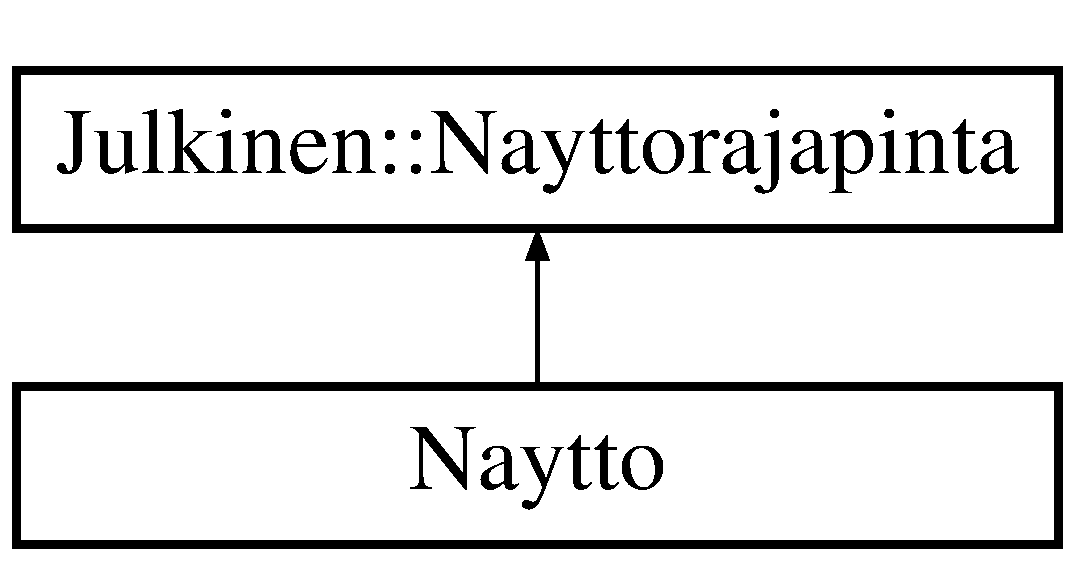
\includegraphics[height=2.000000cm]{class_julkinen_1_1_nayttorajapinta}
\end{center}
\end{figure}
\subsection*{Public Member Functions}
\begin{DoxyCompactItemize}
\item 
\hyperlink{class_julkinen_1_1_nayttorajapinta_a65c9201e902d59cdb9a089ca74670bf7}{Nayttorajapinta} ()
\begin{DoxyCompactList}\small\item\em Oletusrakentaja. \end{DoxyCompactList}\item 
virtual \hyperlink{class_julkinen_1_1_nayttorajapinta_ac38d827aa661d9c77fccb22b9bf25c9f}{$\sim$\+Nayttorajapinta} ()
\begin{DoxyCompactList}\small\item\em Oletuspurkaja. \end{DoxyCompactList}\item 
virtual bool \hyperlink{class_julkinen_1_1_nayttorajapinta_ae4d4cc62685de755e51aade02cc05424}{on\+Tulostustilassa} () const  =0
\begin{DoxyCompactList}\small\item\em Tulostustilan tarkistus. \end{DoxyCompactList}\item 
virtual void \hyperlink{class_julkinen_1_1_nayttorajapinta_afba451435164e30b22bd3060cdb09547}{ilmoitus\+Esine\+Poimittu} (char esine, std\+::string const \&pelaaja)=0
\begin{DoxyCompactList}\small\item\em Tulostaa ilmoituksen esineen poimisesta. \end{DoxyCompactList}\item 
virtual void \hyperlink{class_julkinen_1_1_nayttorajapinta_a9211bba3c7c7ed215752b8e311a5253f}{ilmoitus\+Erikoispalaan\+Astuttu} (\hyperlink{namespace_julkinen_afc26052e09d0b2214f749492cc5fff19}{Julkinen\+::\+Erikoispala\+Tyyppi} tyyppi, std\+::string const \&pelaaja)=0
\begin{DoxyCompactList}\small\item\em Tulostaa ilmoituksen erikoispalaan astumisesta. Tulostaa ilmoituksen, jossa kerrotaan että annettu pelaaja on astunut erikoispalaan, jonka tyyppi on annettu. \end{DoxyCompactList}\item 
virtual void \hyperlink{class_julkinen_1_1_nayttorajapinta_a9c54e560196f0c7e001d8fa5ee3533f2}{ilmoitus\+Vuorossa} (std\+::string const \&nimi)=0
\begin{DoxyCompactList}\small\item\em Tulostaa tiedon vuorossa olevasta pelaajasta. \end{DoxyCompactList}\item 
virtual void \hyperlink{class_julkinen_1_1_nayttorajapinta_a22bcc0e0dc309960ad11a8bf232a87a7}{tulosta\+Pelaajantiedot} (std\+::string const \&nimi, std\+::string const \&keratytesineet, std\+::string const \&kerattavatesineet, std\+::string const \&edellinentoiminto)=0
\begin{DoxyCompactList}\small\item\em Lisää yksittäisen pelaajan tiedot kartan alle tulostusta varten. \end{DoxyCompactList}\item 
virtual void \hyperlink{class_julkinen_1_1_nayttorajapinta_a1a3335dcbda7cf2fb09f5e9319c42cea}{komento\+Aloita\+Rakennus} ()=0
\begin{DoxyCompactList}\small\item\em Laittaa näytön pelialueen rakennustilaan. \end{DoxyCompactList}\item 
virtual void \hyperlink{class_julkinen_1_1_nayttorajapinta_aef4e3badfe7fa42dcfaba7bce4299301}{pala\+Laudalle} (\hyperlink{namespace_julkinen_a272c70e0503191a485c8a9cd4281e6f5}{Julkinen\+::\+Pala\+Tyyppi} tyyppi, \hyperlink{namespace_julkinen_afc26052e09d0b2214f749492cc5fff19}{Julkinen\+::\+Erikoispala\+Tyyppi} etyyppi, unsigned int rotaatio, \hyperlink{class_julkinen_1_1_koordinaatti}{Julkinen\+::\+Koordinaatti} const \&sijainti, \hyperlink{class_julkinen_1_1_koordinaatti}{Julkinen\+::\+Koordinaatti} const \&kohde=\hyperlink{class_julkinen_1_1_koordinaatti}{Julkinen\+::\+Koordinaatti}())=0
\begin{DoxyCompactList}\small\item\em Lisää palan tulostettavaan karttaan. \end{DoxyCompactList}\item 
virtual void \hyperlink{class_julkinen_1_1_nayttorajapinta_aa5db9bb4d55b723a2818fa0ec6ccd84a}{pelaaja\+Laudalle} (char merkki, \hyperlink{class_julkinen_1_1_koordinaatti}{Julkinen\+::\+Koordinaatti} const \&sijainti)=0
\begin{DoxyCompactList}\small\item\em Lisää pelaajan merkin tulostettavaan karttaan. \end{DoxyCompactList}\item 
virtual void \hyperlink{class_julkinen_1_1_nayttorajapinta_a64f3acc155ec834b7d8661fd7b85c50a}{esine\+Laudalle} (char merkki, \hyperlink{class_julkinen_1_1_koordinaatti}{Julkinen\+::\+Koordinaatti} const \&sijainti)=0
\begin{DoxyCompactList}\small\item\em Lisää esineen tulostettavaan lautaan. \end{DoxyCompactList}\item 
virtual void \hyperlink{class_julkinen_1_1_nayttorajapinta_ab0fb18db1b26b45f898e0580dbbb8921}{komento\+Lopeta\+Rakennus} ()=0
\begin{DoxyCompactList}\small\item\em Lopeta laudanmuodostustila ja tulosta kartta, pelaajien tiedot ja irtopala. \end{DoxyCompactList}\end{DoxyCompactItemize}


\subsection{Detailed Description}
Labyrintti-\/pelin tulostusrajapinta. 

Labyrintti pelin toiminnalisuuden toteuttava kirjasto tekee kaikki tulostukset tämän rajapinnan läpi. Rajapinnan toteutus on pääohjelman vastuulla.

Nayttorajapinnan toteutus voi olla kahdessa eri tilassa, tulostustilassa tai rakennustilassa. Oletuksena näyttö on tulostustilassa, jossa näyttö tulostaa ilmoitukset ja tiedot. Kutsumalla \hyperlink{class_julkinen_1_1_nayttorajapinta_a1a3335dcbda7cf2fb09f5e9319c42cea}{komento\+Aloita\+Rakennus()} metodia näyttö siirtyy rakennustilaan. Rakennustilassa näyttö alkaa odottamaan pelialueen rakennusta. Pelialue rakennetaan kutsumalla \hyperlink{class_julkinen_1_1_nayttorajapinta_aef4e3badfe7fa42dcfaba7bce4299301}{pala\+Laudalle()}, \hyperlink{class_julkinen_1_1_nayttorajapinta_aa5db9bb4d55b723a2818fa0ec6ccd84a}{pelaaja\+Laudalle()} ja \hyperlink{class_julkinen_1_1_nayttorajapinta_a64f3acc155ec834b7d8661fd7b85c50a}{esine\+Laudalle()} -\/metodeja. Rakennus tilassa pitää kutsua myös \hyperlink{class_julkinen_1_1_nayttorajapinta_a22bcc0e0dc309960ad11a8bf232a87a7}{tulosta\+Pelaajantiedot()} -\/metodia jokaiselle pelaajalle. Pelialueen rakennus lopetetaan kutsumalla \hyperlink{class_julkinen_1_1_nayttorajapinta_ab0fb18db1b26b45f898e0580dbbb8921}{komento\+Lopeta\+Rakennus()} -\/metodia.

Kaikki ei No-\/throw metodit heittävät std\+::bad\+\_\+alloc poikkeuksen, jos muisti loppuu. bac\+\_\+alloc\+:n yhteydessä luokka tarjoaa minimitakuun. bad\+\_\+alloc saa vuotaa ulos, eli muistin loppumiseen ei tarvitse erikseen varautua. 

\subsection{Constructor \& Destructor Documentation}
\hypertarget{class_julkinen_1_1_nayttorajapinta_a65c9201e902d59cdb9a089ca74670bf7}{}\index{Julkinen\+::\+Nayttorajapinta@{Julkinen\+::\+Nayttorajapinta}!Nayttorajapinta@{Nayttorajapinta}}
\index{Nayttorajapinta@{Nayttorajapinta}!Julkinen\+::\+Nayttorajapinta@{Julkinen\+::\+Nayttorajapinta}}
\subsubsection[{Nayttorajapinta()}]{\setlength{\rightskip}{0pt plus 5cm}Julkinen\+::\+Nayttorajapinta\+::\+Nayttorajapinta (
\begin{DoxyParamCaption}
{}
\end{DoxyParamCaption}
)\hspace{0.3cm}{\ttfamily [inline]}}\label{class_julkinen_1_1_nayttorajapinta_a65c9201e902d59cdb9a089ca74670bf7}


Oletusrakentaja. 

Tämä on määritelty vain, jotta voitaisiin määritellä olion tila heti luomisen jälkeen. \begin{DoxyPrecond}{Precondition}
-\/ 
\end{DoxyPrecond}
\begin{DoxyPostcond}{Postcondition}
Näyttörajapinta on tulostustilassa. Poikkeustakuu\+: Poikkeuksen sattuessa Pelirajapinta-\/olion luontiepäonnistui, mistä syytä oliolla ei ole sisäistä tilaa jolle voisi antaa takuita 
\end{DoxyPostcond}
\hypertarget{class_julkinen_1_1_nayttorajapinta_ac38d827aa661d9c77fccb22b9bf25c9f}{}\index{Julkinen\+::\+Nayttorajapinta@{Julkinen\+::\+Nayttorajapinta}!````~Nayttorajapinta@{$\sim$\+Nayttorajapinta}}
\index{````~Nayttorajapinta@{$\sim$\+Nayttorajapinta}!Julkinen\+::\+Nayttorajapinta@{Julkinen\+::\+Nayttorajapinta}}
\subsubsection[{$\sim$\+Nayttorajapinta()}]{\setlength{\rightskip}{0pt plus 5cm}virtual Julkinen\+::\+Nayttorajapinta\+::$\sim$\+Nayttorajapinta (
\begin{DoxyParamCaption}
{}
\end{DoxyParamCaption}
)\hspace{0.3cm}{\ttfamily [inline]}, {\ttfamily [virtual]}}\label{class_julkinen_1_1_nayttorajapinta_ac38d827aa661d9c77fccb22b9bf25c9f}


Oletuspurkaja. 

\begin{DoxyPrecond}{Precondition}
-\/ 
\end{DoxyPrecond}
\begin{DoxyPostcond}{Postcondition}
No-\/throw -\/takuu. 
\end{DoxyPostcond}


\subsection{Member Function Documentation}
\hypertarget{class_julkinen_1_1_nayttorajapinta_a64f3acc155ec834b7d8661fd7b85c50a}{}\index{Julkinen\+::\+Nayttorajapinta@{Julkinen\+::\+Nayttorajapinta}!esine\+Laudalle@{esine\+Laudalle}}
\index{esine\+Laudalle@{esine\+Laudalle}!Julkinen\+::\+Nayttorajapinta@{Julkinen\+::\+Nayttorajapinta}}
\subsubsection[{esine\+Laudalle(char merkki, Julkinen\+::\+Koordinaatti const \&sijainti)=0}]{\setlength{\rightskip}{0pt plus 5cm}virtual void Julkinen\+::\+Nayttorajapinta\+::esine\+Laudalle (
\begin{DoxyParamCaption}
\item[{char}]{merkki, }
\item[{{\bf Julkinen\+::\+Koordinaatti} const \&}]{sijainti}
\end{DoxyParamCaption}
)\hspace{0.3cm}{\ttfamily [pure virtual]}}\label{class_julkinen_1_1_nayttorajapinta_a64f3acc155ec834b7d8661fd7b85c50a}


Lisää esineen tulostettavaan lautaan. 

\begin{DoxyPrecond}{Precondition}
Nayttö on rakennustilassa. Esineen merkki, jokin \href{tyoohje.html}{\tt työohjeessa} annetuista merkeistä. \hyperlink{class_julkinen_1_1_koordinaatti}{Koordinaatti} on pelialueen rajoissa.
\end{DoxyPrecond}
\begin{DoxyPostcond}{Postcondition}
\hyperlink{class_esine}{Esine} on lisätty tulostettavalle kartalle. Poikkeusturvallisuus\+: Perustakuu.
\end{DoxyPostcond}

\begin{DoxyParams}[1]{Parameters}
\mbox{\tt in}  & {\em merkki} & \hyperlink{class_esine}{Esine} sijaintia esittävä merkki kartalla. \\
\hline
\mbox{\tt in}  & {\em sijainti} & \hyperlink{class_esine}{Esine} koordinaatti kartalla. \\
\hline
\end{DoxyParams}


Implemented in \hyperlink{class_naytto_a54c6a0f6fff0facbf4e769d77e80b341}{Naytto}.

\hypertarget{class_julkinen_1_1_nayttorajapinta_a9211bba3c7c7ed215752b8e311a5253f}{}\index{Julkinen\+::\+Nayttorajapinta@{Julkinen\+::\+Nayttorajapinta}!ilmoitus\+Erikoispalaan\+Astuttu@{ilmoitus\+Erikoispalaan\+Astuttu}}
\index{ilmoitus\+Erikoispalaan\+Astuttu@{ilmoitus\+Erikoispalaan\+Astuttu}!Julkinen\+::\+Nayttorajapinta@{Julkinen\+::\+Nayttorajapinta}}
\subsubsection[{ilmoitus\+Erikoispalaan\+Astuttu(\+Julkinen\+::\+Erikoispala\+Tyyppi tyyppi, std\+::string const \&pelaaja)=0}]{\setlength{\rightskip}{0pt plus 5cm}virtual void Julkinen\+::\+Nayttorajapinta\+::ilmoitus\+Erikoispalaan\+Astuttu (
\begin{DoxyParamCaption}
\item[{{\bf Julkinen\+::\+Erikoispala\+Tyyppi}}]{tyyppi, }
\item[{std\+::string const \&}]{pelaaja}
\end{DoxyParamCaption}
)\hspace{0.3cm}{\ttfamily [pure virtual]}}\label{class_julkinen_1_1_nayttorajapinta_a9211bba3c7c7ed215752b8e311a5253f}


Tulostaa ilmoituksen erikoispalaan astumisesta. Tulostaa ilmoituksen, jossa kerrotaan että annettu pelaaja on astunut erikoispalaan, jonka tyyppi on annettu. 

\begin{DoxyPrecond}{Precondition}
Näyttö on tulostustilassa. 
\end{DoxyPrecond}
\begin{DoxyPostcond}{Postcondition}
Ilmoitus palaan astumisesta tehty. Poikkeusturvallisuus\+: Vahvatakuu, jos \hyperlink{class_julkinen_1_1_nayttovirhe}{Nayttovirhe}. Muuten perustakuu.
\end{DoxyPostcond}

\begin{DoxyParams}[1]{Parameters}
\mbox{\tt in}  & {\em tyyppi} & Erikoispalan \hyperlink{namespace_julkinen}{Julkinen}\+:Erikoispala\+Tyyppi \\
\hline
\mbox{\tt in}  & {\em pelaaja} & Pelaajan nimi, joka astui erikoispalaan\\
\hline
\end{DoxyParams}

\begin{DoxyExceptions}{Exceptions}
{\em \hyperlink{class_julkinen_1_1_nayttovirhe}{Nayttovirhe}} & Tulostus epäonnistui \\
\hline
\end{DoxyExceptions}


Implemented in \hyperlink{class_naytto_ae8f3bdaee4c802e33be17b0efb50a530}{Naytto}.

\hypertarget{class_julkinen_1_1_nayttorajapinta_afba451435164e30b22bd3060cdb09547}{}\index{Julkinen\+::\+Nayttorajapinta@{Julkinen\+::\+Nayttorajapinta}!ilmoitus\+Esine\+Poimittu@{ilmoitus\+Esine\+Poimittu}}
\index{ilmoitus\+Esine\+Poimittu@{ilmoitus\+Esine\+Poimittu}!Julkinen\+::\+Nayttorajapinta@{Julkinen\+::\+Nayttorajapinta}}
\subsubsection[{ilmoitus\+Esine\+Poimittu(char esine, std\+::string const \&pelaaja)=0}]{\setlength{\rightskip}{0pt plus 5cm}virtual void Julkinen\+::\+Nayttorajapinta\+::ilmoitus\+Esine\+Poimittu (
\begin{DoxyParamCaption}
\item[{char}]{esine, }
\item[{std\+::string const \&}]{pelaaja}
\end{DoxyParamCaption}
)\hspace{0.3cm}{\ttfamily [pure virtual]}}\label{class_julkinen_1_1_nayttorajapinta_afba451435164e30b22bd3060cdb09547}


Tulostaa ilmoituksen esineen poimisesta. 

Tulostaa ilmoituksen jossa kerrotaan että annettu pelaaja on poiminut annetun esineen.

\begin{DoxyPrecond}{Precondition}
Näyttö tulostustilassa. 
\end{DoxyPrecond}
\begin{DoxyPostcond}{Postcondition}
Ilmoitus esineen poimisesta tehty. Poikkeusturvallisuus\+: Vahvatakuu, jos \hyperlink{class_julkinen_1_1_nayttovirhe}{Nayttovirhe}. Muuten perustakuu.
\end{DoxyPostcond}

\begin{DoxyParams}[1]{Parameters}
\mbox{\tt in}  & {\em esine} & Poimitun esineen merkki. \\
\hline
\mbox{\tt in}  & {\em pelaaja} & Pelaajan nimi, joka poimi esineen.\\
\hline
\end{DoxyParams}

\begin{DoxyExceptions}{Exceptions}
{\em \hyperlink{class_julkinen_1_1_nayttovirhe}{Nayttovirhe}} & Tulostus epäonnistui. \\
\hline
\end{DoxyExceptions}


Implemented in \hyperlink{class_naytto_a1ad6d3eea578c82c6260bc59d04e17a1}{Naytto}.

\hypertarget{class_julkinen_1_1_nayttorajapinta_a9c54e560196f0c7e001d8fa5ee3533f2}{}\index{Julkinen\+::\+Nayttorajapinta@{Julkinen\+::\+Nayttorajapinta}!ilmoitus\+Vuorossa@{ilmoitus\+Vuorossa}}
\index{ilmoitus\+Vuorossa@{ilmoitus\+Vuorossa}!Julkinen\+::\+Nayttorajapinta@{Julkinen\+::\+Nayttorajapinta}}
\subsubsection[{ilmoitus\+Vuorossa(std\+::string const \&nimi)=0}]{\setlength{\rightskip}{0pt plus 5cm}virtual void Julkinen\+::\+Nayttorajapinta\+::ilmoitus\+Vuorossa (
\begin{DoxyParamCaption}
\item[{std\+::string const \&}]{nimi}
\end{DoxyParamCaption}
)\hspace{0.3cm}{\ttfamily [pure virtual]}}\label{class_julkinen_1_1_nayttorajapinta_a9c54e560196f0c7e001d8fa5ee3533f2}


Tulostaa tiedon vuorossa olevasta pelaajasta. 

Tulostaa vuorossa olevan pelaajan nimen ja $>$ merkin sen jälkeen. Metodi pitää ajaa \hyperlink{class_julkinen_1_1_pelirajapinta_a873b4d57d698b82df131246df85c3193}{Pelirajapinta\+::vaihda\+Vuoro()} -\/metodi ajon jälkeen ja aina kun pelaajan antamassa komennossa on virhe.

\begin{DoxyPrecond}{Precondition}
Näyttö tulostustilassa 
\end{DoxyPrecond}
\begin{DoxyPostcond}{Postcondition}
Vuorossa olevan pelaajan nimi tulostettu. Poikkeustuvallisuus\+: Vahvatakuu, jos \hyperlink{class_julkinen_1_1_nayttovirhe}{Nayttovirhe}. Muuten perustakuu.
\end{DoxyPostcond}

\begin{DoxyParams}[1]{Parameters}
\mbox{\tt in}  & {\em nimi} & Vuorossa olevan pelaajan nimi.\\
\hline
\end{DoxyParams}

\begin{DoxyExceptions}{Exceptions}
{\em \hyperlink{class_julkinen_1_1_nayttovirhe}{Nayttovirhe}} & Tulostus epäonnistui. \\
\hline
\end{DoxyExceptions}


Implemented in \hyperlink{class_naytto_aebc53e0348c5f5ba88424a0e2a39991d}{Naytto}.

\hypertarget{class_julkinen_1_1_nayttorajapinta_a1a3335dcbda7cf2fb09f5e9319c42cea}{}\index{Julkinen\+::\+Nayttorajapinta@{Julkinen\+::\+Nayttorajapinta}!komento\+Aloita\+Rakennus@{komento\+Aloita\+Rakennus}}
\index{komento\+Aloita\+Rakennus@{komento\+Aloita\+Rakennus}!Julkinen\+::\+Nayttorajapinta@{Julkinen\+::\+Nayttorajapinta}}
\subsubsection[{komento\+Aloita\+Rakennus()=0}]{\setlength{\rightskip}{0pt plus 5cm}virtual void Julkinen\+::\+Nayttorajapinta\+::komento\+Aloita\+Rakennus (
\begin{DoxyParamCaption}
{}
\end{DoxyParamCaption}
)\hspace{0.3cm}{\ttfamily [pure virtual]}}\label{class_julkinen_1_1_nayttorajapinta_a1a3335dcbda7cf2fb09f5e9319c42cea}


Laittaa näytön pelialueen rakennustilaan. 

Asettaa näytön tilan rakennustilaan. Tämä metodi on ajettava ennen \hyperlink{class_julkinen_1_1_nayttorajapinta_aef4e3badfe7fa42dcfaba7bce4299301}{pala\+Laudalle()}, \hyperlink{class_julkinen_1_1_nayttorajapinta_aa5db9bb4d55b723a2818fa0ec6ccd84a}{pelaaja\+Laudalle()}, \hyperlink{class_julkinen_1_1_nayttorajapinta_a64f3acc155ec834b7d8661fd7b85c50a}{esine\+Laudalle()} ja \hyperlink{class_julkinen_1_1_nayttorajapinta_ab0fb18db1b26b45f898e0580dbbb8921}{komento\+Lopeta\+Rakennus()} metodeja.

\begin{DoxyPrecond}{Precondition}
-\/ 
\end{DoxyPrecond}
\begin{DoxyPostcond}{Postcondition}
Näyttö on rakennustilassa ja pelilaudan kuva on tyhjä. Poikkeusturvallisuus\+: No-\/throw takuu. 
\end{DoxyPostcond}


Implemented in \hyperlink{class_naytto_a01a422be1ca30135634914767c8cd633}{Naytto}.

\hypertarget{class_julkinen_1_1_nayttorajapinta_ab0fb18db1b26b45f898e0580dbbb8921}{}\index{Julkinen\+::\+Nayttorajapinta@{Julkinen\+::\+Nayttorajapinta}!komento\+Lopeta\+Rakennus@{komento\+Lopeta\+Rakennus}}
\index{komento\+Lopeta\+Rakennus@{komento\+Lopeta\+Rakennus}!Julkinen\+::\+Nayttorajapinta@{Julkinen\+::\+Nayttorajapinta}}
\subsubsection[{komento\+Lopeta\+Rakennus()=0}]{\setlength{\rightskip}{0pt plus 5cm}virtual void Julkinen\+::\+Nayttorajapinta\+::komento\+Lopeta\+Rakennus (
\begin{DoxyParamCaption}
{}
\end{DoxyParamCaption}
)\hspace{0.3cm}{\ttfamily [pure virtual]}}\label{class_julkinen_1_1_nayttorajapinta_ab0fb18db1b26b45f898e0580dbbb8921}


Lopeta laudanmuodostustila ja tulosta kartta, pelaajien tiedot ja irtopala. 

\begin{DoxyPrecond}{Precondition}
Näyttö on rakennustilassa. 
\end{DoxyPrecond}
\begin{DoxyPostcond}{Postcondition}
Näyttörajapinta on tulostustilassa ja pelilauta on tulostettu. Poikkeusturvallisuus\+: Perustakuu.
\end{DoxyPostcond}

\begin{DoxyExceptions}{Exceptions}
{\em \hyperlink{class_julkinen_1_1_nayttovirhe}{Nayttovirhe}} & Tulostaminen epäonnistui. \\
\hline
\end{DoxyExceptions}


Implemented in \hyperlink{class_naytto_aa3faa1f5dde0249c90530f0fdfb25d7b}{Naytto}.

\hypertarget{class_julkinen_1_1_nayttorajapinta_ae4d4cc62685de755e51aade02cc05424}{}\index{Julkinen\+::\+Nayttorajapinta@{Julkinen\+::\+Nayttorajapinta}!on\+Tulostustilassa@{on\+Tulostustilassa}}
\index{on\+Tulostustilassa@{on\+Tulostustilassa}!Julkinen\+::\+Nayttorajapinta@{Julkinen\+::\+Nayttorajapinta}}
\subsubsection[{on\+Tulostustilassa() const  =0}]{\setlength{\rightskip}{0pt plus 5cm}virtual bool Julkinen\+::\+Nayttorajapinta\+::on\+Tulostustilassa (
\begin{DoxyParamCaption}
{}
\end{DoxyParamCaption}
) const\hspace{0.3cm}{\ttfamily [pure virtual]}}\label{class_julkinen_1_1_nayttorajapinta_ae4d4cc62685de755e51aade02cc05424}


Tulostustilan tarkistus. 

Kertoo näytön käyttäjälle onko näyttö tulostustilassa vai rakennustilassa. \begin{DoxyPrecond}{Precondition}
-\/ 
\end{DoxyPrecond}
\begin{DoxyPostcond}{Postcondition}
Palautettu tieto laudan tilasta. Poikkeusturvallisuus\+: No-\/throw takuu.
\end{DoxyPostcond}
\begin{DoxyReturn}{Returns}
{\ttfamily true} jos näyttö on tulostustilassa, {\ttfamily false} jos näyttö on rakennustilassa. 
\end{DoxyReturn}


Implemented in \hyperlink{class_naytto_a1be5a43b84f00c279e6e8f619d613de9}{Naytto}.

\hypertarget{class_julkinen_1_1_nayttorajapinta_aef4e3badfe7fa42dcfaba7bce4299301}{}\index{Julkinen\+::\+Nayttorajapinta@{Julkinen\+::\+Nayttorajapinta}!pala\+Laudalle@{pala\+Laudalle}}
\index{pala\+Laudalle@{pala\+Laudalle}!Julkinen\+::\+Nayttorajapinta@{Julkinen\+::\+Nayttorajapinta}}
\subsubsection[{pala\+Laudalle(\+Julkinen\+::\+Pala\+Tyyppi tyyppi, Julkinen\+::\+Erikoispala\+Tyyppi etyyppi, unsigned int rotaatio, Julkinen\+::\+Koordinaatti const \&sijainti, Julkinen\+::\+Koordinaatti const \&kohde=\+Julkinen\+::\+Koordinaatti())=0}]{\setlength{\rightskip}{0pt plus 5cm}virtual void Julkinen\+::\+Nayttorajapinta\+::pala\+Laudalle (
\begin{DoxyParamCaption}
\item[{{\bf Julkinen\+::\+Pala\+Tyyppi}}]{tyyppi, }
\item[{{\bf Julkinen\+::\+Erikoispala\+Tyyppi}}]{etyyppi, }
\item[{unsigned int}]{rotaatio, }
\item[{{\bf Julkinen\+::\+Koordinaatti} const \&}]{sijainti, }
\item[{{\bf Julkinen\+::\+Koordinaatti} const \&}]{kohde = {\ttfamily {\bf Julkinen\+::\+Koordinaatti}()}}
\end{DoxyParamCaption}
)\hspace{0.3cm}{\ttfamily [pure virtual]}}\label{class_julkinen_1_1_nayttorajapinta_aef4e3badfe7fa42dcfaba7bce4299301}


Lisää palan tulostettavaan karttaan. 

\begin{DoxyPrecond}{Precondition}
Nayttö on rakennustilassa. \hyperlink{class_julkinen_1_1_koordinaatti}{Koordinaatti} on pelialueen rajoissa. Rotaatio on 1-\/4. 
\end{DoxyPrecond}
\begin{DoxyPostcond}{Postcondition}
\hyperlink{class_pala}{Pala} on lisatty tulostettavassa bittikartassa annettuun sijaintiin. Poikkeusturvallisuus\+: Perustakuu. 
\end{DoxyPostcond}

\begin{DoxyParams}[1]{Parameters}
\mbox{\tt in}  & {\em tyyppi} & Lisättävän palan tyyppi. \\
\hline
\mbox{\tt in}  & {\em etyyppi} & palaan liitetty \hyperlink{namespace_julkinen_afc26052e09d0b2214f749492cc5fff19}{Julkinen\+::\+Erikoispala\+Tyyppi}, käytetään -\/n vivun tulostuksen apuna. \\
\hline
\mbox{\tt in}  & {\em rotaatio} & Lisättävän palan rotaatio.\\
\hline
\mbox{\tt in}  & {\em sijainti} & koordinaatti mihin pala lisätään. Jos sijainti.\+onko\+Irtopala() palautaa {\ttfamily true}, niin palasta tehdään irtopala -\/kartta.\\
\hline
\mbox{\tt in}  & {\em kohde} & Teleporttipalan kohteen koordinaatti. Muilla paloilla parametria ei anneta. \\
\hline
\end{DoxyParams}


Implemented in \hyperlink{class_naytto_adc11e0eddc17bfe1b9aa6971969b8549}{Naytto}.

\hypertarget{class_julkinen_1_1_nayttorajapinta_aa5db9bb4d55b723a2818fa0ec6ccd84a}{}\index{Julkinen\+::\+Nayttorajapinta@{Julkinen\+::\+Nayttorajapinta}!pelaaja\+Laudalle@{pelaaja\+Laudalle}}
\index{pelaaja\+Laudalle@{pelaaja\+Laudalle}!Julkinen\+::\+Nayttorajapinta@{Julkinen\+::\+Nayttorajapinta}}
\subsubsection[{pelaaja\+Laudalle(char merkki, Julkinen\+::\+Koordinaatti const \&sijainti)=0}]{\setlength{\rightskip}{0pt plus 5cm}virtual void Julkinen\+::\+Nayttorajapinta\+::pelaaja\+Laudalle (
\begin{DoxyParamCaption}
\item[{char}]{merkki, }
\item[{{\bf Julkinen\+::\+Koordinaatti} const \&}]{sijainti}
\end{DoxyParamCaption}
)\hspace{0.3cm}{\ttfamily [pure virtual]}}\label{class_julkinen_1_1_nayttorajapinta_aa5db9bb4d55b723a2818fa0ec6ccd84a}


Lisää pelaajan merkin tulostettavaan karttaan. 

\begin{DoxyPrecond}{Precondition}
Nayttö on rakennustilassa. \hyperlink{class_julkinen_1_1_koordinaatti}{Koordinaatti} on pelialueen rajoissa. 
\end{DoxyPrecond}
\begin{DoxyPostcond}{Postcondition}
\hyperlink{class_pelaaja}{Pelaaja} on lisätty tulostettavalle kartalle. Poikkeusturvallisuus\+: Perustakuu.
\end{DoxyPostcond}

\begin{DoxyParams}[1]{Parameters}
\mbox{\tt in}  & {\em merkki} & Pelaajan sijaintia esittävä merkki kartalla. \\
\hline
\mbox{\tt in}  & {\em sijainti} & Pelaajan koordinaatti kartalla. \\
\hline
\end{DoxyParams}


Implemented in \hyperlink{class_naytto_a2425a87d92478b0c86ffe698985b6c86}{Naytto}.

\hypertarget{class_julkinen_1_1_nayttorajapinta_a22bcc0e0dc309960ad11a8bf232a87a7}{}\index{Julkinen\+::\+Nayttorajapinta@{Julkinen\+::\+Nayttorajapinta}!tulosta\+Pelaajantiedot@{tulosta\+Pelaajantiedot}}
\index{tulosta\+Pelaajantiedot@{tulosta\+Pelaajantiedot}!Julkinen\+::\+Nayttorajapinta@{Julkinen\+::\+Nayttorajapinta}}
\subsubsection[{tulosta\+Pelaajantiedot(std\+::string const \&nimi, std\+::string const \&keratytesineet, std\+::string const \&kerattavatesineet, std\+::string const \&edellinentoiminto)=0}]{\setlength{\rightskip}{0pt plus 5cm}virtual void Julkinen\+::\+Nayttorajapinta\+::tulosta\+Pelaajantiedot (
\begin{DoxyParamCaption}
\item[{std\+::string const \&}]{nimi, }
\item[{std\+::string const \&}]{keratytesineet, }
\item[{std\+::string const \&}]{kerattavatesineet, }
\item[{std\+::string const \&}]{edellinentoiminto}
\end{DoxyParamCaption}
)\hspace{0.3cm}{\ttfamily [pure virtual]}}\label{class_julkinen_1_1_nayttorajapinta_a22bcc0e0dc309960ad11a8bf232a87a7}


Lisää yksittäisen pelaajan tiedot kartan alle tulostusta varten. 

\begin{DoxyPrecond}{Precondition}
Näyttö on on rakennustilassa. Pelaajan nimen pituus on \href{tyoohje.html}{\tt työohjeen} rajoissa. 
\end{DoxyPrecond}
\begin{DoxyPostcond}{Postcondition}
Pelaajan tiedot on lisätty tulostettavaksi. Poikkeusturvallisuus\+: Perustakuu.
\end{DoxyPostcond}

\begin{DoxyParams}[1]{Parameters}
\mbox{\tt in}  & {\em nimi} & Pelaajan, jonka tiedot tulostetaan, nimi. \\
\hline
\mbox{\tt in}  & {\em keratytesineet} & Pelaajan keräämät esineet. \\
\hline
\mbox{\tt in}  & {\em kerattavatesineet} & Pelaajan jäljellä olevat kerättävät esineet. \\
\hline
\mbox{\tt in}  & {\em edellinentoiminto} & Pelaajan edellinen toiminto. \\
\hline
\end{DoxyParams}


Implemented in \hyperlink{class_naytto_ababf9b69de2295fe4eaccc3d95461943}{Naytto}.



The documentation for this class was generated from the following file\+:\begin{DoxyCompactItemize}
\item 
\hyperlink{nayttorajapinta_8hh}{nayttorajapinta.\+hh}\end{DoxyCompactItemize}

\hypertarget{class_julkinen_1_1_nayttovirhe}{}\section{Julkinen\+:\+:Nayttovirhe Class Reference}
\label{class_julkinen_1_1_nayttovirhe}\index{Julkinen\+::\+Nayttovirhe@{Julkinen\+::\+Nayttovirhe}}


Näyttörajapinnan tulostusoperaatio ei onnistunut.  




{\ttfamily \#include $<$nayttovirhe.\+hh$>$}

Inheritance diagram for Julkinen\+:\+:Nayttovirhe\+:\begin{figure}[H]
\begin{center}
\leavevmode
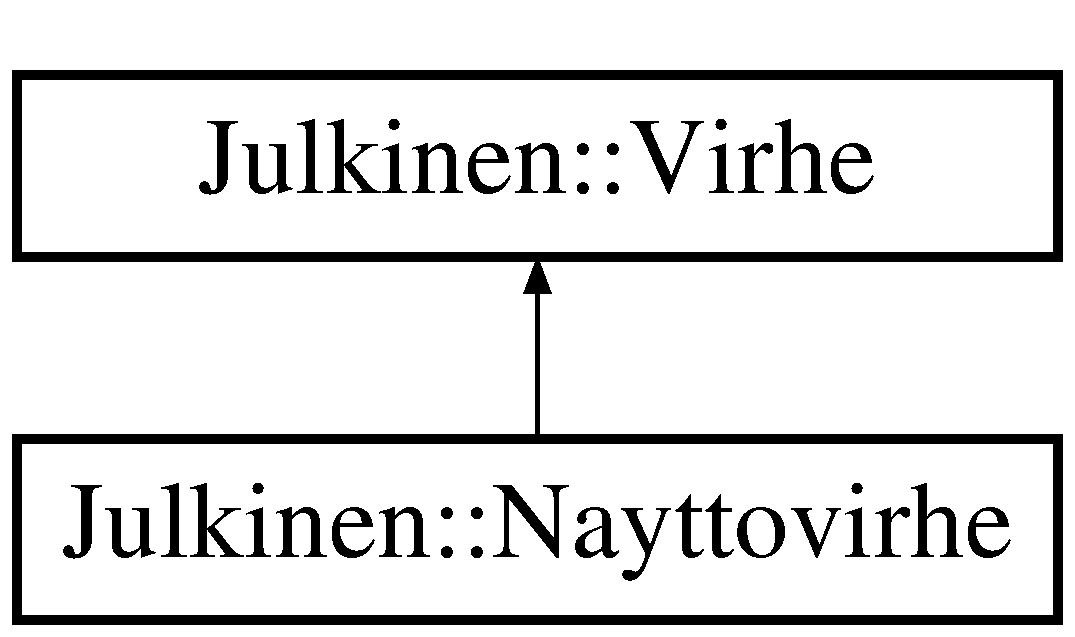
\includegraphics[height=2.000000cm]{class_julkinen_1_1_nayttovirhe}
\end{center}
\end{figure}
\subsection*{Public Types}
\begin{DoxyCompactItemize}
\item 
enum \hyperlink{class_julkinen_1_1_nayttovirhe_a13d43d49006dab024b0d3ac20a9fb8fa}{Virhekoodi} \{ \hyperlink{class_julkinen_1_1_nayttovirhe_a13d43d49006dab024b0d3ac20a9fb8faa26e7e527083430befdfdcd45f270514b}{V\+I\+R\+H\+E\+\_\+\+T\+U\+N\+N\+I\+S\+T\+A\+M\+A\+T\+O\+N}
 \}\begin{DoxyCompactList}\small\item\em Tunnisteet esimääritellyille virhetilanteille käyttäjän antamissa komennoissa. \end{DoxyCompactList}
\end{DoxyCompactItemize}
\subsection*{Public Member Functions}
\begin{DoxyCompactItemize}
\item 
\hyperlink{class_julkinen_1_1_nayttovirhe_a7e86d0fcc83269a4cfc34d487498e904}{Nayttovirhe} (std\+::string const \&virheviesti)
\begin{DoxyCompactList}\small\item\em Tunnistamaton virhetilanne kopioidulla viestillä. \end{DoxyCompactList}\item 
\hyperlink{class_julkinen_1_1_nayttovirhe_a02d21e4b5ddfdff5890742d05a0e81b7}{Nayttovirhe} (\hyperlink{class_julkinen_1_1_nayttovirhe_a13d43d49006dab024b0d3ac20a9fb8fa}{Virhekoodi} virhekoodi)
\begin{DoxyCompactList}\small\item\em Esimääritelty virhetilanne. \end{DoxyCompactList}\item 
\hyperlink{class_julkinen_1_1_nayttovirhe_a7765c49657111506d7b25a1720b21640}{Nayttovirhe} (\hyperlink{class_julkinen_1_1_nayttovirhe}{Nayttovirhe} const \&toinen)
\begin{DoxyCompactList}\small\item\em Kopiorakentaja. \end{DoxyCompactList}\item 
\hyperlink{class_julkinen_1_1_nayttovirhe}{Nayttovirhe} \& \hyperlink{class_julkinen_1_1_nayttovirhe_a3ced8ea4fdc6e72da15f6f480057c613}{operator=} (\hyperlink{class_julkinen_1_1_nayttovirhe}{Nayttovirhe} const \&toinen)
\begin{DoxyCompactList}\small\item\em Sijoitusoperaattori. \end{DoxyCompactList}\item 
\hyperlink{class_julkinen_1_1_nayttovirhe_a13d43d49006dab024b0d3ac20a9fb8fa}{Virhekoodi} \hyperlink{class_julkinen_1_1_nayttovirhe_a5ca5953148a213a4ffd79c191b0ab651}{virhe} () const 
\begin{DoxyCompactList}\small\item\em Sattuneen virhetilanteen virhekoodi. \end{DoxyCompactList}\item 
virtual std\+::basic\+\_\+ostream$<$ char $>$ \& \hyperlink{class_julkinen_1_1_nayttovirhe_ae8e4d0a5f98c3f61afc72dfed2af967f}{tulosta} (std\+::basic\+\_\+ostream$<$ char $>$ \&tuloste) const 
\begin{DoxyCompactList}\small\item\em Tulosta virheen viesti virtaan. \end{DoxyCompactList}\end{DoxyCompactItemize}
\subsection*{Additional Inherited Members}


\subsection{Detailed Description}
Näyttörajapinnan tulostusoperaatio ei onnistunut. 

\hyperlink{class_julkinen_1_1_virhe}{Virhe} jolla kerrotaan, jos näytön toiminnassa on tapahtunut jokin virhe 

\subsection{Member Enumeration Documentation}
\hypertarget{class_julkinen_1_1_nayttovirhe_a13d43d49006dab024b0d3ac20a9fb8fa}{}\index{Julkinen\+::\+Nayttovirhe@{Julkinen\+::\+Nayttovirhe}!Virhekoodi@{Virhekoodi}}
\index{Virhekoodi@{Virhekoodi}!Julkinen\+::\+Nayttovirhe@{Julkinen\+::\+Nayttovirhe}}
\subsubsection[{Virhekoodi}]{\setlength{\rightskip}{0pt plus 5cm}enum {\bf Julkinen\+::\+Nayttovirhe\+::\+Virhekoodi}}\label{class_julkinen_1_1_nayttovirhe_a13d43d49006dab024b0d3ac20a9fb8fa}


Tunnisteet esimääritellyille virhetilanteille käyttäjän antamissa komennoissa. 

\begin{Desc}
\item[Enumerator]\par
\begin{description}
\index{V\+I\+R\+H\+E\+\_\+\+T\+U\+N\+N\+I\+S\+T\+A\+M\+A\+T\+O\+N@{V\+I\+R\+H\+E\+\_\+\+T\+U\+N\+N\+I\+S\+T\+A\+M\+A\+T\+O\+N}!Julkinen\+::\+Nayttovirhe@{Julkinen\+::\+Nayttovirhe}}\index{Julkinen\+::\+Nayttovirhe@{Julkinen\+::\+Nayttovirhe}!V\+I\+R\+H\+E\+\_\+\+T\+U\+N\+N\+I\+S\+T\+A\+M\+A\+T\+O\+N@{V\+I\+R\+H\+E\+\_\+\+T\+U\+N\+N\+I\+S\+T\+A\+M\+A\+T\+O\+N}}\item[{\em 
\hypertarget{class_julkinen_1_1_nayttovirhe_a13d43d49006dab024b0d3ac20a9fb8faa26e7e527083430befdfdcd45f270514b}{}V\+I\+R\+H\+E\+\_\+\+T\+U\+N\+N\+I\+S\+T\+A\+M\+A\+T\+O\+N\label{class_julkinen_1_1_nayttovirhe_a13d43d49006dab024b0d3ac20a9fb8faa26e7e527083430befdfdcd45f270514b}
}]Tunnistamaton virhe. \end{description}
\end{Desc}


\subsection{Constructor \& Destructor Documentation}
\hypertarget{class_julkinen_1_1_nayttovirhe_a7e86d0fcc83269a4cfc34d487498e904}{}\index{Julkinen\+::\+Nayttovirhe@{Julkinen\+::\+Nayttovirhe}!Nayttovirhe@{Nayttovirhe}}
\index{Nayttovirhe@{Nayttovirhe}!Julkinen\+::\+Nayttovirhe@{Julkinen\+::\+Nayttovirhe}}
\subsubsection[{Nayttovirhe(std\+::string const \&virheviesti)}]{\setlength{\rightskip}{0pt plus 5cm}Nayttovirhe\+::\+Nayttovirhe (
\begin{DoxyParamCaption}
\item[{std\+::string const \&}]{virheviesti}
\end{DoxyParamCaption}
)\hspace{0.3cm}{\ttfamily [explicit]}}\label{class_julkinen_1_1_nayttovirhe_a7e86d0fcc83269a4cfc34d487498e904}


Tunnistamaton virhetilanne kopioidulla viestillä. 

Käytä tätä vain, jos kyseessä ei ole mikään esimääritellyistä virheistä.

\begin{DoxyPostcond}{Postcondition}
Perustakuu poikkeuksen sattuessa. 
\end{DoxyPostcond}

\begin{DoxyParams}{Parameters}
{\em virheviesti} & Merkkijono, joka kopioidaan poikkeuksen viestiksi. \\
\hline
\end{DoxyParams}

\begin{DoxyExceptions}{Exceptions}
{\em std\+::bad\+\_\+alloc} & Ei saatu varattua muistia viestiä varten. \\
\hline
\end{DoxyExceptions}
\hypertarget{class_julkinen_1_1_nayttovirhe_a02d21e4b5ddfdff5890742d05a0e81b7}{}\index{Julkinen\+::\+Nayttovirhe@{Julkinen\+::\+Nayttovirhe}!Nayttovirhe@{Nayttovirhe}}
\index{Nayttovirhe@{Nayttovirhe}!Julkinen\+::\+Nayttovirhe@{Julkinen\+::\+Nayttovirhe}}
\subsubsection[{Nayttovirhe(\+Virhekoodi virhekoodi)}]{\setlength{\rightskip}{0pt plus 5cm}Nayttovirhe\+::\+Nayttovirhe (
\begin{DoxyParamCaption}
\item[{{\bf Virhekoodi}}]{virhekoodi}
\end{DoxyParamCaption}
)\hspace{0.3cm}{\ttfamily [explicit]}}\label{class_julkinen_1_1_nayttovirhe_a02d21e4b5ddfdff5890742d05a0e81b7}


Esimääritelty virhetilanne. 

\begin{DoxyPostcond}{Postcondition}
No-\/throw -\/takuu. 
\end{DoxyPostcond}

\begin{DoxyParams}{Parameters}
{\em virhekoodi} & Virhetilanteen tunniste. Mikäli koodi on V\+I\+R\+H\+E\+\_\+\+T\+U\+N\+N\+I\+S\+T\+A\+M\+A\+T\+O\+N, tulee viestiksi \char`\"{}\+Tunnistamaton virhe.\char`\"{}. \\
\hline
\end{DoxyParams}
\hypertarget{class_julkinen_1_1_nayttovirhe_a7765c49657111506d7b25a1720b21640}{}\index{Julkinen\+::\+Nayttovirhe@{Julkinen\+::\+Nayttovirhe}!Nayttovirhe@{Nayttovirhe}}
\index{Nayttovirhe@{Nayttovirhe}!Julkinen\+::\+Nayttovirhe@{Julkinen\+::\+Nayttovirhe}}
\subsubsection[{Nayttovirhe(\+Nayttovirhe const \&toinen)}]{\setlength{\rightskip}{0pt plus 5cm}Nayttovirhe\+::\+Nayttovirhe (
\begin{DoxyParamCaption}
\item[{{\bf Nayttovirhe} const \&}]{toinen}
\end{DoxyParamCaption}
)}\label{class_julkinen_1_1_nayttovirhe_a7765c49657111506d7b25a1720b21640}


Kopiorakentaja. 

\begin{DoxyPostcond}{Postcondition}
No-\/throw -\/takuu. 
\end{DoxyPostcond}


\subsection{Member Function Documentation}
\hypertarget{class_julkinen_1_1_nayttovirhe_a3ced8ea4fdc6e72da15f6f480057c613}{}\index{Julkinen\+::\+Nayttovirhe@{Julkinen\+::\+Nayttovirhe}!operator=@{operator=}}
\index{operator=@{operator=}!Julkinen\+::\+Nayttovirhe@{Julkinen\+::\+Nayttovirhe}}
\subsubsection[{operator=(\+Nayttovirhe const \&toinen)}]{\setlength{\rightskip}{0pt plus 5cm}{\bf Nayttovirhe} \& Nayttovirhe\+::operator= (
\begin{DoxyParamCaption}
\item[{{\bf Nayttovirhe} const \&}]{toinen}
\end{DoxyParamCaption}
)}\label{class_julkinen_1_1_nayttovirhe_a3ced8ea4fdc6e72da15f6f480057c613}


Sijoitusoperaattori. 

\begin{DoxyPostcond}{Postcondition}
No-\/throw -\/takuu. 
\end{DoxyPostcond}
\hypertarget{class_julkinen_1_1_nayttovirhe_ae8e4d0a5f98c3f61afc72dfed2af967f}{}\index{Julkinen\+::\+Nayttovirhe@{Julkinen\+::\+Nayttovirhe}!tulosta@{tulosta}}
\index{tulosta@{tulosta}!Julkinen\+::\+Nayttovirhe@{Julkinen\+::\+Nayttovirhe}}
\subsubsection[{tulosta(std\+::basic\+\_\+ostream$<$ char $>$ \&tuloste) const }]{\setlength{\rightskip}{0pt plus 5cm}basic\+\_\+ostream$<$ char $>$ \& Nayttovirhe\+::tulosta (
\begin{DoxyParamCaption}
\item[{std\+::basic\+\_\+ostream$<$ char $>$ \&}]{tuloste}
\end{DoxyParamCaption}
) const\hspace{0.3cm}{\ttfamily [virtual]}}\label{class_julkinen_1_1_nayttovirhe_ae8e4d0a5f98c3f61afc72dfed2af967f}


Tulosta virheen viesti virtaan. 

Tulostaa virheen viestin virtaan, eikä tee muuta.

\begin{DoxyPostcond}{Postcondition}
Vahva poikkeustakuu. 
\end{DoxyPostcond}

\begin{DoxyParams}{Parameters}
{\em tuloste} & Virta, jonne viesti tulostetaan. \\
\hline
\end{DoxyParams}
\begin{DoxyReturn}{Returns}
{\ttfamily tuloste} 
\end{DoxyReturn}


Reimplemented from \hyperlink{class_julkinen_1_1_virhe_a36a2644943038f9760b5d76a1960b00d}{Julkinen\+::\+Virhe}.

\hypertarget{class_julkinen_1_1_nayttovirhe_a5ca5953148a213a4ffd79c191b0ab651}{}\index{Julkinen\+::\+Nayttovirhe@{Julkinen\+::\+Nayttovirhe}!virhe@{virhe}}
\index{virhe@{virhe}!Julkinen\+::\+Nayttovirhe@{Julkinen\+::\+Nayttovirhe}}
\subsubsection[{virhe() const }]{\setlength{\rightskip}{0pt plus 5cm}{\bf Nayttovirhe\+::\+Virhekoodi} Nayttovirhe\+::virhe (
\begin{DoxyParamCaption}
{}
\end{DoxyParamCaption}
) const}\label{class_julkinen_1_1_nayttovirhe_a5ca5953148a213a4ffd79c191b0ab651}


Sattuneen virhetilanteen virhekoodi. 

\begin{DoxyReturn}{Returns}
Palauttaa virheen {\ttfamily Virhekoodi}. 
\end{DoxyReturn}


The documentation for this class was generated from the following files\+:\begin{DoxyCompactItemize}
\item 
\hyperlink{nayttovirhe_8hh}{nayttovirhe.\+hh}\item 
valmiiden\+\_\+toteutus/\hyperlink{nayttovirhe_8cc}{nayttovirhe.\+cc}\end{DoxyCompactItemize}

\hypertarget{struct_naytto_1_1_p}{}\section{Naytto\+:\+:P Struct Reference}
\label{struct_naytto_1_1_p}\index{Naytto\+::\+P@{Naytto\+::\+P}}


Tulostuksessa avustava structi.  




{\ttfamily \#include $<$naytto.\+hh$>$}

\subsection*{Public Attributes}
\begin{DoxyCompactItemize}
\item 
\hypertarget{struct_naytto_1_1_p_a9929ca6c2e4bdfebf350522fee0e231a}{}std\+::string \hyperlink{struct_naytto_1_1_p_a9929ca6c2e4bdfebf350522fee0e231a}{yla}\label{struct_naytto_1_1_p_a9929ca6c2e4bdfebf350522fee0e231a}

\begin{DoxyCompactList}\small\item\em Palan ylälaitaa kuvaava merkkijono. \end{DoxyCompactList}\item 
\hypertarget{struct_naytto_1_1_p_a2476e4eb9177dff801da869a9ad010b3}{}std\+::string \hyperlink{struct_naytto_1_1_p_a2476e4eb9177dff801da869a9ad010b3}{oikea}\label{struct_naytto_1_1_p_a2476e4eb9177dff801da869a9ad010b3}

\begin{DoxyCompactList}\small\item\em Palan oikeaalaitaa kuvaava merkkijono. \end{DoxyCompactList}\item 
\hypertarget{struct_naytto_1_1_p_adbf8b79806a3b296be8f2867d0ca57df}{}std\+::string \hyperlink{struct_naytto_1_1_p_adbf8b79806a3b296be8f2867d0ca57df}{ala}\label{struct_naytto_1_1_p_adbf8b79806a3b296be8f2867d0ca57df}

\begin{DoxyCompactList}\small\item\em Palan alalaitaa kuvaava merkkijono. \end{DoxyCompactList}\item 
\hypertarget{struct_naytto_1_1_p_a66fa6f2d2fa48f179636a7d6321bbd9c}{}std\+::string \hyperlink{struct_naytto_1_1_p_a66fa6f2d2fa48f179636a7d6321bbd9c}{vasen}\label{struct_naytto_1_1_p_a66fa6f2d2fa48f179636a7d6321bbd9c}

\begin{DoxyCompactList}\small\item\em Palan vasentalaitaa kuvaava merkkijono. \end{DoxyCompactList}\end{DoxyCompactItemize}


\subsection{Detailed Description}
Tulostuksessa avustava structi. 

The documentation for this struct was generated from the following file\+:\begin{DoxyCompactItemize}
\item 
valmiiden\+\_\+toteutus/include/\hyperlink{naytto_8hh}{naytto.\+hh}\end{DoxyCompactItemize}

\hypertarget{class_pala}{}\section{Pala Class Reference}
\label{class_pala}\index{Pala@{Pala}}


Labyrintti-\/pelin palan tietoluokka.  




{\ttfamily \#include $<$Pala.\+hpp$>$}

\subsection*{Public Member Functions}
\begin{DoxyCompactItemize}
\item 
\hyperlink{class_pala_abfaef7049b3055dc7e3cc3ae93600dd8}{Pala} ()
\begin{DoxyCompactList}\small\item\em Palan tyhjä rakentaja. \end{DoxyCompactList}\item 
\hyperlink{class_pala_a45737786e7c2e42b097efac224117e4b}{Pala} (\hyperlink{namespace_julkinen_a272c70e0503191a485c8a9cd4281e6f5}{Julkinen\+::\+Pala\+Tyyppi} pala, unsigned int rotaatio, \hyperlink{class_julkinen_1_1_koordinaatti}{Julkinen\+::\+Koordinaatti} sijainti, \hyperlink{namespace_julkinen_afc26052e09d0b2214f749492cc5fff19}{Julkinen\+::\+Erikoispala\+Tyyppi} tyyppi=\hyperlink{namespace_julkinen_afc26052e09d0b2214f749492cc5fff19a67d9c76baa2a4eec4ca132c15bd567b5}{Julkinen\+::\+N\+O\+R\+M\+A\+A\+L\+I}, \hyperlink{class_julkinen_1_1_koordinaatti}{Julkinen\+::\+Koordinaatti} kohde=\hyperlink{class_julkinen_1_1_koordinaatti}{Julkinen\+::\+Koordinaatti}(), \hyperlink{class_esine}{Esine} $\ast$esine=N\+U\+L\+L, \hyperlink{class_pelaaja}{Pelaaja} $\ast$pelaaja=N\+U\+L\+L)
\begin{DoxyCompactList}\small\item\em Palan kuormitettu rakentaja. \end{DoxyCompactList}\item 
\hyperlink{class_pala_a86dec16c2dab10022d7fff922a568545}{$\sim$\+Pala} ()
\begin{DoxyCompactList}\small\item\em Purkaja. \end{DoxyCompactList}\item 
bool \hyperlink{class_pala_a80712cfbb26beb9a995ec78a0cf391b2}{keraa\+Esine} ()
\begin{DoxyCompactList}\small\item\em Esineen kerääjä \end{DoxyCompactList}\end{DoxyCompactItemize}
\subsection*{Public Attributes}
\begin{DoxyCompactItemize}
\item 
\hypertarget{class_pala_a800e05c778f3840d5b6cab3dc87f04af}{}\hyperlink{namespace_julkinen_a272c70e0503191a485c8a9cd4281e6f5}{Julkinen\+::\+Pala\+Tyyppi} {\bfseries pala}\label{class_pala_a800e05c778f3840d5b6cab3dc87f04af}

\item 
\hypertarget{class_pala_a0a0d1ef610c373bbd8f898cde6538a23}{}unsigned int {\bfseries rotaatio}\label{class_pala_a0a0d1ef610c373bbd8f898cde6538a23}

\item 
\hypertarget{class_pala_aa4ae7ca61e68d684389625b4e34ffa6b}{}\hyperlink{class_julkinen_1_1_koordinaatti}{Julkinen\+::\+Koordinaatti} {\bfseries sijainti}\label{class_pala_aa4ae7ca61e68d684389625b4e34ffa6b}

\item 
\hypertarget{class_pala_a48ddab2b6bdc1c541289d296bc8db7af}{}\hyperlink{namespace_julkinen_afc26052e09d0b2214f749492cc5fff19}{Julkinen\+::\+Erikoispala\+Tyyppi} {\bfseries tyyppi} = \hyperlink{namespace_julkinen_afc26052e09d0b2214f749492cc5fff19}{Julkinen\+::\+Erikoispala\+Tyyppi}()\label{class_pala_a48ddab2b6bdc1c541289d296bc8db7af}

\item 
\hypertarget{class_pala_acab51bd466aa1ff640683094d1eb0d20}{}\hyperlink{class_julkinen_1_1_koordinaatti}{Julkinen\+::\+Koordinaatti} {\bfseries kohde} = \hyperlink{class_julkinen_1_1_koordinaatti}{Julkinen\+::\+Koordinaatti}()\label{class_pala_acab51bd466aa1ff640683094d1eb0d20}

\item 
\hypertarget{class_pala_a35fceec264ac79f3ddf3c12a4e3cde1f}{}\hyperlink{class_esine}{Esine} $\ast$ {\bfseries esine} = N\+U\+L\+L\label{class_pala_a35fceec264ac79f3ddf3c12a4e3cde1f}

\item 
\hypertarget{class_pala_a9721ecfb8e78b412d5a6e0a72109e0e3}{}\hyperlink{class_pelaaja}{Pelaaja} $\ast$ {\bfseries pelaaja} = N\+U\+L\+L\label{class_pala_a9721ecfb8e78b412d5a6e0a72109e0e3}

\end{DoxyCompactItemize}


\subsection{Detailed Description}
Labyrintti-\/pelin palan tietoluokka. 

\subsection{Constructor \& Destructor Documentation}
\hypertarget{class_pala_abfaef7049b3055dc7e3cc3ae93600dd8}{}\index{Pala@{Pala}!Pala@{Pala}}
\index{Pala@{Pala}!Pala@{Pala}}
\subsubsection[{Pala()}]{\setlength{\rightskip}{0pt plus 5cm}Pala\+::\+Pala (
\begin{DoxyParamCaption}
{}
\end{DoxyParamCaption}
)}\label{class_pala_abfaef7049b3055dc7e3cc3ae93600dd8}


Palan tyhjä rakentaja. 

Alustaa muuttujat.

\begin{DoxyPostcond}{Postcondition}
Muuttujat on alustettu. 
\end{DoxyPostcond}
\hypertarget{class_pala_a45737786e7c2e42b097efac224117e4b}{}\index{Pala@{Pala}!Pala@{Pala}}
\index{Pala@{Pala}!Pala@{Pala}}
\subsubsection[{Pala(\+Julkinen\+::\+Pala\+Tyyppi pala, unsigned int rotaatio, Julkinen\+::\+Koordinaatti sijainti, Julkinen\+::\+Erikoispala\+Tyyppi tyyppi=\+Julkinen\+::\+N\+O\+R\+M\+A\+A\+L\+I, Julkinen\+::\+Koordinaatti kohde=\+Julkinen\+::\+Koordinaatti(), Esine $\ast$esine=\+N\+U\+L\+L, Pelaaja $\ast$pelaaja=\+N\+U\+L\+L)}]{\setlength{\rightskip}{0pt plus 5cm}Pala\+::\+Pala (
\begin{DoxyParamCaption}
\item[{{\bf Julkinen\+::\+Pala\+Tyyppi}}]{pala, }
\item[{unsigned int}]{rotaatio, }
\item[{{\bf Julkinen\+::\+Koordinaatti}}]{sijainti, }
\item[{{\bf Julkinen\+::\+Erikoispala\+Tyyppi}}]{tyyppi = {\ttfamily {\bf Julkinen\+::\+N\+O\+R\+M\+A\+A\+L\+I}}, }
\item[{{\bf Julkinen\+::\+Koordinaatti}}]{kohde = {\ttfamily {\bf Julkinen\+::\+Koordinaatti}()}, }
\item[{{\bf Esine} $\ast$}]{esine = {\ttfamily NULL}, }
\item[{{\bf Pelaaja} $\ast$}]{pelaaja = {\ttfamily NULL}}
\end{DoxyParamCaption}
)}\label{class_pala_a45737786e7c2e42b097efac224117e4b}


Palan kuormitettu rakentaja. 

Alustaa muuttujat annettuihin arvoihin.


\begin{DoxyParams}[1]{Parameters}
\mbox{\tt in}  & {\em pala} & Palan tyyppi {\ttfamily \hyperlink{namespace_julkinen_a272c70e0503191a485c8a9cd4281e6f5}{Julkinen\+::\+Pala\+Tyyppi}}-\/luokkana. \\
\hline
\mbox{\tt in}  & {\em rotaatio} & {\ttfamily Palan} rotaatio. \\
\hline
\mbox{\tt in}  & {\em sijainti} & Palan sijainti {\ttfamily \hyperlink{class_julkinen_1_1_koordinaatti}{Julkinen\+::\+Koordinaatti}}-\/luokkana. \\
\hline
\mbox{\tt in}  & {\em tyyppi} & Palan erikoispala tyyppi {\ttfamily \hyperlink{namespace_julkinen_afc26052e09d0b2214f749492cc5fff19}{Julkinen\+::\+Erikoispala\+Tyyppi}}-\/luokkana. \\
\hline
\mbox{\tt in}  & {\em kohde} & Palan kohde {\ttfamily \hyperlink{class_julkinen_1_1_koordinaatti}{Julkinen\+::\+Koordinaatti}}-\/luokkana. \\
\hline
\mbox{\tt in}  & {\em esine} & Palan esine {\ttfamily \hyperlink{class_esine}{Esine}}-\/luokkana. \\
\hline
\mbox{\tt in}  & {\em pelaaja} & Palan pelaaja {\ttfamily \hyperlink{class_pelaaja}{Pelaaja}}-\/luokkana.\\
\hline
\end{DoxyParams}
\begin{DoxyPostcond}{Postcondition}
Muuttujat on alustettu. 
\end{DoxyPostcond}
\hypertarget{class_pala_a86dec16c2dab10022d7fff922a568545}{}\index{Pala@{Pala}!````~Pala@{$\sim$\+Pala}}
\index{````~Pala@{$\sim$\+Pala}!Pala@{Pala}}
\subsubsection[{$\sim$\+Pala()}]{\setlength{\rightskip}{0pt plus 5cm}Pala\+::$\sim$\+Pala (
\begin{DoxyParamCaption}
{}
\end{DoxyParamCaption}
)}\label{class_pala_a86dec16c2dab10022d7fff922a568545}


Purkaja. 

\begin{DoxyPostcond}{Postcondition}
No-\/throw takuu. 
\end{DoxyPostcond}


\subsection{Member Function Documentation}
\hypertarget{class_pala_a80712cfbb26beb9a995ec78a0cf391b2}{}\index{Pala@{Pala}!keraa\+Esine@{keraa\+Esine}}
\index{keraa\+Esine@{keraa\+Esine}!Pala@{Pala}}
\subsubsection[{keraa\+Esine()}]{\setlength{\rightskip}{0pt plus 5cm}bool Pala\+::keraa\+Esine (
\begin{DoxyParamCaption}
{}
\end{DoxyParamCaption}
)}\label{class_pala_a80712cfbb26beb9a995ec78a0cf391b2}


Esineen kerääjä 

Tarkistaa voiko palalla istuva pelaaja kerätä esineen, jos sellaista on.

\begin{DoxyPrecond}{Precondition}
\hyperlink{class_esine}{Esine} on yritetty kerätä
\end{DoxyPrecond}
\begin{DoxyReturn}{Returns}
Palauttaa {\ttfamily true}, jos keräys onnistui. Palauttaa {\ttfamily false}, jos keräys epäonnistui. 
\end{DoxyReturn}


The documentation for this class was generated from the following files\+:\begin{DoxyCompactItemize}
\item 
\hyperlink{_pala_8hpp}{Pala.\+hpp}\item 
Pala.\+cpp\end{DoxyCompactItemize}

\hypertarget{class_pelaaja}{}\section{Pelaaja Class Reference}
\label{class_pelaaja}\index{Pelaaja@{Pelaaja}}


Labyrintti-\/pelin pelaajan tietoluokka.  




{\ttfamily \#include $<$Pelaaja.\+hpp$>$}

\subsection*{Public Member Functions}
\begin{DoxyCompactItemize}
\item 
\hyperlink{class_pelaaja_a278f63f50df4d765e6f0d9f7f69cb369}{Pelaaja} (\hyperlink{namespace_julkinen_ad9a0a9e01af78249f584a93b03db4329}{Julkinen\+::\+Pelaaja\+Tyyppi} \+\_\+tyyppi=\hyperlink{namespace_julkinen_ad9a0a9e01af78249f584a93b03db4329a72363d3abdcf0ff5a5318785a7d18363}{Julkinen\+::\+T\+I\+E\+T\+O\+K\+O\+N\+E}, std\+::string \+\_\+nimi=\char`\"{}\char`\"{}, char \+\_\+merkki= \textquotesingle{} \textquotesingle{}, std\+::queue$<$ \hyperlink{class_esine}{Esine} $\ast$ $>$ \+\_\+kerättävät\+Esineet=std\+::queue$<$ \hyperlink{class_esine}{Esine} $\ast$ $>$(), std\+::vector$<$ \hyperlink{class_esine}{Esine} $\ast$ $>$ \+\_\+keratyt\+Esineet=std\+::vector$<$ \hyperlink{class_esine}{Esine} $\ast$ $>$(), std\+::string \+\_\+edellinentoiminto=\char`\"{}\char`\"{}, bool \+\_\+extra\+Vuoro=false, bool \+\_\+meneta\+Vuoro=false, bool \+\_\+on\+Tyontanyt=false, bool \+\_\+on\+Liikkunut=false)
\begin{DoxyCompactList}\small\item\em Pelaajan kuormitettu rakentaja. \end{DoxyCompactList}\item 
\hyperlink{class_pelaaja_a60fe9baaf937de8fab8289f6bfc5e1ca}{$\sim$\+Pelaaja} ()
\begin{DoxyCompactList}\small\item\em Purkaja. \end{DoxyCompactList}\item 
std\+::string \hyperlink{class_pelaaja_af6d71411c2fb113bc8ae3c7ae0a7c2c7}{kerattavatesineet} ()
\begin{DoxyCompactList}\small\item\em Pelaajan kerättävien esineiden hakija. \end{DoxyCompactList}\item 
std\+::string \hyperlink{class_pelaaja_a65501bf1a3bb406261fcde36d1810c63}{keratytesineet} ()
\begin{DoxyCompactList}\small\item\em Pelaajan kerätyiden esineiden hakija. \end{DoxyCompactList}\end{DoxyCompactItemize}
\subsection*{Public Attributes}
\begin{DoxyCompactItemize}
\item 
\hypertarget{class_pelaaja_a02bdc32a1602c04fc09565dd798bc2ee}{}char {\bfseries merkki}\label{class_pelaaja_a02bdc32a1602c04fc09565dd798bc2ee}

\item 
\hypertarget{class_pelaaja_a8d801247c05210f893e2bea4581c2921}{}\hyperlink{namespace_julkinen_ad9a0a9e01af78249f584a93b03db4329}{Julkinen\+::\+Pelaaja\+Tyyppi} {\bfseries tyyppi}\label{class_pelaaja_a8d801247c05210f893e2bea4581c2921}

\item 
\hypertarget{class_pelaaja_aa078f73c51dbd0093a15ce3b13799355}{}std\+::string {\bfseries nimi}\label{class_pelaaja_aa078f73c51dbd0093a15ce3b13799355}

\item 
\hypertarget{class_pelaaja_aa4fca4902c77288a27d0924ca8232653}{}std\+::string {\bfseries edellinentoiminto}\label{class_pelaaja_aa4fca4902c77288a27d0924ca8232653}

\item 
\hypertarget{class_pelaaja_aed59d61a02879aee8e06bcf9444e1c7e}{}std\+::queue$<$ \hyperlink{class_esine}{Esine} $\ast$ $>$ {\bfseries kerättävät\+Esineet}\label{class_pelaaja_aed59d61a02879aee8e06bcf9444e1c7e}

\item 
\hypertarget{class_pelaaja_acdb0a8c22d4c7c53c6f37925166fa894}{}std\+::vector$<$ \hyperlink{class_esine}{Esine} $\ast$ $>$ {\bfseries keratyt\+Esineet}\label{class_pelaaja_acdb0a8c22d4c7c53c6f37925166fa894}

\item 
\hypertarget{class_pelaaja_a96e6bda620a26db66ccb5abe2dbc4014}{}bool {\bfseries extra\+Vuoro}\label{class_pelaaja_a96e6bda620a26db66ccb5abe2dbc4014}

\item 
\hypertarget{class_pelaaja_a6484c51c4abc90f56dcdff8c7ab4cbf6}{}bool {\bfseries meneta\+Vuoro}\label{class_pelaaja_a6484c51c4abc90f56dcdff8c7ab4cbf6}

\item 
\hypertarget{class_pelaaja_a0d5674f0d949024ccf3330fe074384f2}{}bool {\bfseries on\+Tyontanyt}\label{class_pelaaja_a0d5674f0d949024ccf3330fe074384f2}

\item 
\hypertarget{class_pelaaja_a55e8ede0cb70c5666158146ae563cef2}{}bool {\bfseries on\+Liikkunut}\label{class_pelaaja_a55e8ede0cb70c5666158146ae563cef2}

\end{DoxyCompactItemize}


\subsection{Detailed Description}
Labyrintti-\/pelin pelaajan tietoluokka. 

\subsection{Constructor \& Destructor Documentation}
\hypertarget{class_pelaaja_a278f63f50df4d765e6f0d9f7f69cb369}{}\index{Pelaaja@{Pelaaja}!Pelaaja@{Pelaaja}}
\index{Pelaaja@{Pelaaja}!Pelaaja@{Pelaaja}}
\subsubsection[{Pelaaja(\+Julkinen\+::\+Pelaaja\+Tyyppi \+\_\+tyyppi=\+Julkinen\+::\+T\+I\+E\+T\+O\+K\+O\+N\+E, std\+::string \+\_\+nimi="""", char \+\_\+merkki= \textquotesingle{} \textquotesingle{}, std\+::queue$<$ Esine $\ast$ $>$ \+\_\+kerättävät\+Esineet=std\+::queue$<$ Esine $\ast$ $>$(), std\+::vector$<$ Esine $\ast$ $>$ \+\_\+keratyt\+Esineet=std\+::vector$<$ Esine $\ast$ $>$(), std\+::string \+\_\+edellinentoiminto="""", bool \+\_\+extra\+Vuoro=false, bool \+\_\+meneta\+Vuoro=false, bool \+\_\+on\+Tyontanyt=false, bool \+\_\+on\+Liikkunut=false)}]{\setlength{\rightskip}{0pt plus 5cm}Pelaaja\+::\+Pelaaja (
\begin{DoxyParamCaption}
\item[{{\bf Julkinen\+::\+Pelaaja\+Tyyppi}}]{\+\_\+tyyppi = {\ttfamily {\bf Julkinen\+::\+T\+I\+E\+T\+O\+K\+O\+N\+E}}, }
\item[{std\+::string}]{\+\_\+nimi = {\ttfamily \char`\"{}\char`\"{}}, }
\item[{char}]{\+\_\+merkki = {\ttfamily \textquotesingle{}~\textquotesingle{}}, }
\item[{std\+::queue$<$ {\bf Esine} $\ast$ $>$}]{\+\_\+kerättävät\+Esineet = {\ttfamily std\+:\+:queue$<${\bf Esine}$\ast$$>$()}, }
\item[{std\+::vector$<$ {\bf Esine} $\ast$ $>$}]{\+\_\+keratyt\+Esineet = {\ttfamily std\+:\+:vector$<${\bf Esine}$\ast$$>$()}, }
\item[{std\+::string}]{\+\_\+edellinentoiminto = {\ttfamily \char`\"{}\char`\"{}}, }
\item[{bool}]{\+\_\+extra\+Vuoro = {\ttfamily false}, }
\item[{bool}]{\+\_\+meneta\+Vuoro = {\ttfamily false}, }
\item[{bool}]{\+\_\+on\+Tyontanyt = {\ttfamily false}, }
\item[{bool}]{\+\_\+on\+Liikkunut = {\ttfamily false}}
\end{DoxyParamCaption}
)}\label{class_pelaaja_a278f63f50df4d765e6f0d9f7f69cb369}


Pelaajan kuormitettu rakentaja. 

Alustaa muuttujat annettuihin arvoihin.


\begin{DoxyParams}[1]{Parameters}
\mbox{\tt in}  & {\em \+\_\+tyyppi} & Pelaajan tyyppi {\ttfamily \hyperlink{namespace_julkinen_ad9a0a9e01af78249f584a93b03db4329}{Julkinen\+::\+Pelaaja\+Tyyppi}}-\/luokkana. \\
\hline
\mbox{\tt in}  & {\em \+\_\+nimi} & {\ttfamily Pelaajan} nimi. \\
\hline
\mbox{\tt in}  & {\em \+\_\+merkki} & {\ttfamily Pelaajan} merkki. \\
\hline
\mbox{\tt in}  & {\em \+\_\+kerättävät\+Esineet} & Pelaajan kerättävät esineet {\ttfamily Julkinen\+::\+Esine}-\/luokka osoite jonona. \\
\hline
\mbox{\tt in}  & {\em \+\_\+kerättävät\+Esineet} & Pelaajan kerätyt esineet {\ttfamily Julkinen\+::\+Esine}-\/luokka osoite vektorina. \\
\hline
\mbox{\tt in}  & {\em \+\_\+edellinentoiminto} & {\ttfamily Pelaajan} edellinen toiminto. \\
\hline
\mbox{\tt in}  & {\em \+\_\+extra\+Vuoro} & {\ttfamily Tieto} pelaajan extra vuorosta {\ttfamily true} tai {\ttfamily false}. \\
\hline
\mbox{\tt in}  & {\em \+\_\+meneta\+Vuoro} & {\ttfamily Tieto} pelaajan menetetystä vuorosta {\ttfamily true} tai {\ttfamily false}. \\
\hline
\mbox{\tt in}  & {\em \+\_\+on\+Tyontanyt} & {\ttfamily Tieto} onko pelaaja työntänyt {\ttfamily true} tai {\ttfamily false}. \\
\hline
\mbox{\tt in}  & {\em \+\_\+on\+Liikkunut} & {\ttfamily Tieto} onko pelaaja liikkunut {\ttfamily true} tai {\ttfamily false}.\\
\hline
\end{DoxyParams}
\begin{DoxyPostcond}{Postcondition}
Muuttujat on alustettu. 
\end{DoxyPostcond}
\hypertarget{class_pelaaja_a60fe9baaf937de8fab8289f6bfc5e1ca}{}\index{Pelaaja@{Pelaaja}!````~Pelaaja@{$\sim$\+Pelaaja}}
\index{````~Pelaaja@{$\sim$\+Pelaaja}!Pelaaja@{Pelaaja}}
\subsubsection[{$\sim$\+Pelaaja()}]{\setlength{\rightskip}{0pt plus 5cm}Pelaaja\+::$\sim$\+Pelaaja (
\begin{DoxyParamCaption}
{}
\end{DoxyParamCaption}
)}\label{class_pelaaja_a60fe9baaf937de8fab8289f6bfc5e1ca}


Purkaja. 

\begin{DoxyPostcond}{Postcondition}
No-\/throw takuu. 
\end{DoxyPostcond}


\subsection{Member Function Documentation}
\hypertarget{class_pelaaja_af6d71411c2fb113bc8ae3c7ae0a7c2c7}{}\index{Pelaaja@{Pelaaja}!kerattavatesineet@{kerattavatesineet}}
\index{kerattavatesineet@{kerattavatesineet}!Pelaaja@{Pelaaja}}
\subsubsection[{kerattavatesineet()}]{\setlength{\rightskip}{0pt plus 5cm}std\+::string Pelaaja\+::kerattavatesineet (
\begin{DoxyParamCaption}
{}
\end{DoxyParamCaption}
)}\label{class_pelaaja_af6d71411c2fb113bc8ae3c7ae0a7c2c7}


Pelaajan kerättävien esineiden hakija. 

Hakee muotoillun std\+::string muuttujan kerättäviestä esineistä.

\begin{DoxyPostcond}{Postcondition}
Muotoiltu std\+::string muuttuja on luotu ja palautettu.
\end{DoxyPostcond}
\begin{DoxyReturn}{Returns}
Muotoiltu std\+::string muuttuja kerättäviestä esineistä. 
\end{DoxyReturn}
\hypertarget{class_pelaaja_a65501bf1a3bb406261fcde36d1810c63}{}\index{Pelaaja@{Pelaaja}!keratytesineet@{keratytesineet}}
\index{keratytesineet@{keratytesineet}!Pelaaja@{Pelaaja}}
\subsubsection[{keratytesineet()}]{\setlength{\rightskip}{0pt plus 5cm}std\+::string Pelaaja\+::keratytesineet (
\begin{DoxyParamCaption}
{}
\end{DoxyParamCaption}
)}\label{class_pelaaja_a65501bf1a3bb406261fcde36d1810c63}


Pelaajan kerätyiden esineiden hakija. 

Hakee muotoillun std\+::string muuttujan kerätyistä esineistä.

\begin{DoxyPostcond}{Postcondition}
Muotoiltu std\+::string muuttuja on luotu ja palautettu.
\end{DoxyPostcond}
\begin{DoxyReturn}{Returns}
Muotoiltu std\+::string muuttuja kerätyistä esineistä. 
\end{DoxyReturn}


The documentation for this class was generated from the following files\+:\begin{DoxyCompactItemize}
\item 
\hyperlink{_pelaaja_8hpp}{Pelaaja.\+hpp}\item 
Pelaaja.\+cpp\end{DoxyCompactItemize}

\hypertarget{class_pelaaja_toiminto}{}\section{Pelaaja\+Toiminto Class Reference}
\label{class_pelaaja_toiminto}\index{Pelaaja\+Toiminto@{Pelaaja\+Toiminto}}


Labyrintti-\/pelin pelaajan toimintojen suoritus luokka.  




{\ttfamily \#include $<$Pelaaja\+Toiminto.\+hpp$>$}

Inheritance diagram for Pelaaja\+Toiminto\+:\begin{figure}[H]
\begin{center}
\leavevmode
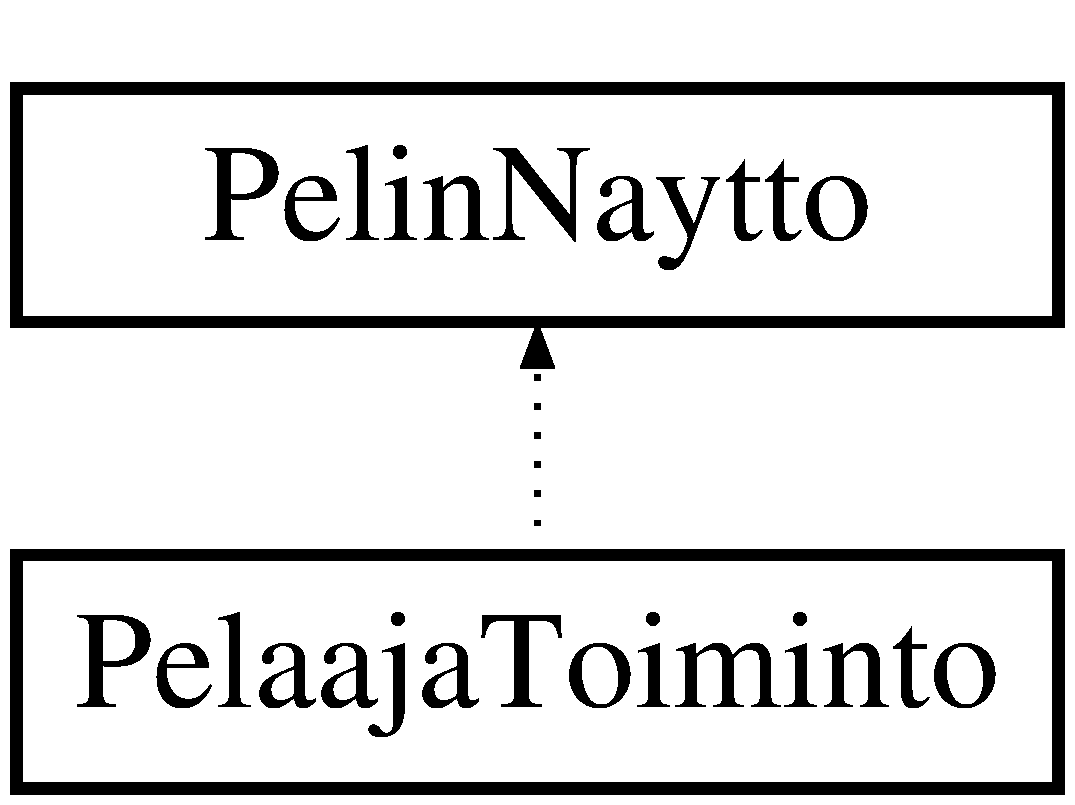
\includegraphics[height=2.000000cm]{class_pelaaja_toiminto}
\end{center}
\end{figure}
\subsection*{Public Member Functions}
\begin{DoxyCompactItemize}
\item 
\hyperlink{class_pelaaja_toiminto_af435c652c81b413af351e84e98ca4027}{Pelaaja\+Toiminto} (\hyperlink{class_julkinen_1_1_nayttorajapinta}{Julkinen\+::\+Nayttorajapinta} $\ast$naytto, \hyperlink{class_julkinen_1_1_koordinaatti}{Julkinen\+::\+Koordinaatti} const \&koko, \hyperlink{class_data}{Data} $\ast$data)
\begin{DoxyCompactList}\small\item\em \hyperlink{class_pelaaja_toiminto}{Pelaaja\+Toiminto} luokan rakentaja. \end{DoxyCompactList}\item 
\hyperlink{class_pelaaja_toiminto_a8a27af3770a1fbf0148a75ed51fe3f0e}{$\sim$\+Pelaaja\+Toiminto} ()
\begin{DoxyCompactList}\small\item\em Purkaja. \end{DoxyCompactList}\item 
void \hyperlink{class_pelaaja_toiminto_aa9015f6a8af946a3139eaed1de6555f3}{aseta\+Koko} (\hyperlink{class_julkinen_1_1_koordinaatti}{Julkinen\+::\+Koordinaatti} const \&koko)
\begin{DoxyCompactList}\small\item\em Koon asettaja. \end{DoxyCompactList}\item 
bool \hyperlink{class_pelaaja_toiminto_a59e41355414eabee8fbbb8ebfbe94d64}{Tyonna} (\hyperlink{namespace_julkinen_acce0eefc4c90f907dd5fb319b0d05872}{Julkinen\+::\+Reuna} reuna, unsigned int paikka, unsigned int rotaatio, \hyperlink{class_pelaaja}{Pelaaja} $\ast$pelaaja)
\begin{DoxyCompactList}\small\item\em Pelaajan liikuttaja. \end{DoxyCompactList}\item 
bool \hyperlink{class_pelaaja_toiminto_afd40ede2b643b2e51bb101b1790903b2}{Liiku} (\hyperlink{namespace_julkinen_a81b50e3c6f21c0c1c46e186592107c3c}{Julkinen\+::\+Suunta} suunta, unsigned int maara, \hyperlink{class_pelaaja}{Pelaaja} $\ast$pelaaja)
\begin{DoxyCompactList}\small\item\em Pelaajan liikuttaja. \end{DoxyCompactList}\end{DoxyCompactItemize}


\subsection{Detailed Description}
Labyrintti-\/pelin pelaajan toimintojen suoritus luokka. 

\subsection{Constructor \& Destructor Documentation}
\hypertarget{class_pelaaja_toiminto_af435c652c81b413af351e84e98ca4027}{}\index{Pelaaja\+Toiminto@{Pelaaja\+Toiminto}!Pelaaja\+Toiminto@{Pelaaja\+Toiminto}}
\index{Pelaaja\+Toiminto@{Pelaaja\+Toiminto}!Pelaaja\+Toiminto@{Pelaaja\+Toiminto}}
\subsubsection[{Pelaaja\+Toiminto(\+Julkinen\+::\+Nayttorajapinta $\ast$naytto, Julkinen\+::\+Koordinaatti const \&koko, Data $\ast$data)}]{\setlength{\rightskip}{0pt plus 5cm}Pelaaja\+Toiminto\+::\+Pelaaja\+Toiminto (
\begin{DoxyParamCaption}
\item[{{\bf Julkinen\+::\+Nayttorajapinta} $\ast$}]{naytto, }
\item[{{\bf Julkinen\+::\+Koordinaatti} const \&}]{koko, }
\item[{{\bf Data} $\ast$}]{data}
\end{DoxyParamCaption}
)}\label{class_pelaaja_toiminto_af435c652c81b413af351e84e98ca4027}


\hyperlink{class_pelaaja_toiminto}{Pelaaja\+Toiminto} luokan rakentaja. 

\begin{DoxyPrecond}{Precondition}
Annettu naytto ja data ovat oikeita osoitteita.
\end{DoxyPrecond}
Asettaa käytettävän näytön, koon ja datan.


\begin{DoxyParams}[1]{Parameters}
\mbox{\tt in}  & {\em naytto} & Käytettävä näyttö {\ttfamily \hyperlink{class_julkinen_1_1_nayttorajapinta}{Julkinen\+::\+Nayttorajapinta}}-\/luokkan osoitteena. \\
\hline
\mbox{\tt in}  & {\em koko} & Näytön koko {\ttfamily \hyperlink{class_julkinen_1_1_koordinaatti}{Julkinen\+::\+Koordinaatti}}-\/luokkana. \\
\hline
\mbox{\tt in}  & {\em data} & Käytettävä data {\ttfamily \hyperlink{class_data}{Data}}-\/luokkan osoitteena. \\
\hline
\end{DoxyParams}
\hypertarget{class_pelaaja_toiminto_a8a27af3770a1fbf0148a75ed51fe3f0e}{}\index{Pelaaja\+Toiminto@{Pelaaja\+Toiminto}!````~Pelaaja\+Toiminto@{$\sim$\+Pelaaja\+Toiminto}}
\index{````~Pelaaja\+Toiminto@{$\sim$\+Pelaaja\+Toiminto}!Pelaaja\+Toiminto@{Pelaaja\+Toiminto}}
\subsubsection[{$\sim$\+Pelaaja\+Toiminto()}]{\setlength{\rightskip}{0pt plus 5cm}Pelaaja\+Toiminto\+::$\sim$\+Pelaaja\+Toiminto (
\begin{DoxyParamCaption}
{}
\end{DoxyParamCaption}
)}\label{class_pelaaja_toiminto_a8a27af3770a1fbf0148a75ed51fe3f0e}


Purkaja. 

\begin{DoxyPostcond}{Postcondition}
No-\/throw takuu. 
\end{DoxyPostcond}


\subsection{Member Function Documentation}
\hypertarget{class_pelaaja_toiminto_aa9015f6a8af946a3139eaed1de6555f3}{}\index{Pelaaja\+Toiminto@{Pelaaja\+Toiminto}!aseta\+Koko@{aseta\+Koko}}
\index{aseta\+Koko@{aseta\+Koko}!Pelaaja\+Toiminto@{Pelaaja\+Toiminto}}
\subsubsection[{aseta\+Koko(\+Julkinen\+::\+Koordinaatti const \&koko)}]{\setlength{\rightskip}{0pt plus 5cm}void Pelaaja\+Toiminto\+::aseta\+Koko (
\begin{DoxyParamCaption}
\item[{{\bf Julkinen\+::\+Koordinaatti} const \&}]{koko}
\end{DoxyParamCaption}
)}\label{class_pelaaja_toiminto_aa9015f6a8af946a3139eaed1de6555f3}


Koon asettaja. 

Asettaa yksityisen kentän kokoa säilyttävän {\ttfamily \hyperlink{class_julkinen_1_1_koordinaatti}{Julkinen\+::\+Koordinaatti}} luokan \+\_\+koko


\begin{DoxyParams}[1]{Parameters}
\mbox{\tt in}  & {\em koko} & Pelialueen koko {\ttfamily \hyperlink{class_julkinen_1_1_koordinaatti}{Julkinen\+::\+Koordinaatti}}-\/luokkana. \\
\hline
\end{DoxyParams}
\hypertarget{class_pelaaja_toiminto_afd40ede2b643b2e51bb101b1790903b2}{}\index{Pelaaja\+Toiminto@{Pelaaja\+Toiminto}!Liiku@{Liiku}}
\index{Liiku@{Liiku}!Pelaaja\+Toiminto@{Pelaaja\+Toiminto}}
\subsubsection[{Liiku(\+Julkinen\+::\+Suunta suunta, unsigned int maara, Pelaaja $\ast$pelaaja)}]{\setlength{\rightskip}{0pt plus 5cm}bool Pelaaja\+Toiminto\+::\+Liiku (
\begin{DoxyParamCaption}
\item[{{\bf Julkinen\+::\+Suunta}}]{suunta, }
\item[{unsigned int}]{maara, }
\item[{{\bf Pelaaja} $\ast$}]{pelaaja}
\end{DoxyParamCaption}
)}\label{class_pelaaja_toiminto_afd40ede2b643b2e51bb101b1790903b2}


Pelaajan liikuttaja. 

\begin{DoxyPrecond}{Precondition}
Osoite {\ttfamily \hyperlink{class_pelaaja}{Pelaaja}}-\/luokaan on oikea.
\end{DoxyPrecond}
Hoitaa pelaajan työntö käskyn suorituksen. Tätä kutsutaan {\ttfamily \hyperlink{class_peli}{Peli}} luokassa, kun {\ttfamily \hyperlink{class_komentotulkki}{Komentotulkki}} luokka antaa työntö komennon


\begin{DoxyParams}[1]{Parameters}
\mbox{\tt in}  & {\em reuna} & Laudan työntö reuna {\ttfamily \hyperlink{namespace_julkinen_acce0eefc4c90f907dd5fb319b0d05872}{Julkinen\+::\+Reuna}}-\/luokkana. \\
\hline
\mbox{\tt in}  & {\em paikka} & {\ttfamily Työnnön} paikka reunalta. \\
\hline
\mbox{\tt in}  & {\em rotaatio} & {\ttfamily Työnnettävän} palan rotaatio. \\
\hline
\mbox{\tt in}  & {\em pelaaja} & Työntävä pelaaja {\ttfamily \hyperlink{class_pelaaja}{Pelaaja}}-\/luokan osoitteena.\\
\hline
\end{DoxyParams}

\begin{DoxyExceptions}{Exceptions}
{\em Toimintovirhe} & pelaaja ei ole työntänyt irtopalaa vuorollansa. \\
\hline
{\em Toimintovirhe} & pelaaja on jo liikkunut vuorollansa. \\
\hline
{\em Toimintovirhe} & liikkeen suunta on virheellinen. \\
\hline
{\em Toimintovirhe} & pelaaja ei voi liikkua annettua määrää.\\
\hline
\end{DoxyExceptions}
\begin{DoxyPostcond}{Postcondition}
Tieto siitä onnistuko liikkuminen 
\end{DoxyPostcond}
\hypertarget{class_pelaaja_toiminto_a59e41355414eabee8fbbb8ebfbe94d64}{}\index{Pelaaja\+Toiminto@{Pelaaja\+Toiminto}!Tyonna@{Tyonna}}
\index{Tyonna@{Tyonna}!Pelaaja\+Toiminto@{Pelaaja\+Toiminto}}
\subsubsection[{Tyonna(\+Julkinen\+::\+Reuna reuna, unsigned int paikka, unsigned int rotaatio, Pelaaja $\ast$pelaaja)}]{\setlength{\rightskip}{0pt plus 5cm}bool Pelaaja\+Toiminto\+::\+Tyonna (
\begin{DoxyParamCaption}
\item[{{\bf Julkinen\+::\+Reuna}}]{reuna, }
\item[{unsigned int}]{paikka, }
\item[{unsigned int}]{rotaatio, }
\item[{{\bf Pelaaja} $\ast$}]{pelaaja}
\end{DoxyParamCaption}
)}\label{class_pelaaja_toiminto_a59e41355414eabee8fbbb8ebfbe94d64}


Pelaajan liikuttaja. 

\begin{DoxyPrecond}{Precondition}
Osoite {\ttfamily \hyperlink{class_pelaaja}{Pelaaja}}-\/luokaan on oikea.
\end{DoxyPrecond}
Hoitaa pelaajan liikuttamisen. Tätä kutsutaan {\ttfamily \hyperlink{class_peli}{Peli}} luokassa, kun {\ttfamily \hyperlink{class_komentotulkki}{Komentotulkki}} luokka antaa liikkumis komennon tai oma {\ttfamily suorita\+Automaatti\+Liike} metodi suorittaa liikeen.


\begin{DoxyParams}[1]{Parameters}
\mbox{\tt in}  & {\em suunta} & Liikkeen suunta {\ttfamily \hyperlink{namespace_julkinen_a81b50e3c6f21c0c1c46e186592107c3c}{Julkinen\+::\+Suunta}}-\/luokkana. \\
\hline
\mbox{\tt in}  & {\em maara} & {\ttfamily Liikkeen} määrä. \\
\hline
\mbox{\tt in}  & {\em pelaaja} & Liikutettava pelaaja {\ttfamily \hyperlink{class_pelaaja}{Pelaaja}}-\/luokan osoitteena.\\
\hline
\end{DoxyParams}

\begin{DoxyExceptions}{Exceptions}
{\em Toimintovirhe} & irtopalan reuna on virheellinen. \\
\hline
{\em Toimintovirhe} & irtopalan paikka on virheellinen. \\
\hline
{\em Toimintovirhe} & irtopalan rotaatio on virheellinen. \\
\hline
{\em Toimintovirhe} & pelaaja on jo työntänyt vuorollansa.\\
\hline
\end{DoxyExceptions}
\begin{DoxyPostcond}{Postcondition}
Tieto siitä onnistuko työntö 
\end{DoxyPostcond}


The documentation for this class was generated from the following files\+:\begin{DoxyCompactItemize}
\item 
\hyperlink{_pelaaja_toiminto_8hpp}{Pelaaja\+Toiminto.\+hpp}\item 
Pelaaja\+Toiminto.\+cpp\end{DoxyCompactItemize}

\hypertarget{class_peli}{}\section{Peli Class Reference}
\label{class_peli}\index{Peli@{Peli}}


Labyrintti-\/pelin pelin toimintojen suorittava luokka.  




{\ttfamily \#include $<$Peli.\+hpp$>$}

Inheritance diagram for Peli\+:\begin{figure}[H]
\begin{center}
\leavevmode
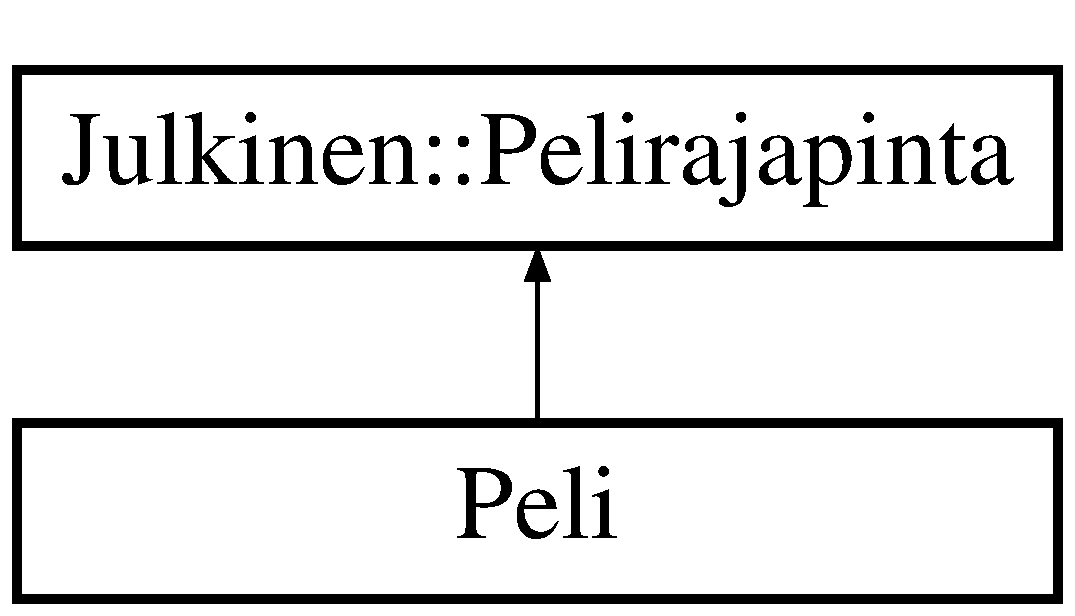
\includegraphics[height=2.000000cm]{class_peli}
\end{center}
\end{figure}
\subsection*{Public Member Functions}
\begin{DoxyCompactItemize}
\item 
virtual bool \hyperlink{class_peli_a468618c1872582a68f85a5ef34defc19}{onko\+Alustustilassa} () const 
\begin{DoxyCompactList}\small\item\em Kertoo onko peli alustustilassa. \end{DoxyCompactList}\item 
virtual void \hyperlink{class_peli_a3fabca61c1c2707cb3810043bffa71c2}{lisaa\+Naytto} (\hyperlink{class_julkinen_1_1_nayttorajapinta}{Julkinen\+::\+Nayttorajapinta} $\ast$naytto)
\begin{DoxyCompactList}\small\item\em Lisaa tulostus olion peliin. \end{DoxyCompactList}\item 
virtual void \hyperlink{class_peli_adc8656a5e41df3c1343b2fa21495fbff}{maarita\+Pelialueen\+Koko} (\hyperlink{class_julkinen_1_1_koordinaatti}{Julkinen\+::\+Koordinaatti} const \&koko)
\begin{DoxyCompactList}\small\item\em Maarittaa pelikentän koon. \end{DoxyCompactList}\item 
virtual void \hyperlink{class_peli_a5061cb0a10052090128302e1619d1188}{lisaa\+Pelaaja} (\hyperlink{namespace_julkinen_ad9a0a9e01af78249f584a93b03db4329}{Julkinen\+::\+Pelaaja\+Tyyppi} tyyppi, std\+::string const \&nimi, char lyhenne, \hyperlink{class_julkinen_1_1_koordinaatti}{Julkinen\+::\+Koordinaatti} const \&sijainti)
\begin{DoxyCompactList}\small\item\em Pelin alustusfunktio, joka lisaa pelaajan peliin. \end{DoxyCompactList}\item 
virtual void \hyperlink{class_peli_a2d53bbe19ae97fe59ae37c05c72f4e51}{lisaa\+Pala} (\hyperlink{namespace_julkinen_a272c70e0503191a485c8a9cd4281e6f5}{Julkinen\+::\+Pala\+Tyyppi} pala, unsigned int rotaatio, \hyperlink{class_julkinen_1_1_koordinaatti}{Julkinen\+::\+Koordinaatti} const \&sijainti)
\begin{DoxyCompactList}\small\item\em Pelin alustusfunktio, joka lisaa palan peliin. \end{DoxyCompactList}\item 
virtual void \hyperlink{class_peli_a81f3587c603c96ddd127527f3772b19f}{lisaa\+Esine} (char merkki, \hyperlink{class_julkinen_1_1_koordinaatti}{Julkinen\+::\+Koordinaatti} const \&sijainti, std\+::string const \&pelaaja)
\begin{DoxyCompactList}\small\item\em Pelin alustusfunktio, joka lisaa esineen peliin. \end{DoxyCompactList}\item 
virtual void \hyperlink{class_peli_a8045f08b5aa05114baced0541142e735}{aseta\+Palan\+Tyyppi} (\hyperlink{namespace_julkinen_afc26052e09d0b2214f749492cc5fff19}{Julkinen\+::\+Erikoispala\+Tyyppi} tyyppi, \hyperlink{class_julkinen_1_1_koordinaatti}{Julkinen\+::\+Koordinaatti} const \&sijainti, \hyperlink{class_julkinen_1_1_koordinaatti}{Julkinen\+::\+Koordinaatti} const \&kohde=\hyperlink{class_julkinen_1_1_koordinaatti}{Julkinen\+::\+Koordinaatti}())
\begin{DoxyCompactList}\small\item\em Pelin alustusfunktio, joka asettaa palan erikoispalan tyypin. \end{DoxyCompactList}\item 
virtual void \hyperlink{class_peli_a65eff799de42881efc08f7994b27968e}{alustus\+Lopeta} ()
\begin{DoxyCompactList}\small\item\em Lopettaa pelin alustuksen. \end{DoxyCompactList}\item 
virtual bool \hyperlink{class_peli_a05f3cde8cc44cad1e083312d208721f3}{onko\+Pelitilassa} () const 
\begin{DoxyCompactList}\small\item\em Kertoo onko peli pelitilassa. \end{DoxyCompactList}\item 
virtual void \hyperlink{class_peli_a4093d9ae2c4b220a4da9bcc728f7d59b}{komento\+Tyonna} (\hyperlink{namespace_julkinen_acce0eefc4c90f907dd5fb319b0d05872}{Julkinen\+::\+Reuna} reuna, unsigned int paikka, unsigned int rotaatio)
\begin{DoxyCompactList}\small\item\em Työntää irtopalan annettuun kohtaan. \end{DoxyCompactList}\item 
virtual void \hyperlink{class_peli_ad721f34f1e12e0dae3e2f73de2d99d05}{komento\+Liiku} (\hyperlink{namespace_julkinen_a81b50e3c6f21c0c1c46e186592107c3c}{Julkinen\+::\+Suunta} suunta, unsigned int maara=0)
\begin{DoxyCompactList}\small\item\em Liikuttaa vuorossa olevaa pelaajaa. \end{DoxyCompactList}\item 
virtual bool \hyperlink{class_peli_a6788584913d8417dd2fa0bf486e5a3b3}{vaihda\+Vuoro} ()
\begin{DoxyCompactList}\small\item\em Vaihtaa vuoron seuraavalle pelaajalle ja ilmoittaa, jatketaanko peliä, vai onko jokin pelaaja voittanut pelin. {\bfseries Huom!} Raakilepalautuksessa tulkitaan, että kukaan ei voita peliä koskaan (koska kerättäviä esineitä ei ole). \end{DoxyCompactList}\item 
virtual \hyperlink{namespace_julkinen_ad9a0a9e01af78249f584a93b03db4329}{Julkinen\+::\+Pelaaja\+Tyyppi} \hyperlink{class_peli_a43524af1c4c914acc5faf872b5dcf890}{hae\+Vuorossa} ()
\begin{DoxyCompactList}\small\item\em Palauttaa vuorossa olevan pelaajan tyypin. \end{DoxyCompactList}\end{DoxyCompactItemize}


\subsection{Detailed Description}
Labyrintti-\/pelin pelin toimintojen suorittava luokka. 

\subsection{Member Function Documentation}
\hypertarget{class_peli_a65eff799de42881efc08f7994b27968e}{}\index{Peli@{Peli}!alustus\+Lopeta@{alustus\+Lopeta}}
\index{alustus\+Lopeta@{alustus\+Lopeta}!Peli@{Peli}}
\subsubsection[{alustus\+Lopeta()}]{\setlength{\rightskip}{0pt plus 5cm}void Peli\+::alustus\+Lopeta (
\begin{DoxyParamCaption}
{}
\end{DoxyParamCaption}
)\hspace{0.3cm}{\ttfamily [virtual]}}\label{class_peli_a65eff799de42881efc08f7994b27968e}


Lopettaa pelin alustuksen. 

\begin{DoxyPrecond}{Precondition}
\hyperlink{class_peli}{Peli} on alustettu. 
\end{DoxyPrecond}
\begin{DoxyPostcond}{Postcondition}
\hyperlink{class_peli}{Peli} on pelitilassa. Poikkeustakuu\+: Perustakuu poikkeuksen sattuessa. 
\end{DoxyPostcond}


Implements \hyperlink{class_julkinen_1_1_pelirajapinta_afdcc11ea245937075026e82be6e9a874}{Julkinen\+::\+Pelirajapinta}.

\hypertarget{class_peli_a8045f08b5aa05114baced0541142e735}{}\index{Peli@{Peli}!aseta\+Palan\+Tyyppi@{aseta\+Palan\+Tyyppi}}
\index{aseta\+Palan\+Tyyppi@{aseta\+Palan\+Tyyppi}!Peli@{Peli}}
\subsubsection[{aseta\+Palan\+Tyyppi(\+Julkinen\+::\+Erikoispala\+Tyyppi tyyppi, Julkinen\+::\+Koordinaatti const \&sijainti, Julkinen\+::\+Koordinaatti const \&kohde=\+Julkinen\+::\+Koordinaatti())}]{\setlength{\rightskip}{0pt plus 5cm}void Peli\+::aseta\+Palan\+Tyyppi (
\begin{DoxyParamCaption}
\item[{{\bf Julkinen\+::\+Erikoispala\+Tyyppi}}]{tyyppi, }
\item[{{\bf Julkinen\+::\+Koordinaatti} const \&}]{sijainti, }
\item[{{\bf Julkinen\+::\+Koordinaatti} const \&}]{kohde = {\ttfamily {\bf Julkinen\+::\+Koordinaatti}()}}
\end{DoxyParamCaption}
)\hspace{0.3cm}{\ttfamily [virtual]}}\label{class_peli_a8045f08b5aa05114baced0541142e735}


Pelin alustusfunktio, joka asettaa palan erikoispalan tyypin. 

\begin{DoxyPrecond}{Precondition}
\hyperlink{class_peli}{Peli} on alustustilassa. Pelilauta ja palat on alustettu. 
\end{DoxyPrecond}
\begin{DoxyPostcond}{Postcondition}
Palan erikoisominaisuudet on luotu. Poikkeustakuu\+: Perustakuu poikkeuksen sattuessa.
\end{DoxyPostcond}

\begin{DoxyParams}[1]{Parameters}
\mbox{\tt in}  & {\em tyyppi} & Palan erikoistyyppi, joka kertoo onko pala normaali, teleportti, siunattu tai kirottu. \\
\hline
\mbox{\tt in}  & {\em sijainti} & Kertoo mitä labyrintin palaa käsitellään. \\
\hline
\mbox{\tt in}  & {\em kohde} & Teleportti-\/palan kohderuudun koordinaatti, muilla paloilla parametria ei anneta.\\
\hline
\end{DoxyParams}

\begin{DoxyExceptions}{Exceptions}
{\em Alustusvirhe} & Annettu koordinaatti on pelialueen ulkopuolella. \\
\hline
\end{DoxyExceptions}


Implements \hyperlink{class_julkinen_1_1_pelirajapinta_a4de5389102fb5a479173cc3728b989dd}{Julkinen\+::\+Pelirajapinta}.

\hypertarget{class_peli_a43524af1c4c914acc5faf872b5dcf890}{}\index{Peli@{Peli}!hae\+Vuorossa@{hae\+Vuorossa}}
\index{hae\+Vuorossa@{hae\+Vuorossa}!Peli@{Peli}}
\subsubsection[{hae\+Vuorossa()}]{\setlength{\rightskip}{0pt plus 5cm}{\bf Julkinen\+::\+Pelaaja\+Tyyppi} Peli\+::hae\+Vuorossa (
\begin{DoxyParamCaption}
{}
\end{DoxyParamCaption}
)\hspace{0.3cm}{\ttfamily [virtual]}}\label{class_peli_a43524af1c4c914acc5faf872b5dcf890}


Palauttaa vuorossa olevan pelaajan tyypin. 

\begin{DoxyPrecond}{Precondition}
\hyperlink{class_peli}{Peli} on pelitilassa. 
\end{DoxyPrecond}
\begin{DoxyPostcond}{Postcondition}
\hyperlink{class_peli}{Peli} on pelitilassa ja vuorossa olevan pelaajan {\ttfamily Pelaaja\+Tyyppi} on palautettu. Poikkeustakuu\+: No-\/throw takuu.
\end{DoxyPostcond}
\begin{DoxyReturn}{Returns}
Palauttaa vuorossa olevan pelaajan {\ttfamily Pelaaja\+Tyyppi}. 
\end{DoxyReturn}


Implements \hyperlink{class_julkinen_1_1_pelirajapinta_aef0e254fd13ac8a44bb9db0908daa0e7}{Julkinen\+::\+Pelirajapinta}.

\hypertarget{class_peli_ad721f34f1e12e0dae3e2f73de2d99d05}{}\index{Peli@{Peli}!komento\+Liiku@{komento\+Liiku}}
\index{komento\+Liiku@{komento\+Liiku}!Peli@{Peli}}
\subsubsection[{komento\+Liiku(\+Julkinen\+::\+Suunta suunta, unsigned int maara=0)}]{\setlength{\rightskip}{0pt plus 5cm}void Peli\+::komento\+Liiku (
\begin{DoxyParamCaption}
\item[{{\bf Julkinen\+::\+Suunta}}]{suunta, }
\item[{unsigned int}]{maara = {\ttfamily 0}}
\end{DoxyParamCaption}
)\hspace{0.3cm}{\ttfamily [virtual]}}\label{class_peli_ad721f34f1e12e0dae3e2f73de2d99d05}


Liikuttaa vuorossa olevaa pelaajaa. 

Liikuttaa vuorossa olevaa pelaajaa annettuun suuntaan annetun määrän. Jos pelaaja ei pysty liikkumaan annettuun suuntaan annettua määrää heitetään Toimintovirhe. Toimintovirhe heitetään myös silloin jos pelaaja ei ole työntänyt palaa tällä vuorolla, paitsi jos suunta on A\+U\+T\+O\+M\+A\+A\+T\+T\+I. Raakilepalautuksessa liikkuminen suoritetaan, vaikka työntämistä ei olekaan suoritettu (eli poikkeusta ei heitetä).

\begin{DoxyPrecond}{Precondition}
\hyperlink{class_peli}{Peli} on pelitilassa. 
\end{DoxyPrecond}
\begin{DoxyPostcond}{Postcondition}
\hyperlink{class_pelaaja}{Pelaaja} on liikutettu ja pelilauta on tulostettu uudestaan. Poikkeustakuu\+: Vahvatakuu Komentovirhe tai Toimintovirhe poikkeuksen sattuessa.
\end{DoxyPostcond}

\begin{DoxyParams}[1]{Parameters}
\mbox{\tt in}  & {\em suunta} & Suunta johon pelaajaa siirretään. \\
\hline
\mbox{\tt in}  & {\em maara} & Pelaajan liikkumien ruutujen määrä.\\
\hline
\end{DoxyParams}

\begin{DoxyExceptions}{Exceptions}
{\em Toimintovirhe} & Vuorossa oleva pelaaja ei voi liikkua annettuun suuntaan annettua määrää. \\
\hline
{\em Toimintovirhe} & Vuorossa oleva pelaaja ei ole työntänyt irtopalaa. Ei heitetä jos suunta on A\+U\+T\+O\+M\+A\+A\+T\+T\+I. Ei heitetä raakilepalautuksessa. \\
\hline
{\em Komentovirhe} & maara on negatiivinen. \\
\hline
{\em Komentovirhe} & maara on 0, mutta suunta ei ole P\+A\+I\+K\+A\+L\+L\+A\+A\+N. \\
\hline
\end{DoxyExceptions}


Implements \hyperlink{class_julkinen_1_1_pelirajapinta_a3444c155143baff73521a0707712b36a}{Julkinen\+::\+Pelirajapinta}.

\hypertarget{class_peli_a4093d9ae2c4b220a4da9bcc728f7d59b}{}\index{Peli@{Peli}!komento\+Tyonna@{komento\+Tyonna}}
\index{komento\+Tyonna@{komento\+Tyonna}!Peli@{Peli}}
\subsubsection[{komento\+Tyonna(\+Julkinen\+::\+Reuna reuna, unsigned int paikka, unsigned int rotaatio)}]{\setlength{\rightskip}{0pt plus 5cm}void Peli\+::komento\+Tyonna (
\begin{DoxyParamCaption}
\item[{{\bf Julkinen\+::\+Reuna}}]{reuna, }
\item[{unsigned int}]{paikka, }
\item[{unsigned int}]{rotaatio}
\end{DoxyParamCaption}
)\hspace{0.3cm}{\ttfamily [virtual]}}\label{class_peli_a4093d9ae2c4b220a4da9bcc728f7d59b}


Työntää irtopalan annettuun kohtaan. 

Raakilepalautuksessa tätä operaatiota ei kutsuta.

\begin{DoxyPrecond}{Precondition}
\hyperlink{class_peli}{Peli} on pelitilassa. 
\end{DoxyPrecond}
\begin{DoxyPostcond}{Postcondition}
Irtopala on asetettu annettuun kohtaan ja työntö kohdan työntösuunnan mukaisen vastapään pala on otettu uudeksi irtopalaksi. Pelilauta on tulostettu uudestaan. Poikkeustakuu\+: Vahvatakuu Komentovirhe poikkeuksen sattuessa.
\end{DoxyPostcond}

\begin{DoxyParams}[1]{Parameters}
\mbox{\tt in}  & {\em reuna} & Reuna jolle pala työnnetään. \\
\hline
\mbox{\tt in}  & {\em rotaatio} & Työnnettävän palan rotaatio (1-\/4) \\
\hline
\mbox{\tt in}  & {\em paikka} & Mihin kohtaan reunaa pala työnnetään.\\
\hline
\end{DoxyParams}

\begin{DoxyExceptions}{Exceptions}
{\em Toimintovirhe} & \hyperlink{class_pelaaja}{Pelaaja} on jo työntänyt palaa tällä vuorolla. \\
\hline
{\em Komentovirhe} & Paikka on virheellinen. \\
\hline
{\em Komentovirhe} & Rotaatio on virheellinen. \\
\hline
\end{DoxyExceptions}


Implements \hyperlink{class_julkinen_1_1_pelirajapinta_aea8cbb43bcf85664b97d17df1666ce9f}{Julkinen\+::\+Pelirajapinta}.

\hypertarget{class_peli_a81f3587c603c96ddd127527f3772b19f}{}\index{Peli@{Peli}!lisaa\+Esine@{lisaa\+Esine}}
\index{lisaa\+Esine@{lisaa\+Esine}!Peli@{Peli}}
\subsubsection[{lisaa\+Esine(char merkki, Julkinen\+::\+Koordinaatti const \&sijainti, std\+::string const \&pelaaja)}]{\setlength{\rightskip}{0pt plus 5cm}void Peli\+::lisaa\+Esine (
\begin{DoxyParamCaption}
\item[{char}]{merkki, }
\item[{{\bf Julkinen\+::\+Koordinaatti} const \&}]{sijainti, }
\item[{std\+::string const \&}]{pelaaja}
\end{DoxyParamCaption}
)\hspace{0.3cm}{\ttfamily [virtual]}}\label{class_peli_a81f3587c603c96ddd127527f3772b19f}


Pelin alustusfunktio, joka lisaa esineen peliin. 

\begin{DoxyPrecond}{Precondition}
\hyperlink{class_peli}{Peli} on alustustilassa. Pelilauta ja pelaajat on alustettu. 
\end{DoxyPrecond}
\begin{DoxyPostcond}{Postcondition}
\hyperlink{class_esine}{Esine} on lisatty peliin ja mahdollisesti annetulle pelaajalle, esine on lisätty kerättäviin esineisiin. Poikkeustakuu\+: Perustakuu poikkeuksen sattuessa.
\end{DoxyPostcond}

\begin{DoxyParams}[1]{Parameters}
\mbox{\tt in}  & {\em merkki} & Esinettä kuvaava merkki pelissä. \\
\hline
\mbox{\tt in}  & {\em sijainti} & Kertoo mihin labyrintin koordinaattiin esine laitetaan. \\
\hline
\mbox{\tt in}  & {\em pelaaja} & Pelaajan nimi jonka tehtävänä on poimia esine.\\
\hline
\end{DoxyParams}

\begin{DoxyExceptions}{Exceptions}
{\em Alustusvirhe} & Pelaajaa ei ole lisatty peliin. \\
\hline
{\em Alustusvirhe} & Annettu koordinaatti on pelialueen ulkopuolella. \\
\hline
\end{DoxyExceptions}


Implements \hyperlink{class_julkinen_1_1_pelirajapinta_a998c0b644b8b1b73ac74390afea03da9}{Julkinen\+::\+Pelirajapinta}.

\hypertarget{class_peli_a3fabca61c1c2707cb3810043bffa71c2}{}\index{Peli@{Peli}!lisaa\+Naytto@{lisaa\+Naytto}}
\index{lisaa\+Naytto@{lisaa\+Naytto}!Peli@{Peli}}
\subsubsection[{lisaa\+Naytto(\+Julkinen\+::\+Nayttorajapinta $\ast$naytto)}]{\setlength{\rightskip}{0pt plus 5cm}void Peli\+::lisaa\+Naytto (
\begin{DoxyParamCaption}
\item[{{\bf Julkinen\+::\+Nayttorajapinta} $\ast$}]{naytto}
\end{DoxyParamCaption}
)\hspace{0.3cm}{\ttfamily [virtual]}}\label{class_peli_a3fabca61c1c2707cb3810043bffa71c2}


Lisaa tulostus olion peliin. 

\begin{DoxyPrecond}{Precondition}
\hyperlink{class_peli}{Peli} on alustustilassa. Annettu parametri ei ole tyhjä. Näyttöä ei ole lisätty. 
\end{DoxyPrecond}
\begin{DoxyPostcond}{Postcondition}
Tulostus-\/olio lisätty peliin. Poikkeustakuu\+: No-\/throw takuu.
\end{DoxyPostcond}

\begin{DoxyParams}[1]{Parameters}
\mbox{\tt in,out}  & {\em naytto} & osoitin Nayttorajapinta -\/luokan toteuttavaan olioon. \\
\hline
\end{DoxyParams}


Implements \hyperlink{class_julkinen_1_1_pelirajapinta_ad1597bf68505144431c62cc7c6e49bf6}{Julkinen\+::\+Pelirajapinta}.

\hypertarget{class_peli_a2d53bbe19ae97fe59ae37c05c72f4e51}{}\index{Peli@{Peli}!lisaa\+Pala@{lisaa\+Pala}}
\index{lisaa\+Pala@{lisaa\+Pala}!Peli@{Peli}}
\subsubsection[{lisaa\+Pala(\+Julkinen\+::\+Pala\+Tyyppi pala, unsigned int rotaatio, Julkinen\+::\+Koordinaatti const \&sijainti)}]{\setlength{\rightskip}{0pt plus 5cm}void Peli\+::lisaa\+Pala (
\begin{DoxyParamCaption}
\item[{{\bf Julkinen\+::\+Pala\+Tyyppi}}]{pala, }
\item[{unsigned int}]{rotaatio, }
\item[{{\bf Julkinen\+::\+Koordinaatti} const \&}]{sijainti}
\end{DoxyParamCaption}
)\hspace{0.3cm}{\ttfamily [virtual]}}\label{class_peli_a2d53bbe19ae97fe59ae37c05c72f4e51}


Pelin alustusfunktio, joka lisaa palan peliin. 

\begin{DoxyPrecond}{Precondition}
\hyperlink{class_peli}{Peli} on alustustilassa. Pelialueen koko on määritelty. Annettuun koordinaattiin ei vielä lisätty palaa. 
\end{DoxyPrecond}
\begin{DoxyPostcond}{Postcondition}
Pelilautaan on lisätty pala. Poikkeustakuu\+: Perustakuu poikkeuksen sattuessa.
\end{DoxyPostcond}

\begin{DoxyParams}[1]{Parameters}
\mbox{\tt in}  & {\em pala} & Tieto siitä minkä laista palaa lisätään. \\
\hline
\mbox{\tt in}  & {\em rotaatio} & Lisättävän palan rotaatio (1-\/4). rotaatiota ei tarkasteta jos irtopala \\
\hline
\mbox{\tt in}  & {\em sijainti} & koordinaatti mihin pala lisätään. Jos sijainti.\+onko\+Irtopala() palautaa {\ttfamily true}, niin lisättävä pala on irtopala.\\
\hline
\end{DoxyParams}

\begin{DoxyExceptions}{Exceptions}
{\em Alustusvirhe} & Annettu koordinaatti on pelialueen ulkopuolella. \\
\hline
{\em Alustusvirhe} & Annettu rotaatio on virheellinen. \\
\hline
\end{DoxyExceptions}


Implements \hyperlink{class_julkinen_1_1_pelirajapinta_a149820998333ec4d7fa9fd3ff5ea98fd}{Julkinen\+::\+Pelirajapinta}.

\hypertarget{class_peli_a5061cb0a10052090128302e1619d1188}{}\index{Peli@{Peli}!lisaa\+Pelaaja@{lisaa\+Pelaaja}}
\index{lisaa\+Pelaaja@{lisaa\+Pelaaja}!Peli@{Peli}}
\subsubsection[{lisaa\+Pelaaja(\+Julkinen\+::\+Pelaaja\+Tyyppi tyyppi, std\+::string const \&nimi, char lyhenne, Julkinen\+::\+Koordinaatti const \&sijainti)}]{\setlength{\rightskip}{0pt plus 5cm}void Peli\+::lisaa\+Pelaaja (
\begin{DoxyParamCaption}
\item[{{\bf Julkinen\+::\+Pelaaja\+Tyyppi}}]{tyyppi, }
\item[{std\+::string const \&}]{nimi, }
\item[{char}]{lyhenne, }
\item[{{\bf Julkinen\+::\+Koordinaatti} const \&}]{sijainti}
\end{DoxyParamCaption}
)\hspace{0.3cm}{\ttfamily [virtual]}}\label{class_peli_a5061cb0a10052090128302e1619d1188}


Pelin alustusfunktio, joka lisaa pelaajan peliin. 

\begin{DoxyPrecond}{Precondition}
Pelialueen koko on määritelty. \hyperlink{class_peli}{Peli} on alustustilassa. 
\end{DoxyPrecond}
\begin{DoxyPostcond}{Postcondition}
\hyperlink{class_pelaaja}{Pelaaja} lisätty peliin. Poikkeustakuu\+: Perustakuu poikkeuksen sattuessa.
\end{DoxyPostcond}

\begin{DoxyParams}[1]{Parameters}
\mbox{\tt in}  & {\em tyyppi} & Tieto siitä minkälainen pelaaja lisätään. \\
\hline
\mbox{\tt in}  & {\em nimi} & Pelaajan nimi. \\
\hline
\mbox{\tt in}  & {\em lyhenne} & Pelaajaa kuvaava merkki pelissä. \\
\hline
\mbox{\tt in}  & {\em sijainti} & Kertoo mihin labyrintin koordinaattiin pelaaja laitetaan.\\
\hline
\end{DoxyParams}

\begin{DoxyExceptions}{Exceptions}
{\em Alustusvirhe} & Annettu koordinaatti on pelialueen ulkopuolella. \\
\hline
{\em Alustusvirhe} & Annetussa koordinaatissa on jo pelaaja. \\
\hline
\end{DoxyExceptions}


Implements \hyperlink{class_julkinen_1_1_pelirajapinta_ac060096b71a764e75436c0dea146b1ef}{Julkinen\+::\+Pelirajapinta}.

\hypertarget{class_peli_adc8656a5e41df3c1343b2fa21495fbff}{}\index{Peli@{Peli}!maarita\+Pelialueen\+Koko@{maarita\+Pelialueen\+Koko}}
\index{maarita\+Pelialueen\+Koko@{maarita\+Pelialueen\+Koko}!Peli@{Peli}}
\subsubsection[{maarita\+Pelialueen\+Koko(\+Julkinen\+::\+Koordinaatti const \&koko)}]{\setlength{\rightskip}{0pt plus 5cm}void Peli\+::maarita\+Pelialueen\+Koko (
\begin{DoxyParamCaption}
\item[{{\bf Julkinen\+::\+Koordinaatti} const \&}]{koko}
\end{DoxyParamCaption}
)\hspace{0.3cm}{\ttfamily [virtual]}}\label{class_peli_adc8656a5e41df3c1343b2fa21495fbff}


Maarittaa pelikentän koon. 

\begin{DoxyPrecond}{Precondition}
\hyperlink{class_naytto}{Naytto} lisatty peliin. 
\end{DoxyPrecond}
\begin{DoxyPostcond}{Postcondition}
Pelialueen koko on määritelty. Perustakuu.
\end{DoxyPostcond}

\begin{DoxyParams}[1]{Parameters}
\mbox{\tt in}  & {\em koko} & \hyperlink{class_julkinen_1_1_koordinaatti}{Julkinen\+::\+Koordinaatti} joka määrittää pelialueen rajat eli kertoo pelialueen oikean alakulman koordinaatin. \\
\hline
\end{DoxyParams}


Implements \hyperlink{class_julkinen_1_1_pelirajapinta_aeaa98dab134d9345ef33fbf92224702e}{Julkinen\+::\+Pelirajapinta}.

\hypertarget{class_peli_a468618c1872582a68f85a5ef34defc19}{}\index{Peli@{Peli}!onko\+Alustustilassa@{onko\+Alustustilassa}}
\index{onko\+Alustustilassa@{onko\+Alustustilassa}!Peli@{Peli}}
\subsubsection[{onko\+Alustustilassa() const }]{\setlength{\rightskip}{0pt plus 5cm}bool Peli\+::onko\+Alustustilassa (
\begin{DoxyParamCaption}
{}
\end{DoxyParamCaption}
) const\hspace{0.3cm}{\ttfamily [virtual]}}\label{class_peli_a468618c1872582a68f85a5ef34defc19}


Kertoo onko peli alustustilassa. 

\begin{DoxyPrecond}{Precondition}
-\/ 
\end{DoxyPrecond}
\begin{DoxyPostcond}{Postcondition}
On palauttanut tiedon onko peli alustustilassa. Poikkeustakuu\+: No-\/throw takuu.
\end{DoxyPostcond}
\begin{DoxyReturn}{Returns}
Palauttaa {\ttfamily true} jos peli on alustustilassa. Palauttaa {\ttfamily false} jos peli ei ole alustustilassa. 
\end{DoxyReturn}


Implements \hyperlink{class_julkinen_1_1_pelirajapinta_a8e1aafabbb4bd5803d10672d8ad33450}{Julkinen\+::\+Pelirajapinta}.

\hypertarget{class_peli_a05f3cde8cc44cad1e083312d208721f3}{}\index{Peli@{Peli}!onko\+Pelitilassa@{onko\+Pelitilassa}}
\index{onko\+Pelitilassa@{onko\+Pelitilassa}!Peli@{Peli}}
\subsubsection[{onko\+Pelitilassa() const }]{\setlength{\rightskip}{0pt plus 5cm}bool Peli\+::onko\+Pelitilassa (
\begin{DoxyParamCaption}
{}
\end{DoxyParamCaption}
) const\hspace{0.3cm}{\ttfamily [virtual]}}\label{class_peli_a05f3cde8cc44cad1e083312d208721f3}


Kertoo onko peli pelitilassa. 

\begin{DoxyPrecond}{Precondition}
-\/ 
\end{DoxyPrecond}
\begin{DoxyPostcond}{Postcondition}
On palauttanut tiedon onko peli pelitilassa. Poikkeustakuu\+: No-\/throw takuu.
\end{DoxyPostcond}
\begin{DoxyReturn}{Returns}
Palauttaa {\ttfamily true} jos peli on pelitilassa. Palauttaa {\ttfamily false} jos peli ei ole pelitilassa. 
\end{DoxyReturn}


Implements \hyperlink{class_julkinen_1_1_pelirajapinta_a3f8d4b6037d2370242f3018c3919c4e2}{Julkinen\+::\+Pelirajapinta}.

\hypertarget{class_peli_a6788584913d8417dd2fa0bf486e5a3b3}{}\index{Peli@{Peli}!vaihda\+Vuoro@{vaihda\+Vuoro}}
\index{vaihda\+Vuoro@{vaihda\+Vuoro}!Peli@{Peli}}
\subsubsection[{vaihda\+Vuoro()}]{\setlength{\rightskip}{0pt plus 5cm}bool Peli\+::vaihda\+Vuoro (
\begin{DoxyParamCaption}
{}
\end{DoxyParamCaption}
)\hspace{0.3cm}{\ttfamily [virtual]}}\label{class_peli_a6788584913d8417dd2fa0bf486e5a3b3}


Vaihtaa vuoron seuraavalle pelaajalle ja ilmoittaa, jatketaanko peliä, vai onko jokin pelaaja voittanut pelin. {\bfseries Huom!} Raakilepalautuksessa tulkitaan, että kukaan ei voita peliä koskaan (koska kerättäviä esineitä ei ole). 

\begin{DoxyPrecond}{Precondition}
\hyperlink{class_peli}{Peli} on pelitilassa ja pelaajan toimminnot suoritettu. 
\end{DoxyPrecond}
\begin{DoxyPostcond}{Postcondition}
\hyperlink{class_peli}{Peli} on loppu tai valmis ottamaan komennon vastaan vuorossa olevalta pelaajalta. Poikkeustakuu\+: Vahvatakuu Toimintovirhe poikkeuksen sattuessa.
\end{DoxyPostcond}
\begin{DoxyReturn}{Returns}
{\ttfamily false}, mikäli peli loppui jonkin pelaajan voittoon, {\ttfamily true} jos peli vielä jatkuu.
\end{DoxyReturn}

\begin{DoxyExceptions}{Exceptions}
{\em Toimintovirhe} & Pelaajaa ei ole liikkunut ennen vuoron vaihdon kutsua. \\
\hline
\end{DoxyExceptions}


Implements \hyperlink{class_julkinen_1_1_pelirajapinta_a873b4d57d698b82df131246df85c3193}{Julkinen\+::\+Pelirajapinta}.



The documentation for this class was generated from the following files\+:\begin{DoxyCompactItemize}
\item 
\hyperlink{_peli_8hpp}{Peli.\+hpp}\item 
Peli.\+cpp\end{DoxyCompactItemize}

\hypertarget{class_pelin_naytto}{}\section{Pelin\+Naytto Class Reference}
\label{class_pelin_naytto}\index{Pelin\+Naytto@{Pelin\+Naytto}}


Labyrintti-\/pelin pelin toimintojen näyttöön piirtäjä.  




{\ttfamily \#include $<$Pelin\+Naytto.\+hpp$>$}

Inheritance diagram for Pelin\+Naytto\+:\begin{figure}[H]
\begin{center}
\leavevmode
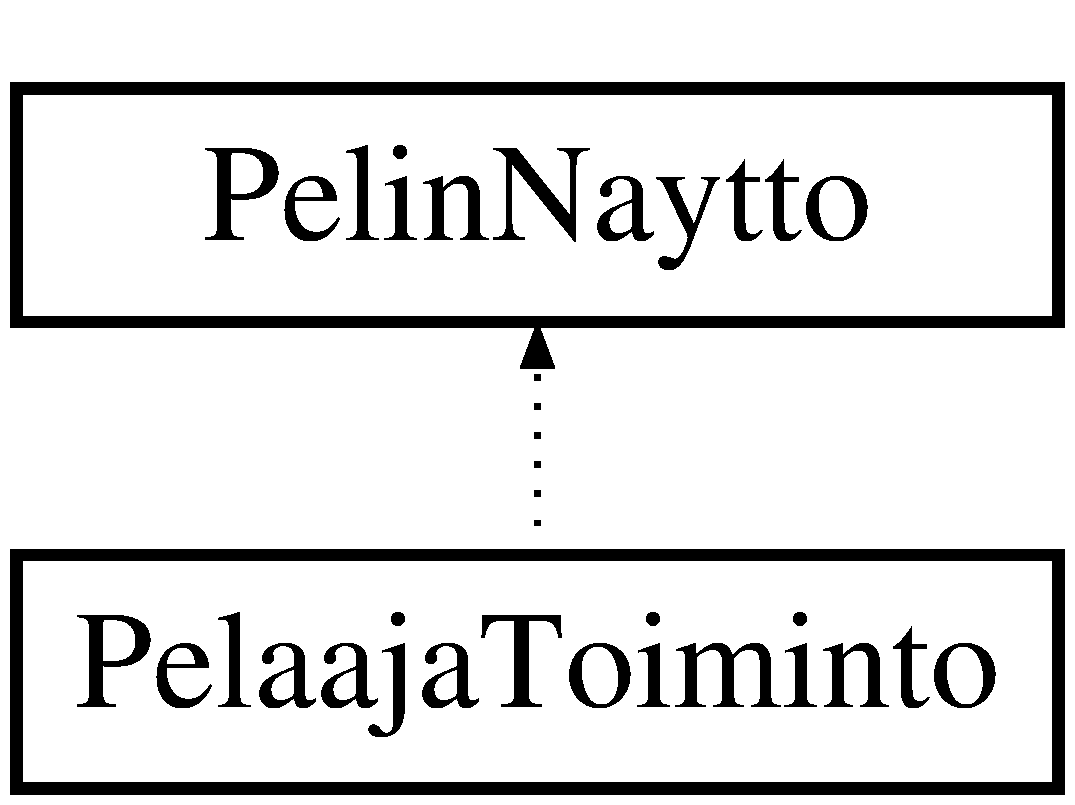
\includegraphics[height=2.000000cm]{class_pelin_naytto}
\end{center}
\end{figure}
\subsection*{Public Member Functions}
\begin{DoxyCompactItemize}
\item 
\hyperlink{class_pelin_naytto_a69dd5937c265b77376e79368a066dd99}{Pelin\+Naytto} (\hyperlink{class_julkinen_1_1_nayttorajapinta}{Julkinen\+::\+Nayttorajapinta} $\ast$naytto)
\begin{DoxyCompactList}\small\item\em \hyperlink{class_pelin_naytto}{Pelin\+Naytto} rakentaja. \end{DoxyCompactList}\item 
\hyperlink{class_pelin_naytto_a9d8dbd0f5e10e826d97cee98fd47247d}{$\sim$\+Pelin\+Naytto} ()
\begin{DoxyCompactList}\small\item\em Purkaja. \end{DoxyCompactList}\item 
void \hyperlink{class_pelin_naytto_a2f155f89cfe6200a727fd45c8aead8c9}{aseta\+Data} (\hyperlink{class_data}{Data} const data)
\begin{DoxyCompactList}\small\item\em Pelidatan asettaja. \end{DoxyCompactList}\item 
void \hyperlink{class_pelin_naytto_a97b89437cac4b6d4edcdb8eb7fe59be4}{aloita\+Rakennus} ()
\begin{DoxyCompactList}\small\item\em Rakennuksen aloittaja. \end{DoxyCompactList}\item 
void \hyperlink{class_pelin_naytto_a2c925cc22e2a633889a8bcebd40e9708}{lopeta\+Rakennus} ()
\begin{DoxyCompactList}\small\item\em Rakennuksen lopettaja. \end{DoxyCompactList}\item 
void \hyperlink{class_pelin_naytto_adc943c511334eb5be52dc93e4eccb52c}{vuorossa} (std\+::string const \&nimi)
\begin{DoxyCompactList}\small\item\em Vuorossa olevan tulostaja. \end{DoxyCompactList}\item 
void \hyperlink{class_pelin_naytto_a06f0e63f3e8bfe7010f4a2f599e8b3b6}{ilmoitus\+Erikoispalaan\+Astuttu} (\hyperlink{class_pala}{Pala} const pala, \hyperlink{class_pelaaja}{Pelaaja} const pelaaja)
\begin{DoxyCompactList}\small\item\em Erikoispalaan astumisesta ilmoittaja. \end{DoxyCompactList}\item 
void \hyperlink{class_pelin_naytto_adf20b1b8e047f0f2c0c774e1919b413e}{ilmoitus\+Esine\+Poimittu} (\hyperlink{class_esine}{Esine} const esine)
\begin{DoxyCompactList}\small\item\em Esineen poiminnasta ilmoittaja. \end{DoxyCompactList}\item 
void \hyperlink{class_pelin_naytto_a9c79b538f5e79bfd42a93c10340d7369}{tulosta\+Virhe} (\hyperlink{class_julkinen_1_1_toimintovirhe}{Julkinen\+::\+Toimintovirhe} virhe)
\begin{DoxyCompactList}\small\item\em Virheen tulostaja. \end{DoxyCompactList}\end{DoxyCompactItemize}


\subsection{Detailed Description}
Labyrintti-\/pelin pelin toimintojen näyttöön piirtäjä. 

\subsection{Constructor \& Destructor Documentation}
\hypertarget{class_pelin_naytto_a69dd5937c265b77376e79368a066dd99}{}\index{Pelin\+Naytto@{Pelin\+Naytto}!Pelin\+Naytto@{Pelin\+Naytto}}
\index{Pelin\+Naytto@{Pelin\+Naytto}!Pelin\+Naytto@{Pelin\+Naytto}}
\subsubsection[{Pelin\+Naytto(\+Julkinen\+::\+Nayttorajapinta $\ast$naytto)}]{\setlength{\rightskip}{0pt plus 5cm}Pelin\+Naytto\+::\+Pelin\+Naytto (
\begin{DoxyParamCaption}
\item[{{\bf Julkinen\+::\+Nayttorajapinta} $\ast$}]{naytto}
\end{DoxyParamCaption}
)}\label{class_pelin_naytto_a69dd5937c265b77376e79368a066dd99}


\hyperlink{class_pelin_naytto}{Pelin\+Naytto} rakentaja. 

\begin{DoxyPrecond}{Precondition}
Annettu osoite näyttöön on kelvollinen.
\end{DoxyPrecond}
Asettaa käytettävän näytön.


\begin{DoxyParams}[1]{Parameters}
\mbox{\tt in}  & {\em naytto} & Käytettävä näyttö {\ttfamily \hyperlink{class_julkinen_1_1_nayttorajapinta}{Julkinen\+::\+Nayttorajapinta}}-\/luokkan osoitteena. \\
\hline
\end{DoxyParams}
\hypertarget{class_pelin_naytto_a9d8dbd0f5e10e826d97cee98fd47247d}{}\index{Pelin\+Naytto@{Pelin\+Naytto}!````~Pelin\+Naytto@{$\sim$\+Pelin\+Naytto}}
\index{````~Pelin\+Naytto@{$\sim$\+Pelin\+Naytto}!Pelin\+Naytto@{Pelin\+Naytto}}
\subsubsection[{$\sim$\+Pelin\+Naytto()}]{\setlength{\rightskip}{0pt plus 5cm}Pelin\+Naytto\+::$\sim$\+Pelin\+Naytto (
\begin{DoxyParamCaption}
{}
\end{DoxyParamCaption}
)}\label{class_pelin_naytto_a9d8dbd0f5e10e826d97cee98fd47247d}


Purkaja. 

\begin{DoxyPostcond}{Postcondition}
No-\/throw takuu. 
\end{DoxyPostcond}


\subsection{Member Function Documentation}
\hypertarget{class_pelin_naytto_a97b89437cac4b6d4edcdb8eb7fe59be4}{}\index{Pelin\+Naytto@{Pelin\+Naytto}!aloita\+Rakennus@{aloita\+Rakennus}}
\index{aloita\+Rakennus@{aloita\+Rakennus}!Pelin\+Naytto@{Pelin\+Naytto}}
\subsubsection[{aloita\+Rakennus()}]{\setlength{\rightskip}{0pt plus 5cm}void Pelin\+Naytto\+::aloita\+Rakennus (
\begin{DoxyParamCaption}
{}
\end{DoxyParamCaption}
)}\label{class_pelin_naytto_a97b89437cac4b6d4edcdb8eb7fe59be4}


Rakennuksen aloittaja. 

Käskee osoitettua {\ttfamily \hyperlink{class_julkinen_1_1_nayttorajapinta}{Julkinen\+::\+Nayttorajapinta}}-\/luokkaa aloittamaan rakennuksen.

\begin{DoxyPostcond}{Postcondition}
Osoitettua {\ttfamily \hyperlink{class_julkinen_1_1_nayttorajapinta}{Julkinen\+::\+Nayttorajapinta}}-\/luokka rakennus tilassa. 
\end{DoxyPostcond}
\hypertarget{class_pelin_naytto_a2f155f89cfe6200a727fd45c8aead8c9}{}\index{Pelin\+Naytto@{Pelin\+Naytto}!aseta\+Data@{aseta\+Data}}
\index{aseta\+Data@{aseta\+Data}!Pelin\+Naytto@{Pelin\+Naytto}}
\subsubsection[{aseta\+Data(\+Data const data)}]{\setlength{\rightskip}{0pt plus 5cm}void Pelin\+Naytto\+::aseta\+Data (
\begin{DoxyParamCaption}
\item[{{\bf Data} const}]{data}
\end{DoxyParamCaption}
)}\label{class_pelin_naytto_a2f155f89cfe6200a727fd45c8aead8c9}


Pelidatan asettaja. 

Asettaa käytettävän datan.


\begin{DoxyParams}[1]{Parameters}
\mbox{\tt in}  & {\em data} & Käytettävä data {\ttfamily \hyperlink{class_data}{Data}}-\/luokkana. \\
\hline
\end{DoxyParams}
\hypertarget{class_pelin_naytto_a06f0e63f3e8bfe7010f4a2f599e8b3b6}{}\index{Pelin\+Naytto@{Pelin\+Naytto}!ilmoitus\+Erikoispalaan\+Astuttu@{ilmoitus\+Erikoispalaan\+Astuttu}}
\index{ilmoitus\+Erikoispalaan\+Astuttu@{ilmoitus\+Erikoispalaan\+Astuttu}!Pelin\+Naytto@{Pelin\+Naytto}}
\subsubsection[{ilmoitus\+Erikoispalaan\+Astuttu(\+Pala const pala, Pelaaja const pelaaja)}]{\setlength{\rightskip}{0pt plus 5cm}void Pelin\+Naytto\+::ilmoitus\+Erikoispalaan\+Astuttu (
\begin{DoxyParamCaption}
\item[{{\bf Pala} const}]{pala, }
\item[{{\bf Pelaaja} const}]{pelaaja}
\end{DoxyParamCaption}
)}\label{class_pelin_naytto_a06f0e63f3e8bfe7010f4a2f599e8b3b6}


Erikoispalaan astumisesta ilmoittaja. 

Kertoo {\ttfamily \hyperlink{class_julkinen_1_1_nayttorajapinta}{Julkinen\+::\+Nayttorajapinta}}-\/luokkalle kuka astui mihin erikoispalaan.


\begin{DoxyParams}[1]{Parameters}
\mbox{\tt in}  & {\em pala} & Astuttu pala {\ttfamily \hyperlink{class_pala}{Pala}}-\/luokkana. \\
\hline
\mbox{\tt in}  & {\em pelaaja} & Astunut pelaaja {\ttfamily \hyperlink{class_pelaaja}{Pelaaja}}-\/luokkana \\
\hline
\end{DoxyParams}
\hypertarget{class_pelin_naytto_adf20b1b8e047f0f2c0c774e1919b413e}{}\index{Pelin\+Naytto@{Pelin\+Naytto}!ilmoitus\+Esine\+Poimittu@{ilmoitus\+Esine\+Poimittu}}
\index{ilmoitus\+Esine\+Poimittu@{ilmoitus\+Esine\+Poimittu}!Pelin\+Naytto@{Pelin\+Naytto}}
\subsubsection[{ilmoitus\+Esine\+Poimittu(\+Esine const esine)}]{\setlength{\rightskip}{0pt plus 5cm}void Pelin\+Naytto\+::ilmoitus\+Esine\+Poimittu (
\begin{DoxyParamCaption}
\item[{{\bf Esine} const}]{esine}
\end{DoxyParamCaption}
)}\label{class_pelin_naytto_adf20b1b8e047f0f2c0c774e1919b413e}


Esineen poiminnasta ilmoittaja. 

Kertoo {\ttfamily \hyperlink{class_julkinen_1_1_nayttorajapinta}{Julkinen\+::\+Nayttorajapinta}}-\/luokkalle kuka poimi minkä esineen.


\begin{DoxyParams}[1]{Parameters}
\mbox{\tt in}  & {\em esine} & Poimittu esine {\ttfamily \hyperlink{class_esine}{Esine}}-\/luokkana. \\
\hline
\end{DoxyParams}
\hypertarget{class_pelin_naytto_a2c925cc22e2a633889a8bcebd40e9708}{}\index{Pelin\+Naytto@{Pelin\+Naytto}!lopeta\+Rakennus@{lopeta\+Rakennus}}
\index{lopeta\+Rakennus@{lopeta\+Rakennus}!Pelin\+Naytto@{Pelin\+Naytto}}
\subsubsection[{lopeta\+Rakennus()}]{\setlength{\rightskip}{0pt plus 5cm}void Pelin\+Naytto\+::lopeta\+Rakennus (
\begin{DoxyParamCaption}
{}
\end{DoxyParamCaption}
)}\label{class_pelin_naytto_a2c925cc22e2a633889a8bcebd40e9708}


Rakennuksen lopettaja. 

\begin{DoxyPrecond}{Precondition}
Osoitettu {\ttfamily \hyperlink{class_julkinen_1_1_nayttorajapinta}{Julkinen\+::\+Nayttorajapinta}}-\/luokka on rakennustilassa.
\end{DoxyPrecond}
Asettaa kaiken datan näytölle ja lopettaa rakennuksen.

\begin{DoxyPostcond}{Postcondition}
Kaikki data näytöllä. Osoitettua {\ttfamily \hyperlink{class_julkinen_1_1_nayttorajapinta}{Julkinen\+::\+Nayttorajapinta}}-\/luokka tulostus tilassa. 
\end{DoxyPostcond}
\hypertarget{class_pelin_naytto_a9c79b538f5e79bfd42a93c10340d7369}{}\index{Pelin\+Naytto@{Pelin\+Naytto}!tulosta\+Virhe@{tulosta\+Virhe}}
\index{tulosta\+Virhe@{tulosta\+Virhe}!Pelin\+Naytto@{Pelin\+Naytto}}
\subsubsection[{tulosta\+Virhe(\+Julkinen\+::\+Toimintovirhe virhe)}]{\setlength{\rightskip}{0pt plus 5cm}void Pelin\+Naytto\+::tulosta\+Virhe (
\begin{DoxyParamCaption}
\item[{{\bf Julkinen\+::\+Toimintovirhe}}]{virhe}
\end{DoxyParamCaption}
)}\label{class_pelin_naytto_a9c79b538f5e79bfd42a93c10340d7369}


Virheen tulostaja. 

Tulostaa toimintavirheen.


\begin{DoxyParams}[1]{Parameters}
\mbox{\tt in}  & {\em virhe} & Tulostettava virhe {\ttfamily \hyperlink{class_julkinen_1_1_toimintovirhe}{Julkinen\+::\+Toimintovirhe}}-\/luokkana. \\
\hline
\end{DoxyParams}
\hypertarget{class_pelin_naytto_adc943c511334eb5be52dc93e4eccb52c}{}\index{Pelin\+Naytto@{Pelin\+Naytto}!vuorossa@{vuorossa}}
\index{vuorossa@{vuorossa}!Pelin\+Naytto@{Pelin\+Naytto}}
\subsubsection[{vuorossa(std\+::string const \&nimi)}]{\setlength{\rightskip}{0pt plus 5cm}void Pelin\+Naytto\+::vuorossa (
\begin{DoxyParamCaption}
\item[{std\+::string const \&}]{nimi}
\end{DoxyParamCaption}
)}\label{class_pelin_naytto_adc943c511334eb5be52dc93e4eccb52c}


Vuorossa olevan tulostaja. 

Kertoo {\ttfamily \hyperlink{class_julkinen_1_1_nayttorajapinta}{Julkinen\+::\+Nayttorajapinta}}-\/luokkalle kuka on vuorossa.


\begin{DoxyParams}[1]{Parameters}
\mbox{\tt in}  & {\em nimi} & {\ttfamily Vuorossa} olevan pelaajan nimi. \\
\hline
\end{DoxyParams}


The documentation for this class was generated from the following files\+:\begin{DoxyCompactItemize}
\item 
\hyperlink{_pelin_naytto_8hpp}{Pelin\+Naytto.\+hpp}\item 
Pelin\+Naytto.\+cpp\end{DoxyCompactItemize}

\hypertarget{class_julkinen_1_1_pelirajapinta}{}\section{Julkinen\+:\+:Pelirajapinta Class Reference}
\label{class_julkinen_1_1_pelirajapinta}\index{Julkinen\+::\+Pelirajapinta@{Julkinen\+::\+Pelirajapinta}}


Labyrintti-\/pelin ohjausrajapinta.  




{\ttfamily \#include $<$pelirajapinta.\+hh$>$}

Inheritance diagram for Julkinen\+:\+:Pelirajapinta\+:\begin{figure}[H]
\begin{center}
\leavevmode
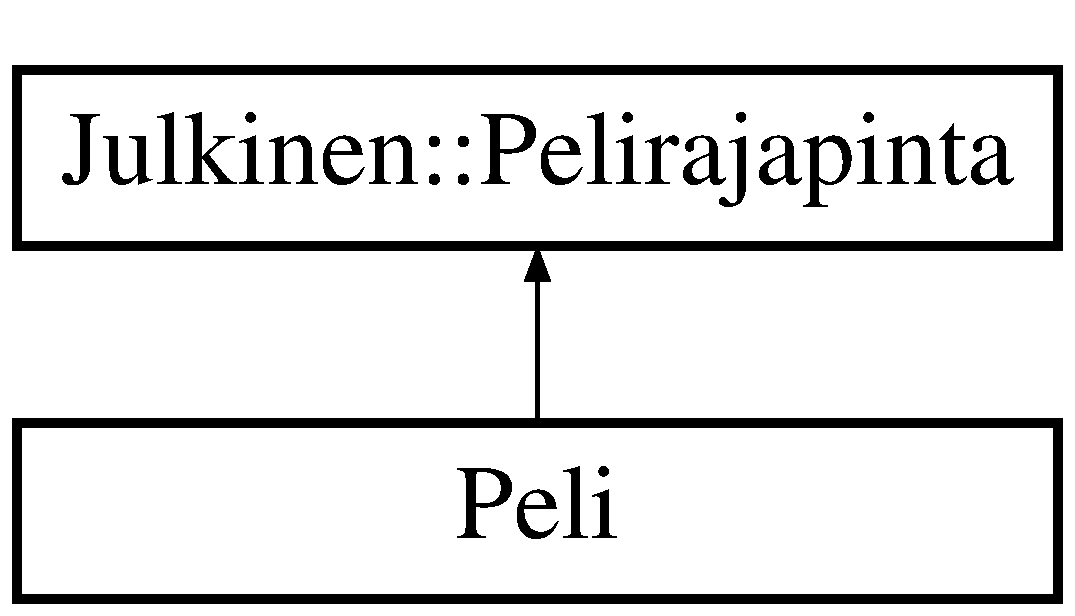
\includegraphics[height=2.000000cm]{class_julkinen_1_1_pelirajapinta}
\end{center}
\end{figure}
\subsection*{Public Member Functions}
\begin{DoxyCompactItemize}
\item 
\hyperlink{class_julkinen_1_1_pelirajapinta_a9d639630818d96bdea435e2f36eb667a}{Pelirajapinta} ()
\begin{DoxyCompactList}\small\item\em Oletusrakentaja. \end{DoxyCompactList}\item 
virtual \hyperlink{class_julkinen_1_1_pelirajapinta_acc26ce5341e1a73dff4f3c1e2968b803}{$\sim$\+Pelirajapinta} ()
\begin{DoxyCompactList}\small\item\em Tuhoaja. \end{DoxyCompactList}\item 
virtual bool \hyperlink{class_julkinen_1_1_pelirajapinta_a8e1aafabbb4bd5803d10672d8ad33450}{onko\+Alustustilassa} () const  =0
\begin{DoxyCompactList}\small\item\em Kertoo onko peli alustustilassa. \end{DoxyCompactList}\item 
virtual void \hyperlink{class_julkinen_1_1_pelirajapinta_ad1597bf68505144431c62cc7c6e49bf6}{lisaa\+Naytto} (\hyperlink{class_julkinen_1_1_nayttorajapinta}{Nayttorajapinta} $\ast$naytto)=0
\begin{DoxyCompactList}\small\item\em Lisaa tulostus olion peliin. \end{DoxyCompactList}\item 
virtual void \hyperlink{class_julkinen_1_1_pelirajapinta_aeaa98dab134d9345ef33fbf92224702e}{maarita\+Pelialueen\+Koko} (\hyperlink{class_julkinen_1_1_koordinaatti}{Julkinen\+::\+Koordinaatti} const \&koko)=0
\begin{DoxyCompactList}\small\item\em Maarittaa pelikentän koon. \end{DoxyCompactList}\item 
virtual void \hyperlink{class_julkinen_1_1_pelirajapinta_ac060096b71a764e75436c0dea146b1ef}{lisaa\+Pelaaja} (\hyperlink{namespace_julkinen_ad9a0a9e01af78249f584a93b03db4329}{Pelaaja\+Tyyppi} tyyppi, std\+::string const \&nimi, char lyhenne, \hyperlink{class_julkinen_1_1_koordinaatti}{Julkinen\+::\+Koordinaatti} const \&sijainti)=0
\begin{DoxyCompactList}\small\item\em Pelin alustusfunktio, joka lisaa pelaajan peliin. \end{DoxyCompactList}\item 
virtual void \hyperlink{class_julkinen_1_1_pelirajapinta_a149820998333ec4d7fa9fd3ff5ea98fd}{lisaa\+Pala} (\hyperlink{namespace_julkinen_a272c70e0503191a485c8a9cd4281e6f5}{Pala\+Tyyppi} pala, unsigned int rotaatio, \hyperlink{class_julkinen_1_1_koordinaatti}{Julkinen\+::\+Koordinaatti} const \&sijainti)=0
\begin{DoxyCompactList}\small\item\em Pelin alustusfunktio, joka lisaa palan peliin. \end{DoxyCompactList}\item 
virtual void \hyperlink{class_julkinen_1_1_pelirajapinta_a998c0b644b8b1b73ac74390afea03da9}{lisaa\+Esine} (char merkki, \hyperlink{class_julkinen_1_1_koordinaatti}{Julkinen\+::\+Koordinaatti} const \&sijainti, std\+::string const \&pelaaja)=0
\begin{DoxyCompactList}\small\item\em Pelin alustusfunktio, joka lisaa esineen peliin. \end{DoxyCompactList}\item 
virtual void \hyperlink{class_julkinen_1_1_pelirajapinta_a4de5389102fb5a479173cc3728b989dd}{aseta\+Palan\+Tyyppi} (\hyperlink{namespace_julkinen_afc26052e09d0b2214f749492cc5fff19}{Julkinen\+::\+Erikoispala\+Tyyppi} tyyppi, \hyperlink{class_julkinen_1_1_koordinaatti}{Julkinen\+::\+Koordinaatti} const \&sijainti, \hyperlink{class_julkinen_1_1_koordinaatti}{Julkinen\+::\+Koordinaatti} const \&kohde=\hyperlink{class_julkinen_1_1_koordinaatti}{Julkinen\+::\+Koordinaatti}())=0
\begin{DoxyCompactList}\small\item\em Pelin alustusfunktio, joka asettaa palan erikoispalan tyypin. \end{DoxyCompactList}\item 
virtual void \hyperlink{class_julkinen_1_1_pelirajapinta_afdcc11ea245937075026e82be6e9a874}{alustus\+Lopeta} ()=0
\begin{DoxyCompactList}\small\item\em Lopettaa pelin alustuksen. \end{DoxyCompactList}\item 
virtual bool \hyperlink{class_julkinen_1_1_pelirajapinta_a3f8d4b6037d2370242f3018c3919c4e2}{onko\+Pelitilassa} () const  =0
\begin{DoxyCompactList}\small\item\em Kertoo onko peli pelitilassa. \end{DoxyCompactList}\item 
virtual void \hyperlink{class_julkinen_1_1_pelirajapinta_aea8cbb43bcf85664b97d17df1666ce9f}{komento\+Tyonna} (\hyperlink{namespace_julkinen_acce0eefc4c90f907dd5fb319b0d05872}{Reuna} reuna, unsigned int paikka, unsigned int rotaatio)=0
\begin{DoxyCompactList}\small\item\em Työntää irtopalan annettuun kohtaan. \end{DoxyCompactList}\item 
virtual void \hyperlink{class_julkinen_1_1_pelirajapinta_a3444c155143baff73521a0707712b36a}{komento\+Liiku} (\hyperlink{namespace_julkinen_a81b50e3c6f21c0c1c46e186592107c3c}{Suunta} suunta, unsigned int maara=0)=0
\begin{DoxyCompactList}\small\item\em Liikuttaa vuorossa olevaa pelaajaa. \end{DoxyCompactList}\item 
virtual bool \hyperlink{class_julkinen_1_1_pelirajapinta_a873b4d57d698b82df131246df85c3193}{vaihda\+Vuoro} ()=0
\begin{DoxyCompactList}\small\item\em Vaihtaa vuoron seuraavalle pelaajalle ja ilmoittaa, jatketaanko peliä, vai onko jokin pelaaja voittanut pelin. {\bfseries Huom!} Raakilepalautuksessa tulkitaan, että kukaan ei voita peliä koskaan (koska kerättäviä esineitä ei ole). \end{DoxyCompactList}\item 
virtual \hyperlink{namespace_julkinen_ad9a0a9e01af78249f584a93b03db4329}{Pelaaja\+Tyyppi} \hyperlink{class_julkinen_1_1_pelirajapinta_aef0e254fd13ac8a44bb9db0908daa0e7}{hae\+Vuorossa} ()=0
\begin{DoxyCompactList}\small\item\em Palauttaa vuorossa olevan pelaajan tyypin. \end{DoxyCompactList}\end{DoxyCompactItemize}


\subsection{Detailed Description}
Labyrintti-\/pelin ohjausrajapinta. 

Tämän rajapinnan läpi pelin pääohjelma pystyy ohjaamaan pelin toiminta logiikaa. Pääohjelman vastuulla on pelin alustustiedoston lukeminen ja komentotulkin pyörittäminen.

\hyperlink{class_peli}{Peli} voi olla kahdessa eri tilassa, alustustilassa ja pelitilassa. Kun peli-\/olio luodaan se on alustustilassa ja sille voidaan syöttää peliin liittyvät tiedot, kuten pelialueen koko, pelaajat, palat ja esineet. Kun peli on alustustilassa ei pelivuoroihin liittyviä toiminnalluuksia voida ajaa.

\hyperlink{class_peli}{Peli} alustetaan kutsumalla ensiksi \hyperlink{class_julkinen_1_1_pelirajapinta_ad1597bf68505144431c62cc7c6e49bf6}{lisaa\+Naytto()} metodia, jolla peli liitetään tulostusrajapintaan. Näytön lisäyksen jälkeen kutsutaan \hyperlink{class_julkinen_1_1_pelirajapinta_aeaa98dab134d9345ef33fbf92224702e}{maarita\+Pelialueen\+Koko()} metodia, jolla kerrotaan kuinka suuri pelialue pelissä on. Tämän jälkeen peliin lisätään palat ja pelaajat kutsumalla jokaiselle palalle ja pelaajalle lisaa\+Pala tai lisaa\+Pelaaja metodeja. Kun palat ja pelaajat on lisätty, niin peliin lisätään esineet kutsumalla lisaa\+Esine metodia jokaiselle esineelle. Kun alustus on suoritettu loppuun kutsutaan alustus\+Lopeta metodia.

Peliä pelataan, niin että pelaaja vuorollaan työntää irtopalan \hyperlink{class_julkinen_1_1_pelirajapinta_aea8cbb43bcf85664b97d17df1666ce9f}{komento\+Tyonna()} metodilla ja tämän jälkeen pelaaja liikkuu \hyperlink{class_julkinen_1_1_pelirajapinta_a3444c155143baff73521a0707712b36a}{komento\+Liiku()} metodilla. Poikkeuksena yllä olevaan on tietokone-\/ pelaaja, joka ei välttämättä työnnä palaa vuorollaan vaan käyttää automaatti-\/liikkumista. Pelaajan vuoron lopuksi kutsutaan \hyperlink{class_julkinen_1_1_pelirajapinta_a873b4d57d698b82df131246df85c3193}{vaihda\+Vuoro()}-\/metodia. \begin{DoxyVerb}    Poikkeuksista bac_alloc saa vuotaa ulos, jos muisti loppuu. Käytännössä
    tämä tarkoittaa sitä, että muistin loppumiseen ei välttämättä tarvitse 
    varautua.

    Muistin loppumisesta sekä näyttörajapinnan heittämistä poikkeuksista tarjotaan minimitakuu.\end{DoxyVerb}
 

\subsection{Constructor \& Destructor Documentation}
\hypertarget{class_julkinen_1_1_pelirajapinta_a9d639630818d96bdea435e2f36eb667a}{}\index{Julkinen\+::\+Pelirajapinta@{Julkinen\+::\+Pelirajapinta}!Pelirajapinta@{Pelirajapinta}}
\index{Pelirajapinta@{Pelirajapinta}!Julkinen\+::\+Pelirajapinta@{Julkinen\+::\+Pelirajapinta}}
\subsubsection[{Pelirajapinta()}]{\setlength{\rightskip}{0pt plus 5cm}Julkinen\+::\+Pelirajapinta\+::\+Pelirajapinta (
\begin{DoxyParamCaption}
{}
\end{DoxyParamCaption}
)\hspace{0.3cm}{\ttfamily [inline]}}\label{class_julkinen_1_1_pelirajapinta_a9d639630818d96bdea435e2f36eb667a}


Oletusrakentaja. 

Tämä rakentaja on määritelty, jotta voidaan dokumentoida Pelirajapinnan tila pelin luomisen jälkeen. \begin{DoxyVerb}        \pre -
\end{DoxyVerb}
 \begin{DoxyPostcond}{Postcondition}
\hyperlink{class_peli}{Peli} on alustustilassa ja sen alustaminen voidaan aloittaa. Poikkeustakuu\+: Poikkeuksen sattuessa Pelirajapinta-\/olion luonti epäonnistui, mistä syytä oliolla ei ole sisäistä tilaa jolle voisi antaa takuita. 
\end{DoxyPostcond}
\hypertarget{class_julkinen_1_1_pelirajapinta_acc26ce5341e1a73dff4f3c1e2968b803}{}\index{Julkinen\+::\+Pelirajapinta@{Julkinen\+::\+Pelirajapinta}!````~Pelirajapinta@{$\sim$\+Pelirajapinta}}
\index{````~Pelirajapinta@{$\sim$\+Pelirajapinta}!Julkinen\+::\+Pelirajapinta@{Julkinen\+::\+Pelirajapinta}}
\subsubsection[{$\sim$\+Pelirajapinta()}]{\setlength{\rightskip}{0pt plus 5cm}virtual Julkinen\+::\+Pelirajapinta\+::$\sim$\+Pelirajapinta (
\begin{DoxyParamCaption}
{}
\end{DoxyParamCaption}
)\hspace{0.3cm}{\ttfamily [inline]}, {\ttfamily [virtual]}}\label{class_julkinen_1_1_pelirajapinta_acc26ce5341e1a73dff4f3c1e2968b803}


Tuhoaja. 

\begin{DoxyPrecond}{Precondition}
-\/ 
\end{DoxyPrecond}
\begin{DoxyPostcond}{Postcondition}
No-\/throw takuu. 
\end{DoxyPostcond}


\subsection{Member Function Documentation}
\hypertarget{class_julkinen_1_1_pelirajapinta_afdcc11ea245937075026e82be6e9a874}{}\index{Julkinen\+::\+Pelirajapinta@{Julkinen\+::\+Pelirajapinta}!alustus\+Lopeta@{alustus\+Lopeta}}
\index{alustus\+Lopeta@{alustus\+Lopeta}!Julkinen\+::\+Pelirajapinta@{Julkinen\+::\+Pelirajapinta}}
\subsubsection[{alustus\+Lopeta()=0}]{\setlength{\rightskip}{0pt plus 5cm}virtual void Julkinen\+::\+Pelirajapinta\+::alustus\+Lopeta (
\begin{DoxyParamCaption}
{}
\end{DoxyParamCaption}
)\hspace{0.3cm}{\ttfamily [pure virtual]}}\label{class_julkinen_1_1_pelirajapinta_afdcc11ea245937075026e82be6e9a874}


Lopettaa pelin alustuksen. 

\begin{DoxyPrecond}{Precondition}
\hyperlink{class_peli}{Peli} on alustettu. 
\end{DoxyPrecond}
\begin{DoxyPostcond}{Postcondition}
\hyperlink{class_peli}{Peli} on pelitilassa. Poikkeustakuu\+: Perustakuu poikkeuksen sattuessa. 
\end{DoxyPostcond}


Implemented in \hyperlink{class_peli_a65eff799de42881efc08f7994b27968e}{Peli}.

\hypertarget{class_julkinen_1_1_pelirajapinta_a4de5389102fb5a479173cc3728b989dd}{}\index{Julkinen\+::\+Pelirajapinta@{Julkinen\+::\+Pelirajapinta}!aseta\+Palan\+Tyyppi@{aseta\+Palan\+Tyyppi}}
\index{aseta\+Palan\+Tyyppi@{aseta\+Palan\+Tyyppi}!Julkinen\+::\+Pelirajapinta@{Julkinen\+::\+Pelirajapinta}}
\subsubsection[{aseta\+Palan\+Tyyppi(\+Julkinen\+::\+Erikoispala\+Tyyppi tyyppi, Julkinen\+::\+Koordinaatti const \&sijainti, Julkinen\+::\+Koordinaatti const \&kohde=\+Julkinen\+::\+Koordinaatti())=0}]{\setlength{\rightskip}{0pt plus 5cm}virtual void Julkinen\+::\+Pelirajapinta\+::aseta\+Palan\+Tyyppi (
\begin{DoxyParamCaption}
\item[{{\bf Julkinen\+::\+Erikoispala\+Tyyppi}}]{tyyppi, }
\item[{{\bf Julkinen\+::\+Koordinaatti} const \&}]{sijainti, }
\item[{{\bf Julkinen\+::\+Koordinaatti} const \&}]{kohde = {\ttfamily {\bf Julkinen\+::\+Koordinaatti}()}}
\end{DoxyParamCaption}
)\hspace{0.3cm}{\ttfamily [pure virtual]}}\label{class_julkinen_1_1_pelirajapinta_a4de5389102fb5a479173cc3728b989dd}


Pelin alustusfunktio, joka asettaa palan erikoispalan tyypin. 

\begin{DoxyPrecond}{Precondition}
\hyperlink{class_peli}{Peli} on alustustilassa. Pelilauta ja palat on alustettu. 
\end{DoxyPrecond}
\begin{DoxyPostcond}{Postcondition}
Palan erikoisominaisuudet on luotu. Poikkeustakuu\+: Perustakuu poikkeuksen sattuessa.
\end{DoxyPostcond}

\begin{DoxyParams}[1]{Parameters}
\mbox{\tt in}  & {\em tyyppi} & Palan erikoistyyppi, joka kertoo onko pala normaali, teleportti, siunattu tai kirottu. \\
\hline
\mbox{\tt in}  & {\em sijainti} & Kertoo mitä labyrintin palaa käsitellään. \\
\hline
\mbox{\tt in}  & {\em kohde} & Teleportti-\/palan kohderuudun koordinaatti, muilla paloilla parametria ei anneta.\\
\hline
\end{DoxyParams}

\begin{DoxyExceptions}{Exceptions}
{\em \hyperlink{class_julkinen_1_1_alustusvirhe}{Alustusvirhe}} & Annettu koordinaatti on pelialueen ulkopuolella. \\
\hline
\end{DoxyExceptions}


Implemented in \hyperlink{class_peli_a8045f08b5aa05114baced0541142e735}{Peli}.

\hypertarget{class_julkinen_1_1_pelirajapinta_aef0e254fd13ac8a44bb9db0908daa0e7}{}\index{Julkinen\+::\+Pelirajapinta@{Julkinen\+::\+Pelirajapinta}!hae\+Vuorossa@{hae\+Vuorossa}}
\index{hae\+Vuorossa@{hae\+Vuorossa}!Julkinen\+::\+Pelirajapinta@{Julkinen\+::\+Pelirajapinta}}
\subsubsection[{hae\+Vuorossa()=0}]{\setlength{\rightskip}{0pt plus 5cm}virtual {\bf Pelaaja\+Tyyppi} Julkinen\+::\+Pelirajapinta\+::hae\+Vuorossa (
\begin{DoxyParamCaption}
{}
\end{DoxyParamCaption}
)\hspace{0.3cm}{\ttfamily [pure virtual]}}\label{class_julkinen_1_1_pelirajapinta_aef0e254fd13ac8a44bb9db0908daa0e7}


Palauttaa vuorossa olevan pelaajan tyypin. 

\begin{DoxyPrecond}{Precondition}
\hyperlink{class_peli}{Peli} on pelitilassa. 
\end{DoxyPrecond}
\begin{DoxyPostcond}{Postcondition}
\hyperlink{class_peli}{Peli} on pelitilassa ja vuorossa olevan pelaajan {\ttfamily Pelaaja\+Tyyppi} on palautettu. Poikkeustakuu\+: No-\/throw takuu.
\end{DoxyPostcond}
\begin{DoxyReturn}{Returns}
Palauttaa vuorossa olevan pelaajan {\ttfamily Pelaaja\+Tyyppi}. 
\end{DoxyReturn}


Implemented in \hyperlink{class_peli_a43524af1c4c914acc5faf872b5dcf890}{Peli}.

\hypertarget{class_julkinen_1_1_pelirajapinta_a3444c155143baff73521a0707712b36a}{}\index{Julkinen\+::\+Pelirajapinta@{Julkinen\+::\+Pelirajapinta}!komento\+Liiku@{komento\+Liiku}}
\index{komento\+Liiku@{komento\+Liiku}!Julkinen\+::\+Pelirajapinta@{Julkinen\+::\+Pelirajapinta}}
\subsubsection[{komento\+Liiku(\+Suunta suunta, unsigned int maara=0)=0}]{\setlength{\rightskip}{0pt plus 5cm}virtual void Julkinen\+::\+Pelirajapinta\+::komento\+Liiku (
\begin{DoxyParamCaption}
\item[{{\bf Suunta}}]{suunta, }
\item[{unsigned int}]{maara = {\ttfamily 0}}
\end{DoxyParamCaption}
)\hspace{0.3cm}{\ttfamily [pure virtual]}}\label{class_julkinen_1_1_pelirajapinta_a3444c155143baff73521a0707712b36a}


Liikuttaa vuorossa olevaa pelaajaa. 

Liikuttaa vuorossa olevaa pelaajaa annettuun suuntaan annetun määrän. Jos pelaaja ei pysty liikkumaan annettuun suuntaan annettua määrää heitetään \hyperlink{class_julkinen_1_1_toimintovirhe}{Toimintovirhe}. \hyperlink{class_julkinen_1_1_toimintovirhe}{Toimintovirhe} heitetään myös silloin jos pelaaja ei ole työntänyt palaa tällä vuorolla, paitsi jos suunta on A\+U\+T\+O\+M\+A\+A\+T\+T\+I. Raakilepalautuksessa liikkuminen suoritetaan, vaikka työntämistä ei olekaan suoritettu (eli poikkeusta ei heitetä).

\begin{DoxyPrecond}{Precondition}
\hyperlink{class_peli}{Peli} on pelitilassa. 
\end{DoxyPrecond}
\begin{DoxyPostcond}{Postcondition}
\hyperlink{class_pelaaja}{Pelaaja} on liikutettu ja pelilauta on tulostettu uudestaan. Poikkeustakuu\+: Vahvatakuu \hyperlink{class_julkinen_1_1_komentovirhe}{Komentovirhe} tai \hyperlink{class_julkinen_1_1_toimintovirhe}{Toimintovirhe} poikkeuksen sattuessa.
\end{DoxyPostcond}

\begin{DoxyParams}[1]{Parameters}
\mbox{\tt in}  & {\em suunta} & Suunta johon pelaajaa siirretään. \\
\hline
\mbox{\tt in}  & {\em maara} & Pelaajan liikkumien ruutujen määrä.\\
\hline
\end{DoxyParams}

\begin{DoxyExceptions}{Exceptions}
{\em \hyperlink{class_julkinen_1_1_toimintovirhe}{Toimintovirhe}} & Vuorossa oleva pelaaja ei voi liikkua annettuun suuntaan annettua määrää. \\
\hline
{\em \hyperlink{class_julkinen_1_1_toimintovirhe}{Toimintovirhe}} & Vuorossa oleva pelaaja ei ole työntänyt irtopalaa. Ei heitetä jos suunta on A\+U\+T\+O\+M\+A\+A\+T\+T\+I. Ei heitetä raakilepalautuksessa. \\
\hline
{\em \hyperlink{class_julkinen_1_1_komentovirhe}{Komentovirhe}} & maara on negatiivinen. \\
\hline
{\em \hyperlink{class_julkinen_1_1_komentovirhe}{Komentovirhe}} & maara on 0, mutta suunta ei ole P\+A\+I\+K\+A\+L\+L\+A\+A\+N. \\
\hline
\end{DoxyExceptions}


Implemented in \hyperlink{class_peli_ad721f34f1e12e0dae3e2f73de2d99d05}{Peli}.

\hypertarget{class_julkinen_1_1_pelirajapinta_aea8cbb43bcf85664b97d17df1666ce9f}{}\index{Julkinen\+::\+Pelirajapinta@{Julkinen\+::\+Pelirajapinta}!komento\+Tyonna@{komento\+Tyonna}}
\index{komento\+Tyonna@{komento\+Tyonna}!Julkinen\+::\+Pelirajapinta@{Julkinen\+::\+Pelirajapinta}}
\subsubsection[{komento\+Tyonna(\+Reuna reuna, unsigned int paikka, unsigned int rotaatio)=0}]{\setlength{\rightskip}{0pt plus 5cm}virtual void Julkinen\+::\+Pelirajapinta\+::komento\+Tyonna (
\begin{DoxyParamCaption}
\item[{{\bf Reuna}}]{reuna, }
\item[{unsigned int}]{paikka, }
\item[{unsigned int}]{rotaatio}
\end{DoxyParamCaption}
)\hspace{0.3cm}{\ttfamily [pure virtual]}}\label{class_julkinen_1_1_pelirajapinta_aea8cbb43bcf85664b97d17df1666ce9f}


Työntää irtopalan annettuun kohtaan. 

Raakilepalautuksessa tätä operaatiota ei kutsuta.

\begin{DoxyPrecond}{Precondition}
\hyperlink{class_peli}{Peli} on pelitilassa. 
\end{DoxyPrecond}
\begin{DoxyPostcond}{Postcondition}
Irtopala on asetettu annettuun kohtaan ja työntö kohdan työntösuunnan mukaisen vastapään pala on otettu uudeksi irtopalaksi. Pelilauta on tulostettu uudestaan. Poikkeustakuu\+: Vahvatakuu \hyperlink{class_julkinen_1_1_komentovirhe}{Komentovirhe} poikkeuksen sattuessa.
\end{DoxyPostcond}

\begin{DoxyParams}[1]{Parameters}
\mbox{\tt in}  & {\em reuna} & Reuna jolle pala työnnetään. \\
\hline
\mbox{\tt in}  & {\em rotaatio} & Työnnettävän palan rotaatio (1-\/4) \\
\hline
\mbox{\tt in}  & {\em paikka} & Mihin kohtaan reunaa pala työnnetään.\\
\hline
\end{DoxyParams}

\begin{DoxyExceptions}{Exceptions}
{\em \hyperlink{class_julkinen_1_1_toimintovirhe}{Toimintovirhe}} & \hyperlink{class_pelaaja}{Pelaaja} on jo työntänyt palaa tällä vuorolla. \\
\hline
{\em \hyperlink{class_julkinen_1_1_komentovirhe}{Komentovirhe}} & Paikka on virheellinen. \\
\hline
{\em \hyperlink{class_julkinen_1_1_komentovirhe}{Komentovirhe}} & Rotaatio on virheellinen. \\
\hline
\end{DoxyExceptions}


Implemented in \hyperlink{class_peli_a4093d9ae2c4b220a4da9bcc728f7d59b}{Peli}.

\hypertarget{class_julkinen_1_1_pelirajapinta_a998c0b644b8b1b73ac74390afea03da9}{}\index{Julkinen\+::\+Pelirajapinta@{Julkinen\+::\+Pelirajapinta}!lisaa\+Esine@{lisaa\+Esine}}
\index{lisaa\+Esine@{lisaa\+Esine}!Julkinen\+::\+Pelirajapinta@{Julkinen\+::\+Pelirajapinta}}
\subsubsection[{lisaa\+Esine(char merkki, Julkinen\+::\+Koordinaatti const \&sijainti, std\+::string const \&pelaaja)=0}]{\setlength{\rightskip}{0pt plus 5cm}virtual void Julkinen\+::\+Pelirajapinta\+::lisaa\+Esine (
\begin{DoxyParamCaption}
\item[{char}]{merkki, }
\item[{{\bf Julkinen\+::\+Koordinaatti} const \&}]{sijainti, }
\item[{std\+::string const \&}]{pelaaja}
\end{DoxyParamCaption}
)\hspace{0.3cm}{\ttfamily [pure virtual]}}\label{class_julkinen_1_1_pelirajapinta_a998c0b644b8b1b73ac74390afea03da9}


Pelin alustusfunktio, joka lisaa esineen peliin. 

\begin{DoxyPrecond}{Precondition}
\hyperlink{class_peli}{Peli} on alustustilassa. Pelilauta ja pelaajat on alustettu. 
\end{DoxyPrecond}
\begin{DoxyPostcond}{Postcondition}
\hyperlink{class_esine}{Esine} on lisatty peliin ja mahdollisesti annetulle pelaajalle, esine on lisätty kerättäviin esineisiin. Poikkeustakuu\+: Perustakuu poikkeuksen sattuessa.
\end{DoxyPostcond}

\begin{DoxyParams}[1]{Parameters}
\mbox{\tt in}  & {\em merkki} & Esinettä kuvaava merkki pelissä. \\
\hline
\mbox{\tt in}  & {\em sijainti} & Kertoo mihin labyrintin koordinaattiin esine laitetaan. \\
\hline
\mbox{\tt in}  & {\em pelaaja} & Pelaajan nimi jonka tehtävänä on poimia esine.\\
\hline
\end{DoxyParams}

\begin{DoxyExceptions}{Exceptions}
{\em \hyperlink{class_julkinen_1_1_alustusvirhe}{Alustusvirhe}} & Pelaajaa ei ole lisatty peliin. \\
\hline
{\em \hyperlink{class_julkinen_1_1_alustusvirhe}{Alustusvirhe}} & Annettu koordinaatti on pelialueen ulkopuolella. \\
\hline
\end{DoxyExceptions}


Implemented in \hyperlink{class_peli_a81f3587c603c96ddd127527f3772b19f}{Peli}.

\hypertarget{class_julkinen_1_1_pelirajapinta_ad1597bf68505144431c62cc7c6e49bf6}{}\index{Julkinen\+::\+Pelirajapinta@{Julkinen\+::\+Pelirajapinta}!lisaa\+Naytto@{lisaa\+Naytto}}
\index{lisaa\+Naytto@{lisaa\+Naytto}!Julkinen\+::\+Pelirajapinta@{Julkinen\+::\+Pelirajapinta}}
\subsubsection[{lisaa\+Naytto(\+Nayttorajapinta $\ast$naytto)=0}]{\setlength{\rightskip}{0pt plus 5cm}virtual void Julkinen\+::\+Pelirajapinta\+::lisaa\+Naytto (
\begin{DoxyParamCaption}
\item[{{\bf Nayttorajapinta} $\ast$}]{naytto}
\end{DoxyParamCaption}
)\hspace{0.3cm}{\ttfamily [pure virtual]}}\label{class_julkinen_1_1_pelirajapinta_ad1597bf68505144431c62cc7c6e49bf6}


Lisaa tulostus olion peliin. 

\begin{DoxyPrecond}{Precondition}
\hyperlink{class_peli}{Peli} on alustustilassa. Annettu parametri ei ole tyhjä. Näyttöä ei ole lisätty. 
\end{DoxyPrecond}
\begin{DoxyPostcond}{Postcondition}
Tulostus-\/olio lisätty peliin. Poikkeustakuu\+: No-\/throw takuu.
\end{DoxyPostcond}

\begin{DoxyParams}[1]{Parameters}
\mbox{\tt in,out}  & {\em naytto} & osoitin \hyperlink{class_julkinen_1_1_nayttorajapinta}{Nayttorajapinta} -\/luokan toteuttavaan olioon. \\
\hline
\end{DoxyParams}


Implemented in \hyperlink{class_peli_a3fabca61c1c2707cb3810043bffa71c2}{Peli}.

\hypertarget{class_julkinen_1_1_pelirajapinta_a149820998333ec4d7fa9fd3ff5ea98fd}{}\index{Julkinen\+::\+Pelirajapinta@{Julkinen\+::\+Pelirajapinta}!lisaa\+Pala@{lisaa\+Pala}}
\index{lisaa\+Pala@{lisaa\+Pala}!Julkinen\+::\+Pelirajapinta@{Julkinen\+::\+Pelirajapinta}}
\subsubsection[{lisaa\+Pala(\+Pala\+Tyyppi pala, unsigned int rotaatio, Julkinen\+::\+Koordinaatti const \&sijainti)=0}]{\setlength{\rightskip}{0pt plus 5cm}virtual void Julkinen\+::\+Pelirajapinta\+::lisaa\+Pala (
\begin{DoxyParamCaption}
\item[{{\bf Pala\+Tyyppi}}]{pala, }
\item[{unsigned int}]{rotaatio, }
\item[{{\bf Julkinen\+::\+Koordinaatti} const \&}]{sijainti}
\end{DoxyParamCaption}
)\hspace{0.3cm}{\ttfamily [pure virtual]}}\label{class_julkinen_1_1_pelirajapinta_a149820998333ec4d7fa9fd3ff5ea98fd}


Pelin alustusfunktio, joka lisaa palan peliin. 

\begin{DoxyPrecond}{Precondition}
\hyperlink{class_peli}{Peli} on alustustilassa. Pelialueen koko on määritelty. Annettuun koordinaattiin ei vielä lisätty palaa. 
\end{DoxyPrecond}
\begin{DoxyPostcond}{Postcondition}
Pelilautaan on lisätty pala. Poikkeustakuu\+: Perustakuu poikkeuksen sattuessa.
\end{DoxyPostcond}

\begin{DoxyParams}[1]{Parameters}
\mbox{\tt in}  & {\em pala} & Tieto siitä minkä laista palaa lisätään. \\
\hline
\mbox{\tt in}  & {\em rotaatio} & Lisättävän palan rotaatio (1-\/4). rotaatiota ei tarkasteta jos irtopala \\
\hline
\mbox{\tt in}  & {\em sijainti} & koordinaatti mihin pala lisätään. Jos sijainti.\+onko\+Irtopala() palautaa {\ttfamily true}, niin lisättävä pala on irtopala.\\
\hline
\end{DoxyParams}

\begin{DoxyExceptions}{Exceptions}
{\em \hyperlink{class_julkinen_1_1_alustusvirhe}{Alustusvirhe}} & Annettu koordinaatti on pelialueen ulkopuolella. \\
\hline
{\em \hyperlink{class_julkinen_1_1_alustusvirhe}{Alustusvirhe}} & Annettu rotaatio on virheellinen. \\
\hline
\end{DoxyExceptions}


Implemented in \hyperlink{class_peli_a2d53bbe19ae97fe59ae37c05c72f4e51}{Peli}.

\hypertarget{class_julkinen_1_1_pelirajapinta_ac060096b71a764e75436c0dea146b1ef}{}\index{Julkinen\+::\+Pelirajapinta@{Julkinen\+::\+Pelirajapinta}!lisaa\+Pelaaja@{lisaa\+Pelaaja}}
\index{lisaa\+Pelaaja@{lisaa\+Pelaaja}!Julkinen\+::\+Pelirajapinta@{Julkinen\+::\+Pelirajapinta}}
\subsubsection[{lisaa\+Pelaaja(\+Pelaaja\+Tyyppi tyyppi, std\+::string const \&nimi, char lyhenne, Julkinen\+::\+Koordinaatti const \&sijainti)=0}]{\setlength{\rightskip}{0pt plus 5cm}virtual void Julkinen\+::\+Pelirajapinta\+::lisaa\+Pelaaja (
\begin{DoxyParamCaption}
\item[{{\bf Pelaaja\+Tyyppi}}]{tyyppi, }
\item[{std\+::string const \&}]{nimi, }
\item[{char}]{lyhenne, }
\item[{{\bf Julkinen\+::\+Koordinaatti} const \&}]{sijainti}
\end{DoxyParamCaption}
)\hspace{0.3cm}{\ttfamily [pure virtual]}}\label{class_julkinen_1_1_pelirajapinta_ac060096b71a764e75436c0dea146b1ef}


Pelin alustusfunktio, joka lisaa pelaajan peliin. 

\begin{DoxyPrecond}{Precondition}
Pelialueen koko on määritelty. \hyperlink{class_peli}{Peli} on alustustilassa. 
\end{DoxyPrecond}
\begin{DoxyPostcond}{Postcondition}
\hyperlink{class_pelaaja}{Pelaaja} lisätty peliin. Poikkeustakuu\+: Perustakuu poikkeuksen sattuessa.
\end{DoxyPostcond}

\begin{DoxyParams}[1]{Parameters}
\mbox{\tt in}  & {\em tyyppi} & Tieto siitä minkälainen pelaaja lisätään. \\
\hline
\mbox{\tt in}  & {\em nimi} & Pelaajan nimi. \\
\hline
\mbox{\tt in}  & {\em lyhenne} & Pelaajaa kuvaava merkki pelissä. \\
\hline
\mbox{\tt in}  & {\em sijainti} & Kertoo mihin labyrintin koordinaattiin pelaaja laitetaan.\\
\hline
\end{DoxyParams}

\begin{DoxyExceptions}{Exceptions}
{\em \hyperlink{class_julkinen_1_1_alustusvirhe}{Alustusvirhe}} & Annettu koordinaatti on pelialueen ulkopuolella. \\
\hline
{\em \hyperlink{class_julkinen_1_1_alustusvirhe}{Alustusvirhe}} & Annetussa koordinaatissa on jo pelaaja. \\
\hline
\end{DoxyExceptions}


Implemented in \hyperlink{class_peli_a5061cb0a10052090128302e1619d1188}{Peli}.

\hypertarget{class_julkinen_1_1_pelirajapinta_aeaa98dab134d9345ef33fbf92224702e}{}\index{Julkinen\+::\+Pelirajapinta@{Julkinen\+::\+Pelirajapinta}!maarita\+Pelialueen\+Koko@{maarita\+Pelialueen\+Koko}}
\index{maarita\+Pelialueen\+Koko@{maarita\+Pelialueen\+Koko}!Julkinen\+::\+Pelirajapinta@{Julkinen\+::\+Pelirajapinta}}
\subsubsection[{maarita\+Pelialueen\+Koko(\+Julkinen\+::\+Koordinaatti const \&koko)=0}]{\setlength{\rightskip}{0pt plus 5cm}virtual void Julkinen\+::\+Pelirajapinta\+::maarita\+Pelialueen\+Koko (
\begin{DoxyParamCaption}
\item[{{\bf Julkinen\+::\+Koordinaatti} const \&}]{koko}
\end{DoxyParamCaption}
)\hspace{0.3cm}{\ttfamily [pure virtual]}}\label{class_julkinen_1_1_pelirajapinta_aeaa98dab134d9345ef33fbf92224702e}


Maarittaa pelikentän koon. 

\begin{DoxyPrecond}{Precondition}
\hyperlink{class_naytto}{Naytto} lisatty peliin. 
\end{DoxyPrecond}
\begin{DoxyPostcond}{Postcondition}
Pelialueen koko on määritelty. Perustakuu.
\end{DoxyPostcond}

\begin{DoxyParams}[1]{Parameters}
\mbox{\tt in}  & {\em koko} & \hyperlink{class_julkinen_1_1_koordinaatti}{Julkinen\+::\+Koordinaatti} joka määrittää pelialueen rajat eli kertoo pelialueen oikean alakulman koordinaatin. \\
\hline
\end{DoxyParams}


Implemented in \hyperlink{class_peli_adc8656a5e41df3c1343b2fa21495fbff}{Peli}.

\hypertarget{class_julkinen_1_1_pelirajapinta_a8e1aafabbb4bd5803d10672d8ad33450}{}\index{Julkinen\+::\+Pelirajapinta@{Julkinen\+::\+Pelirajapinta}!onko\+Alustustilassa@{onko\+Alustustilassa}}
\index{onko\+Alustustilassa@{onko\+Alustustilassa}!Julkinen\+::\+Pelirajapinta@{Julkinen\+::\+Pelirajapinta}}
\subsubsection[{onko\+Alustustilassa() const  =0}]{\setlength{\rightskip}{0pt plus 5cm}virtual bool Julkinen\+::\+Pelirajapinta\+::onko\+Alustustilassa (
\begin{DoxyParamCaption}
{}
\end{DoxyParamCaption}
) const\hspace{0.3cm}{\ttfamily [pure virtual]}}\label{class_julkinen_1_1_pelirajapinta_a8e1aafabbb4bd5803d10672d8ad33450}


Kertoo onko peli alustustilassa. 

\begin{DoxyPrecond}{Precondition}
-\/ 
\end{DoxyPrecond}
\begin{DoxyPostcond}{Postcondition}
On palauttanut tiedon onko peli alustustilassa. Poikkeustakuu\+: No-\/throw takuu.
\end{DoxyPostcond}
\begin{DoxyReturn}{Returns}
Palauttaa {\ttfamily true} jos peli on alustustilassa. Palauttaa {\ttfamily false} jos peli ei ole alustustilassa. 
\end{DoxyReturn}


Implemented in \hyperlink{class_peli_a468618c1872582a68f85a5ef34defc19}{Peli}.

\hypertarget{class_julkinen_1_1_pelirajapinta_a3f8d4b6037d2370242f3018c3919c4e2}{}\index{Julkinen\+::\+Pelirajapinta@{Julkinen\+::\+Pelirajapinta}!onko\+Pelitilassa@{onko\+Pelitilassa}}
\index{onko\+Pelitilassa@{onko\+Pelitilassa}!Julkinen\+::\+Pelirajapinta@{Julkinen\+::\+Pelirajapinta}}
\subsubsection[{onko\+Pelitilassa() const  =0}]{\setlength{\rightskip}{0pt plus 5cm}virtual bool Julkinen\+::\+Pelirajapinta\+::onko\+Pelitilassa (
\begin{DoxyParamCaption}
{}
\end{DoxyParamCaption}
) const\hspace{0.3cm}{\ttfamily [pure virtual]}}\label{class_julkinen_1_1_pelirajapinta_a3f8d4b6037d2370242f3018c3919c4e2}


Kertoo onko peli pelitilassa. 

\begin{DoxyPrecond}{Precondition}
-\/ 
\end{DoxyPrecond}
\begin{DoxyPostcond}{Postcondition}
On palauttanut tiedon onko peli pelitilassa. Poikkeustakuu\+: No-\/throw takuu.
\end{DoxyPostcond}
\begin{DoxyReturn}{Returns}
Palauttaa {\ttfamily true} jos peli on pelitilassa. Palauttaa {\ttfamily false} jos peli ei ole pelitilassa. 
\end{DoxyReturn}


Implemented in \hyperlink{class_peli_a05f3cde8cc44cad1e083312d208721f3}{Peli}.

\hypertarget{class_julkinen_1_1_pelirajapinta_a873b4d57d698b82df131246df85c3193}{}\index{Julkinen\+::\+Pelirajapinta@{Julkinen\+::\+Pelirajapinta}!vaihda\+Vuoro@{vaihda\+Vuoro}}
\index{vaihda\+Vuoro@{vaihda\+Vuoro}!Julkinen\+::\+Pelirajapinta@{Julkinen\+::\+Pelirajapinta}}
\subsubsection[{vaihda\+Vuoro()=0}]{\setlength{\rightskip}{0pt plus 5cm}virtual bool Julkinen\+::\+Pelirajapinta\+::vaihda\+Vuoro (
\begin{DoxyParamCaption}
{}
\end{DoxyParamCaption}
)\hspace{0.3cm}{\ttfamily [pure virtual]}}\label{class_julkinen_1_1_pelirajapinta_a873b4d57d698b82df131246df85c3193}


Vaihtaa vuoron seuraavalle pelaajalle ja ilmoittaa, jatketaanko peliä, vai onko jokin pelaaja voittanut pelin. {\bfseries Huom!} Raakilepalautuksessa tulkitaan, että kukaan ei voita peliä koskaan (koska kerättäviä esineitä ei ole). 

\begin{DoxyPrecond}{Precondition}
\hyperlink{class_peli}{Peli} on pelitilassa ja pelaajan toimminnot suoritettu. 
\end{DoxyPrecond}
\begin{DoxyPostcond}{Postcondition}
\hyperlink{class_peli}{Peli} on loppu tai valmis ottamaan komennon vastaan vuorossa olevalta pelaajalta. Poikkeustakuu\+: Vahvatakuu \hyperlink{class_julkinen_1_1_toimintovirhe}{Toimintovirhe} poikkeuksen sattuessa.
\end{DoxyPostcond}
\begin{DoxyReturn}{Returns}
{\ttfamily false}, mikäli peli loppui jonkin pelaajan voittoon, {\ttfamily true} jos peli vielä jatkuu.
\end{DoxyReturn}

\begin{DoxyExceptions}{Exceptions}
{\em \hyperlink{class_julkinen_1_1_toimintovirhe}{Toimintovirhe}} & Pelaajaa ei ole liikkunut ennen vuoron vaihdon kutsua. \\
\hline
\end{DoxyExceptions}


Implemented in \hyperlink{class_peli_a6788584913d8417dd2fa0bf486e5a3b3}{Peli}.



The documentation for this class was generated from the following file\+:\begin{DoxyCompactItemize}
\item 
\hyperlink{pelirajapinta_8hh}{pelirajapinta.\+hh}\end{DoxyCompactItemize}

\hypertarget{class_rakentaja}{}\section{Rakentaja Class Reference}
\label{class_rakentaja}\index{Rakentaja@{Rakentaja}}


Labyrintti pelin alustaja luokka.  




{\ttfamily \#include $<$rakentaja.\+hh$>$}

\subsection*{Public Member Functions}
\begin{DoxyCompactItemize}
\item 
\hyperlink{class_rakentaja_a2e7aaa6796fa565c9e47073342ff9e50}{Rakentaja} (std\+::shared\+\_\+ptr$<$ \hyperlink{class_julkinen_1_1_pelirajapinta}{Julkinen\+::\+Pelirajapinta} $>$ peli, \hyperlink{class_julkinen_1_1_koordinaatti}{Julkinen\+::\+Koordinaatti} const \&pelialueenkoko, std\+::string tiedosto, std\+::shared\+\_\+ptr$<$ \hyperlink{class_naytto}{Naytto} $>$ naytto)
\begin{DoxyCompactList}\small\item\em \hyperlink{class_rakentaja}{Rakentaja}. \end{DoxyCompactList}\item 
\hypertarget{class_rakentaja_a80573e6ecd811d0a57919ca7b42b9a1c}{}\hyperlink{class_rakentaja_a80573e6ecd811d0a57919ca7b42b9a1c}{$\sim$\+Rakentaja} ()\label{class_rakentaja_a80573e6ecd811d0a57919ca7b42b9a1c}

\begin{DoxyCompactList}\small\item\em Purkaja. \end{DoxyCompactList}\item 
\hypertarget{class_rakentaja_a46cd474f866e502ae5875016186bb784}{}void \hyperlink{class_rakentaja_a46cd474f866e502ae5875016186bb784}{lue\+Tiedosto} ()\label{class_rakentaja_a46cd474f866e502ae5875016186bb784}

\begin{DoxyCompactList}\small\item\em metodi alustustiedoston luontiin. \end{DoxyCompactList}\item 
void \hyperlink{class_rakentaja_a805354d144c0ee7c15228a0c7e6c69e7}{lisaa\+Palat} ()
\begin{DoxyCompactList}\small\item\em Metodi joka lis�� palat peliin. \end{DoxyCompactList}\item 
void \hyperlink{class_rakentaja_a0fba64d81ecd621d2fe11e38950b2382}{lisaa\+Irtopala} ()
\begin{DoxyCompactList}\small\item\em Metodi joka lis�� ensimm�isen irtopalan peliin. \end{DoxyCompactList}\item 
void \hyperlink{class_rakentaja_af87048c78423cca1bc04aba7261fe3a6}{luo\+Pelaajat} ()
\begin{DoxyCompactList}\small\item\em funktio joka luo pelaajat peliin, jos alustustiedostoa ei ole annettu. \end{DoxyCompactList}\item 
void \hyperlink{class_rakentaja_ac879fae3c076adb7fddb095a19ecbc23}{lisaa\+Pelaajat} ()
\begin{DoxyCompactList}\small\item\em Metodi joka lisaa pelaajat peliin. \end{DoxyCompactList}\item 
void \hyperlink{class_rakentaja_acb1fe6710646f9b26b6d80eeda81e4b3}{lisaa\+Esineet} ()
\begin{DoxyCompactList}\small\item\em Metodi joka lisaa esineet peliin. \end{DoxyCompactList}\item 
\hypertarget{class_rakentaja_a160d4e0da5f858d8daa074e39f8c7657}{}void {\bfseries lisaa\+Erikoispalat} ()\label{class_rakentaja_a160d4e0da5f858d8daa074e39f8c7657}

\end{DoxyCompactItemize}


\subsection{Detailed Description}
Labyrintti pelin alustaja luokka. 

Jos k��nt�j� on G\+N\+U\+G pohjainen esim. gcc tai tutg++ k�ytet��n tr1/memory kirjastoa. 

\subsection{Constructor \& Destructor Documentation}
\hypertarget{class_rakentaja_a2e7aaa6796fa565c9e47073342ff9e50}{}\index{Rakentaja@{Rakentaja}!Rakentaja@{Rakentaja}}
\index{Rakentaja@{Rakentaja}!Rakentaja@{Rakentaja}}
\subsubsection[{Rakentaja(std\+::shared\+\_\+ptr$<$ Julkinen\+::\+Pelirajapinta $>$ peli, Julkinen\+::\+Koordinaatti const \&pelialueenkoko, std\+::string tiedosto, std\+::shared\+\_\+ptr$<$ Naytto $>$ naytto)}]{\setlength{\rightskip}{0pt plus 5cm}Rakentaja\+::\+Rakentaja (
\begin{DoxyParamCaption}
\item[{std\+::shared\+\_\+ptr$<$ {\bf Julkinen\+::\+Pelirajapinta} $>$}]{peli, }
\item[{{\bf Julkinen\+::\+Koordinaatti} const \&}]{pelialueenkoko, }
\item[{std\+::string}]{tiedosto, }
\item[{std\+::shared\+\_\+ptr$<$ {\bf Naytto} $>$}]{naytto}
\end{DoxyParamCaption}
)}\label{class_rakentaja_a2e7aaa6796fa565c9e47073342ff9e50}


\hyperlink{class_rakentaja}{Rakentaja}. 


\begin{DoxyParams}{Parameters}
{\em peli} & Osoitin pelirajapintaan. \\
\hline
{\em alustaja} & Osoitin {\ttfamily \hyperlink{class_alustaja}{Alustaja}} -\/olioon. \\
\hline
{\em pelialueenkoko} & Koordinaatti joka sis�lt�� pelialueen koon. \\
\hline
{\em naytto} & Osoite tulostusrajapintaan. \\
\hline
\end{DoxyParams}


\subsection{Member Function Documentation}
\hypertarget{class_rakentaja_acb1fe6710646f9b26b6d80eeda81e4b3}{}\index{Rakentaja@{Rakentaja}!lisaa\+Esineet@{lisaa\+Esineet}}
\index{lisaa\+Esineet@{lisaa\+Esineet}!Rakentaja@{Rakentaja}}
\subsubsection[{lisaa\+Esineet()}]{\setlength{\rightskip}{0pt plus 5cm}void Rakentaja\+::lisaa\+Esineet (
\begin{DoxyParamCaption}
{}
\end{DoxyParamCaption}
)}\label{class_rakentaja_acb1fe6710646f9b26b6d80eeda81e4b3}


Metodi joka lisaa esineet peliin. 

\begin{DoxyPostcond}{Postcondition}
Esineet on lis�tty peliin. 
\end{DoxyPostcond}
\hypertarget{class_rakentaja_a0fba64d81ecd621d2fe11e38950b2382}{}\index{Rakentaja@{Rakentaja}!lisaa\+Irtopala@{lisaa\+Irtopala}}
\index{lisaa\+Irtopala@{lisaa\+Irtopala}!Rakentaja@{Rakentaja}}
\subsubsection[{lisaa\+Irtopala()}]{\setlength{\rightskip}{0pt plus 5cm}void Rakentaja\+::lisaa\+Irtopala (
\begin{DoxyParamCaption}
{}
\end{DoxyParamCaption}
)}\label{class_rakentaja_a0fba64d81ecd621d2fe11e38950b2382}


Metodi joka lis�� ensimm�isen irtopalan peliin. 

\begin{DoxyPostcond}{Postcondition}
Irtopala on lis�tty peliin. Poikkeusturvallisuus\+: Perustakuu. 
\end{DoxyPostcond}
\hypertarget{class_rakentaja_a805354d144c0ee7c15228a0c7e6c69e7}{}\index{Rakentaja@{Rakentaja}!lisaa\+Palat@{lisaa\+Palat}}
\index{lisaa\+Palat@{lisaa\+Palat}!Rakentaja@{Rakentaja}}
\subsubsection[{lisaa\+Palat()}]{\setlength{\rightskip}{0pt plus 5cm}void Rakentaja\+::lisaa\+Palat (
\begin{DoxyParamCaption}
{}
\end{DoxyParamCaption}
)}\label{class_rakentaja_a805354d144c0ee7c15228a0c7e6c69e7}


Metodi joka lis�� palat peliin. 

\begin{DoxyPostcond}{Postcondition}
Palat on lis�tty peliin. Poikkeusturvallisuus\+: Perustakuu. 
\end{DoxyPostcond}
\hypertarget{class_rakentaja_ac879fae3c076adb7fddb095a19ecbc23}{}\index{Rakentaja@{Rakentaja}!lisaa\+Pelaajat@{lisaa\+Pelaajat}}
\index{lisaa\+Pelaajat@{lisaa\+Pelaajat}!Rakentaja@{Rakentaja}}
\subsubsection[{lisaa\+Pelaajat()}]{\setlength{\rightskip}{0pt plus 5cm}void Rakentaja\+::lisaa\+Pelaajat (
\begin{DoxyParamCaption}
{}
\end{DoxyParamCaption}
)}\label{class_rakentaja_ac879fae3c076adb7fddb095a19ecbc23}


Metodi joka lisaa pelaajat peliin. 

\begin{DoxyPostcond}{Postcondition}
Pelaajat on lis�tty peliin. 
\end{DoxyPostcond}
\hypertarget{class_rakentaja_af87048c78423cca1bc04aba7261fe3a6}{}\index{Rakentaja@{Rakentaja}!luo\+Pelaajat@{luo\+Pelaajat}}
\index{luo\+Pelaajat@{luo\+Pelaajat}!Rakentaja@{Rakentaja}}
\subsubsection[{luo\+Pelaajat()}]{\setlength{\rightskip}{0pt plus 5cm}void Rakentaja\+::luo\+Pelaajat (
\begin{DoxyParamCaption}
{}
\end{DoxyParamCaption}
)}\label{class_rakentaja_af87048c78423cca1bc04aba7261fe3a6}


funktio joka luo pelaajat peliin, jos alustustiedostoa ei ole annettu. 

\begin{DoxyPostcond}{Postcondition}
Pelaajat lis�tty peliin Poikkeusturvallisuus\+: Perustakuu.
\end{DoxyPostcond}

\begin{DoxyParams}{Parameters}
{\em ihmispelaajia} & Ihmispelaajien m��r�. \\
\hline
{\em tietokonepelaajia} & Tietokonepelaajien m��r�. \\
\hline
\end{DoxyParams}


The documentation for this class was generated from the following files\+:\begin{DoxyCompactItemize}
\item 
valmiiden\+\_\+toteutus/include/\hyperlink{rakentaja_8hh}{rakentaja.\+hh}\item 
valmiiden\+\_\+toteutus/\hyperlink{rakentaja_8cc}{rakentaja.\+cc}\end{DoxyCompactItemize}

\hypertarget{class_taulukon_tuhoaja}{}\section{Taulukon\+Tuhoaja$<$ T $>$ Class Template Reference}
\label{class_taulukon_tuhoaja}\index{Taulukon\+Tuhoaja$<$ T $>$@{Taulukon\+Tuhoaja$<$ T $>$}}


Tuhoaja-\/funktori taulukoiden säilömiseen std\+::tr1\+::shared\+\_\+ptr\+:n päässä.  




{\ttfamily \#include $<$hyodykkeet.\+hh$>$}

\subsection*{Public Member Functions}
\begin{DoxyCompactItemize}
\item 
\hypertarget{class_taulukon_tuhoaja_a542ea354b21691344b2a9cf1fb09971e}{}void \hyperlink{class_taulukon_tuhoaja_a542ea354b21691344b2a9cf1fb09971e}{operator()} (T $\ast$p) const \label{class_taulukon_tuhoaja_a542ea354b21691344b2a9cf1fb09971e}

\begin{DoxyCompactList}\small\item\em Tuhoa annettu taulukkoosoitin taulukko-\/deletellä. \end{DoxyCompactList}\end{DoxyCompactItemize}


\subsection{Detailed Description}
\subsubsection*{template$<$typename T$>$class Taulukon\+Tuhoaja$<$ T $>$}

Tuhoaja-\/funktori taulukoiden säilömiseen std\+::tr1\+::shared\+\_\+ptr\+:n päässä. 

Jos kääntäjä on G\+N\+U\+G pohjainen esim. gcc tai tutg++ käytetään tr1/memory kirjastoa. \hyperlink{class_rakentaja}{Rakentaja} ja purkaja eivät voi heittää poikkeuksia, koska niillä ei ole mitään erikoista tehtävää. 

The documentation for this class was generated from the following file\+:\begin{DoxyCompactItemize}
\item 
valmiiden\+\_\+toteutus/\hyperlink{hyodykkeet_8hh}{hyodykkeet.\+hh}\end{DoxyCompactItemize}

\hypertarget{class_julkinen_1_1_toimintovirhe}{}\section{Julkinen\+:\+:Toimintovirhe Class Reference}
\label{class_julkinen_1_1_toimintovirhe}\index{Julkinen\+::\+Toimintovirhe@{Julkinen\+::\+Toimintovirhe}}


Toiminnoissa tapahtuvia virheitä kuvaava poikkeus.  




{\ttfamily \#include $<$toimintovirhe.\+hh$>$}

Inheritance diagram for Julkinen\+:\+:Toimintovirhe\+:\begin{figure}[H]
\begin{center}
\leavevmode
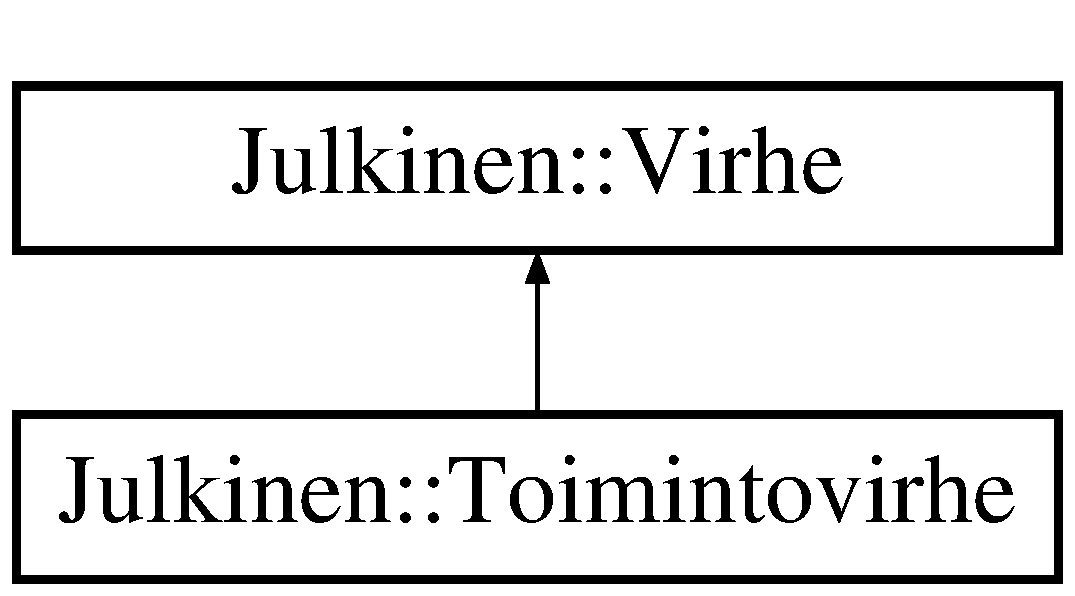
\includegraphics[height=2.000000cm]{class_julkinen_1_1_toimintovirhe}
\end{center}
\end{figure}
\subsection*{Public Types}
\begin{DoxyCompactItemize}
\item 
enum \hyperlink{class_julkinen_1_1_toimintovirhe_a5b3c981a2e64a397ac982787bf310a2c}{Virhekoodi} \{ \\*
\hyperlink{class_julkinen_1_1_toimintovirhe_a5b3c981a2e64a397ac982787bf310a2ca4d1a26345955dbf92b867acd4a5f6e2d}{V\+I\+R\+H\+E\+\_\+\+E\+I\+\_\+\+V\+O\+I\+T\+U\+\_\+\+L\+I\+I\+K\+K\+U\+A\+\_\+\+A\+N\+N\+E\+T\+T\+U\+A\+\_\+\+M\+A\+A\+R\+A\+A}, 
\hyperlink{class_julkinen_1_1_toimintovirhe_a5b3c981a2e64a397ac982787bf310a2ca45456cd1427a07218eccbccf06973be6}{V\+I\+R\+H\+E\+\_\+\+I\+R\+T\+O\+P\+A\+L\+A\+A\+\_\+\+E\+I\+\_\+\+O\+L\+E\+\_\+\+T\+Y\+O\+N\+N\+E\+T\+T\+Y}, 
\hyperlink{class_julkinen_1_1_toimintovirhe_a5b3c981a2e64a397ac982787bf310a2caa4d2e02b06370b32ac15c322ecdfa2df}{V\+I\+R\+H\+E\+\_\+\+I\+R\+T\+O\+P\+A\+L\+A\+A\+\_\+\+O\+N\+\_\+\+J\+O\+\_\+\+T\+Y\+O\+N\+N\+E\+T\+T\+Y}, 
\hyperlink{class_julkinen_1_1_toimintovirhe_a5b3c981a2e64a397ac982787bf310a2ca25224589eb72ebf8375e8b796df90076}{V\+I\+R\+H\+E\+\_\+\+I\+R\+T\+O\+P\+A\+L\+A\+N\+\_\+\+P\+A\+I\+K\+K\+A}, 
\\*
\hyperlink{class_julkinen_1_1_toimintovirhe_a5b3c981a2e64a397ac982787bf310a2caf2e94c361afcf56589dd6f2e0a05857f}{V\+I\+R\+H\+E\+\_\+\+I\+R\+T\+O\+P\+A\+L\+A\+N\+\_\+\+R\+E\+U\+N\+A}, 
\hyperlink{class_julkinen_1_1_toimintovirhe_a5b3c981a2e64a397ac982787bf310a2ca64c902858cd0180525a1b47484b02ada}{V\+I\+R\+H\+E\+\_\+\+I\+R\+T\+O\+P\+A\+L\+A\+N\+\_\+\+R\+O\+T\+A\+A\+T\+I\+O}, 
\hyperlink{class_julkinen_1_1_toimintovirhe_a5b3c981a2e64a397ac982787bf310a2ca6e2d5c8e69dded8f90c7bf8901d72954}{V\+I\+R\+H\+E\+\_\+\+P\+E\+L\+A\+A\+J\+A\+\_\+\+E\+I\+\_\+\+O\+L\+E\+\_\+\+L\+I\+I\+K\+K\+U\+N\+U\+T}, 
\hyperlink{class_julkinen_1_1_toimintovirhe_a5b3c981a2e64a397ac982787bf310a2caf39fe8b019e7a7df69f9b6a79c4c5eea}{V\+I\+R\+H\+E\+\_\+\+P\+E\+L\+A\+A\+J\+A\+\_\+\+O\+N\+\_\+\+J\+O\+\_\+\+L\+I\+I\+K\+K\+U\+N\+U\+T}, 
\\*
\hyperlink{class_julkinen_1_1_toimintovirhe_a5b3c981a2e64a397ac982787bf310a2caa8ac8eac530cd3a661136128f0cc29c9}{V\+I\+R\+H\+E\+\_\+\+L\+I\+I\+K\+K\+E\+E\+N\+\_\+\+S\+U\+U\+N\+T\+A}, 
\hyperlink{class_julkinen_1_1_toimintovirhe_a5b3c981a2e64a397ac982787bf310a2caf41493c1af9268a9664e59acdc200ff5}{V\+I\+R\+H\+E\+\_\+\+T\+U\+N\+N\+I\+S\+T\+A\+M\+A\+T\+O\+N}
 \}\begin{DoxyCompactList}\small\item\em Tunnisteet esimääritellyille virhetilanteille käyttäjän antamissa komennoissa. \end{DoxyCompactList}
\end{DoxyCompactItemize}
\subsection*{Public Member Functions}
\begin{DoxyCompactItemize}
\item 
\hyperlink{class_julkinen_1_1_toimintovirhe_a12dc9116cfc155a3d945f67849d40ba4}{Toimintovirhe} (std\+::string const \&virheviesti)
\begin{DoxyCompactList}\small\item\em Tunnistamaton virhetilanne kopioidulla viestillä. \end{DoxyCompactList}\item 
\hyperlink{class_julkinen_1_1_toimintovirhe_a28d01593d11341bf3fe02963757a6eec}{Toimintovirhe} (\hyperlink{class_julkinen_1_1_toimintovirhe_a5b3c981a2e64a397ac982787bf310a2c}{Virhekoodi} virhekoodi)
\begin{DoxyCompactList}\small\item\em Esimääritelty virhetilanne. \end{DoxyCompactList}\item 
\hyperlink{class_julkinen_1_1_toimintovirhe_a2299cc89c62d178eb4e510b3223b681d}{Toimintovirhe} (\hyperlink{class_julkinen_1_1_toimintovirhe}{Toimintovirhe} const \&toinen)
\begin{DoxyCompactList}\small\item\em Kopiorakentaja. \end{DoxyCompactList}\item 
\hyperlink{class_julkinen_1_1_toimintovirhe_a5b3c981a2e64a397ac982787bf310a2c}{Virhekoodi} \hyperlink{class_julkinen_1_1_toimintovirhe_a4c95cc57f943ee89a4a7cdcbe6236f55}{virhe} () const 
\begin{DoxyCompactList}\small\item\em Sattuneen virhetilanteen virhekoodi. \end{DoxyCompactList}\item 
\hyperlink{class_julkinen_1_1_toimintovirhe}{Toimintovirhe} \& \hyperlink{class_julkinen_1_1_toimintovirhe_aa0db68b7505f9ed596aaa473ef98caf6}{operator=} (\hyperlink{class_julkinen_1_1_toimintovirhe}{Toimintovirhe} const \&toinen)
\begin{DoxyCompactList}\small\item\em Sijoitusoperaattori. \end{DoxyCompactList}\item 
virtual std\+::basic\+\_\+ostream$<$ char $>$ \& \hyperlink{class_julkinen_1_1_toimintovirhe_a6a3078478f0bbf08821d0d5357df2c6a}{tulosta} (std\+::basic\+\_\+ostream$<$ char $>$ \&tuloste) const 
\begin{DoxyCompactList}\small\item\em Tulosta virheen viesti virtaan. \end{DoxyCompactList}\end{DoxyCompactItemize}
\subsection*{Additional Inherited Members}


\subsection{Detailed Description}
Toiminnoissa tapahtuvia virheitä kuvaava poikkeus. 

\subsection{Member Enumeration Documentation}
\hypertarget{class_julkinen_1_1_toimintovirhe_a5b3c981a2e64a397ac982787bf310a2c}{}\index{Julkinen\+::\+Toimintovirhe@{Julkinen\+::\+Toimintovirhe}!Virhekoodi@{Virhekoodi}}
\index{Virhekoodi@{Virhekoodi}!Julkinen\+::\+Toimintovirhe@{Julkinen\+::\+Toimintovirhe}}
\subsubsection[{Virhekoodi}]{\setlength{\rightskip}{0pt plus 5cm}enum {\bf Julkinen\+::\+Toimintovirhe\+::\+Virhekoodi}}\label{class_julkinen_1_1_toimintovirhe_a5b3c981a2e64a397ac982787bf310a2c}


Tunnisteet esimääritellyille virhetilanteille käyttäjän antamissa komennoissa. 

\begin{Desc}
\item[Enumerator]\par
\begin{description}
\index{V\+I\+R\+H\+E\+\_\+\+E\+I\+\_\+\+V\+O\+I\+T\+U\+\_\+\+L\+I\+I\+K\+K\+U\+A\+\_\+\+A\+N\+N\+E\+T\+T\+U\+A\+\_\+\+M\+A\+A\+R\+A\+A@{V\+I\+R\+H\+E\+\_\+\+E\+I\+\_\+\+V\+O\+I\+T\+U\+\_\+\+L\+I\+I\+K\+K\+U\+A\+\_\+\+A\+N\+N\+E\+T\+T\+U\+A\+\_\+\+M\+A\+A\+R\+A\+A}!Julkinen\+::\+Toimintovirhe@{Julkinen\+::\+Toimintovirhe}}\index{Julkinen\+::\+Toimintovirhe@{Julkinen\+::\+Toimintovirhe}!V\+I\+R\+H\+E\+\_\+\+E\+I\+\_\+\+V\+O\+I\+T\+U\+\_\+\+L\+I\+I\+K\+K\+U\+A\+\_\+\+A\+N\+N\+E\+T\+T\+U\+A\+\_\+\+M\+A\+A\+R\+A\+A@{V\+I\+R\+H\+E\+\_\+\+E\+I\+\_\+\+V\+O\+I\+T\+U\+\_\+\+L\+I\+I\+K\+K\+U\+A\+\_\+\+A\+N\+N\+E\+T\+T\+U\+A\+\_\+\+M\+A\+A\+R\+A\+A}}\item[{\em 
\hypertarget{class_julkinen_1_1_toimintovirhe_a5b3c981a2e64a397ac982787bf310a2ca4d1a26345955dbf92b867acd4a5f6e2d}{}V\+I\+R\+H\+E\+\_\+\+E\+I\+\_\+\+V\+O\+I\+T\+U\+\_\+\+L\+I\+I\+K\+K\+U\+A\+\_\+\+A\+N\+N\+E\+T\+T\+U\+A\+\_\+\+M\+A\+A\+R\+A\+A\label{class_julkinen_1_1_toimintovirhe_a5b3c981a2e64a397ac982787bf310a2ca4d1a26345955dbf92b867acd4a5f6e2d}
}]\hyperlink{class_pelaaja}{Pelaaja} ei pysty liikkumaan annetua määrää, annettuun suuntaan. \index{V\+I\+R\+H\+E\+\_\+\+I\+R\+T\+O\+P\+A\+L\+A\+A\+\_\+\+E\+I\+\_\+\+O\+L\+E\+\_\+\+T\+Y\+O\+N\+N\+E\+T\+T\+Y@{V\+I\+R\+H\+E\+\_\+\+I\+R\+T\+O\+P\+A\+L\+A\+A\+\_\+\+E\+I\+\_\+\+O\+L\+E\+\_\+\+T\+Y\+O\+N\+N\+E\+T\+T\+Y}!Julkinen\+::\+Toimintovirhe@{Julkinen\+::\+Toimintovirhe}}\index{Julkinen\+::\+Toimintovirhe@{Julkinen\+::\+Toimintovirhe}!V\+I\+R\+H\+E\+\_\+\+I\+R\+T\+O\+P\+A\+L\+A\+A\+\_\+\+E\+I\+\_\+\+O\+L\+E\+\_\+\+T\+Y\+O\+N\+N\+E\+T\+T\+Y@{V\+I\+R\+H\+E\+\_\+\+I\+R\+T\+O\+P\+A\+L\+A\+A\+\_\+\+E\+I\+\_\+\+O\+L\+E\+\_\+\+T\+Y\+O\+N\+N\+E\+T\+T\+Y}}\item[{\em 
\hypertarget{class_julkinen_1_1_toimintovirhe_a5b3c981a2e64a397ac982787bf310a2ca45456cd1427a07218eccbccf06973be6}{}V\+I\+R\+H\+E\+\_\+\+I\+R\+T\+O\+P\+A\+L\+A\+A\+\_\+\+E\+I\+\_\+\+O\+L\+E\+\_\+\+T\+Y\+O\+N\+N\+E\+T\+T\+Y\label{class_julkinen_1_1_toimintovirhe_a5b3c981a2e64a397ac982787bf310a2ca45456cd1427a07218eccbccf06973be6}
}]\hyperlink{class_pelaaja}{Pelaaja} ei ole työntänyt irtopalaa tällä vuorolla. \index{V\+I\+R\+H\+E\+\_\+\+I\+R\+T\+O\+P\+A\+L\+A\+A\+\_\+\+O\+N\+\_\+\+J\+O\+\_\+\+T\+Y\+O\+N\+N\+E\+T\+T\+Y@{V\+I\+R\+H\+E\+\_\+\+I\+R\+T\+O\+P\+A\+L\+A\+A\+\_\+\+O\+N\+\_\+\+J\+O\+\_\+\+T\+Y\+O\+N\+N\+E\+T\+T\+Y}!Julkinen\+::\+Toimintovirhe@{Julkinen\+::\+Toimintovirhe}}\index{Julkinen\+::\+Toimintovirhe@{Julkinen\+::\+Toimintovirhe}!V\+I\+R\+H\+E\+\_\+\+I\+R\+T\+O\+P\+A\+L\+A\+A\+\_\+\+O\+N\+\_\+\+J\+O\+\_\+\+T\+Y\+O\+N\+N\+E\+T\+T\+Y@{V\+I\+R\+H\+E\+\_\+\+I\+R\+T\+O\+P\+A\+L\+A\+A\+\_\+\+O\+N\+\_\+\+J\+O\+\_\+\+T\+Y\+O\+N\+N\+E\+T\+T\+Y}}\item[{\em 
\hypertarget{class_julkinen_1_1_toimintovirhe_a5b3c981a2e64a397ac982787bf310a2caa4d2e02b06370b32ac15c322ecdfa2df}{}V\+I\+R\+H\+E\+\_\+\+I\+R\+T\+O\+P\+A\+L\+A\+A\+\_\+\+O\+N\+\_\+\+J\+O\+\_\+\+T\+Y\+O\+N\+N\+E\+T\+T\+Y\label{class_julkinen_1_1_toimintovirhe_a5b3c981a2e64a397ac982787bf310a2caa4d2e02b06370b32ac15c322ecdfa2df}
}]\hyperlink{class_pelaaja}{Pelaaja} on jo työntänyt irtopalan tällä vuorolla. \index{V\+I\+R\+H\+E\+\_\+\+I\+R\+T\+O\+P\+A\+L\+A\+N\+\_\+\+P\+A\+I\+K\+K\+A@{V\+I\+R\+H\+E\+\_\+\+I\+R\+T\+O\+P\+A\+L\+A\+N\+\_\+\+P\+A\+I\+K\+K\+A}!Julkinen\+::\+Toimintovirhe@{Julkinen\+::\+Toimintovirhe}}\index{Julkinen\+::\+Toimintovirhe@{Julkinen\+::\+Toimintovirhe}!V\+I\+R\+H\+E\+\_\+\+I\+R\+T\+O\+P\+A\+L\+A\+N\+\_\+\+P\+A\+I\+K\+K\+A@{V\+I\+R\+H\+E\+\_\+\+I\+R\+T\+O\+P\+A\+L\+A\+N\+\_\+\+P\+A\+I\+K\+K\+A}}\item[{\em 
\hypertarget{class_julkinen_1_1_toimintovirhe_a5b3c981a2e64a397ac982787bf310a2ca25224589eb72ebf8375e8b796df90076}{}V\+I\+R\+H\+E\+\_\+\+I\+R\+T\+O\+P\+A\+L\+A\+N\+\_\+\+P\+A\+I\+K\+K\+A\label{class_julkinen_1_1_toimintovirhe_a5b3c981a2e64a397ac982787bf310a2ca25224589eb72ebf8375e8b796df90076}
}]Irtopalan paikka on virheellinen. \index{V\+I\+R\+H\+E\+\_\+\+I\+R\+T\+O\+P\+A\+L\+A\+N\+\_\+\+R\+E\+U\+N\+A@{V\+I\+R\+H\+E\+\_\+\+I\+R\+T\+O\+P\+A\+L\+A\+N\+\_\+\+R\+E\+U\+N\+A}!Julkinen\+::\+Toimintovirhe@{Julkinen\+::\+Toimintovirhe}}\index{Julkinen\+::\+Toimintovirhe@{Julkinen\+::\+Toimintovirhe}!V\+I\+R\+H\+E\+\_\+\+I\+R\+T\+O\+P\+A\+L\+A\+N\+\_\+\+R\+E\+U\+N\+A@{V\+I\+R\+H\+E\+\_\+\+I\+R\+T\+O\+P\+A\+L\+A\+N\+\_\+\+R\+E\+U\+N\+A}}\item[{\em 
\hypertarget{class_julkinen_1_1_toimintovirhe_a5b3c981a2e64a397ac982787bf310a2caf2e94c361afcf56589dd6f2e0a05857f}{}V\+I\+R\+H\+E\+\_\+\+I\+R\+T\+O\+P\+A\+L\+A\+N\+\_\+\+R\+E\+U\+N\+A\label{class_julkinen_1_1_toimintovirhe_a5b3c981a2e64a397ac982787bf310a2caf2e94c361afcf56589dd6f2e0a05857f}
}]Irtopalan reuna on virheellinen. \index{V\+I\+R\+H\+E\+\_\+\+I\+R\+T\+O\+P\+A\+L\+A\+N\+\_\+\+R\+O\+T\+A\+A\+T\+I\+O@{V\+I\+R\+H\+E\+\_\+\+I\+R\+T\+O\+P\+A\+L\+A\+N\+\_\+\+R\+O\+T\+A\+A\+T\+I\+O}!Julkinen\+::\+Toimintovirhe@{Julkinen\+::\+Toimintovirhe}}\index{Julkinen\+::\+Toimintovirhe@{Julkinen\+::\+Toimintovirhe}!V\+I\+R\+H\+E\+\_\+\+I\+R\+T\+O\+P\+A\+L\+A\+N\+\_\+\+R\+O\+T\+A\+A\+T\+I\+O@{V\+I\+R\+H\+E\+\_\+\+I\+R\+T\+O\+P\+A\+L\+A\+N\+\_\+\+R\+O\+T\+A\+A\+T\+I\+O}}\item[{\em 
\hypertarget{class_julkinen_1_1_toimintovirhe_a5b3c981a2e64a397ac982787bf310a2ca64c902858cd0180525a1b47484b02ada}{}V\+I\+R\+H\+E\+\_\+\+I\+R\+T\+O\+P\+A\+L\+A\+N\+\_\+\+R\+O\+T\+A\+A\+T\+I\+O\label{class_julkinen_1_1_toimintovirhe_a5b3c981a2e64a397ac982787bf310a2ca64c902858cd0180525a1b47484b02ada}
}]Irtopalan rotaatio on virheellinen. \index{V\+I\+R\+H\+E\+\_\+\+P\+E\+L\+A\+A\+J\+A\+\_\+\+E\+I\+\_\+\+O\+L\+E\+\_\+\+L\+I\+I\+K\+K\+U\+N\+U\+T@{V\+I\+R\+H\+E\+\_\+\+P\+E\+L\+A\+A\+J\+A\+\_\+\+E\+I\+\_\+\+O\+L\+E\+\_\+\+L\+I\+I\+K\+K\+U\+N\+U\+T}!Julkinen\+::\+Toimintovirhe@{Julkinen\+::\+Toimintovirhe}}\index{Julkinen\+::\+Toimintovirhe@{Julkinen\+::\+Toimintovirhe}!V\+I\+R\+H\+E\+\_\+\+P\+E\+L\+A\+A\+J\+A\+\_\+\+E\+I\+\_\+\+O\+L\+E\+\_\+\+L\+I\+I\+K\+K\+U\+N\+U\+T@{V\+I\+R\+H\+E\+\_\+\+P\+E\+L\+A\+A\+J\+A\+\_\+\+E\+I\+\_\+\+O\+L\+E\+\_\+\+L\+I\+I\+K\+K\+U\+N\+U\+T}}\item[{\em 
\hypertarget{class_julkinen_1_1_toimintovirhe_a5b3c981a2e64a397ac982787bf310a2ca6e2d5c8e69dded8f90c7bf8901d72954}{}V\+I\+R\+H\+E\+\_\+\+P\+E\+L\+A\+A\+J\+A\+\_\+\+E\+I\+\_\+\+O\+L\+E\+\_\+\+L\+I\+I\+K\+K\+U\+N\+U\+T\label{class_julkinen_1_1_toimintovirhe_a5b3c981a2e64a397ac982787bf310a2ca6e2d5c8e69dded8f90c7bf8901d72954}
}]\hyperlink{class_pelaaja}{Pelaaja} ei ole liikkunut tällä vuorolla. \index{V\+I\+R\+H\+E\+\_\+\+P\+E\+L\+A\+A\+J\+A\+\_\+\+O\+N\+\_\+\+J\+O\+\_\+\+L\+I\+I\+K\+K\+U\+N\+U\+T@{V\+I\+R\+H\+E\+\_\+\+P\+E\+L\+A\+A\+J\+A\+\_\+\+O\+N\+\_\+\+J\+O\+\_\+\+L\+I\+I\+K\+K\+U\+N\+U\+T}!Julkinen\+::\+Toimintovirhe@{Julkinen\+::\+Toimintovirhe}}\index{Julkinen\+::\+Toimintovirhe@{Julkinen\+::\+Toimintovirhe}!V\+I\+R\+H\+E\+\_\+\+P\+E\+L\+A\+A\+J\+A\+\_\+\+O\+N\+\_\+\+J\+O\+\_\+\+L\+I\+I\+K\+K\+U\+N\+U\+T@{V\+I\+R\+H\+E\+\_\+\+P\+E\+L\+A\+A\+J\+A\+\_\+\+O\+N\+\_\+\+J\+O\+\_\+\+L\+I\+I\+K\+K\+U\+N\+U\+T}}\item[{\em 
\hypertarget{class_julkinen_1_1_toimintovirhe_a5b3c981a2e64a397ac982787bf310a2caf39fe8b019e7a7df69f9b6a79c4c5eea}{}V\+I\+R\+H\+E\+\_\+\+P\+E\+L\+A\+A\+J\+A\+\_\+\+O\+N\+\_\+\+J\+O\+\_\+\+L\+I\+I\+K\+K\+U\+N\+U\+T\label{class_julkinen_1_1_toimintovirhe_a5b3c981a2e64a397ac982787bf310a2caf39fe8b019e7a7df69f9b6a79c4c5eea}
}]\hyperlink{class_pelaaja}{Pelaaja} on jo liikkunut tällä vuorolla. \index{V\+I\+R\+H\+E\+\_\+\+L\+I\+I\+K\+K\+E\+E\+N\+\_\+\+S\+U\+U\+N\+T\+A@{V\+I\+R\+H\+E\+\_\+\+L\+I\+I\+K\+K\+E\+E\+N\+\_\+\+S\+U\+U\+N\+T\+A}!Julkinen\+::\+Toimintovirhe@{Julkinen\+::\+Toimintovirhe}}\index{Julkinen\+::\+Toimintovirhe@{Julkinen\+::\+Toimintovirhe}!V\+I\+R\+H\+E\+\_\+\+L\+I\+I\+K\+K\+E\+E\+N\+\_\+\+S\+U\+U\+N\+T\+A@{V\+I\+R\+H\+E\+\_\+\+L\+I\+I\+K\+K\+E\+E\+N\+\_\+\+S\+U\+U\+N\+T\+A}}\item[{\em 
\hypertarget{class_julkinen_1_1_toimintovirhe_a5b3c981a2e64a397ac982787bf310a2caa8ac8eac530cd3a661136128f0cc29c9}{}V\+I\+R\+H\+E\+\_\+\+L\+I\+I\+K\+K\+E\+E\+N\+\_\+\+S\+U\+U\+N\+T\+A\label{class_julkinen_1_1_toimintovirhe_a5b3c981a2e64a397ac982787bf310a2caa8ac8eac530cd3a661136128f0cc29c9}
}]Liikeen suunta on virheellinen. \index{V\+I\+R\+H\+E\+\_\+\+T\+U\+N\+N\+I\+S\+T\+A\+M\+A\+T\+O\+N@{V\+I\+R\+H\+E\+\_\+\+T\+U\+N\+N\+I\+S\+T\+A\+M\+A\+T\+O\+N}!Julkinen\+::\+Toimintovirhe@{Julkinen\+::\+Toimintovirhe}}\index{Julkinen\+::\+Toimintovirhe@{Julkinen\+::\+Toimintovirhe}!V\+I\+R\+H\+E\+\_\+\+T\+U\+N\+N\+I\+S\+T\+A\+M\+A\+T\+O\+N@{V\+I\+R\+H\+E\+\_\+\+T\+U\+N\+N\+I\+S\+T\+A\+M\+A\+T\+O\+N}}\item[{\em 
\hypertarget{class_julkinen_1_1_toimintovirhe_a5b3c981a2e64a397ac982787bf310a2caf41493c1af9268a9664e59acdc200ff5}{}V\+I\+R\+H\+E\+\_\+\+T\+U\+N\+N\+I\+S\+T\+A\+M\+A\+T\+O\+N\label{class_julkinen_1_1_toimintovirhe_a5b3c981a2e64a397ac982787bf310a2caf41493c1af9268a9664e59acdc200ff5}
}]Tunnistamaton virhe. \end{description}
\end{Desc}


\subsection{Constructor \& Destructor Documentation}
\hypertarget{class_julkinen_1_1_toimintovirhe_a12dc9116cfc155a3d945f67849d40ba4}{}\index{Julkinen\+::\+Toimintovirhe@{Julkinen\+::\+Toimintovirhe}!Toimintovirhe@{Toimintovirhe}}
\index{Toimintovirhe@{Toimintovirhe}!Julkinen\+::\+Toimintovirhe@{Julkinen\+::\+Toimintovirhe}}
\subsubsection[{Toimintovirhe(std\+::string const \&virheviesti)}]{\setlength{\rightskip}{0pt plus 5cm}Toimintovirhe\+::\+Toimintovirhe (
\begin{DoxyParamCaption}
\item[{std\+::string const \&}]{virheviesti}
\end{DoxyParamCaption}
)\hspace{0.3cm}{\ttfamily [explicit]}}\label{class_julkinen_1_1_toimintovirhe_a12dc9116cfc155a3d945f67849d40ba4}


Tunnistamaton virhetilanne kopioidulla viestillä. 

Käytä tätä vain, jos kyseessä ei ole mikään esimääritellyistä virheistä.

\begin{DoxyPostcond}{Postcondition}
Perustakuu poikkeuksen sattuessa. 
\end{DoxyPostcond}

\begin{DoxyParams}{Parameters}
{\em virheviesti} & Merkkijono, joka kopioidaan poikkeuksen viestiksi. \\
\hline
\end{DoxyParams}

\begin{DoxyExceptions}{Exceptions}
{\em std\+::bad\+\_\+alloc} & Ei saatu varattua muistia viestiä varten. \\
\hline
\end{DoxyExceptions}
\hypertarget{class_julkinen_1_1_toimintovirhe_a28d01593d11341bf3fe02963757a6eec}{}\index{Julkinen\+::\+Toimintovirhe@{Julkinen\+::\+Toimintovirhe}!Toimintovirhe@{Toimintovirhe}}
\index{Toimintovirhe@{Toimintovirhe}!Julkinen\+::\+Toimintovirhe@{Julkinen\+::\+Toimintovirhe}}
\subsubsection[{Toimintovirhe(\+Virhekoodi virhekoodi)}]{\setlength{\rightskip}{0pt plus 5cm}Toimintovirhe\+::\+Toimintovirhe (
\begin{DoxyParamCaption}
\item[{{\bf Virhekoodi}}]{virhekoodi}
\end{DoxyParamCaption}
)\hspace{0.3cm}{\ttfamily [explicit]}}\label{class_julkinen_1_1_toimintovirhe_a28d01593d11341bf3fe02963757a6eec}


Esimääritelty virhetilanne. 

\begin{DoxyPostcond}{Postcondition}
No-\/throw -\/takuu. 
\end{DoxyPostcond}

\begin{DoxyParams}{Parameters}
{\em virhekoodi} & Virhetilanteen tunniste. Mikäli koodi on V\+I\+R\+H\+E\+\_\+\+T\+U\+N\+N\+I\+S\+T\+A\+M\+A\+T\+O\+N, tulee viestiksi \char`\"{}\+Tunnistamaton virhe.\char`\"{}. \\
\hline
\end{DoxyParams}
\hypertarget{class_julkinen_1_1_toimintovirhe_a2299cc89c62d178eb4e510b3223b681d}{}\index{Julkinen\+::\+Toimintovirhe@{Julkinen\+::\+Toimintovirhe}!Toimintovirhe@{Toimintovirhe}}
\index{Toimintovirhe@{Toimintovirhe}!Julkinen\+::\+Toimintovirhe@{Julkinen\+::\+Toimintovirhe}}
\subsubsection[{Toimintovirhe(\+Toimintovirhe const \&toinen)}]{\setlength{\rightskip}{0pt plus 5cm}Toimintovirhe\+::\+Toimintovirhe (
\begin{DoxyParamCaption}
\item[{{\bf Toimintovirhe} const \&}]{toinen}
\end{DoxyParamCaption}
)}\label{class_julkinen_1_1_toimintovirhe_a2299cc89c62d178eb4e510b3223b681d}


Kopiorakentaja. 

\begin{DoxyPostcond}{Postcondition}
No-\/throw -\/takuu. 
\end{DoxyPostcond}


\subsection{Member Function Documentation}
\hypertarget{class_julkinen_1_1_toimintovirhe_aa0db68b7505f9ed596aaa473ef98caf6}{}\index{Julkinen\+::\+Toimintovirhe@{Julkinen\+::\+Toimintovirhe}!operator=@{operator=}}
\index{operator=@{operator=}!Julkinen\+::\+Toimintovirhe@{Julkinen\+::\+Toimintovirhe}}
\subsubsection[{operator=(\+Toimintovirhe const \&toinen)}]{\setlength{\rightskip}{0pt plus 5cm}{\bf Toimintovirhe} \& Toimintovirhe\+::operator= (
\begin{DoxyParamCaption}
\item[{{\bf Toimintovirhe} const \&}]{toinen}
\end{DoxyParamCaption}
)}\label{class_julkinen_1_1_toimintovirhe_aa0db68b7505f9ed596aaa473ef98caf6}


Sijoitusoperaattori. 

\begin{DoxyPostcond}{Postcondition}
No-\/throw -\/takuu. 
\end{DoxyPostcond}
\hypertarget{class_julkinen_1_1_toimintovirhe_a6a3078478f0bbf08821d0d5357df2c6a}{}\index{Julkinen\+::\+Toimintovirhe@{Julkinen\+::\+Toimintovirhe}!tulosta@{tulosta}}
\index{tulosta@{tulosta}!Julkinen\+::\+Toimintovirhe@{Julkinen\+::\+Toimintovirhe}}
\subsubsection[{tulosta(std\+::basic\+\_\+ostream$<$ char $>$ \&tuloste) const }]{\setlength{\rightskip}{0pt plus 5cm}basic\+\_\+ostream$<$ char $>$ \& Toimintovirhe\+::tulosta (
\begin{DoxyParamCaption}
\item[{std\+::basic\+\_\+ostream$<$ char $>$ \&}]{tuloste}
\end{DoxyParamCaption}
) const\hspace{0.3cm}{\ttfamily [virtual]}}\label{class_julkinen_1_1_toimintovirhe_a6a3078478f0bbf08821d0d5357df2c6a}


Tulosta virheen viesti virtaan. 

Tulostaa virheen viestin virtaan, eikä tee muuta.

\begin{DoxyPostcond}{Postcondition}
Vahva poikkeustakuu. 
\end{DoxyPostcond}

\begin{DoxyParams}{Parameters}
{\em tuloste} & Virta, jonne viesti tulostetaan. \\
\hline
\end{DoxyParams}
\begin{DoxyReturn}{Returns}
{\ttfamily tuloste} 
\end{DoxyReturn}


Reimplemented from \hyperlink{class_julkinen_1_1_virhe_a36a2644943038f9760b5d76a1960b00d}{Julkinen\+::\+Virhe}.

\hypertarget{class_julkinen_1_1_toimintovirhe_a4c95cc57f943ee89a4a7cdcbe6236f55}{}\index{Julkinen\+::\+Toimintovirhe@{Julkinen\+::\+Toimintovirhe}!virhe@{virhe}}
\index{virhe@{virhe}!Julkinen\+::\+Toimintovirhe@{Julkinen\+::\+Toimintovirhe}}
\subsubsection[{virhe() const }]{\setlength{\rightskip}{0pt plus 5cm}{\bf Toimintovirhe\+::\+Virhekoodi} Toimintovirhe\+::virhe (
\begin{DoxyParamCaption}
{}
\end{DoxyParamCaption}
) const}\label{class_julkinen_1_1_toimintovirhe_a4c95cc57f943ee89a4a7cdcbe6236f55}


Sattuneen virhetilanteen virhekoodi. 

\begin{DoxyReturn}{Returns}
Palauttaa virheen {\ttfamily Virhekoodi}. 
\end{DoxyReturn}


The documentation for this class was generated from the following files\+:\begin{DoxyCompactItemize}
\item 
\hyperlink{toimintovirhe_8hh}{toimintovirhe.\+hh}\item 
valmiiden\+\_\+toteutus/\hyperlink{toimintovirhe_8cc}{toimintovirhe.\+cc}\end{DoxyCompactItemize}

\hypertarget{class_julkinen_1_1_toteuttamaton_virhe}{}\section{Julkinen\+:\+:Toteuttamaton\+Virhe Class Reference}
\label{class_julkinen_1_1_toteuttamaton_virhe}\index{Julkinen\+::\+Toteuttamaton\+Virhe@{Julkinen\+::\+Toteuttamaton\+Virhe}}


Toimintoa ei ole vielä toteutettu.  




{\ttfamily \#include $<$toteuttamaton\+\_\+virhe.\+hh$>$}

Inheritance diagram for Julkinen\+:\+:Toteuttamaton\+Virhe\+:\begin{figure}[H]
\begin{center}
\leavevmode
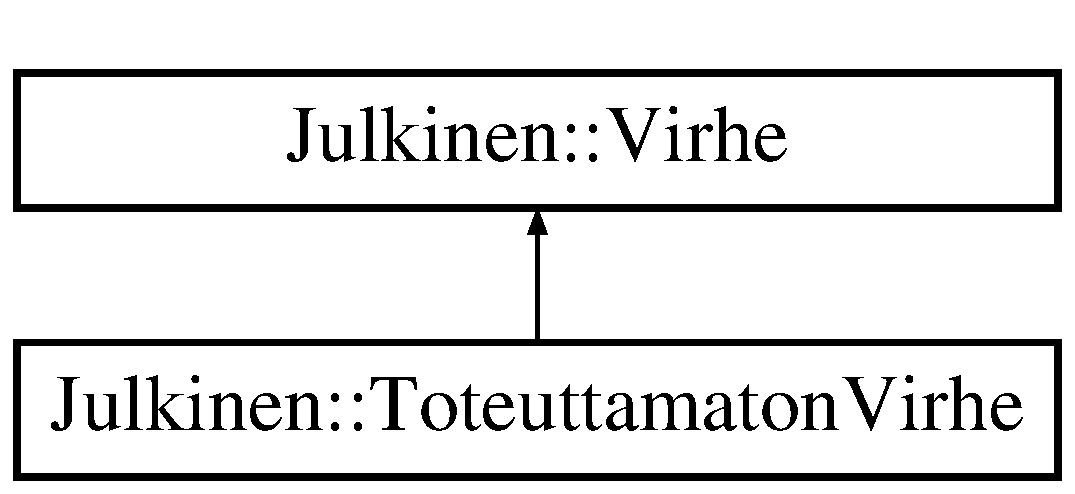
\includegraphics[height=2.000000cm]{class_julkinen_1_1_toteuttamaton_virhe}
\end{center}
\end{figure}
\subsection*{Public Member Functions}
\begin{DoxyCompactItemize}
\item 
\hyperlink{class_julkinen_1_1_toteuttamaton_virhe_a99a4a348aae94e693dd7f00e1972a5d5}{Toteuttamaton\+Virhe} (std\+::string const \&virheviesti)
\begin{DoxyCompactList}\small\item\em Kopioidulla viestillä. \end{DoxyCompactList}\item 
\hyperlink{class_julkinen_1_1_toteuttamaton_virhe_a202f4895091f54a386b180a948e60340}{Toteuttamaton\+Virhe} (const char $\ast$virheviesti)
\begin{DoxyCompactList}\small\item\em Muualla tallessa olevalla viestillä. \end{DoxyCompactList}\item 
\hyperlink{class_julkinen_1_1_toteuttamaton_virhe_a66deecd233993b61cfa7a72952235872}{Toteuttamaton\+Virhe} (\hyperlink{class_julkinen_1_1_toteuttamaton_virhe}{Toteuttamaton\+Virhe} const \&toinen)
\begin{DoxyCompactList}\small\item\em Kopiorakentaja. \end{DoxyCompactList}\item 
virtual \hyperlink{class_julkinen_1_1_toteuttamaton_virhe_a433af1932c8db53951d2d360a3fe4fab}{$\sim$\+Toteuttamaton\+Virhe} ()
\begin{DoxyCompactList}\small\item\em Purkaja. \end{DoxyCompactList}\item 
\hyperlink{class_julkinen_1_1_toteuttamaton_virhe}{Toteuttamaton\+Virhe} \& \hyperlink{class_julkinen_1_1_toteuttamaton_virhe_a35e5217128b97768e4bbccea860362f1}{operator=} (\hyperlink{class_julkinen_1_1_toteuttamaton_virhe}{Toteuttamaton\+Virhe} const \&toinen)
\begin{DoxyCompactList}\small\item\em Sijoitusoperaattori. \end{DoxyCompactList}\end{DoxyCompactItemize}
\subsection*{Additional Inherited Members}


\subsection{Detailed Description}
Toimintoa ei ole vielä toteutettu. 

Mikäli rajapinnan toteuttavassa luokassa on tynkätoteutuksia, joiden ei kuulukaan vielä toimia, niiden tulee heittää tätä tyyppiä oleva poikkeus. 

\subsection{Constructor \& Destructor Documentation}
\hypertarget{class_julkinen_1_1_toteuttamaton_virhe_a99a4a348aae94e693dd7f00e1972a5d5}{}\index{Julkinen\+::\+Toteuttamaton\+Virhe@{Julkinen\+::\+Toteuttamaton\+Virhe}!Toteuttamaton\+Virhe@{Toteuttamaton\+Virhe}}
\index{Toteuttamaton\+Virhe@{Toteuttamaton\+Virhe}!Julkinen\+::\+Toteuttamaton\+Virhe@{Julkinen\+::\+Toteuttamaton\+Virhe}}
\subsubsection[{Toteuttamaton\+Virhe(std\+::string const \&virheviesti)}]{\setlength{\rightskip}{0pt plus 5cm}Toteuttamaton\+Virhe\+::\+Toteuttamaton\+Virhe (
\begin{DoxyParamCaption}
\item[{std\+::string const \&}]{virheviesti}
\end{DoxyParamCaption}
)\hspace{0.3cm}{\ttfamily [explicit]}}\label{class_julkinen_1_1_toteuttamaton_virhe_a99a4a348aae94e693dd7f00e1972a5d5}


Kopioidulla viestillä. 

\begin{DoxyPostcond}{Postcondition}
Perustakuu poikkeuksen sattuessa. 
\end{DoxyPostcond}

\begin{DoxyParams}{Parameters}
{\em virheviesti} & Merkkijono, joka kopioidaan poikkeuksen viestiksi. \\
\hline
\end{DoxyParams}

\begin{DoxyExceptions}{Exceptions}
{\em std\+::bad\+\_\+alloc} & Ei saatu varattua muistia viestiä varten. \\
\hline
\end{DoxyExceptions}
\hypertarget{class_julkinen_1_1_toteuttamaton_virhe_a202f4895091f54a386b180a948e60340}{}\index{Julkinen\+::\+Toteuttamaton\+Virhe@{Julkinen\+::\+Toteuttamaton\+Virhe}!Toteuttamaton\+Virhe@{Toteuttamaton\+Virhe}}
\index{Toteuttamaton\+Virhe@{Toteuttamaton\+Virhe}!Julkinen\+::\+Toteuttamaton\+Virhe@{Julkinen\+::\+Toteuttamaton\+Virhe}}
\subsubsection[{Toteuttamaton\+Virhe(const char $\ast$virheviesti)}]{\setlength{\rightskip}{0pt plus 5cm}Toteuttamaton\+Virhe\+::\+Toteuttamaton\+Virhe (
\begin{DoxyParamCaption}
\item[{const char $\ast$}]{virheviesti}
\end{DoxyParamCaption}
)\hspace{0.3cm}{\ttfamily [explicit]}}\label{class_julkinen_1_1_toteuttamaton_virhe_a202f4895091f54a386b180a948e60340}


Muualla tallessa olevalla viestillä. 

H\+U\+O\+M! Tämä luokka {\itshape ei} ota vastuuta osoittimen päässä olevan olion tuhoamisesta, eikä tee osoittimen osoittamasta tiedosta kopiota. Tarkoituksena on antaa osoitin esim. käännösyksikön tai luokan sisäiseen virheviestivakioon, jotta tämä rakentaja voi tarjota no-\/throw -\/takuun.

\begin{DoxyPostcond}{Postcondition}
No-\/throw -\/takuu. 
\end{DoxyPostcond}

\begin{DoxyParams}[1]{Parameters}
\mbox{\tt in}  & {\em virheviesti} & Osoitin oikeaan C-\/merkkijonovakioon tai vakioisen {\ttfamily std\+::string}-\/olion {\ttfamily c\+\_\+str()} metodin palauttamaan arvoon. \\
\hline
\end{DoxyParams}
\hypertarget{class_julkinen_1_1_toteuttamaton_virhe_a66deecd233993b61cfa7a72952235872}{}\index{Julkinen\+::\+Toteuttamaton\+Virhe@{Julkinen\+::\+Toteuttamaton\+Virhe}!Toteuttamaton\+Virhe@{Toteuttamaton\+Virhe}}
\index{Toteuttamaton\+Virhe@{Toteuttamaton\+Virhe}!Julkinen\+::\+Toteuttamaton\+Virhe@{Julkinen\+::\+Toteuttamaton\+Virhe}}
\subsubsection[{Toteuttamaton\+Virhe(\+Toteuttamaton\+Virhe const \&toinen)}]{\setlength{\rightskip}{0pt plus 5cm}Toteuttamaton\+Virhe\+::\+Toteuttamaton\+Virhe (
\begin{DoxyParamCaption}
\item[{{\bf Toteuttamaton\+Virhe} const \&}]{toinen}
\end{DoxyParamCaption}
)}\label{class_julkinen_1_1_toteuttamaton_virhe_a66deecd233993b61cfa7a72952235872}


Kopiorakentaja. 

\begin{DoxyPostcond}{Postcondition}
No-\/throw -\/takuu.
\end{DoxyPostcond}

\begin{DoxyParams}[1]{Parameters}
\mbox{\tt in}  & {\em toinen} & Kopioitava {\ttfamily \hyperlink{class_julkinen_1_1_virhe}{Virhe}}. \\
\hline
\end{DoxyParams}
\hypertarget{class_julkinen_1_1_toteuttamaton_virhe_a433af1932c8db53951d2d360a3fe4fab}{}\index{Julkinen\+::\+Toteuttamaton\+Virhe@{Julkinen\+::\+Toteuttamaton\+Virhe}!````~Toteuttamaton\+Virhe@{$\sim$\+Toteuttamaton\+Virhe}}
\index{````~Toteuttamaton\+Virhe@{$\sim$\+Toteuttamaton\+Virhe}!Julkinen\+::\+Toteuttamaton\+Virhe@{Julkinen\+::\+Toteuttamaton\+Virhe}}
\subsubsection[{$\sim$\+Toteuttamaton\+Virhe()}]{\setlength{\rightskip}{0pt plus 5cm}Toteuttamaton\+Virhe\+::$\sim$\+Toteuttamaton\+Virhe (
\begin{DoxyParamCaption}
{}
\end{DoxyParamCaption}
)\hspace{0.3cm}{\ttfamily [virtual]}}\label{class_julkinen_1_1_toteuttamaton_virhe_a433af1932c8db53951d2d360a3fe4fab}


Purkaja. 

\begin{DoxyPostcond}{Postcondition}
No-\/throw -\/takuu. 
\end{DoxyPostcond}


\subsection{Member Function Documentation}
\hypertarget{class_julkinen_1_1_toteuttamaton_virhe_a35e5217128b97768e4bbccea860362f1}{}\index{Julkinen\+::\+Toteuttamaton\+Virhe@{Julkinen\+::\+Toteuttamaton\+Virhe}!operator=@{operator=}}
\index{operator=@{operator=}!Julkinen\+::\+Toteuttamaton\+Virhe@{Julkinen\+::\+Toteuttamaton\+Virhe}}
\subsubsection[{operator=(\+Toteuttamaton\+Virhe const \&toinen)}]{\setlength{\rightskip}{0pt plus 5cm}{\bf Toteuttamaton\+Virhe} \& Toteuttamaton\+Virhe\+::operator= (
\begin{DoxyParamCaption}
\item[{{\bf Toteuttamaton\+Virhe} const \&}]{toinen}
\end{DoxyParamCaption}
)}\label{class_julkinen_1_1_toteuttamaton_virhe_a35e5217128b97768e4bbccea860362f1}


Sijoitusoperaattori. 

\begin{DoxyPostcond}{Postcondition}
No-\/throw -\/takuu.
\end{DoxyPostcond}

\begin{DoxyParams}[1]{Parameters}
\mbox{\tt in}  & {\em toinen} & Sijoitettava {\ttfamily \hyperlink{class_julkinen_1_1_virhe}{Virhe}}. \\
\hline
\end{DoxyParams}


The documentation for this class was generated from the following files\+:\begin{DoxyCompactItemize}
\item 
\hyperlink{toteuttamaton__virhe_8hh}{toteuttamaton\+\_\+virhe.\+hh}\item 
valmiiden\+\_\+toteutus/\hyperlink{toteuttamaton__virhe_8cc}{toteuttamaton\+\_\+virhe.\+cc}\end{DoxyCompactItemize}

\hypertarget{class_julkinen_1_1_vaittamavirhe}{}\section{Julkinen\+:\+:Vaittamavirhe Class Reference}
\label{class_julkinen_1_1_vaittamavirhe}\index{Julkinen\+::\+Vaittamavirhe@{Julkinen\+::\+Vaittamavirhe}}


Assertio rajapinnan käyttämä virhetyyppi.  




{\ttfamily \#include $<$vaittamavirhe.\+hh$>$}

Inheritance diagram for Julkinen\+:\+:Vaittamavirhe\+:\begin{figure}[H]
\begin{center}
\leavevmode
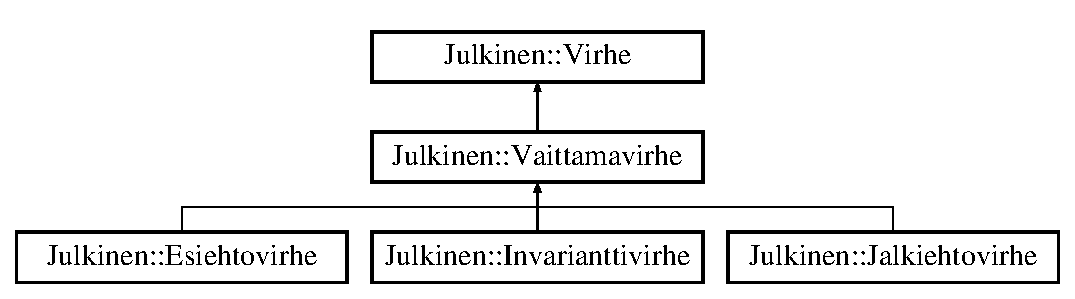
\includegraphics[height=3.000000cm]{class_julkinen_1_1_vaittamavirhe}
\end{center}
\end{figure}
\subsection*{Public Member Functions}
\begin{DoxyCompactItemize}
\item 
\hyperlink{class_julkinen_1_1_vaittamavirhe_a7c6e81b7fdab0248569dc4f68c056361}{Vaittamavirhe} (char const $\ast$lauseke, char const $\ast$\hyperlink{class_julkinen_1_1_vaittamavirhe_a8624cd880b8466188ef6de480431dffb}{tiedosto}, unsigned int \hyperlink{class_julkinen_1_1_vaittamavirhe_abc571141231b3fa789ae41d2d80642ef}{rivi}, char const $\ast$\hyperlink{class_julkinen_1_1_vaittamavirhe_afd5de6b5639336288d28fd077c84a20c}{funktio})  throw ()
\begin{DoxyCompactList}\small\item\em \hyperlink{class_julkinen_1_1_vaittamavirhe}{Vaittamavirhe} rakentaja. \end{DoxyCompactList}\item 
\hyperlink{class_julkinen_1_1_vaittamavirhe_aeea3649f8099e62d6b3dfce35be555be}{Vaittamavirhe} (\hyperlink{class_julkinen_1_1_vaittamavirhe}{Vaittamavirhe} const \&toinen)  throw ()
\begin{DoxyCompactList}\small\item\em Kopiorakentaja. \end{DoxyCompactList}\item 
\hypertarget{class_julkinen_1_1_vaittamavirhe_a410a444f63066447821e76f2d54a23e2}{}virtual \hyperlink{class_julkinen_1_1_vaittamavirhe_a410a444f63066447821e76f2d54a23e2}{$\sim$\+Vaittamavirhe} ()=0  throw ()\label{class_julkinen_1_1_vaittamavirhe_a410a444f63066447821e76f2d54a23e2}

\begin{DoxyCompactList}\small\item\em Purkaja. \end{DoxyCompactList}\item 
char const $\ast$ \hyperlink{class_julkinen_1_1_vaittamavirhe_a8624cd880b8466188ef6de480431dffb}{tiedosto} () const   throw ()
\begin{DoxyCompactList}\small\item\em \hyperlink{class_julkinen_1_1_virhe}{Virhe} tiedoston kertova metodi. \end{DoxyCompactList}\item 
unsigned int \hyperlink{class_julkinen_1_1_vaittamavirhe_abc571141231b3fa789ae41d2d80642ef}{rivi} () const   throw ()
\begin{DoxyCompactList}\small\item\em \hyperlink{class_julkinen_1_1_virhe}{Virhe} rivin kertova metodi. \end{DoxyCompactList}\item 
char const $\ast$ \hyperlink{class_julkinen_1_1_vaittamavirhe_afd5de6b5639336288d28fd077c84a20c}{funktio} () const   throw ()
\begin{DoxyCompactList}\small\item\em \hyperlink{class_julkinen_1_1_virhe}{Virhe} funktion kertova metodi. \end{DoxyCompactList}\item 
std\+::basic\+\_\+ostream$<$ char $>$ \& \hyperlink{class_julkinen_1_1_vaittamavirhe_a5ca289035ecde35b1b1576d1c9219acd}{tulosta} (std\+::basic\+\_\+ostream$<$ char $>$ \&tuloste) const 
\begin{DoxyCompactList}\small\item\em Tulostus virran luonti metodi. \end{DoxyCompactList}\item 
\hyperlink{class_julkinen_1_1_vaittamavirhe}{Vaittamavirhe} \& \hyperlink{class_julkinen_1_1_vaittamavirhe_a182a03c5e807a02c1ac32a5474f34821}{operator==} (\hyperlink{class_julkinen_1_1_vaittamavirhe}{Vaittamavirhe} const \&toinen)  throw ()
\begin{DoxyCompactList}\small\item\em Yhtäsuuruus vertailu operaattori. \end{DoxyCompactList}\end{DoxyCompactItemize}
\subsection*{Additional Inherited Members}


\subsection{Detailed Description}
Assertio rajapinnan käyttämä virhetyyppi. 

\subsection{Constructor \& Destructor Documentation}
\hypertarget{class_julkinen_1_1_vaittamavirhe_a7c6e81b7fdab0248569dc4f68c056361}{}\index{Julkinen\+::\+Vaittamavirhe@{Julkinen\+::\+Vaittamavirhe}!Vaittamavirhe@{Vaittamavirhe}}
\index{Vaittamavirhe@{Vaittamavirhe}!Julkinen\+::\+Vaittamavirhe@{Julkinen\+::\+Vaittamavirhe}}
\subsubsection[{Vaittamavirhe(char const $\ast$lauseke, char const $\ast$tiedosto, unsigned int rivi, char const $\ast$funktio)}]{\setlength{\rightskip}{0pt plus 5cm}Vaittamavirhe\+::\+Vaittamavirhe (
\begin{DoxyParamCaption}
\item[{char const $\ast$}]{lauseke, }
\item[{char const $\ast$}]{tiedosto, }
\item[{unsigned int}]{rivi, }
\item[{char const $\ast$}]{funktio}
\end{DoxyParamCaption}
) throw  ) }\label{class_julkinen_1_1_vaittamavirhe_a7c6e81b7fdab0248569dc4f68c056361}


\hyperlink{class_julkinen_1_1_vaittamavirhe}{Vaittamavirhe} rakentaja. 


\begin{DoxyParams}{Parameters}
{\em lauseke} & Merkkijono. \\
\hline
{\em tiedosto} & Merkkijono. \\
\hline
{\em rivi} & Rivinumero. \\
\hline
{\em funktio} & Merkkijono. \\
\hline
\end{DoxyParams}
\hypertarget{class_julkinen_1_1_vaittamavirhe_aeea3649f8099e62d6b3dfce35be555be}{}\index{Julkinen\+::\+Vaittamavirhe@{Julkinen\+::\+Vaittamavirhe}!Vaittamavirhe@{Vaittamavirhe}}
\index{Vaittamavirhe@{Vaittamavirhe}!Julkinen\+::\+Vaittamavirhe@{Julkinen\+::\+Vaittamavirhe}}
\subsubsection[{Vaittamavirhe(\+Vaittamavirhe const \&toinen)}]{\setlength{\rightskip}{0pt plus 5cm}Vaittamavirhe\+::\+Vaittamavirhe (
\begin{DoxyParamCaption}
\item[{{\bf Vaittamavirhe} const \&}]{toinen}
\end{DoxyParamCaption}
) throw  ) }\label{class_julkinen_1_1_vaittamavirhe_aeea3649f8099e62d6b3dfce35be555be}


Kopiorakentaja. 


\begin{DoxyParams}{Parameters}
{\em toinen} & Kopioitava \hyperlink{class_julkinen_1_1_vaittamavirhe}{Vaittamavirhe}. \\
\hline
\end{DoxyParams}


\subsection{Member Function Documentation}
\hypertarget{class_julkinen_1_1_vaittamavirhe_afd5de6b5639336288d28fd077c84a20c}{}\index{Julkinen\+::\+Vaittamavirhe@{Julkinen\+::\+Vaittamavirhe}!funktio@{funktio}}
\index{funktio@{funktio}!Julkinen\+::\+Vaittamavirhe@{Julkinen\+::\+Vaittamavirhe}}
\subsubsection[{funktio() const }]{\setlength{\rightskip}{0pt plus 5cm}char const $\ast$ Vaittamavirhe\+::funktio (
\begin{DoxyParamCaption}
{}
\end{DoxyParamCaption}
) const throw  ) }\label{class_julkinen_1_1_vaittamavirhe_afd5de6b5639336288d28fd077c84a20c}


\hyperlink{class_julkinen_1_1_virhe}{Virhe} funktion kertova metodi. 

\begin{DoxyReturn}{Returns}
Palauttaa virhe funktion nimen. 
\end{DoxyReturn}
\hypertarget{class_julkinen_1_1_vaittamavirhe_a182a03c5e807a02c1ac32a5474f34821}{}\index{Julkinen\+::\+Vaittamavirhe@{Julkinen\+::\+Vaittamavirhe}!operator==@{operator==}}
\index{operator==@{operator==}!Julkinen\+::\+Vaittamavirhe@{Julkinen\+::\+Vaittamavirhe}}
\subsubsection[{operator==(\+Vaittamavirhe const \&toinen)}]{\setlength{\rightskip}{0pt plus 5cm}{\bf Vaittamavirhe} \& Vaittamavirhe\+::operator== (
\begin{DoxyParamCaption}
\item[{{\bf Vaittamavirhe} const \&}]{toinen}
\end{DoxyParamCaption}
) throw  ) }\label{class_julkinen_1_1_vaittamavirhe_a182a03c5e807a02c1ac32a5474f34821}


Yhtäsuuruus vertailu operaattori. 


\begin{DoxyParams}{Parameters}
{\em toinen} & Verrattava \hyperlink{class_julkinen_1_1_vaittamavirhe}{Vaittamavirhe}. \\
\hline
\end{DoxyParams}
\hypertarget{class_julkinen_1_1_vaittamavirhe_abc571141231b3fa789ae41d2d80642ef}{}\index{Julkinen\+::\+Vaittamavirhe@{Julkinen\+::\+Vaittamavirhe}!rivi@{rivi}}
\index{rivi@{rivi}!Julkinen\+::\+Vaittamavirhe@{Julkinen\+::\+Vaittamavirhe}}
\subsubsection[{rivi() const }]{\setlength{\rightskip}{0pt plus 5cm}unsigned int Vaittamavirhe\+::rivi (
\begin{DoxyParamCaption}
{}
\end{DoxyParamCaption}
) const throw  ) }\label{class_julkinen_1_1_vaittamavirhe_abc571141231b3fa789ae41d2d80642ef}


\hyperlink{class_julkinen_1_1_virhe}{Virhe} rivin kertova metodi. 

\begin{DoxyReturn}{Returns}
Palauttaa virheen rivin. 
\end{DoxyReturn}
\hypertarget{class_julkinen_1_1_vaittamavirhe_a8624cd880b8466188ef6de480431dffb}{}\index{Julkinen\+::\+Vaittamavirhe@{Julkinen\+::\+Vaittamavirhe}!tiedosto@{tiedosto}}
\index{tiedosto@{tiedosto}!Julkinen\+::\+Vaittamavirhe@{Julkinen\+::\+Vaittamavirhe}}
\subsubsection[{tiedosto() const }]{\setlength{\rightskip}{0pt plus 5cm}char const $\ast$ Vaittamavirhe\+::tiedosto (
\begin{DoxyParamCaption}
{}
\end{DoxyParamCaption}
) const throw  ) }\label{class_julkinen_1_1_vaittamavirhe_a8624cd880b8466188ef6de480431dffb}


\hyperlink{class_julkinen_1_1_virhe}{Virhe} tiedoston kertova metodi. 

\begin{DoxyReturn}{Returns}
Palauttaa virhe tiedoston nimen. 
\end{DoxyReturn}
\hypertarget{class_julkinen_1_1_vaittamavirhe_a5ca289035ecde35b1b1576d1c9219acd}{}\index{Julkinen\+::\+Vaittamavirhe@{Julkinen\+::\+Vaittamavirhe}!tulosta@{tulosta}}
\index{tulosta@{tulosta}!Julkinen\+::\+Vaittamavirhe@{Julkinen\+::\+Vaittamavirhe}}
\subsubsection[{tulosta(std\+::basic\+\_\+ostream$<$ char $>$ \&tuloste) const }]{\setlength{\rightskip}{0pt plus 5cm}basic\+\_\+ostream$<$ char $>$ \& Vaittamavirhe\+::tulosta (
\begin{DoxyParamCaption}
\item[{std\+::basic\+\_\+ostream$<$ char $>$ \&}]{tuloste}
\end{DoxyParamCaption}
) const\hspace{0.3cm}{\ttfamily [virtual]}}\label{class_julkinen_1_1_vaittamavirhe_a5ca289035ecde35b1b1576d1c9219acd}


Tulostus virran luonti metodi. 


\begin{DoxyParams}{Parameters}
{\em tuloste} & Perus tulostevirta. \\
\hline
\end{DoxyParams}
\begin{DoxyReturn}{Returns}
Palauttaa perus tulostevirran. 
\end{DoxyReturn}


Reimplemented from \hyperlink{class_julkinen_1_1_virhe_a36a2644943038f9760b5d76a1960b00d}{Julkinen\+::\+Virhe}.



The documentation for this class was generated from the following files\+:\begin{DoxyCompactItemize}
\item 
valmiiden\+\_\+toteutus/include/\hyperlink{vaittamavirhe_8hh}{vaittamavirhe.\+hh}\item 
valmiiden\+\_\+toteutus/\hyperlink{vaittamavirhe_8cc}{vaittamavirhe.\+cc}\end{DoxyCompactItemize}

\hypertarget{class_julkinen_1_1_virhe}{}\section{Julkinen\+:\+:Virhe Class Reference}
\label{class_julkinen_1_1_virhe}\index{Julkinen\+::\+Virhe@{Julkinen\+::\+Virhe}}


Labyrintin poikkeusten kantaluokka.  




{\ttfamily \#include $<$virhe.\+hh$>$}

Inheritance diagram for Julkinen\+:\+:Virhe\+:\begin{figure}[H]
\begin{center}
\leavevmode
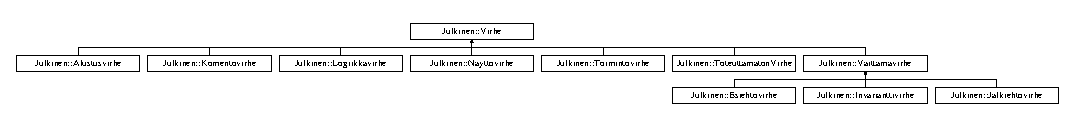
\includegraphics[height=1.160221cm]{class_julkinen_1_1_virhe}
\end{center}
\end{figure}
\subsection*{Public Member Functions}
\begin{DoxyCompactItemize}
\item 
\hyperlink{class_julkinen_1_1_virhe_a5a745aa6f700e7ea3a9b7f09e9ca5455}{Virhe} (std\+::string const \&virheviesti)
\begin{DoxyCompactList}\small\item\em Kopioidulla viestillä. \end{DoxyCompactList}\item 
\hyperlink{class_julkinen_1_1_virhe_a019192eb91000290fd9a36999532fb4b}{Virhe} (char const $\ast$virheviesti)
\begin{DoxyCompactList}\small\item\em Muualla tallessa olevalla viestillä. \end{DoxyCompactList}\item 
\hyperlink{class_julkinen_1_1_virhe_aba36e3156c54aa1281dc5be29b76af0a}{Virhe} (\hyperlink{class_julkinen_1_1_virhe}{Virhe} const \&toinen)
\begin{DoxyCompactList}\small\item\em Kopiorakentaja. \end{DoxyCompactList}\item 
virtual \hyperlink{class_julkinen_1_1_virhe_ab71f7f303930ccd1b48bda352412d625}{$\sim$\+Virhe} ()
\begin{DoxyCompactList}\small\item\em Purkaja. \end{DoxyCompactList}\item 
\hyperlink{class_julkinen_1_1_virhe}{Virhe} \& \hyperlink{class_julkinen_1_1_virhe_ad5ee9d8d642c20d464c6188088722492}{operator=} (\hyperlink{class_julkinen_1_1_virhe}{Virhe} const \&toinen)
\begin{DoxyCompactList}\small\item\em Sijoitusoperaattori. \end{DoxyCompactList}\item 
char const $\ast$ \hyperlink{class_julkinen_1_1_virhe_a14738e633b74fce18efbaf1086403013}{viesti} () const 
\begin{DoxyCompactList}\small\item\em Virheeseen liittyva ilmoitus. \end{DoxyCompactList}\item 
virtual std\+::basic\+\_\+ostream$<$ char $>$ \& \hyperlink{class_julkinen_1_1_virhe_a36a2644943038f9760b5d76a1960b00d}{tulosta} (std\+::basic\+\_\+ostream$<$ char $>$ \&tuloste) const 
\begin{DoxyCompactList}\small\item\em Tulosta virheen viesti virtaan. \end{DoxyCompactList}\end{DoxyCompactItemize}
\subsection*{Related Functions}
(Note that these are not member functions.) \begin{DoxyCompactItemize}
\item 
basic\+\_\+ostream$<$ char $>$ \& \hyperlink{class_julkinen_1_1_virhe_acc4933b244f9606f5349e6eb8ce37433}{operator$<$$<$} (basic\+\_\+ostream$<$ char $>$ \&tuloste, \hyperlink{class_julkinen_1_1_virhe}{Virhe} const \&virhe)
\begin{DoxyCompactList}\small\item\em Tulosta virhe. \end{DoxyCompactList}\item 
std\+::basic\+\_\+ostream$<$ char $>$ \& \hyperlink{class_julkinen_1_1_virhe_a41b6619bca23ba8db922973fdba25fc1}{operator$<$$<$} (std\+::basic\+\_\+ostream$<$ char $>$ \&tuloste, \hyperlink{class_julkinen_1_1_virhe}{Virhe} const \&virhe)
\begin{DoxyCompactList}\small\item\em Tulosta virhe. \end{DoxyCompactList}\end{DoxyCompactItemize}


\subsection{Detailed Description}
Labyrintin poikkeusten kantaluokka. 

Virheilmoitus voidaan antaa joko std\+::string-\/oliona kopioitavaksi, jolloin olion rakentaminesta voi tulla poikkeus, tai osoittimena C-\/merkkijonovakioon, jolloin rakentaminen on no-\/throw.

Mikäli virheilmoitukseen tarvitsee liittää muutakin kuin viesti, periytä luokasta uusi tyyppi, jolle tarvittavat tiedot voi antaa ja uudelleenmäärittele \hyperlink{class_julkinen_1_1_virhe_a36a2644943038f9760b5d76a1960b00d}{tulosta()}-\/metodi käyttämään näitä tietoja. 

\subsection{Constructor \& Destructor Documentation}
\hypertarget{class_julkinen_1_1_virhe_a5a745aa6f700e7ea3a9b7f09e9ca5455}{}\index{Julkinen\+::\+Virhe@{Julkinen\+::\+Virhe}!Virhe@{Virhe}}
\index{Virhe@{Virhe}!Julkinen\+::\+Virhe@{Julkinen\+::\+Virhe}}
\subsubsection[{Virhe(std\+::string const \&virheviesti)}]{\setlength{\rightskip}{0pt plus 5cm}Virhe\+::\+Virhe (
\begin{DoxyParamCaption}
\item[{std\+::string const \&}]{virheviesti}
\end{DoxyParamCaption}
)\hspace{0.3cm}{\ttfamily [explicit]}}\label{class_julkinen_1_1_virhe_a5a745aa6f700e7ea3a9b7f09e9ca5455}


Kopioidulla viestillä. 

\begin{DoxyPostcond}{Postcondition}
Perustakuu poikkeuksen sattuessa. 
\end{DoxyPostcond}

\begin{DoxyParams}{Parameters}
{\em virheviesti} & Merkkijono, joka kopioidaan poikkeuksen viestiksi. \\
\hline
\end{DoxyParams}

\begin{DoxyExceptions}{Exceptions}
{\em std\+::bad\+\_\+alloc} & Ei saatu varattua muistia viestiä varten. \\
\hline
\end{DoxyExceptions}
\hypertarget{class_julkinen_1_1_virhe_a019192eb91000290fd9a36999532fb4b}{}\index{Julkinen\+::\+Virhe@{Julkinen\+::\+Virhe}!Virhe@{Virhe}}
\index{Virhe@{Virhe}!Julkinen\+::\+Virhe@{Julkinen\+::\+Virhe}}
\subsubsection[{Virhe(char const $\ast$virheviesti)}]{\setlength{\rightskip}{0pt plus 5cm}Virhe\+::\+Virhe (
\begin{DoxyParamCaption}
\item[{char const $\ast$}]{virheviesti}
\end{DoxyParamCaption}
)\hspace{0.3cm}{\ttfamily [explicit]}}\label{class_julkinen_1_1_virhe_a019192eb91000290fd9a36999532fb4b}


Muualla tallessa olevalla viestillä. 

H\+U\+O\+M! Tämä luokka {\itshape ei} ota vastuuta osoittimen päässä olevan olion tuhoamisesta, eikä tee osoittimen osoittamasta tiedosta kopiota. Tarkoituksena on antaa osoitin esim. käännösyksikön tai luokan sisäiseen virheviestivakioon, jotta tämä rakentaja voi tarjota no-\/throw -\/takuun.

\begin{DoxyPostcond}{Postcondition}
No-\/throw -\/takuu. 
\end{DoxyPostcond}

\begin{DoxyParams}[1]{Parameters}
\mbox{\tt in}  & {\em virheviesti} & Osoitin oikeaan C-\/merkkijonovakioon tai vakioisen {\ttfamily std\+::string}-\/olion {\ttfamily c\+\_\+str()} metodin palauttamaan arvoon. \\
\hline
\end{DoxyParams}
\hypertarget{class_julkinen_1_1_virhe_aba36e3156c54aa1281dc5be29b76af0a}{}\index{Julkinen\+::\+Virhe@{Julkinen\+::\+Virhe}!Virhe@{Virhe}}
\index{Virhe@{Virhe}!Julkinen\+::\+Virhe@{Julkinen\+::\+Virhe}}
\subsubsection[{Virhe(\+Virhe const \&toinen)}]{\setlength{\rightskip}{0pt plus 5cm}Virhe\+::\+Virhe (
\begin{DoxyParamCaption}
\item[{{\bf Virhe} const \&}]{toinen}
\end{DoxyParamCaption}
)}\label{class_julkinen_1_1_virhe_aba36e3156c54aa1281dc5be29b76af0a}


Kopiorakentaja. 

\begin{DoxyPostcond}{Postcondition}
No-\/throw -\/takuu.
\end{DoxyPostcond}

\begin{DoxyParams}[1]{Parameters}
\mbox{\tt in}  & {\em toinen} & Kopioitava {\ttfamily \hyperlink{class_julkinen_1_1_virhe}{Virhe}}. \\
\hline
\end{DoxyParams}
\hypertarget{class_julkinen_1_1_virhe_ab71f7f303930ccd1b48bda352412d625}{}\index{Julkinen\+::\+Virhe@{Julkinen\+::\+Virhe}!````~Virhe@{$\sim$\+Virhe}}
\index{````~Virhe@{$\sim$\+Virhe}!Julkinen\+::\+Virhe@{Julkinen\+::\+Virhe}}
\subsubsection[{$\sim$\+Virhe()}]{\setlength{\rightskip}{0pt plus 5cm}Virhe\+::$\sim$\+Virhe (
\begin{DoxyParamCaption}
{}
\end{DoxyParamCaption}
)\hspace{0.3cm}{\ttfamily [virtual]}}\label{class_julkinen_1_1_virhe_ab71f7f303930ccd1b48bda352412d625}


Purkaja. 

\begin{DoxyPostcond}{Postcondition}
No-\/throw -\/takuu. 
\end{DoxyPostcond}


\subsection{Member Function Documentation}
\hypertarget{class_julkinen_1_1_virhe_ad5ee9d8d642c20d464c6188088722492}{}\index{Julkinen\+::\+Virhe@{Julkinen\+::\+Virhe}!operator=@{operator=}}
\index{operator=@{operator=}!Julkinen\+::\+Virhe@{Julkinen\+::\+Virhe}}
\subsubsection[{operator=(\+Virhe const \&toinen)}]{\setlength{\rightskip}{0pt plus 5cm}{\bf Virhe} \& Virhe\+::operator= (
\begin{DoxyParamCaption}
\item[{{\bf Virhe} const \&}]{toinen}
\end{DoxyParamCaption}
)}\label{class_julkinen_1_1_virhe_ad5ee9d8d642c20d464c6188088722492}


Sijoitusoperaattori. 

\begin{DoxyPostcond}{Postcondition}
No-\/throw -\/takuu.
\end{DoxyPostcond}

\begin{DoxyParams}[1]{Parameters}
\mbox{\tt in}  & {\em toinen} & Sijoitettava {\ttfamily \hyperlink{class_julkinen_1_1_virhe}{Virhe}}. \\
\hline
\end{DoxyParams}
\hypertarget{class_julkinen_1_1_virhe_a36a2644943038f9760b5d76a1960b00d}{}\index{Julkinen\+::\+Virhe@{Julkinen\+::\+Virhe}!tulosta@{tulosta}}
\index{tulosta@{tulosta}!Julkinen\+::\+Virhe@{Julkinen\+::\+Virhe}}
\subsubsection[{tulosta(std\+::basic\+\_\+ostream$<$ char $>$ \&tuloste) const }]{\setlength{\rightskip}{0pt plus 5cm}basic\+\_\+ostream$<$ char $>$ \& Virhe\+::tulosta (
\begin{DoxyParamCaption}
\item[{std\+::basic\+\_\+ostream$<$ char $>$ \&}]{tuloste}
\end{DoxyParamCaption}
) const\hspace{0.3cm}{\ttfamily [virtual]}}\label{class_julkinen_1_1_virhe_a36a2644943038f9760b5d76a1960b00d}


Tulosta virheen viesti virtaan. 

Tulostaa virheen viestin virtaan, eikä tee muuta.

\begin{DoxyPostcond}{Postcondition}
Vahva poikkeustakuu. 
\end{DoxyPostcond}

\begin{DoxyParams}[1]{Parameters}
\mbox{\tt in}  & {\em tuloste} & Virta, jonne viesti tulostetaan. \\
\hline
\end{DoxyParams}
\begin{DoxyReturn}{Returns}
{\ttfamily tuloste} 
\end{DoxyReturn}


Reimplemented in \hyperlink{class_julkinen_1_1_toimintovirhe_a6a3078478f0bbf08821d0d5357df2c6a}{Julkinen\+::\+Toimintovirhe}, \hyperlink{class_julkinen_1_1_komentovirhe_a51d6d273b79074b6c8ea8d0b1ef2fe65}{Julkinen\+::\+Komentovirhe}, \hyperlink{class_julkinen_1_1_alustusvirhe_a22b50252a516b339d126261978fb62c1}{Julkinen\+::\+Alustusvirhe}, \hyperlink{class_julkinen_1_1_vaittamavirhe_a5ca289035ecde35b1b1576d1c9219acd}{Julkinen\+::\+Vaittamavirhe}, \hyperlink{class_julkinen_1_1_nayttovirhe_ae8e4d0a5f98c3f61afc72dfed2af967f}{Julkinen\+::\+Nayttovirhe}, \hyperlink{class_julkinen_1_1_logiikkavirhe_a298ce4b9c3d1887d5be431bea89645da}{Julkinen\+::\+Logiikkavirhe}, \hyperlink{class_julkinen_1_1_esiehtovirhe_a333610e4679e467075bd02c37b9e49bf}{Julkinen\+::\+Esiehtovirhe}, \hyperlink{class_julkinen_1_1_invarianttivirhe_ac0f90f4d0915c90c14d752a64da5196a}{Julkinen\+::\+Invarianttivirhe}, and \hyperlink{class_julkinen_1_1_jalkiehtovirhe_a5cbdae2671dfaa4700a9118048c7570e}{Julkinen\+::\+Jalkiehtovirhe}.

\hypertarget{class_julkinen_1_1_virhe_a14738e633b74fce18efbaf1086403013}{}\index{Julkinen\+::\+Virhe@{Julkinen\+::\+Virhe}!viesti@{viesti}}
\index{viesti@{viesti}!Julkinen\+::\+Virhe@{Julkinen\+::\+Virhe}}
\subsubsection[{viesti() const }]{\setlength{\rightskip}{0pt plus 5cm}char const $\ast$ Virhe\+::viesti (
\begin{DoxyParamCaption}
{}
\end{DoxyParamCaption}
) const}\label{class_julkinen_1_1_virhe_a14738e633b74fce18efbaf1086403013}


Virheeseen liittyva ilmoitus. 

\begin{DoxyPostcond}{Postcondition}
No-\/throw -\/takuu. 
\end{DoxyPostcond}


\subsection{Friends And Related Function Documentation}
\hypertarget{class_julkinen_1_1_virhe_acc4933b244f9606f5349e6eb8ce37433}{}\index{Julkinen\+::\+Virhe@{Julkinen\+::\+Virhe}!operator$<$$<$@{operator$<$$<$}}
\index{operator$<$$<$@{operator$<$$<$}!Julkinen\+::\+Virhe@{Julkinen\+::\+Virhe}}
\subsubsection[{operator$<$$<$(basic\+\_\+ostream$<$ char $>$ \&tuloste, Virhe const \&virhe)}]{\setlength{\rightskip}{0pt plus 5cm}basic\+\_\+ostream$<$ char $>$ \& operator$<$$<$ (
\begin{DoxyParamCaption}
\item[{basic\+\_\+ostream$<$ char $>$ \&}]{tuloste, }
\item[{{\bf Virhe} const \&}]{virhe}
\end{DoxyParamCaption}
)\hspace{0.3cm}{\ttfamily [related]}}\label{class_julkinen_1_1_virhe_acc4933b244f9606f5349e6eb8ce37433}


Tulosta virhe. 

\hyperlink{class_julkinen_1_1_virhe}{Virhe} tulostetaan \hyperlink{class_julkinen_1_1_virhe_a36a2644943038f9760b5d76a1960b00d}{Virhe\+::tulosta()}-\/metodilla.


\begin{DoxyParams}[1]{Parameters}
\mbox{\tt in,out}  & {\em tuloste} & Virta jonne tulostetaan. \\
\hline
\mbox{\tt in}  & {\em virhe} & Tulostettava \hyperlink{class_julkinen_1_1_virhe}{Virhe}. \\
\hline
\end{DoxyParams}
\begin{DoxyReturn}{Returns}
{\ttfamily tuloste} 
\end{DoxyReturn}
\hypertarget{class_julkinen_1_1_virhe_a41b6619bca23ba8db922973fdba25fc1}{}\index{Julkinen\+::\+Virhe@{Julkinen\+::\+Virhe}!operator$<$$<$@{operator$<$$<$}}
\index{operator$<$$<$@{operator$<$$<$}!Julkinen\+::\+Virhe@{Julkinen\+::\+Virhe}}
\subsubsection[{operator$<$$<$(std\+::basic\+\_\+ostream$<$ char $>$ \&tuloste, Virhe const \&virhe)}]{\setlength{\rightskip}{0pt plus 5cm}std\+::basic\+\_\+ostream$<$ char $>$ \& operator$<$$<$ (
\begin{DoxyParamCaption}
\item[{std\+::basic\+\_\+ostream$<$ char $>$ \&}]{tuloste, }
\item[{{\bf Virhe} const \&}]{virhe}
\end{DoxyParamCaption}
)\hspace{0.3cm}{\ttfamily [related]}}\label{class_julkinen_1_1_virhe_a41b6619bca23ba8db922973fdba25fc1}


Tulosta virhe. 

\hyperlink{class_julkinen_1_1_virhe}{Virhe} tulostetaan \hyperlink{class_julkinen_1_1_virhe_a36a2644943038f9760b5d76a1960b00d}{Virhe\+::tulosta()}-\/metodilla.


\begin{DoxyParams}[1]{Parameters}
\mbox{\tt in,out}  & {\em tuloste} & Virta jonne tulostetaan. \\
\hline
\mbox{\tt in}  & {\em virhe} & Tulostettava virhe. \\
\hline
\end{DoxyParams}
\begin{DoxyReturn}{Returns}
{\ttfamily tuloste} 
\end{DoxyReturn}


The documentation for this class was generated from the following files\+:\begin{DoxyCompactItemize}
\item 
\hyperlink{virhe_8hh}{virhe.\+hh}\item 
valmiiden\+\_\+toteutus/\hyperlink{virhe_8cc}{virhe.\+cc}\end{DoxyCompactItemize}

\chapter{File Documentation}
\hypertarget{alustusvirhe_8hh}{}\section{alustusvirhe.\+hh File Reference}
\label{alustusvirhe_8hh}\index{alustusvirhe.\+hh@{alustusvirhe.\+hh}}


Alustusvirhe-\/luokan esittely. (.  


{\ttfamily \#include \char`\"{}virhe.\+hh\char`\"{}}\\*
\subsection*{Classes}
\begin{DoxyCompactItemize}
\item 
class \hyperlink{class_julkinen_1_1_alustusvirhe}{Julkinen\+::\+Alustusvirhe}
\begin{DoxyCompactList}\small\item\em Alustuksessa tapahtuvaa virhettä kuvaava poikkeus. \end{DoxyCompactList}\end{DoxyCompactItemize}
\subsection*{Namespaces}
\begin{DoxyCompactItemize}
\item 
 \hyperlink{namespace_julkinen}{Julkinen}
\begin{DoxyCompactList}\small\item\em Luo instanssi pelirajapinnasta. \end{DoxyCompactList}\end{DoxyCompactItemize}


\subsection{Detailed Description}
Alustusvirhe-\/luokan esittely. (. 

\begin{DoxyVersion}{Version}

\end{DoxyVersion}
\begin{DoxyParagraph}{Id}
\hyperlink{alustusvirhe_8hh}{alustusvirhe.\+hh} 2660 2013-\/02-\/15 10\+:27\+:37\+Z bitti 
\end{DoxyParagraph}


\begin{DoxyParagraph}{Revision}
2660 
\end{DoxyParagraph}
) \begin{DoxyAuthor}{Author}
©2010 Eero Salonen \href{mailto:eero.j.salonen@tut.fi}{\tt eero.\+j.\+salonen@tut.\+fi} 
\end{DoxyAuthor}

\hypertarget{_data_8hpp}{}\section{Data.\+hpp File Reference}
\label{_data_8hpp}\index{Data.\+hpp@{Data.\+hpp}}


Data-\/luokan esittely.  


{\ttfamily \#include \char`\"{}luettelotyypit.\+hh\char`\"{}}\\*
{\ttfamily \#include \char`\"{}koordinaatti.\+hh\char`\"{}}\\*
{\ttfamily \#include \char`\"{}alustusvirhe.\+hh\char`\"{}}\\*
{\ttfamily \#include \char`\"{}Pelaaja.\+hpp\char`\"{}}\\*
{\ttfamily \#include \char`\"{}Esine.\+hpp\char`\"{}}\\*
{\ttfamily \#include \char`\"{}Pala.\+hpp\char`\"{}}\\*
{\ttfamily \#include $<$vector$>$}\\*
{\ttfamily \#include $<$map$>$}\\*
\subsection*{Classes}
\begin{DoxyCompactItemize}
\item 
class \hyperlink{class_data}{Data}
\end{DoxyCompactItemize}


\subsection{Detailed Description}
Data-\/luokan esittely. 

\begin{DoxyVersion}{Version}

\end{DoxyVersion}
\begin{DoxyParagraph}{Id}
\hyperlink{_data_8hpp}{Data.\+hpp} 2660 2015-\/12-\/08 12\+:47\+:00\+Z bitti 
\end{DoxyParagraph}


\begin{DoxyAuthor}{Author}
©2015 Santeri Hetekivi \href{mailto:santeri.hetekivi@eng.tamk.fi}{\tt santeri.\+hetekivi@eng.\+tamk.\+fi} 
\end{DoxyAuthor}

\hypertarget{debug_8hh}{}\section{debug.\+hh File Reference}
\label{debug_8hh}\index{debug.\+hh@{debug.\+hh}}


Debuggauksen apumakro.  


{\ttfamily \#include $<$iostream$>$}\\*
\subsection*{Macros}
\begin{DoxyCompactItemize}
\item 
\#define \hyperlink{debug_8hh_a3dad2c39ac6dc7758661440350fabb11}{D\+E\+B\+U\+G\+\_\+\+O\+U\+T\+P\+U\+T}(stuff)~if (\hyperlink{labyrintti_8cc_ab9eefb6ae2797c531d0b6e8c8264cdfa}{debug\+\_\+output}) \{  stuff ; \}
\begin{DoxyCompactList}\small\item\em Makro, jolla voi tulostaa debug-\/tulosteita. \end{DoxyCompactList}\end{DoxyCompactItemize}
\subsection*{Variables}
\begin{DoxyCompactItemize}
\item 
bool \hyperlink{debug_8hh_ab9eefb6ae2797c531d0b6e8c8264cdfa}{debug\+\_\+output}
\begin{DoxyCompactList}\small\item\em Globaali debug-\/lippu. \end{DoxyCompactList}\end{DoxyCompactItemize}


\subsection{Detailed Description}
Debuggauksen apumakro. 

\begin{DoxyAuthor}{Author}
©2011 Matti Rintala \href{mailto:bitti@cs.tut.fi}{\tt bitti@cs.\+tut.\+fi}, T\+T\+Y Ohjelmistotekniikka 
\end{DoxyAuthor}


\subsection{Macro Definition Documentation}
\hypertarget{debug_8hh_a3dad2c39ac6dc7758661440350fabb11}{}\index{debug.\+hh@{debug.\+hh}!D\+E\+B\+U\+G\+\_\+\+O\+U\+T\+P\+U\+T@{D\+E\+B\+U\+G\+\_\+\+O\+U\+T\+P\+U\+T}}
\index{D\+E\+B\+U\+G\+\_\+\+O\+U\+T\+P\+U\+T@{D\+E\+B\+U\+G\+\_\+\+O\+U\+T\+P\+U\+T}!debug.\+hh@{debug.\+hh}}
\subsubsection[{D\+E\+B\+U\+G\+\_\+\+O\+U\+T\+P\+U\+T}]{\setlength{\rightskip}{0pt plus 5cm}\#define D\+E\+B\+U\+G\+\_\+\+O\+U\+T\+P\+U\+T(
\begin{DoxyParamCaption}
\item[{}]{stuff}
\end{DoxyParamCaption}
)~if ({\bf debug\+\_\+output}) \{  stuff ; \}}\label{debug_8hh_a3dad2c39ac6dc7758661440350fabb11}


Makro, jolla voi tulostaa debug-\/tulosteita. 

{\bfseries Tämän makron toteutus on vielä kesken!}

Käytetään seuraavasti\+: 
\begin{DoxyCode}
1 DEBUG\_OUTPUT("Kääk" << std::endl);
\end{DoxyCode}


\begin{DoxyPostcond}{Postcondition}
Jos ohjelma on käännetty debug-\/tilassa, tulostus tulostuu ruudulle. Muussa tapauksessa mitään ei tapahdu. 
\end{DoxyPostcond}


\subsection{Variable Documentation}
\hypertarget{debug_8hh_ab9eefb6ae2797c531d0b6e8c8264cdfa}{}\index{debug.\+hh@{debug.\+hh}!debug\+\_\+output@{debug\+\_\+output}}
\index{debug\+\_\+output@{debug\+\_\+output}!debug.\+hh@{debug.\+hh}}
\subsubsection[{debug\+\_\+output}]{\setlength{\rightskip}{0pt plus 5cm}bool debug\+\_\+output}\label{debug_8hh_ab9eefb6ae2797c531d0b6e8c8264cdfa}


Globaali debug-\/lippu. 

Pääohjelma asettaa tämän lipun, jos ohjelma on käynnistetty debug-\/optiolla 
\hypertarget{_esine_8hpp}{}\section{Esine.\+hpp File Reference}
\label{_esine_8hpp}\index{Esine.\+hpp@{Esine.\+hpp}}


Esine-\/luokan esittely.  


{\ttfamily \#include $<$string$>$}\\*
\subsection*{Classes}
\begin{DoxyCompactItemize}
\item 
class \hyperlink{class_esine}{Esine}
\begin{DoxyCompactList}\small\item\em Labyrintti-\/pelin esineen tietoluokka. \end{DoxyCompactList}\end{DoxyCompactItemize}


\subsection{Detailed Description}
Esine-\/luokan esittely. 

\begin{DoxyVersion}{Version}

\end{DoxyVersion}
\begin{DoxyParagraph}{Id}
\hyperlink{_esine_8hpp}{Esine.\+hpp} 2660 2015-\/12-\/08 12\+:47\+:00\+Z bitti 
\end{DoxyParagraph}


\begin{DoxyAuthor}{Author}
©2015 Santeri Hetekivi \href{mailto:santeri.hetekivi@eng.tamk.fi}{\tt santeri.\+hetekivi@eng.\+tamk.\+fi} 
\end{DoxyAuthor}

\hypertarget{komentovirhe_8hh}{}\section{komentovirhe.\+hh File Reference}
\label{komentovirhe_8hh}\index{komentovirhe.\+hh@{komentovirhe.\+hh}}


Komentovirhe-\/luokan esittely.  


{\ttfamily \#include \char`\"{}virhe.\+hh\char`\"{}}\\*
\subsection*{Classes}
\begin{DoxyCompactItemize}
\item 
class \hyperlink{class_julkinen_1_1_komentovirhe}{Julkinen\+::\+Komentovirhe}
\begin{DoxyCompactList}\small\item\em Käyttäjän antamaa pelikomentoa ei saatu suoritettua. \end{DoxyCompactList}\end{DoxyCompactItemize}
\subsection*{Namespaces}
\begin{DoxyCompactItemize}
\item 
 \hyperlink{namespace_julkinen}{Julkinen}
\begin{DoxyCompactList}\small\item\em Luo instanssi pelirajapinnasta. \end{DoxyCompactList}\end{DoxyCompactItemize}


\subsection{Detailed Description}
Komentovirhe-\/luokan esittely. 

\begin{DoxyVersion}{Version}

\end{DoxyVersion}
\begin{DoxyParagraph}{Id}
\hyperlink{komentovirhe_8hh}{komentovirhe.\+hh} 2660 2013-\/02-\/15 10\+:27\+:37\+Z bitti 
\end{DoxyParagraph}


\begin{DoxyAuthor}{Author}
©2010 Eero Salonen \href{mailto:eero.j.salonen@tut.fi}{\tt eero.\+j.\+salonen@tut.\+fi} 
\end{DoxyAuthor}

\hypertarget{koordinaatti_8hh}{}\section{koordinaatti.\+hh File Reference}
\label{koordinaatti_8hh}\index{koordinaatti.\+hh@{koordinaatti.\+hh}}


Koordinaatti-\/luokan esittely. (.  


\subsection*{Classes}
\begin{DoxyCompactItemize}
\item 
class \hyperlink{class_julkinen_1_1_koordinaatti}{Julkinen\+::\+Koordinaatti}
\begin{DoxyCompactList}\small\item\em Luokka pelin sijainti tietojen esittämiseen. \end{DoxyCompactList}\end{DoxyCompactItemize}
\subsection*{Namespaces}
\begin{DoxyCompactItemize}
\item 
 \hyperlink{namespace_julkinen}{Julkinen}
\begin{DoxyCompactList}\small\item\em Luo instanssi pelirajapinnasta. \end{DoxyCompactList}\end{DoxyCompactItemize}


\subsection{Detailed Description}
Koordinaatti-\/luokan esittely. (. 

\begin{DoxyVersion}{Version}

\end{DoxyVersion}
\begin{DoxyParagraph}{Id}
\hyperlink{koordinaatti_8hh}{koordinaatti.\+hh} 2735 2013-\/04-\/18 11\+:35\+:51\+Z bitti 
\end{DoxyParagraph}


\begin{DoxyParagraph}{Revision}
2735 
\end{DoxyParagraph}
) \begin{DoxyAuthor}{Author}
©2010 Eero Salonen \href{mailto:eero.j.salonen@tut.fi}{\tt eero.\+j.\+salonen@tut.\+fi} 
\end{DoxyAuthor}

\hypertarget{logiikkavirhe_8hh}{}\section{logiikkavirhe.\+hh File Reference}
\label{logiikkavirhe_8hh}\index{logiikkavirhe.\+hh@{logiikkavirhe.\+hh}}


Logiikkavirhe-\/luokan esittely.  


{\ttfamily \#include \char`\"{}virhe.\+hh\char`\"{}}\\*
\subsection*{Classes}
\begin{DoxyCompactItemize}
\item 
class \hyperlink{class_julkinen_1_1_logiikkavirhe}{Julkinen\+::\+Logiikkavirhe}
\begin{DoxyCompactList}\small\item\em \hyperlink{class_julkinen_1_1_virhe}{Virhe} toimintalogiikka virhetilanteita varten. \end{DoxyCompactList}\end{DoxyCompactItemize}
\subsection*{Namespaces}
\begin{DoxyCompactItemize}
\item 
 \hyperlink{namespace_julkinen}{Julkinen}
\begin{DoxyCompactList}\small\item\em Luo instanssi pelirajapinnasta. \end{DoxyCompactList}\end{DoxyCompactItemize}


\subsection{Detailed Description}
Logiikkavirhe-\/luokan esittely. 

\begin{DoxyVersion}{Version}

\end{DoxyVersion}
\begin{DoxyParagraph}{Id}
\hyperlink{koordinaatti_8cc}{koordinaatti.\+cc} 1797 2011-\/02-\/03 01\+:56\+:31\+Z salone58 
\end{DoxyParagraph}


\begin{DoxyAuthor}{Author}
©2010 Eero Salonen \href{mailto:eero.j.salonen@tut.fi}{\tt eero.\+j.\+salonen@tut.\+fi} 
\end{DoxyAuthor}

\hypertarget{luettelotyypit_8hh}{}\section{luettelotyypit.\+hh File Reference}
\label{luettelotyypit_8hh}\index{luettelotyypit.\+hh@{luettelotyypit.\+hh}}


Pelirajapinta-\/luokan esittely. (.  


\subsection*{Namespaces}
\begin{DoxyCompactItemize}
\item 
 \hyperlink{namespace_julkinen}{Julkinen}
\begin{DoxyCompactList}\small\item\em Luo instanssi pelirajapinnasta. \end{DoxyCompactList}\end{DoxyCompactItemize}
\subsection*{Enumerations}
\begin{DoxyCompactItemize}
\item 
enum \hyperlink{namespace_julkinen_a81b50e3c6f21c0c1c46e186592107c3c}{Julkinen\+::\+Suunta} \{ \\*
\hyperlink{namespace_julkinen_a81b50e3c6f21c0c1c46e186592107c3cacae80e18deb2f6685d0bf0f174042ec2}{Julkinen\+::\+A\+L\+A\+S}, 
\hyperlink{namespace_julkinen_a81b50e3c6f21c0c1c46e186592107c3ca989d727d65ca4aea941b51638e642596}{Julkinen\+::\+A\+U\+T\+O\+M\+A\+A\+T\+T\+I}, 
\hyperlink{namespace_julkinen_a81b50e3c6f21c0c1c46e186592107c3cafd8f13dddbcf5e33a9c33a4cdae76f59}{Julkinen\+::\+O\+I\+K\+E\+A\+L\+L\+E}, 
\hyperlink{namespace_julkinen_a81b50e3c6f21c0c1c46e186592107c3ca4b3b91fdb43fdb60e03fb47b23c78e03}{Julkinen\+::\+V\+A\+S\+E\+M\+M\+A\+L\+L\+E}, 
\\*
\hyperlink{namespace_julkinen_a81b50e3c6f21c0c1c46e186592107c3caa9a06721d0cc8ff51b1071d3962841ee}{Julkinen\+::\+Y\+L\+O\+S}, 
\hyperlink{namespace_julkinen_a81b50e3c6f21c0c1c46e186592107c3cafa60a1b03bc49af14fb90b7026f94957}{Julkinen\+::\+P\+A\+I\+K\+A\+L\+L\+A\+A\+N}
 \}\begin{DoxyCompactList}\small\item\em Pelaajan liikumissuunnat. \end{DoxyCompactList}
\item 
enum \hyperlink{namespace_julkinen_afc26052e09d0b2214f749492cc5fff19}{Julkinen\+::\+Erikoispala\+Tyyppi} \{ \hyperlink{namespace_julkinen_afc26052e09d0b2214f749492cc5fff19a67d9c76baa2a4eec4ca132c15bd567b5}{Julkinen\+::\+N\+O\+R\+M\+A\+A\+L\+I}, 
\hyperlink{namespace_julkinen_afc26052e09d0b2214f749492cc5fff19aec227daa1859a2163571035e354c97b4}{Julkinen\+::\+T\+E\+L\+E\+P\+O\+R\+T\+T\+I}, 
\hyperlink{namespace_julkinen_afc26052e09d0b2214f749492cc5fff19aa50081048583c91c88ed285cad5d3080}{Julkinen\+::\+S\+I\+U\+N\+A\+T\+T\+U}, 
\hyperlink{namespace_julkinen_afc26052e09d0b2214f749492cc5fff19a8a097f13eb73d7bf4d8cd14dea73ce24}{Julkinen\+::\+K\+I\+R\+O\+T\+T\+U}
 \}\begin{DoxyCompactList}\small\item\em Esineiden tyyppitieto. \end{DoxyCompactList}
\item 
enum \hyperlink{namespace_julkinen_ad9a0a9e01af78249f584a93b03db4329}{Julkinen\+::\+Pelaaja\+Tyyppi} \{ \hyperlink{namespace_julkinen_ad9a0a9e01af78249f584a93b03db4329ac071c9196447e9db07e03619140a21a9}{Julkinen\+::\+I\+H\+M\+I\+N\+E\+N}, 
\hyperlink{namespace_julkinen_ad9a0a9e01af78249f584a93b03db4329a72363d3abdcf0ff5a5318785a7d18363}{Julkinen\+::\+T\+I\+E\+T\+O\+K\+O\+N\+E}
 \}\begin{DoxyCompactList}\small\item\em Tieto millainen pelaaja on kyseessä \end{DoxyCompactList}
\item 
enum \hyperlink{namespace_julkinen_a272c70e0503191a485c8a9cd4281e6f5}{Julkinen\+::\+Pala\+Tyyppi} \{ \hyperlink{namespace_julkinen_a272c70e0503191a485c8a9cd4281e6f5abda0f6d812200f15d8486fa03a5e24d5}{Julkinen\+::\+I\+P\+A\+L\+A}, 
\hyperlink{namespace_julkinen_a272c70e0503191a485c8a9cd4281e6f5aca28caf9f024aa0f392fe0242f5e31f4}{Julkinen\+::\+L\+P\+A\+L\+A}, 
\hyperlink{namespace_julkinen_a272c70e0503191a485c8a9cd4281e6f5ad52333f7493bd772341097ab62f7eba3}{Julkinen\+::\+T\+P\+A\+L\+A}
 \}\begin{DoxyCompactList}\small\item\em Tieto siitä minkämuotoinen pala on kyseessä \end{DoxyCompactList}
\item 
enum \hyperlink{namespace_julkinen_acce0eefc4c90f907dd5fb319b0d05872}{Julkinen\+::\+Reuna} \{ \\*
\hyperlink{namespace_julkinen_acce0eefc4c90f907dd5fb319b0d05872ae751031a265231a493641ba564930530}{Julkinen\+::\+A\+L\+A}, 
\hyperlink{namespace_julkinen_acce0eefc4c90f907dd5fb319b0d05872ae4725f066287e0db7262b3981a2756d6}{Julkinen\+::\+O\+I\+K\+E\+A}, 
\hyperlink{namespace_julkinen_acce0eefc4c90f907dd5fb319b0d05872a15b788f98845dd777cba865f4ad12cce}{Julkinen\+::\+V\+A\+S\+E\+N}, 
\hyperlink{namespace_julkinen_acce0eefc4c90f907dd5fb319b0d05872ad0f36cc10711b6b9d5141e86d02e8040}{Julkinen\+::\+Y\+L\+A}, 
\\*
\hyperlink{namespace_julkinen_acce0eefc4c90f907dd5fb319b0d05872a0ce6aecd0ad5ab9e7311506949a7d2c8}{Julkinen\+::\+E\+I\+O\+L\+E}
 \}\begin{DoxyCompactList}\small\item\em Tieto mille reunalle irtopala työnnettiin. \end{DoxyCompactList}
\end{DoxyCompactItemize}


\subsection{Detailed Description}
Pelirajapinta-\/luokan esittely. (. 

\begin{DoxyVersion}{Version}

\end{DoxyVersion}
\begin{DoxyParagraph}{Id}
\hyperlink{pelirajapinta_8hh}{pelirajapinta.\+hh} 1844 2011-\/02-\/13 22\+:10\+:37\+Z salone58 
\end{DoxyParagraph}


\begin{DoxyParagraph}{Revision}
1844 
\end{DoxyParagraph}
) \begin{DoxyAuthor}{Author}
©2011 Eero Salonen \href{mailto:eero.j.salonen@tut.fi}{\tt eero.\+j.\+salonen@tut.\+fi} 
\end{DoxyAuthor}

\hypertarget{nayttorajapinta_8hh}{}\section{nayttorajapinta.\+hh File Reference}
\label{nayttorajapinta_8hh}\index{nayttorajapinta.\+hh@{nayttorajapinta.\+hh}}


Rajapinta pelin luomiseksi (.  


{\ttfamily \#include \char`\"{}luettelotyypit.\+hh\char`\"{}}\\*
{\ttfamily \#include \char`\"{}koordinaatti.\+hh\char`\"{}}\\*
{\ttfamily \#include $<$string$>$}\\*
\subsection*{Classes}
\begin{DoxyCompactItemize}
\item 
class \hyperlink{class_julkinen_1_1_nayttorajapinta}{Julkinen\+::\+Nayttorajapinta}
\begin{DoxyCompactList}\small\item\em Labyrintti-\/pelin tulostusrajapinta. \end{DoxyCompactList}\end{DoxyCompactItemize}
\subsection*{Namespaces}
\begin{DoxyCompactItemize}
\item 
 \hyperlink{namespace_julkinen}{Julkinen}
\begin{DoxyCompactList}\small\item\em Luo instanssi pelirajapinnasta. \end{DoxyCompactList}\end{DoxyCompactItemize}


\subsection{Detailed Description}
Rajapinta pelin luomiseksi (. 

\begin{DoxyVersion}{Version}

\end{DoxyVersion}
\begin{DoxyParagraph}{Id}
\hyperlink{nayttorajapinta_8hh}{nayttorajapinta.\+hh} 2677 2013-\/02-\/20 13\+:03\+:17\+Z voutilai 
\end{DoxyParagraph}


\begin{DoxyParagraph}{Revision}
2677 
\end{DoxyParagraph}
) \begin{DoxyAuthor}{Author}
©2010 Eero Salonen $<$\href{mailto:eero.j.salonen@tut.fi}{\tt eero.\+j.\+salonen@tut.\+fi} 
\end{DoxyAuthor}

\hypertarget{nayttovirhe_8hh}{}\section{nayttovirhe.\+hh File Reference}
\label{nayttovirhe_8hh}\index{nayttovirhe.\+hh@{nayttovirhe.\+hh}}


Nayttovirhe-\/luokan esittely.  


{\ttfamily \#include \char`\"{}virhe.\+hh\char`\"{}}\\*
\subsection*{Classes}
\begin{DoxyCompactItemize}
\item 
class \hyperlink{class_julkinen_1_1_nayttovirhe}{Julkinen\+::\+Nayttovirhe}
\begin{DoxyCompactList}\small\item\em Näyttörajapinnan tulostusoperaatio ei onnistunut. \end{DoxyCompactList}\end{DoxyCompactItemize}
\subsection*{Namespaces}
\begin{DoxyCompactItemize}
\item 
 \hyperlink{namespace_julkinen}{Julkinen}
\begin{DoxyCompactList}\small\item\em Luo instanssi pelirajapinnasta. \end{DoxyCompactList}\end{DoxyCompactItemize}


\subsection{Detailed Description}
Nayttovirhe-\/luokan esittely. 

\begin{DoxyVersion}{Version}

\end{DoxyVersion}
\begin{DoxyParagraph}{Id}
\hyperlink{nayttovirhe_8hh}{nayttovirhe.\+hh} 2660 2013-\/02-\/15 10\+:27\+:37\+Z bitti 
\end{DoxyParagraph}


\begin{DoxyAuthor}{Author}
©2010 Eero Salonen \href{mailto:eero.j.salonen@tut.fi}{\tt eero.\+j.\+salonen@tut.\+fi} 
\end{DoxyAuthor}

\hypertarget{_pala_8hpp}{}\section{Pala.\+hpp File Reference}
\label{_pala_8hpp}\index{Pala.\+hpp@{Pala.\+hpp}}


Pala-\/luokan esittely.  


{\ttfamily \#include \char`\"{}koordinaatti.\+hh\char`\"{}}\\*
{\ttfamily \#include \char`\"{}luettelotyypit.\+hh\char`\"{}}\\*
{\ttfamily \#include \char`\"{}Esine.\+hpp\char`\"{}}\\*
{\ttfamily \#include \char`\"{}Pelaaja.\+hpp\char`\"{}}\\*
\subsection*{Classes}
\begin{DoxyCompactItemize}
\item 
class \hyperlink{class_pala}{Pala}
\begin{DoxyCompactList}\small\item\em Labyrintti-\/pelin palan tietoluokka. \end{DoxyCompactList}\end{DoxyCompactItemize}


\subsection{Detailed Description}
Pala-\/luokan esittely. 

\begin{DoxyVersion}{Version}

\end{DoxyVersion}
\begin{DoxyParagraph}{Id}
\hyperlink{_pala_8hpp}{Pala.\+hpp} 2660 2015-\/12-\/08 12\+:47\+:00\+Z bitti 
\end{DoxyParagraph}


\begin{DoxyAuthor}{Author}
©2015 Santeri Hetekivi \href{mailto:santeri.hetekivi@eng.tamk.fi}{\tt santeri.\+hetekivi@eng.\+tamk.\+fi} 
\end{DoxyAuthor}

\hypertarget{_pelaaja_8hpp}{}\section{Pelaaja.\+hpp File Reference}
\label{_pelaaja_8hpp}\index{Pelaaja.\+hpp@{Pelaaja.\+hpp}}


Pelaaja-\/luokan esittely.  


{\ttfamily \#include \char`\"{}luettelotyypit.\+hh\char`\"{}}\\*
{\ttfamily \#include \char`\"{}Esine.\+hpp\char`\"{}}\\*
{\ttfamily \#include $<$queue$>$}\\*
{\ttfamily \#include $<$vector$>$}\\*
\subsection*{Classes}
\begin{DoxyCompactItemize}
\item 
class \hyperlink{class_pelaaja}{Pelaaja}
\begin{DoxyCompactList}\small\item\em Labyrintti-\/pelin pelaajan tietoluokka. \end{DoxyCompactList}\end{DoxyCompactItemize}


\subsection{Detailed Description}
Pelaaja-\/luokan esittely. 

\begin{DoxyVersion}{Version}

\end{DoxyVersion}
\begin{DoxyParagraph}{Id}
\hyperlink{_pelaaja_8hpp}{Pelaaja.\+hpp} 2660 2015-\/12-\/08 12\+:47\+:00\+Z bitti 
\end{DoxyParagraph}


\begin{DoxyAuthor}{Author}
©2015 Santeri Hetekivi \href{mailto:santeri.hetekivi@eng.tamk.fi}{\tt santeri.\+hetekivi@eng.\+tamk.\+fi} 
\end{DoxyAuthor}

\hypertarget{_pelaaja_toiminto_8hpp}{}\section{Pelaaja\+Toiminto.\+hpp File Reference}
\label{_pelaaja_toiminto_8hpp}\index{Pelaaja\+Toiminto.\+hpp@{Pelaaja\+Toiminto.\+hpp}}


Pelaaja\+Toiminto-\/luokan esittely.  


{\ttfamily \#include \char`\"{}Pelin\+Naytto.\+hpp\char`\"{}}\\*
{\ttfamily \#include \char`\"{}luettelotyypit.\+hh\char`\"{}}\\*
{\ttfamily \#include \char`\"{}koordinaatti.\+hh\char`\"{}}\\*
{\ttfamily \#include \char`\"{}vaittama.\+hh\char`\"{}}\\*
{\ttfamily \#include \char`\"{}toimintovirhe.\+hh\char`\"{}}\\*
{\ttfamily \#include $<$stdlib.\+h$>$}\\*
{\ttfamily \#include $<$time.\+h$>$}\\*
\subsection*{Classes}
\begin{DoxyCompactItemize}
\item 
class \hyperlink{class_pelaaja_toiminto}{Pelaaja\+Toiminto}
\begin{DoxyCompactList}\small\item\em Labyrintti-\/pelin pelaajan toimintojen suoritus luokka. \end{DoxyCompactList}\end{DoxyCompactItemize}
\subsection*{Enumerations}
\begin{DoxyCompactItemize}
\item 
\hypertarget{_pelaaja_toiminto_8hpp_a070429e0b80267f14443f17d3ff5ebe3}{}enum {\bfseries Liike} \{ {\bfseries T\+U\+L\+O\+S\+S\+A}, 
{\bfseries M\+E\+N\+O\+S\+S\+A}
 \}\label{_pelaaja_toiminto_8hpp_a070429e0b80267f14443f17d3ff5ebe3}

\end{DoxyCompactItemize}


\subsection{Detailed Description}
Pelaaja\+Toiminto-\/luokan esittely. 

\begin{DoxyVersion}{Version}

\end{DoxyVersion}
\begin{DoxyParagraph}{Id}
\hyperlink{_pelaaja_toiminto_8hpp}{Pelaaja\+Toiminto.\+hpp} 2660 2015-\/12-\/08 12\+:47\+:00\+Z bitti 
\end{DoxyParagraph}


\begin{DoxyAuthor}{Author}
©2015 Santeri Hetekivi \href{mailto:santeri.hetekivi@eng.tamk.fi}{\tt santeri.\+hetekivi@eng.\+tamk.\+fi} 
\end{DoxyAuthor}

\hypertarget{_peli_8hpp}{}\section{Peli.\+hpp File Reference}
\label{_peli_8hpp}\index{Peli.\+hpp@{Peli.\+hpp}}


Peli-\/luokan esittely.  


{\ttfamily \#include \char`\"{}pelirajapinta.\+hh\char`\"{}}\\*
{\ttfamily \#include \char`\"{}valmiiden\+\_\+toteutus\textbackslash{}include\textbackslash{}naytto.\+hh\char`\"{}}\\*
{\ttfamily \#include \char`\"{}vaittama.\+hh\char`\"{}}\\*
{\ttfamily \#include \char`\"{}toimintovirhe.\+hh\char`\"{}}\\*
{\ttfamily \#include \char`\"{}Pelaaja\+Toiminto.\+hpp\char`\"{}}\\*
{\ttfamily \#include \char`\"{}Pelin\+Naytto.\+hpp\char`\"{}}\\*
{\ttfamily \#include \char`\"{}Data.\+hpp\char`\"{}}\\*
{\ttfamily \#include $<$map$>$}\\*
\subsection*{Classes}
\begin{DoxyCompactItemize}
\item 
class \hyperlink{class_peli}{Peli}
\begin{DoxyCompactList}\small\item\em Labyrintti-\/pelin pelin toimintojen suorittava luokka. \end{DoxyCompactList}\end{DoxyCompactItemize}


\subsection{Detailed Description}
Peli-\/luokan esittely. 

\begin{DoxyVersion}{Version}

\end{DoxyVersion}
\begin{DoxyParagraph}{Id}
\hyperlink{_peli_8hpp}{Peli.\+hpp} 2660 2015-\/12-\/08 12\+:47\+:00\+Z bitti 
\end{DoxyParagraph}


\begin{DoxyAuthor}{Author}
©2015 Santeri Hetekivi \href{mailto:santeri.hetekivi@eng.tamk.fi}{\tt santeri.\+hetekivi@eng.\+tamk.\+fi} 
\end{DoxyAuthor}

\hypertarget{_pelin_naytto_8hpp}{}\section{Pelin\+Naytto.\+hpp File Reference}
\label{_pelin_naytto_8hpp}\index{Pelin\+Naytto.\+hpp@{Pelin\+Naytto.\+hpp}}


Pelin\+Naytto-\/luokan esittely.  


{\ttfamily \#include \char`\"{}nayttorajapinta.\+hh\char`\"{}}\\*
{\ttfamily \#include \char`\"{}Data.\+hpp\char`\"{}}\\*
{\ttfamily \#include \char`\"{}vaittama.\+hh\char`\"{}}\\*
{\ttfamily \#include \char`\"{}toimintovirhe.\+hh\char`\"{}}\\*
{\ttfamily \#include \char`\"{}alustusvirhe.\+hh\char`\"{}}\\*
{\ttfamily \#include $<$iostream$>$}\\*
\subsection*{Classes}
\begin{DoxyCompactItemize}
\item 
class \hyperlink{class_pelin_naytto}{Pelin\+Naytto}
\begin{DoxyCompactList}\small\item\em Labyrintti-\/pelin pelin toimintojen näyttöön piirtäjä. \end{DoxyCompactList}\end{DoxyCompactItemize}


\subsection{Detailed Description}
Pelin\+Naytto-\/luokan esittely. 

\begin{DoxyVersion}{Version}

\end{DoxyVersion}
\begin{DoxyParagraph}{Id}
\hyperlink{_pelin_naytto_8hpp}{Pelin\+Naytto.\+hpp} 2660 2015-\/12-\/08 12\+:47\+:00\+Z bitti 
\end{DoxyParagraph}


\begin{DoxyAuthor}{Author}
©2015 Santeri Hetekivi \href{mailto:santeri.hetekivi@eng.tamk.fi}{\tt santeri.\+hetekivi@eng.\+tamk.\+fi} 
\end{DoxyAuthor}

\hypertarget{pelirajapinta_8hh}{}\section{pelirajapinta.\+hh File Reference}
\label{pelirajapinta_8hh}\index{pelirajapinta.\+hh@{pelirajapinta.\+hh}}


Pelirajapinta-\/luokan esittely. (.  


{\ttfamily \#include $<$string$>$}\\*
{\ttfamily \#include \char`\"{}koordinaatti.\+hh\char`\"{}}\\*
{\ttfamily \#include \char`\"{}luettelotyypit.\+hh\char`\"{}}\\*
\subsection*{Classes}
\begin{DoxyCompactItemize}
\item 
class \hyperlink{class_julkinen_1_1_pelirajapinta}{Julkinen\+::\+Pelirajapinta}
\begin{DoxyCompactList}\small\item\em Labyrintti-\/pelin ohjausrajapinta. \end{DoxyCompactList}\end{DoxyCompactItemize}
\subsection*{Namespaces}
\begin{DoxyCompactItemize}
\item 
 \hyperlink{namespace_julkinen}{Julkinen}
\begin{DoxyCompactList}\small\item\em Luo instanssi pelirajapinnasta. \end{DoxyCompactList}\end{DoxyCompactItemize}


\subsection{Detailed Description}
Pelirajapinta-\/luokan esittely. (. 

\begin{DoxyVersion}{Version}

\end{DoxyVersion}
\begin{DoxyParagraph}{Id}
\hyperlink{pelirajapinta_8hh}{pelirajapinta.\+hh} 2738 2013-\/04-\/18 12\+:04\+:14\+Z voutilai 
\end{DoxyParagraph}


\begin{DoxyParagraph}{Revision}
2738 
\end{DoxyParagraph}
) \begin{DoxyAuthor}{Author}
©2011 Eero Salonen \href{mailto:eero.j.salonen@tut.fi}{\tt eero.\+j.\+salonen@tut.\+fi} 
\end{DoxyAuthor}

\hypertarget{pelitehdas_8hh}{}\section{pelitehdas.\+hh File Reference}
\label{pelitehdas_8hh}\index{pelitehdas.\+hh@{pelitehdas.\+hh}}


Rajapinta pelin luomiseksi.  


{\ttfamily \#include \char`\"{}pelirajapinta.\+hh\char`\"{}}\\*
{\ttfamily \#include $<$memory$>$}\\*
\subsection*{Namespaces}
\begin{DoxyCompactItemize}
\item 
 \hyperlink{namespace_julkinen}{Julkinen}
\begin{DoxyCompactList}\small\item\em Luo instanssi pelirajapinnasta. \end{DoxyCompactList}\end{DoxyCompactItemize}
\subsection*{Functions}
\begin{DoxyCompactItemize}
\item 
std\+::unique\+\_\+ptr$<$ Pelirajapinta $>$ \hyperlink{namespace_julkinen_a6f662833317a55a3a221cb4a3147086e}{Julkinen\+::luo\+Peli} ()
\begin{DoxyCompactList}\small\item\em Luo instanssi pelirajapinnasta. \end{DoxyCompactList}\end{DoxyCompactItemize}


\subsection{Detailed Description}
Rajapinta pelin luomiseksi. 

\begin{DoxyVersion}{Version}

\end{DoxyVersion}
\begin{DoxyParagraph}{Id}
\hyperlink{pelitehdas_8hh}{pelitehdas.\+hh} 2660 2013-\/02-\/15 10\+:27\+:37\+Z bitti 
\end{DoxyParagraph}


\begin{DoxyAuthor}{Author}
©2010 Eero Salonen \href{mailto:eero.j.salonen@tut.fi}{\tt eero.\+j.\+salonen@tut.\+fi} 
\end{DoxyAuthor}

\hypertarget{toimintovirhe_8hh}{}\section{toimintovirhe.\+hh File Reference}
\label{toimintovirhe_8hh}\index{toimintovirhe.\+hh@{toimintovirhe.\+hh}}


Toimintovirhe-\/luokan esittely.  


{\ttfamily \#include \char`\"{}virhe.\+hh\char`\"{}}\\*
\subsection*{Classes}
\begin{DoxyCompactItemize}
\item 
class \hyperlink{class_julkinen_1_1_toimintovirhe}{Julkinen\+::\+Toimintovirhe}
\begin{DoxyCompactList}\small\item\em Toiminnoissa tapahtuvia virheitä kuvaava poikkeus. \end{DoxyCompactList}\end{DoxyCompactItemize}
\subsection*{Namespaces}
\begin{DoxyCompactItemize}
\item 
 \hyperlink{namespace_julkinen}{Julkinen}
\begin{DoxyCompactList}\small\item\em Luo instanssi pelirajapinnasta. \end{DoxyCompactList}\end{DoxyCompactItemize}


\subsection{Detailed Description}
Toimintovirhe-\/luokan esittely. 

\begin{DoxyVersion}{Version}

\end{DoxyVersion}
\begin{DoxyParagraph}{Id}
\hyperlink{toimintovirhe_8hh}{toimintovirhe.\+hh} 2660 2013-\/02-\/15 10\+:27\+:37\+Z bitti 
\end{DoxyParagraph}


\begin{DoxyAuthor}{Author}
©2010 Eero Salonen \href{mailto:eero.j.salonen@tut.fi}{\tt eero.\+j.\+salonen@tut.\+fi} 
\end{DoxyAuthor}

\hypertarget{toteuttamaton__virhe_8hh}{}\section{toteuttamaton\+\_\+virhe.\+hh File Reference}
\label{toteuttamaton__virhe_8hh}\index{toteuttamaton\+\_\+virhe.\+hh@{toteuttamaton\+\_\+virhe.\+hh}}


Toteuttamaton\+Virhe-\/luokan esittely.  


{\ttfamily \#include \char`\"{}virhe.\+hh\char`\"{}}\\*
\subsection*{Classes}
\begin{DoxyCompactItemize}
\item 
class \hyperlink{class_julkinen_1_1_toteuttamaton_virhe}{Julkinen\+::\+Toteuttamaton\+Virhe}
\begin{DoxyCompactList}\small\item\em Toimintoa ei ole vielä toteutettu. \end{DoxyCompactList}\end{DoxyCompactItemize}
\subsection*{Namespaces}
\begin{DoxyCompactItemize}
\item 
 \hyperlink{namespace_julkinen}{Julkinen}
\begin{DoxyCompactList}\small\item\em Luo instanssi pelirajapinnasta. \end{DoxyCompactList}\end{DoxyCompactItemize}


\subsection{Detailed Description}
Toteuttamaton\+Virhe-\/luokan esittely. 

\begin{DoxyVersion}{Version}

\end{DoxyVersion}
\begin{DoxyParagraph}{Id}
\hyperlink{toteuttamaton__virhe_8hh}{toteuttamaton\+\_\+virhe.\+hh} 2660 2013-\/02-\/15 10\+:27\+:37\+Z bitti 
\end{DoxyParagraph}


\begin{DoxyAuthor}{Author}
©2010 Jarmo Jaakkola \href{mailto:jarmo.jaakkola@tut.fi}{\tt jarmo.\+jaakkola@tut.\+fi}, T\+T\+Y Ohjelmistotekniikka 
\end{DoxyAuthor}

\hypertarget{vaittama_8hh}{}\section{vaittama.\+hh File Reference}
\label{vaittama_8hh}\index{vaittama.\+hh@{vaittama.\+hh}}


Väittämien tarkistustyökalujen esittelyt.  


\subsection*{Namespaces}
\begin{DoxyCompactItemize}
\item 
 \hyperlink{namespace_julkinen}{Julkinen}
\begin{DoxyCompactList}\small\item\em Luo instanssi pelirajapinnasta. \end{DoxyCompactList}\end{DoxyCompactItemize}
\subsection*{Macros}
\begin{DoxyCompactItemize}
\item 
\#define \hyperlink{vaittama_8hh_a6b096e740ddb310436f150269693aed8}{V\+A\+I\+T\+T\+A\+M\+A}(tyyppi,  lauseke)                                                                      
\begin{DoxyCompactList}\small\item\em Kutsu \hyperlink{namespace_julkinen_ad6f59e70f19f914c38369d67c20a0ea5}{vaittama\+Toteutus()}-\/funktiota sopivin parametrein. \end{DoxyCompactList}\item 
\#define \hyperlink{vaittama_8hh_a0aeb6df8d7b8888c097af8cea604afb5}{I\+N\+V\+A\+R\+I\+A\+N\+T\+T\+I}(lauseke)                                                                                ~\hyperlink{vaittama_8hh_a6b096e740ddb310436f150269693aed8}{V\+A\+I\+T\+T\+A\+M\+A}(Julkinen\+::\+I\+N\+V\+A\+R\+I\+A\+N\+T\+T\+I\+V\+A\+I\+T\+T\+A\+M\+A, lauseke)
\begin{DoxyCompactList}\small\item\em Varmista luokkainvariantti. \end{DoxyCompactList}\item 
\#define \hyperlink{vaittama_8hh_aeee94f72ed67ad120c1b012609d6aa34}{E\+S\+I\+E\+H\+T\+O}(lauseke)                                                                                        ~\hyperlink{vaittama_8hh_a6b096e740ddb310436f150269693aed8}{V\+A\+I\+T\+T\+A\+M\+A}(Julkinen\+::\+E\+S\+I\+E\+H\+T\+O\+V\+A\+I\+T\+T\+A\+M\+A, lauseke)
\begin{DoxyCompactList}\small\item\em Varmista esiehto. \end{DoxyCompactList}\item 
\#define \hyperlink{vaittama_8hh_ac7dd8221a0b8c27d42ec91610bc4632e}{J\+A\+L\+K\+I\+E\+H\+T\+O}(lauseke)                                                                                    ~\hyperlink{vaittama_8hh_a6b096e740ddb310436f150269693aed8}{V\+A\+I\+T\+T\+A\+M\+A}(Julkinen\+::\+J\+A\+L\+K\+I\+E\+H\+T\+O\+V\+A\+I\+T\+T\+A\+M\+A, lauseke)
\begin{DoxyCompactList}\small\item\em varmista jälkiehto. \end{DoxyCompactList}\item 
\hypertarget{vaittama_8hh_ab33be5ce915422889f1084ad272c1171}{}\#define \hyperlink{vaittama_8hh_ab33be5ce915422889f1084ad272c1171}{V\+A\+I\+T\+T\+A\+M\+A\+F\+U\+N\+K\+T\+I\+O}~(0)\label{vaittama_8hh_ab33be5ce915422889f1084ad272c1171}

\begin{DoxyCompactList}\small\item\em Funktion nimi ei ole saatavilla tällä kääntäjällä. \end{DoxyCompactList}\end{DoxyCompactItemize}
\subsection*{Enumerations}
\begin{DoxyCompactItemize}
\item 
\hypertarget{namespace_julkinen_a2a2bfc4f2a56fb3f3fa143103534a14f}{}enum \hyperlink{namespace_julkinen_a2a2bfc4f2a56fb3f3fa143103534a14f}{Julkinen\+::\+Vaittama\+Tyyppi} \{ {\bfseries I\+N\+V\+A\+R\+I\+A\+N\+T\+T\+I\+V\+A\+I\+T\+T\+A\+M\+A}, 
{\bfseries E\+S\+I\+E\+H\+T\+O\+V\+A\+I\+T\+T\+A\+M\+A}, 
{\bfseries J\+A\+L\+K\+I\+E\+H\+T\+O\+V\+A\+I\+T\+T\+A\+M\+A}
 \}\label{namespace_julkinen_a2a2bfc4f2a56fb3f3fa143103534a14f}
\begin{DoxyCompactList}\small\item\em Luettelotyyppi julkisenrajpinnan assertioille. \end{DoxyCompactList}
\end{DoxyCompactItemize}
\subsection*{Functions}
\begin{DoxyCompactItemize}
\item 
void \hyperlink{namespace_julkinen_ad6f59e70f19f914c38369d67c20a0ea5}{Julkinen\+::vaittama\+Toteutus} (Vaittama\+Tyyppi tyyppi, bool vaite, char const $\ast$lauseke, char const $\ast$tiedosto, unsigned int rivi, char const $\ast$funktio)
\begin{DoxyCompactList}\small\item\em Väittämien tarkistamiseen käytettävä funktio. \end{DoxyCompactList}\end{DoxyCompactItemize}


\subsection{Detailed Description}
Väittämien tarkistustyökalujen esittelyt. 

\begin{DoxyAuthor}{Author}
©2010 Jarmo Jaakkola \href{mailto:jarmo.jaakkola@tut.fi}{\tt jarmo.\+jaakkola@tut.\+fi}, T\+T\+Y Ohjelmistotekniikka 
\end{DoxyAuthor}


\subsection{Macro Definition Documentation}
\hypertarget{vaittama_8hh_aeee94f72ed67ad120c1b012609d6aa34}{}\index{vaittama.\+hh@{vaittama.\+hh}!E\+S\+I\+E\+H\+T\+O@{E\+S\+I\+E\+H\+T\+O}}
\index{E\+S\+I\+E\+H\+T\+O@{E\+S\+I\+E\+H\+T\+O}!vaittama.\+hh@{vaittama.\+hh}}
\subsubsection[{E\+S\+I\+E\+H\+T\+O}]{\setlength{\rightskip}{0pt plus 5cm}\#define E\+S\+I\+E\+H\+T\+O(
\begin{DoxyParamCaption}
\item[{}]{lauseke}
\end{DoxyParamCaption}
)~{\bf V\+A\+I\+T\+T\+A\+M\+A}(Julkinen\+::\+E\+S\+I\+E\+H\+T\+O\+V\+A\+I\+T\+T\+A\+M\+A, lauseke)}\label{vaittama_8hh_aeee94f72ed67ad120c1b012609d6aa34}


Varmista esiehto. 

\begin{DoxyPrecond}{Precondition}
Lauseke on tosi, ts. jos väittämä ei pidä paikkaansa, mitä vain voi tapahtua, ohjelmas voidaan vaikka kaataa ;-\/) 
\end{DoxyPrecond}

\begin{DoxyParams}{Parameters}
{\em lauseke} & Tarkistettavan esiehdon lauseke. \\
\hline
\end{DoxyParams}
\hypertarget{vaittama_8hh_a0aeb6df8d7b8888c097af8cea604afb5}{}\index{vaittama.\+hh@{vaittama.\+hh}!I\+N\+V\+A\+R\+I\+A\+N\+T\+T\+I@{I\+N\+V\+A\+R\+I\+A\+N\+T\+T\+I}}
\index{I\+N\+V\+A\+R\+I\+A\+N\+T\+T\+I@{I\+N\+V\+A\+R\+I\+A\+N\+T\+T\+I}!vaittama.\+hh@{vaittama.\+hh}}
\subsubsection[{I\+N\+V\+A\+R\+I\+A\+N\+T\+T\+I}]{\setlength{\rightskip}{0pt plus 5cm}\#define I\+N\+V\+A\+R\+I\+A\+N\+T\+T\+I(
\begin{DoxyParamCaption}
\item[{}]{lauseke}
\end{DoxyParamCaption}
)~{\bf V\+A\+I\+T\+T\+A\+M\+A}(Julkinen\+::\+I\+N\+V\+A\+R\+I\+A\+N\+T\+T\+I\+V\+A\+I\+T\+T\+A\+M\+A, lauseke)}\label{vaittama_8hh_a0aeb6df8d7b8888c097af8cea604afb5}


Varmista luokkainvariantti. 

\begin{DoxyPrecond}{Precondition}
Lauseke on tosi, ts. jos väittämä ei pidä paikkaansa, mitä vain voi tapahtua, ohjelmas voidaan vaikka kaataa ;-\/) 
\end{DoxyPrecond}

\begin{DoxyParams}{Parameters}
{\em lauseke} & Tarkistettavan luokkainvariantin lauseke. \\
\hline
\end{DoxyParams}
\hypertarget{vaittama_8hh_ac7dd8221a0b8c27d42ec91610bc4632e}{}\index{vaittama.\+hh@{vaittama.\+hh}!J\+A\+L\+K\+I\+E\+H\+T\+O@{J\+A\+L\+K\+I\+E\+H\+T\+O}}
\index{J\+A\+L\+K\+I\+E\+H\+T\+O@{J\+A\+L\+K\+I\+E\+H\+T\+O}!vaittama.\+hh@{vaittama.\+hh}}
\subsubsection[{J\+A\+L\+K\+I\+E\+H\+T\+O}]{\setlength{\rightskip}{0pt plus 5cm}\#define J\+A\+L\+K\+I\+E\+H\+T\+O(
\begin{DoxyParamCaption}
\item[{}]{lauseke}
\end{DoxyParamCaption}
)~{\bf V\+A\+I\+T\+T\+A\+M\+A}(Julkinen\+::\+J\+A\+L\+K\+I\+E\+H\+T\+O\+V\+A\+I\+T\+T\+A\+M\+A, lauseke)}\label{vaittama_8hh_ac7dd8221a0b8c27d42ec91610bc4632e}


varmista jälkiehto. 

\begin{DoxyPrecond}{Precondition}
Lauseke on tosi, ts. jos väittämä ei pidä paikkaansa, mitä vain voi tapahtua, ohjelmas voidaan vaikka kaataa ;-\/) 
\end{DoxyPrecond}

\begin{DoxyParams}{Parameters}
{\em lauseke} & Tarkistettavan jälkiehdon lauseke. \\
\hline
\end{DoxyParams}
\hypertarget{vaittama_8hh_a6b096e740ddb310436f150269693aed8}{}\index{vaittama.\+hh@{vaittama.\+hh}!V\+A\+I\+T\+T\+A\+M\+A@{V\+A\+I\+T\+T\+A\+M\+A}}
\index{V\+A\+I\+T\+T\+A\+M\+A@{V\+A\+I\+T\+T\+A\+M\+A}!vaittama.\+hh@{vaittama.\+hh}}
\subsubsection[{V\+A\+I\+T\+T\+A\+M\+A}]{\setlength{\rightskip}{0pt plus 5cm}\#define V\+A\+I\+T\+T\+A\+M\+A(
\begin{DoxyParamCaption}
\item[{}]{tyyppi, }
\item[{}]{lauseke}
\end{DoxyParamCaption}
)}\label{vaittama_8hh_a6b096e740ddb310436f150269693aed8}
{\bfseries Value\+:}
\begin{DoxyCode}
\hyperlink{namespace_julkinen_ad6f59e70f19f914c38369d67c20a0ea5}{Julkinen::vaittamaToteutus}(tyyppi, lauseke, #lauseke,               \(\backslash\)
            \_\_FILE\_\_, \_\_LINE\_\_, \hyperlink{vaittama_8hh_ab33be5ce915422889f1084ad272c1171}{VAITTAMAFUNKTIO})
\end{DoxyCode}


Kutsu \hyperlink{namespace_julkinen_ad6f59e70f19f914c38369d67c20a0ea5}{vaittama\+Toteutus()}-\/funktiota sopivin parametrein. 

Ei ole tarkoitettu kutsuttavaksi suoraan. 
\hypertarget{_alustaja_8cc}{}\section{valmiiden\+\_\+toteutus/\+Alustaja.cc File Reference}
\label{_alustaja_8cc}\index{valmiiden\+\_\+toteutus/\+Alustaja.\+cc@{valmiiden\+\_\+toteutus/\+Alustaja.\+cc}}


Alustaja-\/luokan toteutus(.  


{\ttfamily \#include \char`\"{}include/\+Alustaja.\+hh\char`\"{}}\\*
{\ttfamily \#include \char`\"{}../luettelotyypit.\+hh\char`\"{}}\\*
{\ttfamily \#include \char`\"{}../debug.\+hh\char`\"{}}\\*
{\ttfamily \#include $<$iostream$>$}\\*
{\ttfamily \#include $<$algorithm$>$}\\*
{\ttfamily \#include $<$ctime$>$}\\*
{\ttfamily \#include $<$cassert$>$}\\*


\subsection{Detailed Description}
Alustaja-\/luokan toteutus(. 

\begin{DoxyVersion}{Version}

\end{DoxyVersion}
\begin{DoxyParagraph}{Id}
\hyperlink{_alustaja_8cc}{Alustaja.\+cc} 1800 2011-\/02-\/05 06\+:54\+:47\+Z salone58 
\end{DoxyParagraph}


\begin{DoxyParagraph}{Revision}
1800 
\end{DoxyParagraph}
) \begin{DoxyAuthor}{Author}
�2010 Eero Salonen \href{mailto:eero.j.salonen@tut.fi}{\tt eero.\+j.\+salonen@tut.\+fi} 
\end{DoxyAuthor}

\hypertarget{alustusvirhe_8cc}{}\section{valmiiden\+\_\+toteutus/alustusvirhe.cc File Reference}
\label{alustusvirhe_8cc}\index{valmiiden\+\_\+toteutus/alustusvirhe.\+cc@{valmiiden\+\_\+toteutus/alustusvirhe.\+cc}}


Alustusvirhe-\/luokan toteutus. (.  


{\ttfamily \#include \char`\"{}../alustusvirhe.\+hh\char`\"{}}\\*
{\ttfamily \#include $<$string$>$}\\*
{\ttfamily \#include \char`\"{}hyodykkeet.\+hh\char`\"{}}\\*
{\ttfamily \#include $<$map$>$}\\*


\subsection{Detailed Description}
Alustusvirhe-\/luokan toteutus. (. 

\begin{DoxyVersion}{Version}

\end{DoxyVersion}
\begin{DoxyParagraph}{Id}
\hyperlink{alustusvirhe_8cc}{alustusvirhe.\+cc} 2677 2013-\/02-\/20 13\+:03\+:17\+Z voutilai 
\end{DoxyParagraph}


\begin{DoxyParagraph}{Revision}
2677 
\end{DoxyParagraph}
) \begin{DoxyAuthor}{Author}
�2010 Eero Salonen \href{mailto:eero.j.salonen@tut.fi}{\tt eero.\+j.\+salonen@tut.\+fi} 
\end{DoxyAuthor}

\hypertarget{_bittikartta_8cc}{}\section{valmiiden\+\_\+toteutus/\+Bittikartta.cc File Reference}
\label{_bittikartta_8cc}\index{valmiiden\+\_\+toteutus/\+Bittikartta.\+cc@{valmiiden\+\_\+toteutus/\+Bittikartta.\+cc}}


Bittikartta-\/luokan toteutus (.  


{\ttfamily \#include $<$iostream$>$}\\*
{\ttfamily \#include $<$cassert$>$}\\*
{\ttfamily \#include \char`\"{}include/\+Bittikartta.\+hh\char`\"{}}\\*


\subsection{Detailed Description}
Bittikartta-\/luokan toteutus (. 

\begin{DoxyVersion}{Version}

\end{DoxyVersion}
\begin{DoxyParagraph}{Id}
\hyperlink{_bittikartta_8cc}{Bittikartta.\+cc} 1800 2011-\/02-\/05 06\+:54\+:47\+Z salone58 
\end{DoxyParagraph}


\begin{DoxyParagraph}{Revision}
1800 
\end{DoxyParagraph}
) \begin{DoxyAuthor}{Author}
�2010 Eero Salonen \href{mailto:eero.j.salonen@tut.fi}{\tt eero.\+j.\+salonen@tut.\+fi} 
\end{DoxyAuthor}

\hypertarget{esiehtovirhe_8cc}{}\section{valmiiden\+\_\+toteutus/esiehtovirhe.cc File Reference}
\label{esiehtovirhe_8cc}\index{valmiiden\+\_\+toteutus/esiehtovirhe.\+cc@{valmiiden\+\_\+toteutus/esiehtovirhe.\+cc}}


\hyperlink{class_julkinen_1_1_esiehtovirhe}{Julkinen\+::\+Esiehtovirhe}-\/luokan toteutus.  


{\ttfamily \#include \char`\"{}include/esiehtovirhe.\+hh\char`\"{}}\\*
{\ttfamily \#include $<$ostream$>$}\\*


\subsection{Detailed Description}
\hyperlink{class_julkinen_1_1_esiehtovirhe}{Julkinen\+::\+Esiehtovirhe}-\/luokan toteutus. 

\begin{DoxyAuthor}{Author}
©2010 Jarmo Jaakkola \href{mailto:jarmo.jaakkola@tut.fi}{\tt jarmo.\+jaakkola@tut.\+fi}, T\+T\+Y Ohjelmistotekniikka 
\end{DoxyAuthor}

\hypertarget{hyodykkeet_8cc}{}\section{valmiiden\+\_\+toteutus/hyodykkeet.cc File Reference}
\label{hyodykkeet_8cc}\index{valmiiden\+\_\+toteutus/hyodykkeet.\+cc@{valmiiden\+\_\+toteutus/hyodykkeet.\+cc}}


Apufunktioiden toteutukset.  


{\ttfamily \#include \char`\"{}hyodykkeet.\+hh\char`\"{}}\\*
\subsection*{Functions}
\begin{DoxyCompactItemize}
\item 
{\footnotesize template$<$typename Char\+T , typename T $>$ }\\bool \hyperlink{hyodykkeet_8cc_acb3ccef14aa9c4a9e71e4eb4eaf7e1cf}{muunna\+Merkkijono} (std\+::basic\+\_\+string$<$ Char\+T $>$ const \&lahde, T \&kohde)
\begin{DoxyCompactList}\small\item\em Lue merkkijono tyypin T olioon. \end{DoxyCompactList}\item 
{\footnotesize template$<$typename Char\+T $>$ }\\std\+::tr1\+::shared\+\_\+ptr$<$ Char\+T $>$ \hyperlink{hyodykkeet_8cc_a861c5d6d3983229a4215095837e481eb}{c\+Merkkijonoksi} (std\+::basic\+\_\+string$<$ Char\+T $>$ const \&merkkijono)
\begin{DoxyCompactList}\small\item\em Varaa dynaamisesti C-\/merkkijono ja sijoita siihen merkkijonon arvo. \end{DoxyCompactList}\item 
{\footnotesize template$<$typename T1 , typename T2 $>$ }\\T2 \hyperlink{hyodykkeet_8cc_ac8ec0c03c0ca6f3f93b88118264d289a}{muunna} (T1 muunnettava, std\+::map$<$ T1, T2 $>$ const \&muuntaja, T1 tunnistamaton)
\begin{DoxyCompactList}\small\item\em Muunna arvo toiseksi std\+::mapin avulla. \end{DoxyCompactList}\end{DoxyCompactItemize}


\subsection{Detailed Description}
Apufunktioiden toteutukset. 

\begin{DoxyAuthor}{Author}
©2010 Jarmo Jaakkola \href{mailto:jarmo.jaakkola@tut.fi}{\tt jarmo.\+jaakkola@tut.\+fi}, T\+T\+Y Ohjelmistotekniikka 
\end{DoxyAuthor}


\subsection{Function Documentation}
\hypertarget{hyodykkeet_8cc_a861c5d6d3983229a4215095837e481eb}{}\index{hyodykkeet.\+cc@{hyodykkeet.\+cc}!c\+Merkkijonoksi@{c\+Merkkijonoksi}}
\index{c\+Merkkijonoksi@{c\+Merkkijonoksi}!hyodykkeet.\+cc@{hyodykkeet.\+cc}}
\subsubsection[{c\+Merkkijonoksi(std\+::basic\+\_\+string$<$ Char\+T $>$ const \&merkkijono)}]{\setlength{\rightskip}{0pt plus 5cm}template$<$typename Char\+T $>$ std\+::tr1\+::shared\+\_\+ptr$<$Char\+T$>$ c\+Merkkijonoksi (
\begin{DoxyParamCaption}
\item[{std\+::basic\+\_\+string$<$ Char\+T $>$ const \&}]{merkkijono}
\end{DoxyParamCaption}
)}\label{hyodykkeet_8cc_a861c5d6d3983229a4215095837e481eb}


Varaa dynaamisesti C-\/merkkijono ja sijoita siihen merkkijonon arvo. 


\begin{DoxyTemplParams}{Template Parameters}
{\em Char\+T} & Merkkijonon sisältämien merkkien tyyppi. \\
\hline
\end{DoxyTemplParams}

\begin{DoxyParams}{Parameters}
{\em merkkijono} & Merkkijono, jonka sisältö kopioidaan. \\
\hline
\end{DoxyParams}
\begin{DoxyReturn}{Returns}
Dynaamisesti varattu C-\/merkkijono. 
\end{DoxyReturn}
\hypertarget{hyodykkeet_8cc_ac8ec0c03c0ca6f3f93b88118264d289a}{}\index{hyodykkeet.\+cc@{hyodykkeet.\+cc}!muunna@{muunna}}
\index{muunna@{muunna}!hyodykkeet.\+cc@{hyodykkeet.\+cc}}
\subsubsection[{muunna(\+T1 muunnettava, std\+::map$<$ T1, T2 $>$ const \&muuntaja, T1 tunnistamaton)}]{\setlength{\rightskip}{0pt plus 5cm}template$<$typename T1 , typename T2 $>$ T2 muunna (
\begin{DoxyParamCaption}
\item[{T1}]{muunnettava, }
\item[{std\+::map$<$ T1, T2 $>$ const \&}]{muuntaja, }
\item[{T1}]{tunnistamaton}
\end{DoxyParamCaption}
)}\label{hyodykkeet_8cc_ac8ec0c03c0ca6f3f93b88118264d289a}


Muunna arvo toiseksi std\+::mapin avulla. 


\begin{DoxyTemplParams}{Template Parameters}
{\em T1} & Muunnoksen lähtötyyppi. \\
\hline
{\em T2} & Muunnoksen kohdetyyppi. \\
\hline
\end{DoxyTemplParams}

\begin{DoxyParams}{Parameters}
{\em muunnettava} & Muunnettava arvo. \\
\hline
{\em muuntaja} & Muunnos tehdään tätä hyväksi käyttäen. \\
\hline
{\em tunnistamaton} & Arvo, jota mapista haetaan, jos {\ttfamily muunnettava} ei sieltä löytynyt. \\
\hline
\end{DoxyParams}
\begin{DoxyReturn}{Returns}
Haettua vastaava arvo, jos se löytyy. Jos ei löydy, niin tunnistamatonta arvoa vastaava. Jos sitäkään ei löydy niin, T2(). 
\end{DoxyReturn}
\hypertarget{hyodykkeet_8cc_acb3ccef14aa9c4a9e71e4eb4eaf7e1cf}{}\index{hyodykkeet.\+cc@{hyodykkeet.\+cc}!muunna\+Merkkijono@{muunna\+Merkkijono}}
\index{muunna\+Merkkijono@{muunna\+Merkkijono}!hyodykkeet.\+cc@{hyodykkeet.\+cc}}
\subsubsection[{muunna\+Merkkijono(std\+::basic\+\_\+string$<$ Char\+T $>$ const \&lahde, T \&kohde)}]{\setlength{\rightskip}{0pt plus 5cm}template$<$typename Char\+T , typename T $>$ bool muunna\+Merkkijono (
\begin{DoxyParamCaption}
\item[{std\+::basic\+\_\+string$<$ Char\+T $>$ const \&}]{lahde, }
\item[{T \&}]{kohde}
\end{DoxyParamCaption}
)}\label{hyodykkeet_8cc_acb3ccef14aa9c4a9e71e4eb4eaf7e1cf}


Lue merkkijono tyypin T olioon. 


\begin{DoxyTemplParams}{Template Parameters}
{\em Char\+T} & Merkkijonon sisältämien merkkien tyyppi. \\
\hline
{\em T} & Luettavan tyypin arvo. \\
\hline
\end{DoxyTemplParams}

\begin{DoxyParams}{Parameters}
{\em lahde} & Merkkijono, josta arvo luetaan. \\
\hline
{\em kohde} & Olio, johon muunnettu arvo luetaan. Täytyy olla luettavissa std\+::basic\+\_\+ostream$<$char$>$-\/oliosta $>$$>$-\/operaattorilla. \\
\hline
\end{DoxyParams}
\begin{DoxyReturn}{Returns}
Arvo {\ttfamily true} jos ja vain jos arvon muuntaminen onnistui sen lukeminen kulutti {\itshape koko} merkkijonon. 
\end{DoxyReturn}

\hypertarget{hyodykkeet_8hh}{}\section{valmiiden\+\_\+toteutus/hyodykkeet.hh File Reference}
\label{hyodykkeet_8hh}\index{valmiiden\+\_\+toteutus/hyodykkeet.\+hh@{valmiiden\+\_\+toteutus/hyodykkeet.\+hh}}


Apufunktioiden esittelyjä.  


{\ttfamily \#include $<$cstring$>$}\\*
{\ttfamily \#include $<$map$>$}\\*
{\ttfamily \#include $<$sstream$>$}\\*
{\ttfamily \#include $<$string$>$}\\*
{\ttfamily \#include $<$memory$>$}\\*
{\ttfamily \#include \char`\"{}hyodykkeet.\+cc\char`\"{}}\\*
\subsection*{Classes}
\begin{DoxyCompactItemize}
\item 
class \hyperlink{class_taulukon_tuhoaja}{Taulukon\+Tuhoaja$<$ T $>$}
\begin{DoxyCompactList}\small\item\em Tuhoaja-\/funktori taulukoiden säilömiseen std\+::tr1\+::shared\+\_\+ptr\+:n päässä. \end{DoxyCompactList}\end{DoxyCompactItemize}
\subsection*{Functions}
\begin{DoxyCompactItemize}
\item 
{\footnotesize template$<$typename Char\+T , typename T $>$ }\\bool \hyperlink{hyodykkeet_8hh_acb3ccef14aa9c4a9e71e4eb4eaf7e1cf}{muunna\+Merkkijono} (std\+::basic\+\_\+string$<$ Char\+T $>$ const \&lahde, T \&kohde)
\begin{DoxyCompactList}\small\item\em Lue merkkijono tyypin T olioon. \end{DoxyCompactList}\item 
{\footnotesize template$<$typename Char\+T $>$ }\\std\+::tr1\+::shared\+\_\+ptr$<$ Char\+T $>$ \hyperlink{hyodykkeet_8hh_a861c5d6d3983229a4215095837e481eb}{c\+Merkkijonoksi} (std\+::basic\+\_\+string$<$ Char\+T $>$ const \&merkkijono)
\begin{DoxyCompactList}\small\item\em Varaa dynaamisesti C-\/merkkijono ja sijoita siihen merkkijonon arvo. \end{DoxyCompactList}\item 
{\footnotesize template$<$typename T1 , typename T2 $>$ }\\T2 \hyperlink{hyodykkeet_8hh_ac8ec0c03c0ca6f3f93b88118264d289a}{muunna} (T1 muunnettava, std\+::map$<$ T1, T2 $>$ const \&muuntaja, T1 tunnistamaton)
\begin{DoxyCompactList}\small\item\em Muunna arvo toiseksi std\+::mapin avulla. \end{DoxyCompactList}\end{DoxyCompactItemize}


\subsection{Detailed Description}
Apufunktioiden esittelyjä. 

\begin{DoxyAuthor}{Author}
©2010 Jarmo Jaakkola \href{mailto:jarmo.jaakkola@tut.fi}{\tt jarmo.\+jaakkola@tut.\+fi}, T\+T\+Y Ohjelmistotekniikka 
\end{DoxyAuthor}


\subsection{Function Documentation}
\hypertarget{hyodykkeet_8hh_a861c5d6d3983229a4215095837e481eb}{}\index{hyodykkeet.\+hh@{hyodykkeet.\+hh}!c\+Merkkijonoksi@{c\+Merkkijonoksi}}
\index{c\+Merkkijonoksi@{c\+Merkkijonoksi}!hyodykkeet.\+hh@{hyodykkeet.\+hh}}
\subsubsection[{c\+Merkkijonoksi(std\+::basic\+\_\+string$<$ Char\+T $>$ const \&merkkijono)}]{\setlength{\rightskip}{0pt plus 5cm}template$<$typename Char\+T $>$ std\+::tr1\+::shared\+\_\+ptr$<$Char\+T$>$ c\+Merkkijonoksi (
\begin{DoxyParamCaption}
\item[{std\+::basic\+\_\+string$<$ Char\+T $>$ const \&}]{merkkijono}
\end{DoxyParamCaption}
)}\label{hyodykkeet_8hh_a861c5d6d3983229a4215095837e481eb}


Varaa dynaamisesti C-\/merkkijono ja sijoita siihen merkkijonon arvo. 


\begin{DoxyTemplParams}{Template Parameters}
{\em Char\+T} & Merkkijonon sisältämien merkkien tyyppi. \\
\hline
\end{DoxyTemplParams}

\begin{DoxyParams}{Parameters}
{\em merkkijono} & Merkkijono, jonka sisältö kopioidaan. \\
\hline
\end{DoxyParams}
\begin{DoxyReturn}{Returns}
Dynaamisesti varattu C-\/merkkijono. 
\end{DoxyReturn}
\hypertarget{hyodykkeet_8hh_ac8ec0c03c0ca6f3f93b88118264d289a}{}\index{hyodykkeet.\+hh@{hyodykkeet.\+hh}!muunna@{muunna}}
\index{muunna@{muunna}!hyodykkeet.\+hh@{hyodykkeet.\+hh}}
\subsubsection[{muunna(\+T1 muunnettava, std\+::map$<$ T1, T2 $>$ const \&muuntaja, T1 tunnistamaton)}]{\setlength{\rightskip}{0pt plus 5cm}template$<$typename T1 , typename T2 $>$ T2 muunna (
\begin{DoxyParamCaption}
\item[{T1}]{muunnettava, }
\item[{std\+::map$<$ T1, T2 $>$ const \&}]{muuntaja, }
\item[{T1}]{tunnistamaton}
\end{DoxyParamCaption}
)}\label{hyodykkeet_8hh_ac8ec0c03c0ca6f3f93b88118264d289a}


Muunna arvo toiseksi std\+::mapin avulla. 


\begin{DoxyTemplParams}{Template Parameters}
{\em T1} & Muunnoksen lähtötyyppi. \\
\hline
{\em T2} & Muunnoksen kohdetyyppi. \\
\hline
\end{DoxyTemplParams}

\begin{DoxyParams}{Parameters}
{\em muunnettava} & Muunnettava arvo. \\
\hline
{\em muuntaja} & Muunnos tehdään tätä hyväksi käyttäen. \\
\hline
{\em tunnistamaton} & Arvo, jota mapista haetaan, jos {\ttfamily muunnettava} ei sieltä löytynyt. \\
\hline
\end{DoxyParams}
\begin{DoxyReturn}{Returns}
Haettua vastaava arvo, jos se löytyy. Jos ei löydy, niin tunnistamatonta arvoa vastaava. Jos sitäkään ei löydy niin, T2(). 
\end{DoxyReturn}
\hypertarget{hyodykkeet_8hh_acb3ccef14aa9c4a9e71e4eb4eaf7e1cf}{}\index{hyodykkeet.\+hh@{hyodykkeet.\+hh}!muunna\+Merkkijono@{muunna\+Merkkijono}}
\index{muunna\+Merkkijono@{muunna\+Merkkijono}!hyodykkeet.\+hh@{hyodykkeet.\+hh}}
\subsubsection[{muunna\+Merkkijono(std\+::basic\+\_\+string$<$ Char\+T $>$ const \&lahde, T \&kohde)}]{\setlength{\rightskip}{0pt plus 5cm}template$<$typename Char\+T , typename T $>$ bool muunna\+Merkkijono (
\begin{DoxyParamCaption}
\item[{std\+::basic\+\_\+string$<$ Char\+T $>$ const \&}]{lahde, }
\item[{T \&}]{kohde}
\end{DoxyParamCaption}
)}\label{hyodykkeet_8hh_acb3ccef14aa9c4a9e71e4eb4eaf7e1cf}


Lue merkkijono tyypin T olioon. 


\begin{DoxyTemplParams}{Template Parameters}
{\em Char\+T} & Merkkijonon sisältämien merkkien tyyppi. \\
\hline
{\em T} & Luettavan tyypin arvo. \\
\hline
\end{DoxyTemplParams}

\begin{DoxyParams}{Parameters}
{\em lahde} & Merkkijono, josta arvo luetaan. \\
\hline
{\em kohde} & Olio, johon muunnettu arvo luetaan. Täytyy olla luettavissa std\+::basic\+\_\+ostream$<$char$>$-\/oliosta $>$$>$-\/operaattorilla. \\
\hline
\end{DoxyParams}
\begin{DoxyReturn}{Returns}
Arvo {\ttfamily true} jos ja vain jos arvon muuntaminen onnistui sen lukeminen kulutti {\itshape koko} merkkijonon. 
\end{DoxyReturn}

\hypertarget{_alustaja_8hh}{}\section{valmiiden\+\_\+toteutus/include/\+Alustaja.hh File Reference}
\label{_alustaja_8hh}\index{valmiiden\+\_\+toteutus/include/\+Alustaja.\+hh@{valmiiden\+\_\+toteutus/include/\+Alustaja.\+hh}}


Labyrintti-\/pelin alustuksen apuluokka (.  


{\ttfamily \#include \char`\"{}../../koordinaatti.\+hh\char`\"{}}\\*
{\ttfamily \#include $<$vector$>$}\\*
\subsection*{Classes}
\begin{DoxyCompactItemize}
\item 
class \hyperlink{class_alustaja}{Alustaja}
\end{DoxyCompactItemize}


\subsection{Detailed Description}
Labyrintti-\/pelin alustuksen apuluokka (. 

\begin{DoxyVersion}{Version}

\end{DoxyVersion}
\begin{DoxyParagraph}{Id}
\hyperlink{_alustaja_8hh}{Alustaja.\+hh} 1800 2011-\/02-\/05 06\+:54\+:47\+Z salone58 
\end{DoxyParagraph}


\begin{DoxyParagraph}{Revision}
1800 
\end{DoxyParagraph}
) \begin{DoxyAuthor}{Author}
�2010 Eero Salonen \href{mailto:eero.j.salonen@tut.fi}{\tt eero.\+j.\+salonen@tut.\+fi} 
\end{DoxyAuthor}

\hypertarget{_bittikartta_8hh}{}\section{valmiiden\+\_\+toteutus/include/\+Bittikartta.hh File Reference}
\label{_bittikartta_8hh}\index{valmiiden\+\_\+toteutus/include/\+Bittikartta.\+hh@{valmiiden\+\_\+toteutus/include/\+Bittikartta.\+hh}}


Labyrintti-\/pelin tulostuksen apuluokka (.  


{\ttfamily \#include $<$string$>$}\\*
{\ttfamily \#include $<$iosfwd$>$}\\*
\subsection*{Classes}
\begin{DoxyCompactItemize}
\item 
class \hyperlink{class_bittikartta}{Bittikartta}
\end{DoxyCompactItemize}
\subsection*{Typedefs}
\begin{DoxyCompactItemize}
\item 
typedef unsigned long int \hyperlink{_bittikartta_8hh_a3de8ab5c710592d442741fc105c483aa}{Dim}
\end{DoxyCompactItemize}


\subsection{Detailed Description}
Labyrintti-\/pelin tulostuksen apuluokka (. 

\begin{DoxyVersion}{Version}

\end{DoxyVersion}
\begin{DoxyParagraph}{Id}
\hyperlink{_bittikartta_8hh}{Bittikartta.\+hh} 1800 2011-\/02-\/05 06\+:54\+:47\+Z salone58 
\end{DoxyParagraph}


\begin{DoxyParagraph}{Revision}
1800 
\end{DoxyParagraph}
) \begin{DoxyAuthor}{Author}
�2010 Eero Salonen \href{mailto:eero.j.salonen@tut.fi}{\tt eero.\+j.\+salonen@tut.\+fi} 
\end{DoxyAuthor}


\subsection{Typedef Documentation}
\hypertarget{_bittikartta_8hh_a3de8ab5c710592d442741fc105c483aa}{}\index{Bittikartta.\+hh@{Bittikartta.\+hh}!Dim@{Dim}}
\index{Dim@{Dim}!Bittikartta.\+hh@{Bittikartta.\+hh}}
\subsubsection[{Dim}]{\setlength{\rightskip}{0pt plus 5cm}typedef unsigned long int {\bf Dim}}\label{_bittikartta_8hh_a3de8ab5c710592d442741fc105c483aa}
Dimensiotyyppi Bittikartta-\/luokan koordinaateille. 
\hypertarget{esiehtovirhe_8hh}{}\section{valmiiden\+\_\+toteutus/include/esiehtovirhe.hh File Reference}
\label{esiehtovirhe_8hh}\index{valmiiden\+\_\+toteutus/include/esiehtovirhe.\+hh@{valmiiden\+\_\+toteutus/include/esiehtovirhe.\+hh}}


\hyperlink{class_julkinen_1_1_esiehtovirhe}{Julkinen\+::\+Esiehtovirhe}-\/luokan esittely.  


{\ttfamily \#include \char`\"{}vaittamavirhe.\+hh\char`\"{}}\\*
\subsection*{Classes}
\begin{DoxyCompactItemize}
\item 
class \hyperlink{class_julkinen_1_1_esiehtovirhe}{Julkinen\+::\+Esiehtovirhe}
\begin{DoxyCompactList}\small\item\em Invariantti assertin lähettämän virhe. \end{DoxyCompactList}\end{DoxyCompactItemize}
\subsection*{Namespaces}
\begin{DoxyCompactItemize}
\item 
 \hyperlink{namespace_julkinen}{Julkinen}
\begin{DoxyCompactList}\small\item\em Luo instanssi pelirajapinnasta. \end{DoxyCompactList}\end{DoxyCompactItemize}


\subsection{Detailed Description}
\hyperlink{class_julkinen_1_1_esiehtovirhe}{Julkinen\+::\+Esiehtovirhe}-\/luokan esittely. 

\begin{DoxyAuthor}{Author}
©2010 Jarmo Jaakkola \href{mailto:jarmo.jaakkola@tut.fi}{\tt jarmo.\+jaakkola@tut.\+fi}, T\+T\+Y Ohjelmistotekniikka 
\end{DoxyAuthor}

\hypertarget{include_8hh}{}\section{valmiiden\+\_\+toteutus/include/include.hh File Reference}
\label{include_8hh}\index{valmiiden\+\_\+toteutus/include/include.\+hh@{valmiiden\+\_\+toteutus/include/include.\+hh}}


p��ohjelman kirjastojen liitt�mistiedosto  


{\ttfamily \#include \char`\"{}../../koordinaatti.\+hh\char`\"{}}\\*
{\ttfamily \#include \char`\"{}../../pelirajapinta.\+hh\char`\"{}}\\*
{\ttfamily \#include \char`\"{}../../nayttorajapinta.\+hh\char`\"{}}\\*
{\ttfamily \#include \char`\"{}../../pelitehdas.\+hh\char`\"{}}\\*
{\ttfamily \#include \char`\"{}../../vaittama.\+hh\char`\"{}}\\*
{\ttfamily \#include \char`\"{}../../alustusvirhe.\+hh\char`\"{}}\\*
{\ttfamily \#include \char`\"{}../../komentovirhe.\+hh\char`\"{}}\\*
{\ttfamily \#include \char`\"{}../../logiikkavirhe.\+hh\char`\"{}}\\*
{\ttfamily \#include \char`\"{}../../toteuttamaton\+\_\+virhe.\+hh\char`\"{}}\\*
{\ttfamily \#include \char`\"{}../../virhe.\+hh\char`\"{}}\\*
{\ttfamily \#include \char`\"{}../../debug.\+hh\char`\"{}}\\*
{\ttfamily \#include \char`\"{}komentotulkki.\+hh\char`\"{}}\\*
{\ttfamily \#include \char`\"{}rakentaja.\+hh\char`\"{}}\\*
{\ttfamily \#include $<$memory$>$}\\*
{\ttfamily \#include $<$iostream$>$}\\*
{\ttfamily \#include $<$string$>$}\\*
{\ttfamily \#include $<$deque$>$}\\*
{\ttfamily \#include $<$cstdlib$>$}\\*


\subsection{Detailed Description}
p��ohjelman kirjastojen liitt�mistiedosto 

\begin{DoxyVersion}{Version}

\end{DoxyVersion}
\begin{DoxyParagraph}{Id}
\hyperlink{include_8hh}{include.\+hh} 1802 2011-\/02-\/07 09\+:17\+:58\+Z salone58 
\end{DoxyParagraph}


\begin{DoxyAuthor}{Author}
�2011 Eero Salonen \href{mailto:eero.j.salonen@tut.fi}{\tt eero.\+j.\+salonen@tut.\+fi} 
\end{DoxyAuthor}

\hypertarget{invarianttivirhe_8hh}{}\section{valmiiden\+\_\+toteutus/include/invarianttivirhe.hh File Reference}
\label{invarianttivirhe_8hh}\index{valmiiden\+\_\+toteutus/include/invarianttivirhe.\+hh@{valmiiden\+\_\+toteutus/include/invarianttivirhe.\+hh}}


\hyperlink{class_julkinen_1_1_invarianttivirhe}{Julkinen\+::\+Invarianttivirhe}-\/luokan esittely.  


{\ttfamily \#include \char`\"{}vaittamavirhe.\+hh\char`\"{}}\\*
\subsection*{Classes}
\begin{DoxyCompactItemize}
\item 
class \hyperlink{class_julkinen_1_1_invarianttivirhe}{Julkinen\+::\+Invarianttivirhe}
\begin{DoxyCompactList}\small\item\em Invariantti assertin lähettämän virhe. \end{DoxyCompactList}\end{DoxyCompactItemize}
\subsection*{Namespaces}
\begin{DoxyCompactItemize}
\item 
 \hyperlink{namespace_julkinen}{Julkinen}
\begin{DoxyCompactList}\small\item\em Luo instanssi pelirajapinnasta. \end{DoxyCompactList}\end{DoxyCompactItemize}


\subsection{Detailed Description}
\hyperlink{class_julkinen_1_1_invarianttivirhe}{Julkinen\+::\+Invarianttivirhe}-\/luokan esittely. 

\begin{DoxyAuthor}{Author}
©2010 Jarmo Jaakkola \href{mailto:jarmo.jaakkola@tut.fi}{\tt jarmo.\+jaakkola@tut.\+fi}, T\+T\+Y Ohjelmistotekniikka 
\end{DoxyAuthor}

\hypertarget{jalkiehtovirhe_8hh}{}\section{valmiiden\+\_\+toteutus/include/jalkiehtovirhe.hh File Reference}
\label{jalkiehtovirhe_8hh}\index{valmiiden\+\_\+toteutus/include/jalkiehtovirhe.\+hh@{valmiiden\+\_\+toteutus/include/jalkiehtovirhe.\+hh}}


\hyperlink{class_julkinen_1_1_jalkiehtovirhe}{Julkinen\+::\+Jalkiehtovirhe}-\/luokan esittely.  


{\ttfamily \#include \char`\"{}vaittamavirhe.\+hh\char`\"{}}\\*
\subsection*{Classes}
\begin{DoxyCompactItemize}
\item 
class \hyperlink{class_julkinen_1_1_jalkiehtovirhe}{Julkinen\+::\+Jalkiehtovirhe}
\begin{DoxyCompactList}\small\item\em Jälkiehto assertin lähettämän virhe. \end{DoxyCompactList}\end{DoxyCompactItemize}
\subsection*{Namespaces}
\begin{DoxyCompactItemize}
\item 
 \hyperlink{namespace_julkinen}{Julkinen}
\begin{DoxyCompactList}\small\item\em Luo instanssi pelirajapinnasta. \end{DoxyCompactList}\end{DoxyCompactItemize}


\subsection{Detailed Description}
\hyperlink{class_julkinen_1_1_jalkiehtovirhe}{Julkinen\+::\+Jalkiehtovirhe}-\/luokan esittely. 

\begin{DoxyAuthor}{Author}
©2010 Jarmo Jaakkola \href{mailto:jarmo.jaakkola@tut.fi}{\tt jarmo.\+jaakkola@tut.\+fi}, T\+T\+Y Ohjelmistotekniikka 
\end{DoxyAuthor}

\hypertarget{komentotulkki_8hh}{}\section{valmiiden\+\_\+toteutus/include/komentotulkki.hh File Reference}
\label{komentotulkki_8hh}\index{valmiiden\+\_\+toteutus/include/komentotulkki.\+hh@{valmiiden\+\_\+toteutus/include/komentotulkki.\+hh}}


Komentotulkki-\/luokan esittely. (.  


{\ttfamily \#include $<$memory$>$}\\*
{\ttfamily \#include $<$string$>$}\\*
{\ttfamily \#include $<$vector$>$}\\*
{\ttfamily \#include \char`\"{}../../pelirajapinta.\+hh\char`\"{}}\\*
{\ttfamily \#include \char`\"{}naytto.\+hh\char`\"{}}\\*
\subsection*{Classes}
\begin{DoxyCompactItemize}
\item 
class \hyperlink{class_komentotulkki}{Komentotulkki}
\begin{DoxyCompactList}\small\item\em Komentotulkin toteuttava luokka. \end{DoxyCompactList}\end{DoxyCompactItemize}


\subsection{Detailed Description}
Komentotulkki-\/luokan esittely. (. 

\begin{DoxyVersion}{Version}

\end{DoxyVersion}
\begin{DoxyParagraph}{Id}
\hyperlink{komentotulkki_8hh}{komentotulkki.\+hh} 1802 2011-\/02-\/07 09\+:17\+:58\+Z salone58 
\end{DoxyParagraph}


\begin{DoxyParagraph}{Revision}
1802 
\end{DoxyParagraph}
) \begin{DoxyAuthor}{Author}
©2010 Eero Salonen \href{mailto:eero.j.salonen@tut.fi}{\tt eero.\+j.\+salonen@tut.\+fi} 
\end{DoxyAuthor}

\hypertarget{naytto_8hh}{}\section{valmiiden\+\_\+toteutus/include/naytto.hh File Reference}
\label{naytto_8hh}\index{valmiiden\+\_\+toteutus/include/naytto.\+hh@{valmiiden\+\_\+toteutus/include/naytto.\+hh}}


Naytto-\/luokan esittely. (.  


{\ttfamily \#include \char`\"{}../../nayttorajapinta.\+hh\char`\"{}}\\*
{\ttfamily \#include \char`\"{}../../koordinaatti.\+hh\char`\"{}}\\*
{\ttfamily \#include \char`\"{}../../pelirajapinta.\+hh\char`\"{}}\\*
{\ttfamily \#include \char`\"{}Bittikartta.\+hh\char`\"{}}\\*
{\ttfamily \#include $<$string$>$}\\*
{\ttfamily \#include $<$vector$>$}\\*
\subsection*{Classes}
\begin{DoxyCompactItemize}
\item 
class \hyperlink{class_naytto}{Naytto}
\begin{DoxyCompactList}\small\item\em Labyrintti-\/pelin tulostusluokka. \end{DoxyCompactList}\item 
struct \hyperlink{struct_naytto_1_1_p}{Naytto\+::\+P}
\begin{DoxyCompactList}\small\item\em Tulostuksessa avustava structi. \end{DoxyCompactList}\end{DoxyCompactItemize}


\subsection{Detailed Description}
Naytto-\/luokan esittely. (. 

\begin{DoxyVersion}{Version}

\end{DoxyVersion}
\begin{DoxyParagraph}{Id}
\hyperlink{naytto_8hh}{naytto.\+hh} 1800 2011-\/02-\/05 06\+:54\+:47\+Z salone58 
\end{DoxyParagraph}


\begin{DoxyParagraph}{Revision}
1800 
\end{DoxyParagraph}
) \begin{DoxyAuthor}{Author}
©2010 Eero Salonen \href{mailto:eero.j.salonen@tut.fi}{\tt eero.\+j.\+salonen@tut.\+fi} 
\end{DoxyAuthor}

\hypertarget{rakentaja_8hh}{}\section{valmiiden\+\_\+toteutus/include/rakentaja.hh File Reference}
\label{rakentaja_8hh}\index{valmiiden\+\_\+toteutus/include/rakentaja.\+hh@{valmiiden\+\_\+toteutus/include/rakentaja.\+hh}}


Rakentaja-\/luokan esittely. (.  


{\ttfamily \#include $<$memory$>$}\\*
{\ttfamily \#include \char`\"{}../../pelirajapinta.\+hh\char`\"{}}\\*
{\ttfamily \#include \char`\"{}../../koordinaatti.\+hh\char`\"{}}\\*
{\ttfamily \#include \char`\"{}../../luettelotyypit.\+hh\char`\"{}}\\*
{\ttfamily \#include \char`\"{}naytto.\+hh\char`\"{}}\\*
{\ttfamily \#include \char`\"{}Alustaja.\+hh\char`\"{}}\\*
\subsection*{Classes}
\begin{DoxyCompactItemize}
\item 
class \hyperlink{class_rakentaja}{Rakentaja}
\begin{DoxyCompactList}\small\item\em Labyrintti pelin alustaja luokka. \end{DoxyCompactList}\end{DoxyCompactItemize}


\subsection{Detailed Description}
Rakentaja-\/luokan esittely. (. 

\begin{DoxyVersion}{Version}

\end{DoxyVersion}
\begin{DoxyParagraph}{Id}
\hyperlink{pelirajapinta_8hh}{pelirajapinta.\+hh} 1795 2011-\/02-\/01 07\+:31\+:30\+Z salone58 
\end{DoxyParagraph}


\begin{DoxyParagraph}{Revision}
1795 
\end{DoxyParagraph}
) \begin{DoxyAuthor}{Author}
�2010 Eero Salonen \href{mailto:eero.j.salonen@tut.fi}{\tt eero.\+j.\+salonen@tut.\+fi} 
\end{DoxyAuthor}

\hypertarget{vaittamavirhe_8hh}{}\section{valmiiden\+\_\+toteutus/include/vaittamavirhe.hh File Reference}
\label{vaittamavirhe_8hh}\index{valmiiden\+\_\+toteutus/include/vaittamavirhe.\+hh@{valmiiden\+\_\+toteutus/include/vaittamavirhe.\+hh}}


\hyperlink{class_julkinen_1_1_vaittamavirhe}{Julkinen\+::\+Vaittamavirhe}-\/luokan esittely.  


{\ttfamily \#include \char`\"{}../../virhe.\+hh\char`\"{}}\\*
{\ttfamily \#include $<$iosfwd$>$}\\*
\subsection*{Classes}
\begin{DoxyCompactItemize}
\item 
class \hyperlink{class_julkinen_1_1_vaittamavirhe}{Julkinen\+::\+Vaittamavirhe}
\begin{DoxyCompactList}\small\item\em Assertio rajapinnan käyttämä virhetyyppi. \end{DoxyCompactList}\end{DoxyCompactItemize}
\subsection*{Namespaces}
\begin{DoxyCompactItemize}
\item 
 \hyperlink{namespace_julkinen}{Julkinen}
\begin{DoxyCompactList}\small\item\em Luo instanssi pelirajapinnasta. \end{DoxyCompactList}\end{DoxyCompactItemize}


\subsection{Detailed Description}
\hyperlink{class_julkinen_1_1_vaittamavirhe}{Julkinen\+::\+Vaittamavirhe}-\/luokan esittely. 

\begin{DoxyAuthor}{Author}
©2010 Jarmo Jaakkola \href{mailto:jarmo.jaakkola@tut.fi}{\tt jarmo.\+jaakkola@tut.\+fi}, T\+T\+Y Ohjelmistotekniikka 
\end{DoxyAuthor}

\hypertarget{invarianttivirhe_8cc}{}\section{valmiiden\+\_\+toteutus/invarianttivirhe.cc File Reference}
\label{invarianttivirhe_8cc}\index{valmiiden\+\_\+toteutus/invarianttivirhe.\+cc@{valmiiden\+\_\+toteutus/invarianttivirhe.\+cc}}


\hyperlink{class_julkinen_1_1_invarianttivirhe}{Julkinen\+::\+Invarianttivirhe}-\/luokan toteutus.  


{\ttfamily \#include \char`\"{}include/invarianttivirhe.\+hh\char`\"{}}\\*
{\ttfamily \#include $<$ostream$>$}\\*


\subsection{Detailed Description}
\hyperlink{class_julkinen_1_1_invarianttivirhe}{Julkinen\+::\+Invarianttivirhe}-\/luokan toteutus. 

\begin{DoxyAuthor}{Author}
©2010 Jarmo Jaakkola \href{mailto:jarmo.jaakkola@tut.fi}{\tt jarmo.\+jaakkola@tut.\+fi}, T\+T\+Y Ohjelmistotekniikka 
\end{DoxyAuthor}

\hypertarget{jalkiehtovirhe_8cc}{}\section{valmiiden\+\_\+toteutus/jalkiehtovirhe.cc File Reference}
\label{jalkiehtovirhe_8cc}\index{valmiiden\+\_\+toteutus/jalkiehtovirhe.\+cc@{valmiiden\+\_\+toteutus/jalkiehtovirhe.\+cc}}


\hyperlink{class_julkinen_1_1_jalkiehtovirhe}{Julkinen\+::\+Jalkiehtovirhe}-\/luokan toteutus.  


{\ttfamily \#include \char`\"{}include/jalkiehtovirhe.\+hh\char`\"{}}\\*
{\ttfamily \#include $<$ostream$>$}\\*


\subsection{Detailed Description}
\hyperlink{class_julkinen_1_1_jalkiehtovirhe}{Julkinen\+::\+Jalkiehtovirhe}-\/luokan toteutus. 

\begin{DoxyAuthor}{Author}
©2010 Jarmo Jaakkola \href{mailto:jarmo.jaakkola@tut.fi}{\tt jarmo.\+jaakkola@tut.\+fi}, T\+T\+Y Ohjelmistotekniikka 
\end{DoxyAuthor}

\hypertarget{komentotulkki_8cc}{}\section{valmiiden\+\_\+toteutus/komentotulkki.cc File Reference}
\label{komentotulkki_8cc}\index{valmiiden\+\_\+toteutus/komentotulkki.\+cc@{valmiiden\+\_\+toteutus/komentotulkki.\+cc}}


Komentotulkki-\/luokan toteutus. (.  


{\ttfamily \#include \char`\"{}include/komentotulkki.\+hh\char`\"{}}\\*
{\ttfamily \#include \char`\"{}../pelirajapinta.\+hh\char`\"{}}\\*
{\ttfamily \#include \char`\"{}../koordinaatti.\+hh\char`\"{}}\\*
{\ttfamily \#include \char`\"{}../luettelotyypit.\+hh\char`\"{}}\\*
{\ttfamily \#include \char`\"{}../komentovirhe.\+hh\char`\"{}}\\*
{\ttfamily \#include \char`\"{}../toimintovirhe.\+hh\char`\"{}}\\*
{\ttfamily \#include \char`\"{}../toteuttamaton\+\_\+virhe.\+hh\char`\"{}}\\*
{\ttfamily \#include \char`\"{}../debug.\+hh\char`\"{}}\\*
{\ttfamily \#include $<$iostream$>$}\\*
{\ttfamily \#include $<$cstdlib$>$}\\*
{\ttfamily \#include $<$string$>$}\\*
{\ttfamily \#include $<$vector$>$}\\*
{\ttfamily \#include $<$sstream$>$}\\*
{\ttfamily \#include $<$algorithm$>$}\\*
{\ttfamily \#include $<$cctype$>$}\\*


\subsection{Detailed Description}
Komentotulkki-\/luokan toteutus. (. 

\begin{DoxyVersion}{Version}

\end{DoxyVersion}
\begin{DoxyParagraph}{Id}
\hyperlink{komentotulkki_8cc}{komentotulkki.\+cc} 1802 2011-\/02-\/07 09\+:17\+:58\+Z salone58 
\end{DoxyParagraph}


\begin{DoxyParagraph}{Revision}
1802 
\end{DoxyParagraph}
) \begin{DoxyAuthor}{Author}
©2010 Eero Salonen \href{mailto:eero.j.salonen@tut.fi}{\tt eero.\+j.\+salonen@tut.\+fi} 
\end{DoxyAuthor}

\hypertarget{komentovirhe_8cc}{}\section{valmiiden\+\_\+toteutus/komentovirhe.cc File Reference}
\label{komentovirhe_8cc}\index{valmiiden\+\_\+toteutus/komentovirhe.\+cc@{valmiiden\+\_\+toteutus/komentovirhe.\+cc}}


\hyperlink{class_julkinen_1_1_komentovirhe}{Julkinen\+::\+Komentovirhe}-\/luokan toteutus. (.  


{\ttfamily \#include \char`\"{}../komentovirhe.\+hh\char`\"{}}\\*
{\ttfamily \#include \char`\"{}hyodykkeet.\+hh\char`\"{}}\\*
{\ttfamily \#include $<$map$>$}\\*


\subsection{Detailed Description}
\hyperlink{class_julkinen_1_1_komentovirhe}{Julkinen\+::\+Komentovirhe}-\/luokan toteutus. (. 

\begin{DoxyVersion}{Version}

\end{DoxyVersion}
\begin{DoxyParagraph}{Id}
\hyperlink{komentovirhe_8cc}{komentovirhe.\+cc} 2677 2013-\/02-\/20 13\+:03\+:17\+Z voutilai 
\end{DoxyParagraph}


\begin{DoxyParagraph}{Revision}
2677 
\end{DoxyParagraph}
) \begin{DoxyAuthor}{Author}
©2010 Jarmo Jaakkola \href{mailto:jarmo.jaakkola@tut.fi}{\tt jarmo.\+jaakkola@tut.\+fi}, T\+T\+Y Ohjelmistotekniikka 
\end{DoxyAuthor}

\hypertarget{koordinaatti_8cc}{}\section{valmiiden\+\_\+toteutus/koordinaatti.cc File Reference}
\label{koordinaatti_8cc}\index{valmiiden\+\_\+toteutus/koordinaatti.\+cc@{valmiiden\+\_\+toteutus/koordinaatti.\+cc}}


Koordinaatti-\/luokan toteutus. (.  


{\ttfamily \#include \char`\"{}../koordinaatti.\+hh\char`\"{}}\\*
{\ttfamily \#include \char`\"{}../vaittama.\+hh\char`\"{}}\\*


\subsection{Detailed Description}
Koordinaatti-\/luokan toteutus. (. 

\begin{DoxyVersion}{Version}

\end{DoxyVersion}
\begin{DoxyParagraph}{Id}
\hyperlink{koordinaatti_8cc}{koordinaatti.\+cc} 2735 2013-\/04-\/18 11\+:35\+:51\+Z bitti 
\end{DoxyParagraph}


\begin{DoxyParagraph}{Revision}
2735 
\end{DoxyParagraph}
) \begin{DoxyAuthor}{Author}
©2010 Eero Salonen \href{mailto:eero.j.salonen@tut.fi}{\tt eero.\+j.\+salonen@tut.\+fi} 
\end{DoxyAuthor}

\hypertarget{labyrintti_8cc}{}\section{valmiiden\+\_\+toteutus/labyrintti.cc File Reference}
\label{labyrintti_8cc}\index{valmiiden\+\_\+toteutus/labyrintti.\+cc@{valmiiden\+\_\+toteutus/labyrintti.\+cc}}


Labyrintti pelin pääohjelma (.  


{\ttfamily \#include \char`\"{}include/include.\+hh\char`\"{}}\\*
\subsection*{Functions}
\begin{DoxyCompactItemize}
\item 
\hypertarget{labyrintti_8cc_a378aeeb672b80a25e90dc77119c1e899}{}std\+::string {\bfseries lue\+Argumentit} (std\+::deque$<$ std\+::string $>$ parametrit)\label{labyrintti_8cc_a378aeeb672b80a25e90dc77119c1e899}

\item 
int \hyperlink{labyrintti_8cc_a3c04138a5bfe5d72780bb7e82a18e627}{main} (int argc, char $\ast$$\ast$argv)
\begin{DoxyCompactList}\small\item\em Labyrintti-\/pelin pääohjelma. \end{DoxyCompactList}\end{DoxyCompactItemize}
\subsection*{Variables}
\begin{DoxyCompactItemize}
\item 
\hypertarget{labyrintti_8cc_a5ad882d6f14bd292c7e85995f7648d27}{}const unsigned int {\bfseries M\+A\+X\+\_\+\+P\+A\+R\+A\+M\+E\+T\+R\+E\+J\+A} = 4\label{labyrintti_8cc_a5ad882d6f14bd292c7e85995f7648d27}

\item 
bool \hyperlink{labyrintti_8cc_ab9eefb6ae2797c531d0b6e8c8264cdfa}{debug\+\_\+output} = false
\begin{DoxyCompactList}\small\item\em Globaali debug-\/lippu. \end{DoxyCompactList}\item 
\hypertarget{labyrintti_8cc_acd7b4a56f70b037a4543b080aeb2dcf0}{}bool {\bfseries debug\+\_\+naytto} = false\label{labyrintti_8cc_acd7b4a56f70b037a4543b080aeb2dcf0}

\end{DoxyCompactItemize}


\subsection{Detailed Description}
Labyrintti pelin pääohjelma (. 

\begin{DoxyVersion}{Version}

\end{DoxyVersion}
\begin{DoxyParagraph}{Id}
\hyperlink{labyrintti_8cc}{labyrintti.\+cc} 1802 2011-\/02-\/07 09\+:17\+:58\+Z salone58 
\end{DoxyParagraph}


\begin{DoxyParagraph}{Revision}
1802 
\end{DoxyParagraph}
) \begin{DoxyAuthor}{Author}
©2011 Eero Salonen \href{mailto:eero.j.salonen@tut.fi}{\tt eero.\+j.\+salonen@tut.\+fi} 
\end{DoxyAuthor}


\subsection{Function Documentation}
\hypertarget{labyrintti_8cc_a3c04138a5bfe5d72780bb7e82a18e627}{}\index{labyrintti.\+cc@{labyrintti.\+cc}!main@{main}}
\index{main@{main}!labyrintti.\+cc@{labyrintti.\+cc}}
\subsubsection[{main(int argc, char $\ast$$\ast$argv)}]{\setlength{\rightskip}{0pt plus 5cm}int main (
\begin{DoxyParamCaption}
\item[{int}]{argc, }
\item[{char $\ast$$\ast$}]{argv}
\end{DoxyParamCaption}
)}\label{labyrintti_8cc_a3c04138a5bfe5d72780bb7e82a18e627}


Labyrintti-\/pelin pääohjelma. 

Käyttöjärjestelmä kutsuu tätä funktiota ja käynnistää labyrintti-\/pelin.


\begin{DoxyParams}{Parameters}
{\em argc} & komentorivi argumenttien määrä. \\
\hline
{\em argv} & komentorivi argumentit.\\
\hline
\end{DoxyParams}
\begin{DoxyReturn}{Returns}
Tiedon onnistuiko ohjelman suoritus vai epäonnistuiko se. 
\end{DoxyReturn}


\subsection{Variable Documentation}
\hypertarget{labyrintti_8cc_ab9eefb6ae2797c531d0b6e8c8264cdfa}{}\index{labyrintti.\+cc@{labyrintti.\+cc}!debug\+\_\+output@{debug\+\_\+output}}
\index{debug\+\_\+output@{debug\+\_\+output}!labyrintti.\+cc@{labyrintti.\+cc}}
\subsubsection[{debug\+\_\+output}]{\setlength{\rightskip}{0pt plus 5cm}bool debug\+\_\+output = false}\label{labyrintti_8cc_ab9eefb6ae2797c531d0b6e8c8264cdfa}


Globaali debug-\/lippu. 

Pääohjelma asettaa tämän lipun, jos ohjelma on käynnistetty debug-\/optiolla 
\hypertarget{logiikkavirhe_8cc}{}\section{valmiiden\+\_\+toteutus/logiikkavirhe.cc File Reference}
\label{logiikkavirhe_8cc}\index{valmiiden\+\_\+toteutus/logiikkavirhe.\+cc@{valmiiden\+\_\+toteutus/logiikkavirhe.\+cc}}


Logiikkavirhe-\/luokan toteutus. (.  


{\ttfamily \#include \char`\"{}../logiikkavirhe.\+hh\char`\"{}}\\*
{\ttfamily \#include $<$string$>$}\\*
{\ttfamily \#include \char`\"{}hyodykkeet.\+hh\char`\"{}}\\*
{\ttfamily \#include $<$map$>$}\\*


\subsection{Detailed Description}
Logiikkavirhe-\/luokan toteutus. (. 

\begin{DoxyVersion}{Version}

\end{DoxyVersion}
\begin{DoxyParagraph}{Id}
\hyperlink{logiikkavirhe_8cc}{logiikkavirhe.\+cc} 1797 2011-\/02-\/03 01\+:56\+:31\+Z salone58 
\end{DoxyParagraph}


\begin{DoxyParagraph}{Revision}
1797 
\end{DoxyParagraph}
) \begin{DoxyAuthor}{Author}
�2010 Eero Salonen \href{mailto:eero.j.salonen@tut.fi}{\tt eero.\+j.\+salonen@tut.\+fi} 
\end{DoxyAuthor}

\hypertarget{naytto_8cc}{}\section{valmiiden\+\_\+toteutus/naytto.cc File Reference}
\label{naytto_8cc}\index{valmiiden\+\_\+toteutus/naytto.\+cc@{valmiiden\+\_\+toteutus/naytto.\+cc}}


Naytto-\/luokkan toteutus (.  


{\ttfamily \#include \char`\"{}include/naytto.\+hh\char`\"{}}\\*
{\ttfamily \#include \char`\"{}../nayttovirhe.\+hh\char`\"{}}\\*
{\ttfamily \#include \char`\"{}../vaittama.\+hh\char`\"{}}\\*
{\ttfamily \#include \char`\"{}../debug.\+hh\char`\"{}}\\*
{\ttfamily \#include $<$ostream$>$}\\*
{\ttfamily \#include $<$iostream$>$}\\*
{\ttfamily \#include $<$sstream$>$}\\*


\subsection{Detailed Description}
Naytto-\/luokkan toteutus (. 

\begin{DoxyVersion}{Version}

\end{DoxyVersion}
\begin{DoxyParagraph}{Id}
\hyperlink{naytto_8cc}{naytto.\+cc} 1800 2011-\/02-\/05 06\+:54\+:47\+Z salone58 
\end{DoxyParagraph}


\begin{DoxyParagraph}{Revision}
1800 
\end{DoxyParagraph}
) \begin{DoxyAuthor}{Author}
©2010 Eero Salonen \href{mailto:eero.j.salonen@tut.fi}{\tt eero.\+j.\+salonen@tut.\+fi} 
\end{DoxyAuthor}

\hypertarget{nayttovirhe_8cc}{}\section{valmiiden\+\_\+toteutus/nayttovirhe.cc File Reference}
\label{nayttovirhe_8cc}\index{valmiiden\+\_\+toteutus/nayttovirhe.\+cc@{valmiiden\+\_\+toteutus/nayttovirhe.\+cc}}


Nayttovirhe-\/luokan toteutus. (.  


{\ttfamily \#include \char`\"{}../nayttovirhe.\+hh\char`\"{}}\\*
{\ttfamily \#include $<$string$>$}\\*
{\ttfamily \#include \char`\"{}hyodykkeet.\+hh\char`\"{}}\\*
{\ttfamily \#include $<$map$>$}\\*


\subsection{Detailed Description}
Nayttovirhe-\/luokan toteutus. (. 

\begin{DoxyVersion}{Version}

\end{DoxyVersion}
\begin{DoxyParagraph}{Id}
\hyperlink{nayttovirhe_8cc}{nayttovirhe.\+cc} 2677 2013-\/02-\/20 13\+:03\+:17\+Z voutilai 
\end{DoxyParagraph}


\begin{DoxyParagraph}{Revision}
2677 
\end{DoxyParagraph}
) \begin{DoxyAuthor}{Author}
�2010 Eero Salonen \href{mailto:eero.j.salonen@tut.fi}{\tt eero.\+j.\+salonen@tut.\+fi} 
\end{DoxyAuthor}

\hypertarget{rakentaja_8cc}{}\section{valmiiden\+\_\+toteutus/rakentaja.cc File Reference}
\label{rakentaja_8cc}\index{valmiiden\+\_\+toteutus/rakentaja.\+cc@{valmiiden\+\_\+toteutus/rakentaja.\+cc}}


Rakentaa-\/luokan toteutus. (.  


{\ttfamily \#include \char`\"{}include/rakentaja.\+hh\char`\"{}}\\*
{\ttfamily \#include \char`\"{}include/\+Alustaja.\+hh\char`\"{}}\\*
{\ttfamily \#include \char`\"{}include/komentotulkki.\+hh\char`\"{}}\\*
{\ttfamily \#include \char`\"{}../vaittama.\+hh\char`\"{}}\\*
{\ttfamily \#include \char`\"{}../alustusvirhe.\+hh\char`\"{}}\\*
{\ttfamily \#include \char`\"{}../toteuttamaton\+\_\+virhe.\+hh\char`\"{}}\\*
{\ttfamily \#include $<$iostream$>$}\\*
{\ttfamily \#include $<$sstream$>$}\\*
{\ttfamily \#include $<$fstream$>$}\\*
{\ttfamily \#include $<$algorithm$>$}\\*
{\ttfamily \#include \char`\"{}../debug.\+hh\char`\"{}}\\*
{\ttfamily \#include $<$cctype$>$}\\*


\subsection{Detailed Description}
Rakentaa-\/luokan toteutus. (. 

\begin{DoxyVersion}{Version}

\end{DoxyVersion}
\begin{DoxyParagraph}{Id}
\hyperlink{pelirajapinta_8hh}{pelirajapinta.\+hh} 1795 2011-\/02-\/01 07\+:31\+:30\+Z salone58 
\end{DoxyParagraph}


\begin{DoxyParagraph}{Revision}
1795 
\end{DoxyParagraph}
) \begin{DoxyAuthor}{Author}
�2010 Eero Salonen \href{mailto:eero.j.salonen@tut.fi}{\tt eero.\+j.\+salonen@tut.\+fi} 
\end{DoxyAuthor}

\hypertarget{toimintovirhe_8cc}{}\section{valmiiden\+\_\+toteutus/toimintovirhe.cc File Reference}
\label{toimintovirhe_8cc}\index{valmiiden\+\_\+toteutus/toimintovirhe.\+cc@{valmiiden\+\_\+toteutus/toimintovirhe.\+cc}}


Toimintovirhe-\/luokan toteutus. (.  


{\ttfamily \#include \char`\"{}../toimintovirhe.\+hh\char`\"{}}\\*
{\ttfamily \#include \char`\"{}hyodykkeet.\+hh\char`\"{}}\\*
{\ttfamily \#include $<$map$>$}\\*


\subsection{Detailed Description}
Toimintovirhe-\/luokan toteutus. (. 

\begin{DoxyVersion}{Version}

\end{DoxyVersion}
\begin{DoxyParagraph}{Id}
\hyperlink{toimintovirhe_8cc}{toimintovirhe.\+cc} 2677 2013-\/02-\/20 13\+:03\+:17\+Z voutilai 
\end{DoxyParagraph}


\begin{DoxyParagraph}{Revision}
2677 
\end{DoxyParagraph}
) \begin{DoxyAuthor}{Author}
©2010 Eero Salonen \href{mailto:eero.j.salonen@tut.fi}{\tt eero.\+j.\+salonen@tut.\+fi} 
\end{DoxyAuthor}

\hypertarget{toteuttamaton__virhe_8cc}{}\section{valmiiden\+\_\+toteutus/toteuttamaton\+\_\+virhe.cc File Reference}
\label{toteuttamaton__virhe_8cc}\index{valmiiden\+\_\+toteutus/toteuttamaton\+\_\+virhe.\+cc@{valmiiden\+\_\+toteutus/toteuttamaton\+\_\+virhe.\+cc}}


\hyperlink{class_julkinen_1_1_toteuttamaton_virhe}{Julkinen\+::\+Toteuttamaton\+Virhe}-\/luokan toteutus. (.  


{\ttfamily \#include \char`\"{}../toteuttamaton\+\_\+virhe.\+hh\char`\"{}}\\*


\subsection{Detailed Description}
\hyperlink{class_julkinen_1_1_toteuttamaton_virhe}{Julkinen\+::\+Toteuttamaton\+Virhe}-\/luokan toteutus. (. 

\begin{DoxyParagraph}{Revision}
2677 
\end{DoxyParagraph}
) \begin{DoxyAuthor}{Author}
�2010 Jarmo Jaakkola \href{mailto:jarmo.jaakkola@tut.fi}{\tt jarmo.\+jaakkola@tut.\+fi}, T\+T\+Y Ohjelmistotekniikka 
\end{DoxyAuthor}

\hypertarget{vaittama_8cc}{}\section{valmiiden\+\_\+toteutus/vaittama.cc File Reference}
\label{vaittama_8cc}\index{valmiiden\+\_\+toteutus/vaittama.\+cc@{valmiiden\+\_\+toteutus/vaittama.\+cc}}


Pysyv�isv�itt�mien tarkistamisen toteutus.  


{\ttfamily \#include \char`\"{}../vaittama.\+hh\char`\"{}}\\*
{\ttfamily \#include \char`\"{}include/invarianttivirhe.\+hh\char`\"{}}\\*
{\ttfamily \#include \char`\"{}include/esiehtovirhe.\+hh\char`\"{}}\\*
{\ttfamily \#include \char`\"{}include/jalkiehtovirhe.\+hh\char`\"{}}\\*
{\ttfamily \#include $<$cassert$>$}\\*


\subsection{Detailed Description}
Pysyv�isv�itt�mien tarkistamisen toteutus. 

\begin{DoxyAuthor}{Author}
�2010 Jarmo Jaakkola \href{mailto:jarmo.jaakkola@tut.fi}{\tt jarmo.\+jaakkola@tut.\+fi}, T\+T\+Y Ohjelmistotekniikka 
\end{DoxyAuthor}

\hypertarget{vaittamavirhe_8cc}{}\section{valmiiden\+\_\+toteutus/vaittamavirhe.cc File Reference}
\label{vaittamavirhe_8cc}\index{valmiiden\+\_\+toteutus/vaittamavirhe.\+cc@{valmiiden\+\_\+toteutus/vaittamavirhe.\+cc}}


\hyperlink{class_julkinen_1_1_vaittamavirhe}{Julkinen\+::\+Vaittamavirhe}-\/luokan toteutus.  


{\ttfamily \#include \char`\"{}include/vaittamavirhe.\+hh\char`\"{}}\\*
{\ttfamily \#include $<$ostream$>$}\\*


\subsection{Detailed Description}
\hyperlink{class_julkinen_1_1_vaittamavirhe}{Julkinen\+::\+Vaittamavirhe}-\/luokan toteutus. 

\begin{DoxyVersion}{Version}

\end{DoxyVersion}
\begin{DoxyParagraph}{Id}
pala.\+hh 1797 2011-\/02-\/03 01\+:56\+:31\+Z salone58 
\end{DoxyParagraph}


\begin{DoxyAuthor}{Authors}
�2010 Jarmo Jaakkola \href{mailto:jarmo.jaakkola@tut.fi}{\tt jarmo.\+jaakkola@tut.\+fi}, T\+T\+Y Ohjelmistotekniikka @2011 Eero Salonen \href{mailto:eero.j.salonen@tut.fi}{\tt eero.\+j.\+salonen@tut.\+fi}, T\+T\+Y Ohjelmistotekniikka 
\end{DoxyAuthor}

\hypertarget{virhe_8cc}{}\section{valmiiden\+\_\+toteutus/virhe.cc File Reference}
\label{virhe_8cc}\index{valmiiden\+\_\+toteutus/virhe.\+cc@{valmiiden\+\_\+toteutus/virhe.\+cc}}


\hyperlink{class_julkinen_1_1_virhe}{Julkinen\+::\+Virhe}-\/luokan toteutus. (.  


{\ttfamily \#include \char`\"{}../virhe.\+hh\char`\"{}}\\*
{\ttfamily \#include \char`\"{}hyodykkeet.\+hh\char`\"{}}\\*
{\ttfamily \#include $<$ostream$>$}\\*


\subsection{Detailed Description}
\hyperlink{class_julkinen_1_1_virhe}{Julkinen\+::\+Virhe}-\/luokan toteutus. (. 

\begin{DoxyVersion}{Version}

\end{DoxyVersion}
\begin{DoxyParagraph}{Id}
\hyperlink{virhe_8cc}{virhe.\+cc} 1854 2011-\/02-\/17 03\+:21\+:07\+Z salone58 
\end{DoxyParagraph}


\begin{DoxyParagraph}{Revision}
1854 
\end{DoxyParagraph}
) \begin{DoxyAuthor}{Author}
�2010 Jarmo Jaakkola \href{mailto:jarmo.jaakkola@tut.fi}{\tt jarmo.\+jaakkola@tut.\+fi}, T\+T\+Y Ohjelmistotekniikka 
\end{DoxyAuthor}

\hypertarget{virhe_8hh}{}\section{virhe.\+hh File Reference}
\label{virhe_8hh}\index{virhe.\+hh@{virhe.\+hh}}


Virhe-\/luokan esittely.  


{\ttfamily \#include $<$memory$>$}\\*
{\ttfamily \#include $<$iosfwd$>$}\\*
{\ttfamily \#include $<$string$>$}\\*
\subsection*{Classes}
\begin{DoxyCompactItemize}
\item 
class \hyperlink{class_julkinen_1_1_virhe}{Julkinen\+::\+Virhe}
\begin{DoxyCompactList}\small\item\em Labyrintin poikkeusten kantaluokka. \end{DoxyCompactList}\end{DoxyCompactItemize}
\subsection*{Namespaces}
\begin{DoxyCompactItemize}
\item 
 \hyperlink{namespace_julkinen}{Julkinen}
\begin{DoxyCompactList}\small\item\em Luo instanssi pelirajapinnasta. \end{DoxyCompactList}\end{DoxyCompactItemize}


\subsection{Detailed Description}
Virhe-\/luokan esittely. 

\begin{DoxyVersion}{Version}

\end{DoxyVersion}
\begin{DoxyParagraph}{Id}
\hyperlink{virhe_8hh}{virhe.\+hh} 2660 2013-\/02-\/15 10\+:27\+:37\+Z bitti 
\end{DoxyParagraph}


\begin{DoxyAuthor}{Author}
©2010 Jarmo Jaakkola \href{mailto:jarmo.jaakkola@tut.fi}{\tt jarmo.\+jaakkola@tut.\+fi}, T\+T\+Y Ohjelmistotekniikka 
\end{DoxyAuthor}

%--- End generated contents ---

% Index
\backmatter
\newpage
\phantomsection
\clearemptydoublepage
\addcontentsline{toc}{chapter}{Index}
\printindex

\end{document}
